%!TEX root = ../main.tex
\chapter{Contribution}\label{chap:contribution}
\section{Notation}
In the following we will use the notation:
\begin{align*}
	\mathbb{I} \left(X , Y; D, P_M, C_M \right)
\end{align*}
which expresses the mutual information between $X$ and $Y$ and $D, P_M, C_M$, separated by a semi-colon, are the trainable parameters of the system. $D$ stands for the posterior probability distribution learnt by the demapper, $P_M$ stands for the source's probability distribution learnt by the encoder, and $C_M$ stands for the spatial distribution of the constellation points learnt by the mapper. These parameters can be seen as additional input to a function.

\section{First implementation}
In this section we break-down the autoencoder system presented by \citet{Stark}.
\subsection{Optimization of trainable parameters}
As we have seen in Chapter \ref{chap:preliminaries}, the goal of probabilistic constellation shaping is to maximize the \cgls{mi}. To this end, defining an appropriate loss function is critical. Starting from the demodulator, the categorial cross entropy loss
\begin{align}
	L(D, P_M, C_M) \triangleq \mathbb{X}(P_{X|Y}||Q_{X|Y}; D) = \mathbb{E}\left[-\log_2(Q(X|Y;D))\right] 
\end{align}

is appropriate for training $D$, but not for $P_M$ and $C_M$. A modification of this loss function is necessary to ensure that the end-to-end \cgls{mi} is maximized. The following expansions will come handy
\begin{align}
	\mathbb{H}(X) = \mathbb{X}(P_{X|Y}||Q_{X|Y}) - \mathbb{D}(P_{X|Y}||Q_{X|Y})
\end{align}
\begin{align}
	\mathbb{H}(X|Y=y) = \mathbb{X}(P_{X|y}||Q_{X|y}|Y=y) - \mathbb{D}(P_{X|y}||Q_{X|y}|Y=y)
\end{align}
\begin{align}
	\mathbb{H}(X|Y) = \mathbb{E}_y\left[\mathbb{X}(P_{X|y}||Q_{X|y}|Y=y)\right] - \mathbb{E}_y \left[\mathbb{D}(P_{X|y}||Q_{X|y}|Y=y)\right].
\end{align}
Using the last expansion we can rewrite the mutual information in terms of the categorical cross entropy
\begin{align}
	\mathbb{I} \left(X , Y\right) = \mathbb{H}(X) - \mathbb{X}(P_{X|Y}||Q_{X|Y}) + \mathbb{D}(P_{X|Y}||Q_{X|Y}).
\end{align}
And the categorical cross entropy loss function becomes 
\begin{align}
	L(D, P_M, C_M) \triangleq \mathbb{H}(X) - \mathbb{I} \left(X , Y\right) + \mathbb{D}(P_{X|Y}||Q_{X|Y}).
\end{align}
So, if $L$ is minimized during training, the source entropy is unwantedly minimized. To avoid this effect, \citeauthor{Stark} modify the loss function as
\begin{align}
	\hat{L}(D, P_M, C_M) \triangleq L(D, P_M, C_M) - \mathbb{H}(X).
\end{align}
With this correction the optimization problem 
\begin{align}
	\min_{D, P_M, C_M}\hat{L}(D, P_M, C_M) = \max_{D, P_M, C_M} \{ \mathbb{I} \left(X , Y\right) - \mathbb{D}(P_{X|Y}||Q_{X|Y})\}
\end{align}
maximizes the \cgls{mi}.
\subsection{Autoencoder Architecture}

\begin{figure}[H]
	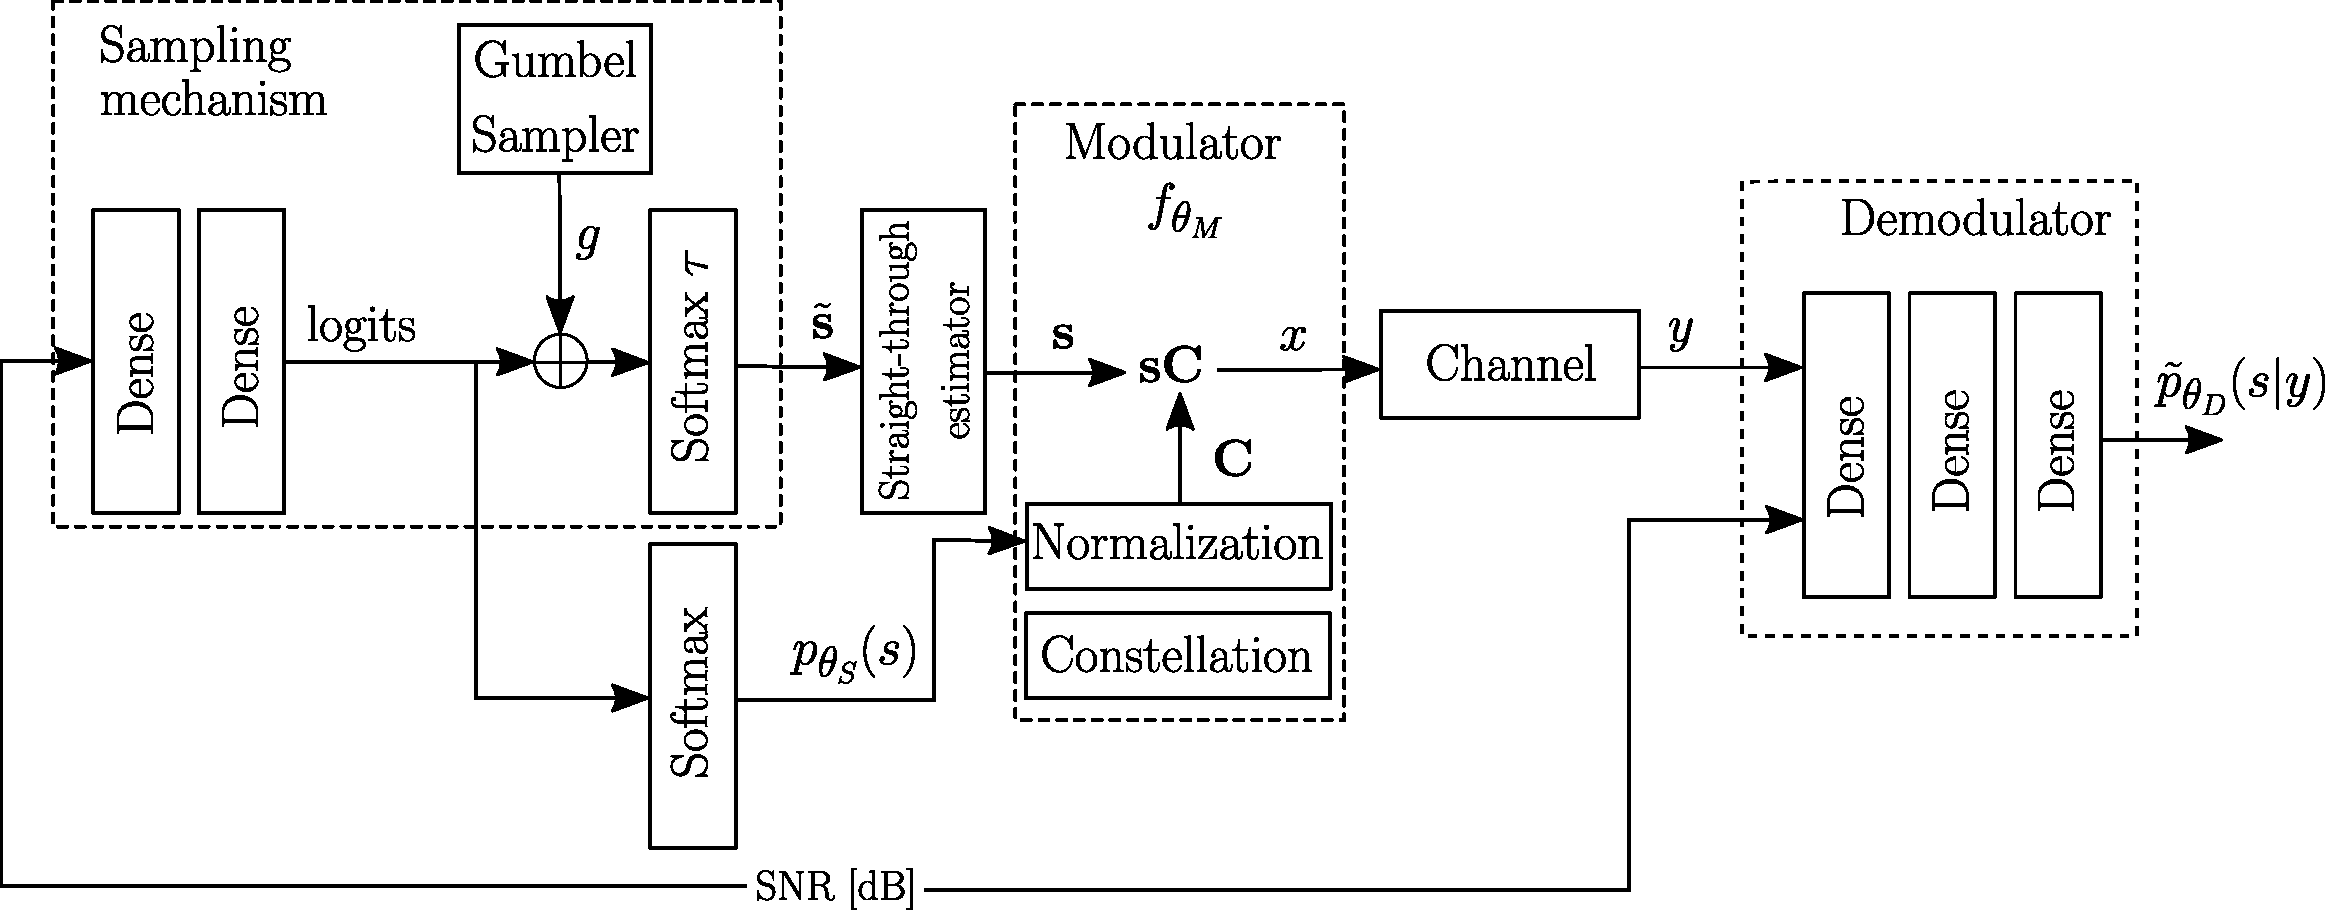
\includegraphics[width=\textwidth]{figs/stark_diagram.pdf}
	\centering	
	\caption{Proposed Autoencoder Architecture from \cite{Stark}}
	\label{fig:starkAe}
\end{figure}

\citeauthor{Stark}'s autoencoder is made up from three major blocks: sampler, modulator, and demodulator. Fig \ref{fig:starkAe} shows the complete architecture of the end-to-end system, where the trainable parameters $p_{\theta_S}(s), f_{\theta_M} \text{ and } p_{\theta_D}(s|y)$ correspond to our $P_M, C_M, \text{ and } D$, respectively. While the modulator and demodulator blocks are similar to the proposal from \cite{O'Shea}, the simultaneous probabilistic shaping is possible thanks to the careful design of the sampler. By ensuring that the sampler mechanism is differentiable, the gradients with respect to each $p_i \in P_M$ are precise when calculated via \cgls{sgd}. In fact, the differentiability is gained by leveraging the so-called \textit{Gumbel-Softmax trick} \cite{JANG}, which circunvents the need for using the arg-max function to sample the discrete distribution $P_M$.

We have implemented the end-to-end system using PyTorch \cite{PyTorch}. The sampler is made out of 2 layers. The first layer is made out of 128 units with ReLU activation, and the second layer of M units with linear activations. In the forward pass, the logit output is then processed through the Gumbel-Softmax trick and then through the straight-through estimator to produce the one-hot-encoded training set. While in the backward pass, the straight-through estimator uses the approximate one-hot vector ---the output of the Gumbel-Softmax block.  The trainable parameter of the sampler, $P_M$, is initialized to a uniform distribution.
The modulator is made out of a single linear layer of N units followed by a normalization operation to ensure that the energy constraint of the constellation is mantained, i.e.,
\begin{align}
	\sum\limits_{p_i \in P_M} p_i |x_i|^2.
\end{align}
If only probabilistic shaping is applied, the constellation remains fixed, e.g., M-\cgls{ask}, is used. On the contrary, when geometric shaping is performed, the parameter $C_M$ corresponds to the unnormalized constellation points.
Finally, the demodulator is made out of 3 layers. The first two layers are made out of 128 units with ReLU activations, and the third layer of M units with linear activation. The trainable parameter of the demodulator, $D$ corresponds to the \textit{a posteriori} probabilities $p(x|y)$.



\subsection{Autoencoder Performance}

Training was performed with the Adam optimizer and the hyper-parameters of the training are: learning-rate=0.001, batch-size=10000, and number of epochs=4000.
The resulting M-\cgls{ask} constellations for both only probabilistic and joint probabilistic and geometric shaping are presented in Figure \ref{fig:starkMASK}. Moreover the respective achieved \cgls{mi} for the corresponding M-\cgls{qam} scheme, i.e., 64-\cgls{qam}, are available in Figure \ref{fig:starkPerf} for SNR values ranging from 5dB to 22dB.
	
\begin{figure}[h]
	\subfigure[SNR = 5dB]{
         \scalebox{1}{%% Creator: Matplotlib, PGF backend
%%
%% To include the figure in your LaTeX document, write
%%   \input{<filename>.pgf}
%%
%% Make sure the required packages are loaded in your preamble
%%   \usepackage{pgf}
%%
%% Also ensure that all the required font packages are loaded; for instance,
%% the lmodern package is sometimes necessary when using math font.
%%   \usepackage{lmodern}
%%
%% Figures using additional raster images can only be included by \input if
%% they are in the same directory as the main LaTeX file. For loading figures
%% from other directories you can use the `import` package
%%   \usepackage{import}
%%
%% and then include the figures with
%%   \import{<path to file>}{<filename>.pgf}
%%
%% Matplotlib used the following preamble
%%
\begingroup%
\makeatletter%
\begin{pgfpicture}%
\pgfpathrectangle{\pgfpointorigin}{\pgfqpoint{3.000000in}{3.000000in}}%
\pgfusepath{use as bounding box, clip}%
\begin{pgfscope}%
\pgfsetbuttcap%
\pgfsetmiterjoin%
\pgfsetlinewidth{0.000000pt}%
\definecolor{currentstroke}{rgb}{1.000000,1.000000,1.000000}%
\pgfsetstrokecolor{currentstroke}%
\pgfsetstrokeopacity{0.000000}%
\pgfsetdash{}{0pt}%
\pgfpathmoveto{\pgfqpoint{0.000000in}{0.000000in}}%
\pgfpathlineto{\pgfqpoint{3.000000in}{0.000000in}}%
\pgfpathlineto{\pgfqpoint{3.000000in}{3.000000in}}%
\pgfpathlineto{\pgfqpoint{0.000000in}{3.000000in}}%
\pgfpathlineto{\pgfqpoint{0.000000in}{0.000000in}}%
\pgfpathclose%
\pgfusepath{}%
\end{pgfscope}%
\begin{pgfscope}%
\pgfsetbuttcap%
\pgfsetmiterjoin%
\definecolor{currentfill}{rgb}{1.000000,1.000000,1.000000}%
\pgfsetfillcolor{currentfill}%
\pgfsetlinewidth{0.000000pt}%
\definecolor{currentstroke}{rgb}{0.000000,0.000000,0.000000}%
\pgfsetstrokecolor{currentstroke}%
\pgfsetstrokeopacity{0.000000}%
\pgfsetdash{}{0pt}%
\pgfpathmoveto{\pgfqpoint{0.375000in}{0.375000in}}%
\pgfpathlineto{\pgfqpoint{2.700000in}{0.375000in}}%
\pgfpathlineto{\pgfqpoint{2.700000in}{2.640000in}}%
\pgfpathlineto{\pgfqpoint{0.375000in}{2.640000in}}%
\pgfpathlineto{\pgfqpoint{0.375000in}{0.375000in}}%
\pgfpathclose%
\pgfusepath{fill}%
\end{pgfscope}%
\begin{pgfscope}%
\pgfpathrectangle{\pgfqpoint{0.375000in}{0.375000in}}{\pgfqpoint{2.325000in}{2.265000in}}%
\pgfusepath{clip}%
\pgfsetbuttcap%
\pgfsetmiterjoin%
\definecolor{currentfill}{rgb}{0.121569,0.466667,0.705882}%
\pgfsetfillcolor{currentfill}%
\pgfsetlinewidth{0.000000pt}%
\definecolor{currentstroke}{rgb}{0.000000,0.000000,0.000000}%
\pgfsetstrokecolor{currentstroke}%
\pgfsetstrokeopacity{0.000000}%
\pgfsetdash{}{0pt}%
\pgfpathmoveto{\pgfqpoint{0.480682in}{0.375000in}}%
\pgfpathlineto{\pgfqpoint{0.501818in}{0.375000in}}%
\pgfpathlineto{\pgfqpoint{0.501818in}{0.563083in}}%
\pgfpathlineto{\pgfqpoint{0.480682in}{0.563083in}}%
\pgfpathlineto{\pgfqpoint{0.480682in}{0.375000in}}%
\pgfpathclose%
\pgfusepath{fill}%
\end{pgfscope}%
\begin{pgfscope}%
\pgfpathrectangle{\pgfqpoint{0.375000in}{0.375000in}}{\pgfqpoint{2.325000in}{2.265000in}}%
\pgfusepath{clip}%
\pgfsetbuttcap%
\pgfsetmiterjoin%
\definecolor{currentfill}{rgb}{0.121569,0.466667,0.705882}%
\pgfsetfillcolor{currentfill}%
\pgfsetlinewidth{0.000000pt}%
\definecolor{currentstroke}{rgb}{0.000000,0.000000,0.000000}%
\pgfsetstrokecolor{currentstroke}%
\pgfsetstrokeopacity{0.000000}%
\pgfsetdash{}{0pt}%
\pgfpathmoveto{\pgfqpoint{0.501818in}{0.375000in}}%
\pgfpathlineto{\pgfqpoint{0.522955in}{0.375000in}}%
\pgfpathlineto{\pgfqpoint{0.522955in}{0.375000in}}%
\pgfpathlineto{\pgfqpoint{0.501818in}{0.375000in}}%
\pgfpathlineto{\pgfqpoint{0.501818in}{0.375000in}}%
\pgfpathclose%
\pgfusepath{fill}%
\end{pgfscope}%
\begin{pgfscope}%
\pgfpathrectangle{\pgfqpoint{0.375000in}{0.375000in}}{\pgfqpoint{2.325000in}{2.265000in}}%
\pgfusepath{clip}%
\pgfsetbuttcap%
\pgfsetmiterjoin%
\definecolor{currentfill}{rgb}{0.121569,0.466667,0.705882}%
\pgfsetfillcolor{currentfill}%
\pgfsetlinewidth{0.000000pt}%
\definecolor{currentstroke}{rgb}{0.000000,0.000000,0.000000}%
\pgfsetstrokecolor{currentstroke}%
\pgfsetstrokeopacity{0.000000}%
\pgfsetdash{}{0pt}%
\pgfpathmoveto{\pgfqpoint{0.522955in}{0.375000in}}%
\pgfpathlineto{\pgfqpoint{0.544091in}{0.375000in}}%
\pgfpathlineto{\pgfqpoint{0.544091in}{0.375000in}}%
\pgfpathlineto{\pgfqpoint{0.522955in}{0.375000in}}%
\pgfpathlineto{\pgfqpoint{0.522955in}{0.375000in}}%
\pgfpathclose%
\pgfusepath{fill}%
\end{pgfscope}%
\begin{pgfscope}%
\pgfpathrectangle{\pgfqpoint{0.375000in}{0.375000in}}{\pgfqpoint{2.325000in}{2.265000in}}%
\pgfusepath{clip}%
\pgfsetbuttcap%
\pgfsetmiterjoin%
\definecolor{currentfill}{rgb}{0.121569,0.466667,0.705882}%
\pgfsetfillcolor{currentfill}%
\pgfsetlinewidth{0.000000pt}%
\definecolor{currentstroke}{rgb}{0.000000,0.000000,0.000000}%
\pgfsetstrokecolor{currentstroke}%
\pgfsetstrokeopacity{0.000000}%
\pgfsetdash{}{0pt}%
\pgfpathmoveto{\pgfqpoint{0.544091in}{0.375000in}}%
\pgfpathlineto{\pgfqpoint{0.565227in}{0.375000in}}%
\pgfpathlineto{\pgfqpoint{0.565227in}{0.375000in}}%
\pgfpathlineto{\pgfqpoint{0.544091in}{0.375000in}}%
\pgfpathlineto{\pgfqpoint{0.544091in}{0.375000in}}%
\pgfpathclose%
\pgfusepath{fill}%
\end{pgfscope}%
\begin{pgfscope}%
\pgfpathrectangle{\pgfqpoint{0.375000in}{0.375000in}}{\pgfqpoint{2.325000in}{2.265000in}}%
\pgfusepath{clip}%
\pgfsetbuttcap%
\pgfsetmiterjoin%
\definecolor{currentfill}{rgb}{0.121569,0.466667,0.705882}%
\pgfsetfillcolor{currentfill}%
\pgfsetlinewidth{0.000000pt}%
\definecolor{currentstroke}{rgb}{0.000000,0.000000,0.000000}%
\pgfsetstrokecolor{currentstroke}%
\pgfsetstrokeopacity{0.000000}%
\pgfsetdash{}{0pt}%
\pgfpathmoveto{\pgfqpoint{0.565227in}{0.375000in}}%
\pgfpathlineto{\pgfqpoint{0.586364in}{0.375000in}}%
\pgfpathlineto{\pgfqpoint{0.586364in}{0.375000in}}%
\pgfpathlineto{\pgfqpoint{0.565227in}{0.375000in}}%
\pgfpathlineto{\pgfqpoint{0.565227in}{0.375000in}}%
\pgfpathclose%
\pgfusepath{fill}%
\end{pgfscope}%
\begin{pgfscope}%
\pgfpathrectangle{\pgfqpoint{0.375000in}{0.375000in}}{\pgfqpoint{2.325000in}{2.265000in}}%
\pgfusepath{clip}%
\pgfsetbuttcap%
\pgfsetmiterjoin%
\definecolor{currentfill}{rgb}{0.121569,0.466667,0.705882}%
\pgfsetfillcolor{currentfill}%
\pgfsetlinewidth{0.000000pt}%
\definecolor{currentstroke}{rgb}{0.000000,0.000000,0.000000}%
\pgfsetstrokecolor{currentstroke}%
\pgfsetstrokeopacity{0.000000}%
\pgfsetdash{}{0pt}%
\pgfpathmoveto{\pgfqpoint{0.586364in}{0.375000in}}%
\pgfpathlineto{\pgfqpoint{0.607500in}{0.375000in}}%
\pgfpathlineto{\pgfqpoint{0.607500in}{0.375000in}}%
\pgfpathlineto{\pgfqpoint{0.586364in}{0.375000in}}%
\pgfpathlineto{\pgfqpoint{0.586364in}{0.375000in}}%
\pgfpathclose%
\pgfusepath{fill}%
\end{pgfscope}%
\begin{pgfscope}%
\pgfpathrectangle{\pgfqpoint{0.375000in}{0.375000in}}{\pgfqpoint{2.325000in}{2.265000in}}%
\pgfusepath{clip}%
\pgfsetbuttcap%
\pgfsetmiterjoin%
\definecolor{currentfill}{rgb}{0.121569,0.466667,0.705882}%
\pgfsetfillcolor{currentfill}%
\pgfsetlinewidth{0.000000pt}%
\definecolor{currentstroke}{rgb}{0.000000,0.000000,0.000000}%
\pgfsetstrokecolor{currentstroke}%
\pgfsetstrokeopacity{0.000000}%
\pgfsetdash{}{0pt}%
\pgfpathmoveto{\pgfqpoint{0.607500in}{0.375000in}}%
\pgfpathlineto{\pgfqpoint{0.628636in}{0.375000in}}%
\pgfpathlineto{\pgfqpoint{0.628636in}{0.375000in}}%
\pgfpathlineto{\pgfqpoint{0.607500in}{0.375000in}}%
\pgfpathlineto{\pgfqpoint{0.607500in}{0.375000in}}%
\pgfpathclose%
\pgfusepath{fill}%
\end{pgfscope}%
\begin{pgfscope}%
\pgfpathrectangle{\pgfqpoint{0.375000in}{0.375000in}}{\pgfqpoint{2.325000in}{2.265000in}}%
\pgfusepath{clip}%
\pgfsetbuttcap%
\pgfsetmiterjoin%
\definecolor{currentfill}{rgb}{0.121569,0.466667,0.705882}%
\pgfsetfillcolor{currentfill}%
\pgfsetlinewidth{0.000000pt}%
\definecolor{currentstroke}{rgb}{0.000000,0.000000,0.000000}%
\pgfsetstrokecolor{currentstroke}%
\pgfsetstrokeopacity{0.000000}%
\pgfsetdash{}{0pt}%
\pgfpathmoveto{\pgfqpoint{0.628636in}{0.375000in}}%
\pgfpathlineto{\pgfqpoint{0.649773in}{0.375000in}}%
\pgfpathlineto{\pgfqpoint{0.649773in}{0.375000in}}%
\pgfpathlineto{\pgfqpoint{0.628636in}{0.375000in}}%
\pgfpathlineto{\pgfqpoint{0.628636in}{0.375000in}}%
\pgfpathclose%
\pgfusepath{fill}%
\end{pgfscope}%
\begin{pgfscope}%
\pgfpathrectangle{\pgfqpoint{0.375000in}{0.375000in}}{\pgfqpoint{2.325000in}{2.265000in}}%
\pgfusepath{clip}%
\pgfsetbuttcap%
\pgfsetmiterjoin%
\definecolor{currentfill}{rgb}{0.121569,0.466667,0.705882}%
\pgfsetfillcolor{currentfill}%
\pgfsetlinewidth{0.000000pt}%
\definecolor{currentstroke}{rgb}{0.000000,0.000000,0.000000}%
\pgfsetstrokecolor{currentstroke}%
\pgfsetstrokeopacity{0.000000}%
\pgfsetdash{}{0pt}%
\pgfpathmoveto{\pgfqpoint{0.649773in}{0.375000in}}%
\pgfpathlineto{\pgfqpoint{0.670909in}{0.375000in}}%
\pgfpathlineto{\pgfqpoint{0.670909in}{0.375000in}}%
\pgfpathlineto{\pgfqpoint{0.649773in}{0.375000in}}%
\pgfpathlineto{\pgfqpoint{0.649773in}{0.375000in}}%
\pgfpathclose%
\pgfusepath{fill}%
\end{pgfscope}%
\begin{pgfscope}%
\pgfpathrectangle{\pgfqpoint{0.375000in}{0.375000in}}{\pgfqpoint{2.325000in}{2.265000in}}%
\pgfusepath{clip}%
\pgfsetbuttcap%
\pgfsetmiterjoin%
\definecolor{currentfill}{rgb}{0.121569,0.466667,0.705882}%
\pgfsetfillcolor{currentfill}%
\pgfsetlinewidth{0.000000pt}%
\definecolor{currentstroke}{rgb}{0.000000,0.000000,0.000000}%
\pgfsetstrokecolor{currentstroke}%
\pgfsetstrokeopacity{0.000000}%
\pgfsetdash{}{0pt}%
\pgfpathmoveto{\pgfqpoint{0.670909in}{0.375000in}}%
\pgfpathlineto{\pgfqpoint{0.692046in}{0.375000in}}%
\pgfpathlineto{\pgfqpoint{0.692046in}{0.375000in}}%
\pgfpathlineto{\pgfqpoint{0.670909in}{0.375000in}}%
\pgfpathlineto{\pgfqpoint{0.670909in}{0.375000in}}%
\pgfpathclose%
\pgfusepath{fill}%
\end{pgfscope}%
\begin{pgfscope}%
\pgfpathrectangle{\pgfqpoint{0.375000in}{0.375000in}}{\pgfqpoint{2.325000in}{2.265000in}}%
\pgfusepath{clip}%
\pgfsetbuttcap%
\pgfsetmiterjoin%
\definecolor{currentfill}{rgb}{0.121569,0.466667,0.705882}%
\pgfsetfillcolor{currentfill}%
\pgfsetlinewidth{0.000000pt}%
\definecolor{currentstroke}{rgb}{0.000000,0.000000,0.000000}%
\pgfsetstrokecolor{currentstroke}%
\pgfsetstrokeopacity{0.000000}%
\pgfsetdash{}{0pt}%
\pgfpathmoveto{\pgfqpoint{0.692046in}{0.375000in}}%
\pgfpathlineto{\pgfqpoint{0.713182in}{0.375000in}}%
\pgfpathlineto{\pgfqpoint{0.713182in}{0.375000in}}%
\pgfpathlineto{\pgfqpoint{0.692046in}{0.375000in}}%
\pgfpathlineto{\pgfqpoint{0.692046in}{0.375000in}}%
\pgfpathclose%
\pgfusepath{fill}%
\end{pgfscope}%
\begin{pgfscope}%
\pgfpathrectangle{\pgfqpoint{0.375000in}{0.375000in}}{\pgfqpoint{2.325000in}{2.265000in}}%
\pgfusepath{clip}%
\pgfsetbuttcap%
\pgfsetmiterjoin%
\definecolor{currentfill}{rgb}{0.121569,0.466667,0.705882}%
\pgfsetfillcolor{currentfill}%
\pgfsetlinewidth{0.000000pt}%
\definecolor{currentstroke}{rgb}{0.000000,0.000000,0.000000}%
\pgfsetstrokecolor{currentstroke}%
\pgfsetstrokeopacity{0.000000}%
\pgfsetdash{}{0pt}%
\pgfpathmoveto{\pgfqpoint{0.713182in}{0.375000in}}%
\pgfpathlineto{\pgfqpoint{0.734318in}{0.375000in}}%
\pgfpathlineto{\pgfqpoint{0.734318in}{0.375000in}}%
\pgfpathlineto{\pgfqpoint{0.713182in}{0.375000in}}%
\pgfpathlineto{\pgfqpoint{0.713182in}{0.375000in}}%
\pgfpathclose%
\pgfusepath{fill}%
\end{pgfscope}%
\begin{pgfscope}%
\pgfpathrectangle{\pgfqpoint{0.375000in}{0.375000in}}{\pgfqpoint{2.325000in}{2.265000in}}%
\pgfusepath{clip}%
\pgfsetbuttcap%
\pgfsetmiterjoin%
\definecolor{currentfill}{rgb}{0.121569,0.466667,0.705882}%
\pgfsetfillcolor{currentfill}%
\pgfsetlinewidth{0.000000pt}%
\definecolor{currentstroke}{rgb}{0.000000,0.000000,0.000000}%
\pgfsetstrokecolor{currentstroke}%
\pgfsetstrokeopacity{0.000000}%
\pgfsetdash{}{0pt}%
\pgfpathmoveto{\pgfqpoint{0.734318in}{0.375000in}}%
\pgfpathlineto{\pgfqpoint{0.755455in}{0.375000in}}%
\pgfpathlineto{\pgfqpoint{0.755455in}{0.375000in}}%
\pgfpathlineto{\pgfqpoint{0.734318in}{0.375000in}}%
\pgfpathlineto{\pgfqpoint{0.734318in}{0.375000in}}%
\pgfpathclose%
\pgfusepath{fill}%
\end{pgfscope}%
\begin{pgfscope}%
\pgfpathrectangle{\pgfqpoint{0.375000in}{0.375000in}}{\pgfqpoint{2.325000in}{2.265000in}}%
\pgfusepath{clip}%
\pgfsetbuttcap%
\pgfsetmiterjoin%
\definecolor{currentfill}{rgb}{0.121569,0.466667,0.705882}%
\pgfsetfillcolor{currentfill}%
\pgfsetlinewidth{0.000000pt}%
\definecolor{currentstroke}{rgb}{0.000000,0.000000,0.000000}%
\pgfsetstrokecolor{currentstroke}%
\pgfsetstrokeopacity{0.000000}%
\pgfsetdash{}{0pt}%
\pgfpathmoveto{\pgfqpoint{0.755455in}{0.375000in}}%
\pgfpathlineto{\pgfqpoint{0.776591in}{0.375000in}}%
\pgfpathlineto{\pgfqpoint{0.776591in}{0.375000in}}%
\pgfpathlineto{\pgfqpoint{0.755455in}{0.375000in}}%
\pgfpathlineto{\pgfqpoint{0.755455in}{0.375000in}}%
\pgfpathclose%
\pgfusepath{fill}%
\end{pgfscope}%
\begin{pgfscope}%
\pgfpathrectangle{\pgfqpoint{0.375000in}{0.375000in}}{\pgfqpoint{2.325000in}{2.265000in}}%
\pgfusepath{clip}%
\pgfsetbuttcap%
\pgfsetmiterjoin%
\definecolor{currentfill}{rgb}{0.121569,0.466667,0.705882}%
\pgfsetfillcolor{currentfill}%
\pgfsetlinewidth{0.000000pt}%
\definecolor{currentstroke}{rgb}{0.000000,0.000000,0.000000}%
\pgfsetstrokecolor{currentstroke}%
\pgfsetstrokeopacity{0.000000}%
\pgfsetdash{}{0pt}%
\pgfpathmoveto{\pgfqpoint{0.776591in}{0.375000in}}%
\pgfpathlineto{\pgfqpoint{0.797727in}{0.375000in}}%
\pgfpathlineto{\pgfqpoint{0.797727in}{0.375000in}}%
\pgfpathlineto{\pgfqpoint{0.776591in}{0.375000in}}%
\pgfpathlineto{\pgfqpoint{0.776591in}{0.375000in}}%
\pgfpathclose%
\pgfusepath{fill}%
\end{pgfscope}%
\begin{pgfscope}%
\pgfpathrectangle{\pgfqpoint{0.375000in}{0.375000in}}{\pgfqpoint{2.325000in}{2.265000in}}%
\pgfusepath{clip}%
\pgfsetbuttcap%
\pgfsetmiterjoin%
\definecolor{currentfill}{rgb}{0.121569,0.466667,0.705882}%
\pgfsetfillcolor{currentfill}%
\pgfsetlinewidth{0.000000pt}%
\definecolor{currentstroke}{rgb}{0.000000,0.000000,0.000000}%
\pgfsetstrokecolor{currentstroke}%
\pgfsetstrokeopacity{0.000000}%
\pgfsetdash{}{0pt}%
\pgfpathmoveto{\pgfqpoint{0.797727in}{0.375000in}}%
\pgfpathlineto{\pgfqpoint{0.818864in}{0.375000in}}%
\pgfpathlineto{\pgfqpoint{0.818864in}{0.375000in}}%
\pgfpathlineto{\pgfqpoint{0.797727in}{0.375000in}}%
\pgfpathlineto{\pgfqpoint{0.797727in}{0.375000in}}%
\pgfpathclose%
\pgfusepath{fill}%
\end{pgfscope}%
\begin{pgfscope}%
\pgfpathrectangle{\pgfqpoint{0.375000in}{0.375000in}}{\pgfqpoint{2.325000in}{2.265000in}}%
\pgfusepath{clip}%
\pgfsetbuttcap%
\pgfsetmiterjoin%
\definecolor{currentfill}{rgb}{0.121569,0.466667,0.705882}%
\pgfsetfillcolor{currentfill}%
\pgfsetlinewidth{0.000000pt}%
\definecolor{currentstroke}{rgb}{0.000000,0.000000,0.000000}%
\pgfsetstrokecolor{currentstroke}%
\pgfsetstrokeopacity{0.000000}%
\pgfsetdash{}{0pt}%
\pgfpathmoveto{\pgfqpoint{0.818864in}{0.375000in}}%
\pgfpathlineto{\pgfqpoint{0.840000in}{0.375000in}}%
\pgfpathlineto{\pgfqpoint{0.840000in}{0.375000in}}%
\pgfpathlineto{\pgfqpoint{0.818864in}{0.375000in}}%
\pgfpathlineto{\pgfqpoint{0.818864in}{0.375000in}}%
\pgfpathclose%
\pgfusepath{fill}%
\end{pgfscope}%
\begin{pgfscope}%
\pgfpathrectangle{\pgfqpoint{0.375000in}{0.375000in}}{\pgfqpoint{2.325000in}{2.265000in}}%
\pgfusepath{clip}%
\pgfsetbuttcap%
\pgfsetmiterjoin%
\definecolor{currentfill}{rgb}{0.121569,0.466667,0.705882}%
\pgfsetfillcolor{currentfill}%
\pgfsetlinewidth{0.000000pt}%
\definecolor{currentstroke}{rgb}{0.000000,0.000000,0.000000}%
\pgfsetstrokecolor{currentstroke}%
\pgfsetstrokeopacity{0.000000}%
\pgfsetdash{}{0pt}%
\pgfpathmoveto{\pgfqpoint{0.840000in}{0.375000in}}%
\pgfpathlineto{\pgfqpoint{0.861137in}{0.375000in}}%
\pgfpathlineto{\pgfqpoint{0.861137in}{0.375000in}}%
\pgfpathlineto{\pgfqpoint{0.840000in}{0.375000in}}%
\pgfpathlineto{\pgfqpoint{0.840000in}{0.375000in}}%
\pgfpathclose%
\pgfusepath{fill}%
\end{pgfscope}%
\begin{pgfscope}%
\pgfpathrectangle{\pgfqpoint{0.375000in}{0.375000in}}{\pgfqpoint{2.325000in}{2.265000in}}%
\pgfusepath{clip}%
\pgfsetbuttcap%
\pgfsetmiterjoin%
\definecolor{currentfill}{rgb}{0.121569,0.466667,0.705882}%
\pgfsetfillcolor{currentfill}%
\pgfsetlinewidth{0.000000pt}%
\definecolor{currentstroke}{rgb}{0.000000,0.000000,0.000000}%
\pgfsetstrokecolor{currentstroke}%
\pgfsetstrokeopacity{0.000000}%
\pgfsetdash{}{0pt}%
\pgfpathmoveto{\pgfqpoint{0.861136in}{0.375000in}}%
\pgfpathlineto{\pgfqpoint{0.882273in}{0.375000in}}%
\pgfpathlineto{\pgfqpoint{0.882273in}{0.375000in}}%
\pgfpathlineto{\pgfqpoint{0.861136in}{0.375000in}}%
\pgfpathlineto{\pgfqpoint{0.861136in}{0.375000in}}%
\pgfpathclose%
\pgfusepath{fill}%
\end{pgfscope}%
\begin{pgfscope}%
\pgfpathrectangle{\pgfqpoint{0.375000in}{0.375000in}}{\pgfqpoint{2.325000in}{2.265000in}}%
\pgfusepath{clip}%
\pgfsetbuttcap%
\pgfsetmiterjoin%
\definecolor{currentfill}{rgb}{0.121569,0.466667,0.705882}%
\pgfsetfillcolor{currentfill}%
\pgfsetlinewidth{0.000000pt}%
\definecolor{currentstroke}{rgb}{0.000000,0.000000,0.000000}%
\pgfsetstrokecolor{currentstroke}%
\pgfsetstrokeopacity{0.000000}%
\pgfsetdash{}{0pt}%
\pgfpathmoveto{\pgfqpoint{0.882273in}{0.375000in}}%
\pgfpathlineto{\pgfqpoint{0.903409in}{0.375000in}}%
\pgfpathlineto{\pgfqpoint{0.903409in}{1.231071in}}%
\pgfpathlineto{\pgfqpoint{0.882273in}{1.231071in}}%
\pgfpathlineto{\pgfqpoint{0.882273in}{0.375000in}}%
\pgfpathclose%
\pgfusepath{fill}%
\end{pgfscope}%
\begin{pgfscope}%
\pgfpathrectangle{\pgfqpoint{0.375000in}{0.375000in}}{\pgfqpoint{2.325000in}{2.265000in}}%
\pgfusepath{clip}%
\pgfsetbuttcap%
\pgfsetmiterjoin%
\definecolor{currentfill}{rgb}{0.121569,0.466667,0.705882}%
\pgfsetfillcolor{currentfill}%
\pgfsetlinewidth{0.000000pt}%
\definecolor{currentstroke}{rgb}{0.000000,0.000000,0.000000}%
\pgfsetstrokecolor{currentstroke}%
\pgfsetstrokeopacity{0.000000}%
\pgfsetdash{}{0pt}%
\pgfpathmoveto{\pgfqpoint{0.903409in}{0.375000in}}%
\pgfpathlineto{\pgfqpoint{0.924546in}{0.375000in}}%
\pgfpathlineto{\pgfqpoint{0.924546in}{0.375000in}}%
\pgfpathlineto{\pgfqpoint{0.903409in}{0.375000in}}%
\pgfpathlineto{\pgfqpoint{0.903409in}{0.375000in}}%
\pgfpathclose%
\pgfusepath{fill}%
\end{pgfscope}%
\begin{pgfscope}%
\pgfpathrectangle{\pgfqpoint{0.375000in}{0.375000in}}{\pgfqpoint{2.325000in}{2.265000in}}%
\pgfusepath{clip}%
\pgfsetbuttcap%
\pgfsetmiterjoin%
\definecolor{currentfill}{rgb}{0.121569,0.466667,0.705882}%
\pgfsetfillcolor{currentfill}%
\pgfsetlinewidth{0.000000pt}%
\definecolor{currentstroke}{rgb}{0.000000,0.000000,0.000000}%
\pgfsetstrokecolor{currentstroke}%
\pgfsetstrokeopacity{0.000000}%
\pgfsetdash{}{0pt}%
\pgfpathmoveto{\pgfqpoint{0.924546in}{0.375000in}}%
\pgfpathlineto{\pgfqpoint{0.945682in}{0.375000in}}%
\pgfpathlineto{\pgfqpoint{0.945682in}{0.375000in}}%
\pgfpathlineto{\pgfqpoint{0.924546in}{0.375000in}}%
\pgfpathlineto{\pgfqpoint{0.924546in}{0.375000in}}%
\pgfpathclose%
\pgfusepath{fill}%
\end{pgfscope}%
\begin{pgfscope}%
\pgfpathrectangle{\pgfqpoint{0.375000in}{0.375000in}}{\pgfqpoint{2.325000in}{2.265000in}}%
\pgfusepath{clip}%
\pgfsetbuttcap%
\pgfsetmiterjoin%
\definecolor{currentfill}{rgb}{0.121569,0.466667,0.705882}%
\pgfsetfillcolor{currentfill}%
\pgfsetlinewidth{0.000000pt}%
\definecolor{currentstroke}{rgb}{0.000000,0.000000,0.000000}%
\pgfsetstrokecolor{currentstroke}%
\pgfsetstrokeopacity{0.000000}%
\pgfsetdash{}{0pt}%
\pgfpathmoveto{\pgfqpoint{0.945682in}{0.375000in}}%
\pgfpathlineto{\pgfqpoint{0.966818in}{0.375000in}}%
\pgfpathlineto{\pgfqpoint{0.966818in}{0.375000in}}%
\pgfpathlineto{\pgfqpoint{0.945682in}{0.375000in}}%
\pgfpathlineto{\pgfqpoint{0.945682in}{0.375000in}}%
\pgfpathclose%
\pgfusepath{fill}%
\end{pgfscope}%
\begin{pgfscope}%
\pgfpathrectangle{\pgfqpoint{0.375000in}{0.375000in}}{\pgfqpoint{2.325000in}{2.265000in}}%
\pgfusepath{clip}%
\pgfsetbuttcap%
\pgfsetmiterjoin%
\definecolor{currentfill}{rgb}{0.121569,0.466667,0.705882}%
\pgfsetfillcolor{currentfill}%
\pgfsetlinewidth{0.000000pt}%
\definecolor{currentstroke}{rgb}{0.000000,0.000000,0.000000}%
\pgfsetstrokecolor{currentstroke}%
\pgfsetstrokeopacity{0.000000}%
\pgfsetdash{}{0pt}%
\pgfpathmoveto{\pgfqpoint{0.966818in}{0.375000in}}%
\pgfpathlineto{\pgfqpoint{0.987955in}{0.375000in}}%
\pgfpathlineto{\pgfqpoint{0.987955in}{0.375000in}}%
\pgfpathlineto{\pgfqpoint{0.966818in}{0.375000in}}%
\pgfpathlineto{\pgfqpoint{0.966818in}{0.375000in}}%
\pgfpathclose%
\pgfusepath{fill}%
\end{pgfscope}%
\begin{pgfscope}%
\pgfpathrectangle{\pgfqpoint{0.375000in}{0.375000in}}{\pgfqpoint{2.325000in}{2.265000in}}%
\pgfusepath{clip}%
\pgfsetbuttcap%
\pgfsetmiterjoin%
\definecolor{currentfill}{rgb}{0.121569,0.466667,0.705882}%
\pgfsetfillcolor{currentfill}%
\pgfsetlinewidth{0.000000pt}%
\definecolor{currentstroke}{rgb}{0.000000,0.000000,0.000000}%
\pgfsetstrokecolor{currentstroke}%
\pgfsetstrokeopacity{0.000000}%
\pgfsetdash{}{0pt}%
\pgfpathmoveto{\pgfqpoint{0.987955in}{0.375000in}}%
\pgfpathlineto{\pgfqpoint{1.009091in}{0.375000in}}%
\pgfpathlineto{\pgfqpoint{1.009091in}{0.375000in}}%
\pgfpathlineto{\pgfqpoint{0.987955in}{0.375000in}}%
\pgfpathlineto{\pgfqpoint{0.987955in}{0.375000in}}%
\pgfpathclose%
\pgfusepath{fill}%
\end{pgfscope}%
\begin{pgfscope}%
\pgfpathrectangle{\pgfqpoint{0.375000in}{0.375000in}}{\pgfqpoint{2.325000in}{2.265000in}}%
\pgfusepath{clip}%
\pgfsetbuttcap%
\pgfsetmiterjoin%
\definecolor{currentfill}{rgb}{0.121569,0.466667,0.705882}%
\pgfsetfillcolor{currentfill}%
\pgfsetlinewidth{0.000000pt}%
\definecolor{currentstroke}{rgb}{0.000000,0.000000,0.000000}%
\pgfsetstrokecolor{currentstroke}%
\pgfsetstrokeopacity{0.000000}%
\pgfsetdash{}{0pt}%
\pgfpathmoveto{\pgfqpoint{1.009091in}{0.375000in}}%
\pgfpathlineto{\pgfqpoint{1.030227in}{0.375000in}}%
\pgfpathlineto{\pgfqpoint{1.030227in}{0.375000in}}%
\pgfpathlineto{\pgfqpoint{1.009091in}{0.375000in}}%
\pgfpathlineto{\pgfqpoint{1.009091in}{0.375000in}}%
\pgfpathclose%
\pgfusepath{fill}%
\end{pgfscope}%
\begin{pgfscope}%
\pgfpathrectangle{\pgfqpoint{0.375000in}{0.375000in}}{\pgfqpoint{2.325000in}{2.265000in}}%
\pgfusepath{clip}%
\pgfsetbuttcap%
\pgfsetmiterjoin%
\definecolor{currentfill}{rgb}{0.121569,0.466667,0.705882}%
\pgfsetfillcolor{currentfill}%
\pgfsetlinewidth{0.000000pt}%
\definecolor{currentstroke}{rgb}{0.000000,0.000000,0.000000}%
\pgfsetstrokecolor{currentstroke}%
\pgfsetstrokeopacity{0.000000}%
\pgfsetdash{}{0pt}%
\pgfpathmoveto{\pgfqpoint{1.030227in}{0.375000in}}%
\pgfpathlineto{\pgfqpoint{1.051364in}{0.375000in}}%
\pgfpathlineto{\pgfqpoint{1.051364in}{0.375000in}}%
\pgfpathlineto{\pgfqpoint{1.030227in}{0.375000in}}%
\pgfpathlineto{\pgfqpoint{1.030227in}{0.375000in}}%
\pgfpathclose%
\pgfusepath{fill}%
\end{pgfscope}%
\begin{pgfscope}%
\pgfpathrectangle{\pgfqpoint{0.375000in}{0.375000in}}{\pgfqpoint{2.325000in}{2.265000in}}%
\pgfusepath{clip}%
\pgfsetbuttcap%
\pgfsetmiterjoin%
\definecolor{currentfill}{rgb}{0.121569,0.466667,0.705882}%
\pgfsetfillcolor{currentfill}%
\pgfsetlinewidth{0.000000pt}%
\definecolor{currentstroke}{rgb}{0.000000,0.000000,0.000000}%
\pgfsetstrokecolor{currentstroke}%
\pgfsetstrokeopacity{0.000000}%
\pgfsetdash{}{0pt}%
\pgfpathmoveto{\pgfqpoint{1.051364in}{0.375000in}}%
\pgfpathlineto{\pgfqpoint{1.072500in}{0.375000in}}%
\pgfpathlineto{\pgfqpoint{1.072500in}{0.375000in}}%
\pgfpathlineto{\pgfqpoint{1.051364in}{0.375000in}}%
\pgfpathlineto{\pgfqpoint{1.051364in}{0.375000in}}%
\pgfpathclose%
\pgfusepath{fill}%
\end{pgfscope}%
\begin{pgfscope}%
\pgfpathrectangle{\pgfqpoint{0.375000in}{0.375000in}}{\pgfqpoint{2.325000in}{2.265000in}}%
\pgfusepath{clip}%
\pgfsetbuttcap%
\pgfsetmiterjoin%
\definecolor{currentfill}{rgb}{0.121569,0.466667,0.705882}%
\pgfsetfillcolor{currentfill}%
\pgfsetlinewidth{0.000000pt}%
\definecolor{currentstroke}{rgb}{0.000000,0.000000,0.000000}%
\pgfsetstrokecolor{currentstroke}%
\pgfsetstrokeopacity{0.000000}%
\pgfsetdash{}{0pt}%
\pgfpathmoveto{\pgfqpoint{1.072500in}{0.375000in}}%
\pgfpathlineto{\pgfqpoint{1.093636in}{0.375000in}}%
\pgfpathlineto{\pgfqpoint{1.093636in}{0.375000in}}%
\pgfpathlineto{\pgfqpoint{1.072500in}{0.375000in}}%
\pgfpathlineto{\pgfqpoint{1.072500in}{0.375000in}}%
\pgfpathclose%
\pgfusepath{fill}%
\end{pgfscope}%
\begin{pgfscope}%
\pgfpathrectangle{\pgfqpoint{0.375000in}{0.375000in}}{\pgfqpoint{2.325000in}{2.265000in}}%
\pgfusepath{clip}%
\pgfsetbuttcap%
\pgfsetmiterjoin%
\definecolor{currentfill}{rgb}{0.121569,0.466667,0.705882}%
\pgfsetfillcolor{currentfill}%
\pgfsetlinewidth{0.000000pt}%
\definecolor{currentstroke}{rgb}{0.000000,0.000000,0.000000}%
\pgfsetstrokecolor{currentstroke}%
\pgfsetstrokeopacity{0.000000}%
\pgfsetdash{}{0pt}%
\pgfpathmoveto{\pgfqpoint{1.093636in}{0.375000in}}%
\pgfpathlineto{\pgfqpoint{1.114773in}{0.375000in}}%
\pgfpathlineto{\pgfqpoint{1.114773in}{0.375000in}}%
\pgfpathlineto{\pgfqpoint{1.093636in}{0.375000in}}%
\pgfpathlineto{\pgfqpoint{1.093636in}{0.375000in}}%
\pgfpathclose%
\pgfusepath{fill}%
\end{pgfscope}%
\begin{pgfscope}%
\pgfpathrectangle{\pgfqpoint{0.375000in}{0.375000in}}{\pgfqpoint{2.325000in}{2.265000in}}%
\pgfusepath{clip}%
\pgfsetbuttcap%
\pgfsetmiterjoin%
\definecolor{currentfill}{rgb}{0.121569,0.466667,0.705882}%
\pgfsetfillcolor{currentfill}%
\pgfsetlinewidth{0.000000pt}%
\definecolor{currentstroke}{rgb}{0.000000,0.000000,0.000000}%
\pgfsetstrokecolor{currentstroke}%
\pgfsetstrokeopacity{0.000000}%
\pgfsetdash{}{0pt}%
\pgfpathmoveto{\pgfqpoint{1.114773in}{0.375000in}}%
\pgfpathlineto{\pgfqpoint{1.135909in}{0.375000in}}%
\pgfpathlineto{\pgfqpoint{1.135909in}{0.375000in}}%
\pgfpathlineto{\pgfqpoint{1.114773in}{0.375000in}}%
\pgfpathlineto{\pgfqpoint{1.114773in}{0.375000in}}%
\pgfpathclose%
\pgfusepath{fill}%
\end{pgfscope}%
\begin{pgfscope}%
\pgfpathrectangle{\pgfqpoint{0.375000in}{0.375000in}}{\pgfqpoint{2.325000in}{2.265000in}}%
\pgfusepath{clip}%
\pgfsetbuttcap%
\pgfsetmiterjoin%
\definecolor{currentfill}{rgb}{0.121569,0.466667,0.705882}%
\pgfsetfillcolor{currentfill}%
\pgfsetlinewidth{0.000000pt}%
\definecolor{currentstroke}{rgb}{0.000000,0.000000,0.000000}%
\pgfsetstrokecolor{currentstroke}%
\pgfsetstrokeopacity{0.000000}%
\pgfsetdash{}{0pt}%
\pgfpathmoveto{\pgfqpoint{1.135909in}{0.375000in}}%
\pgfpathlineto{\pgfqpoint{1.157046in}{0.375000in}}%
\pgfpathlineto{\pgfqpoint{1.157046in}{0.375000in}}%
\pgfpathlineto{\pgfqpoint{1.135909in}{0.375000in}}%
\pgfpathlineto{\pgfqpoint{1.135909in}{0.375000in}}%
\pgfpathclose%
\pgfusepath{fill}%
\end{pgfscope}%
\begin{pgfscope}%
\pgfpathrectangle{\pgfqpoint{0.375000in}{0.375000in}}{\pgfqpoint{2.325000in}{2.265000in}}%
\pgfusepath{clip}%
\pgfsetbuttcap%
\pgfsetmiterjoin%
\definecolor{currentfill}{rgb}{0.121569,0.466667,0.705882}%
\pgfsetfillcolor{currentfill}%
\pgfsetlinewidth{0.000000pt}%
\definecolor{currentstroke}{rgb}{0.000000,0.000000,0.000000}%
\pgfsetstrokecolor{currentstroke}%
\pgfsetstrokeopacity{0.000000}%
\pgfsetdash{}{0pt}%
\pgfpathmoveto{\pgfqpoint{1.157046in}{0.375000in}}%
\pgfpathlineto{\pgfqpoint{1.178182in}{0.375000in}}%
\pgfpathlineto{\pgfqpoint{1.178182in}{2.082294in}}%
\pgfpathlineto{\pgfqpoint{1.157046in}{2.082294in}}%
\pgfpathlineto{\pgfqpoint{1.157046in}{0.375000in}}%
\pgfpathclose%
\pgfusepath{fill}%
\end{pgfscope}%
\begin{pgfscope}%
\pgfpathrectangle{\pgfqpoint{0.375000in}{0.375000in}}{\pgfqpoint{2.325000in}{2.265000in}}%
\pgfusepath{clip}%
\pgfsetbuttcap%
\pgfsetmiterjoin%
\definecolor{currentfill}{rgb}{0.121569,0.466667,0.705882}%
\pgfsetfillcolor{currentfill}%
\pgfsetlinewidth{0.000000pt}%
\definecolor{currentstroke}{rgb}{0.000000,0.000000,0.000000}%
\pgfsetstrokecolor{currentstroke}%
\pgfsetstrokeopacity{0.000000}%
\pgfsetdash{}{0pt}%
\pgfpathmoveto{\pgfqpoint{1.178182in}{0.375000in}}%
\pgfpathlineto{\pgfqpoint{1.199318in}{0.375000in}}%
\pgfpathlineto{\pgfqpoint{1.199318in}{0.375000in}}%
\pgfpathlineto{\pgfqpoint{1.178182in}{0.375000in}}%
\pgfpathlineto{\pgfqpoint{1.178182in}{0.375000in}}%
\pgfpathclose%
\pgfusepath{fill}%
\end{pgfscope}%
\begin{pgfscope}%
\pgfpathrectangle{\pgfqpoint{0.375000in}{0.375000in}}{\pgfqpoint{2.325000in}{2.265000in}}%
\pgfusepath{clip}%
\pgfsetbuttcap%
\pgfsetmiterjoin%
\definecolor{currentfill}{rgb}{0.121569,0.466667,0.705882}%
\pgfsetfillcolor{currentfill}%
\pgfsetlinewidth{0.000000pt}%
\definecolor{currentstroke}{rgb}{0.000000,0.000000,0.000000}%
\pgfsetstrokecolor{currentstroke}%
\pgfsetstrokeopacity{0.000000}%
\pgfsetdash{}{0pt}%
\pgfpathmoveto{\pgfqpoint{1.199318in}{0.375000in}}%
\pgfpathlineto{\pgfqpoint{1.220455in}{0.375000in}}%
\pgfpathlineto{\pgfqpoint{1.220455in}{0.375000in}}%
\pgfpathlineto{\pgfqpoint{1.199318in}{0.375000in}}%
\pgfpathlineto{\pgfqpoint{1.199318in}{0.375000in}}%
\pgfpathclose%
\pgfusepath{fill}%
\end{pgfscope}%
\begin{pgfscope}%
\pgfpathrectangle{\pgfqpoint{0.375000in}{0.375000in}}{\pgfqpoint{2.325000in}{2.265000in}}%
\pgfusepath{clip}%
\pgfsetbuttcap%
\pgfsetmiterjoin%
\definecolor{currentfill}{rgb}{0.121569,0.466667,0.705882}%
\pgfsetfillcolor{currentfill}%
\pgfsetlinewidth{0.000000pt}%
\definecolor{currentstroke}{rgb}{0.000000,0.000000,0.000000}%
\pgfsetstrokecolor{currentstroke}%
\pgfsetstrokeopacity{0.000000}%
\pgfsetdash{}{0pt}%
\pgfpathmoveto{\pgfqpoint{1.220455in}{0.375000in}}%
\pgfpathlineto{\pgfqpoint{1.241591in}{0.375000in}}%
\pgfpathlineto{\pgfqpoint{1.241591in}{0.375000in}}%
\pgfpathlineto{\pgfqpoint{1.220455in}{0.375000in}}%
\pgfpathlineto{\pgfqpoint{1.220455in}{0.375000in}}%
\pgfpathclose%
\pgfusepath{fill}%
\end{pgfscope}%
\begin{pgfscope}%
\pgfpathrectangle{\pgfqpoint{0.375000in}{0.375000in}}{\pgfqpoint{2.325000in}{2.265000in}}%
\pgfusepath{clip}%
\pgfsetbuttcap%
\pgfsetmiterjoin%
\definecolor{currentfill}{rgb}{0.121569,0.466667,0.705882}%
\pgfsetfillcolor{currentfill}%
\pgfsetlinewidth{0.000000pt}%
\definecolor{currentstroke}{rgb}{0.000000,0.000000,0.000000}%
\pgfsetstrokecolor{currentstroke}%
\pgfsetstrokeopacity{0.000000}%
\pgfsetdash{}{0pt}%
\pgfpathmoveto{\pgfqpoint{1.241591in}{0.375000in}}%
\pgfpathlineto{\pgfqpoint{1.262727in}{0.375000in}}%
\pgfpathlineto{\pgfqpoint{1.262727in}{0.375000in}}%
\pgfpathlineto{\pgfqpoint{1.241591in}{0.375000in}}%
\pgfpathlineto{\pgfqpoint{1.241591in}{0.375000in}}%
\pgfpathclose%
\pgfusepath{fill}%
\end{pgfscope}%
\begin{pgfscope}%
\pgfpathrectangle{\pgfqpoint{0.375000in}{0.375000in}}{\pgfqpoint{2.325000in}{2.265000in}}%
\pgfusepath{clip}%
\pgfsetbuttcap%
\pgfsetmiterjoin%
\definecolor{currentfill}{rgb}{0.121569,0.466667,0.705882}%
\pgfsetfillcolor{currentfill}%
\pgfsetlinewidth{0.000000pt}%
\definecolor{currentstroke}{rgb}{0.000000,0.000000,0.000000}%
\pgfsetstrokecolor{currentstroke}%
\pgfsetstrokeopacity{0.000000}%
\pgfsetdash{}{0pt}%
\pgfpathmoveto{\pgfqpoint{1.262727in}{0.375000in}}%
\pgfpathlineto{\pgfqpoint{1.283864in}{0.375000in}}%
\pgfpathlineto{\pgfqpoint{1.283864in}{0.375000in}}%
\pgfpathlineto{\pgfqpoint{1.262727in}{0.375000in}}%
\pgfpathlineto{\pgfqpoint{1.262727in}{0.375000in}}%
\pgfpathclose%
\pgfusepath{fill}%
\end{pgfscope}%
\begin{pgfscope}%
\pgfpathrectangle{\pgfqpoint{0.375000in}{0.375000in}}{\pgfqpoint{2.325000in}{2.265000in}}%
\pgfusepath{clip}%
\pgfsetbuttcap%
\pgfsetmiterjoin%
\definecolor{currentfill}{rgb}{0.121569,0.466667,0.705882}%
\pgfsetfillcolor{currentfill}%
\pgfsetlinewidth{0.000000pt}%
\definecolor{currentstroke}{rgb}{0.000000,0.000000,0.000000}%
\pgfsetstrokecolor{currentstroke}%
\pgfsetstrokeopacity{0.000000}%
\pgfsetdash{}{0pt}%
\pgfpathmoveto{\pgfqpoint{1.283864in}{0.375000in}}%
\pgfpathlineto{\pgfqpoint{1.305000in}{0.375000in}}%
\pgfpathlineto{\pgfqpoint{1.305000in}{0.375000in}}%
\pgfpathlineto{\pgfqpoint{1.283864in}{0.375000in}}%
\pgfpathlineto{\pgfqpoint{1.283864in}{0.375000in}}%
\pgfpathclose%
\pgfusepath{fill}%
\end{pgfscope}%
\begin{pgfscope}%
\pgfpathrectangle{\pgfqpoint{0.375000in}{0.375000in}}{\pgfqpoint{2.325000in}{2.265000in}}%
\pgfusepath{clip}%
\pgfsetbuttcap%
\pgfsetmiterjoin%
\definecolor{currentfill}{rgb}{0.121569,0.466667,0.705882}%
\pgfsetfillcolor{currentfill}%
\pgfsetlinewidth{0.000000pt}%
\definecolor{currentstroke}{rgb}{0.000000,0.000000,0.000000}%
\pgfsetstrokecolor{currentstroke}%
\pgfsetstrokeopacity{0.000000}%
\pgfsetdash{}{0pt}%
\pgfpathmoveto{\pgfqpoint{1.305000in}{0.375000in}}%
\pgfpathlineto{\pgfqpoint{1.326136in}{0.375000in}}%
\pgfpathlineto{\pgfqpoint{1.326136in}{0.375000in}}%
\pgfpathlineto{\pgfqpoint{1.305000in}{0.375000in}}%
\pgfpathlineto{\pgfqpoint{1.305000in}{0.375000in}}%
\pgfpathclose%
\pgfusepath{fill}%
\end{pgfscope}%
\begin{pgfscope}%
\pgfpathrectangle{\pgfqpoint{0.375000in}{0.375000in}}{\pgfqpoint{2.325000in}{2.265000in}}%
\pgfusepath{clip}%
\pgfsetbuttcap%
\pgfsetmiterjoin%
\definecolor{currentfill}{rgb}{0.121569,0.466667,0.705882}%
\pgfsetfillcolor{currentfill}%
\pgfsetlinewidth{0.000000pt}%
\definecolor{currentstroke}{rgb}{0.000000,0.000000,0.000000}%
\pgfsetstrokecolor{currentstroke}%
\pgfsetstrokeopacity{0.000000}%
\pgfsetdash{}{0pt}%
\pgfpathmoveto{\pgfqpoint{1.326136in}{0.375000in}}%
\pgfpathlineto{\pgfqpoint{1.347273in}{0.375000in}}%
\pgfpathlineto{\pgfqpoint{1.347273in}{0.375000in}}%
\pgfpathlineto{\pgfqpoint{1.326136in}{0.375000in}}%
\pgfpathlineto{\pgfqpoint{1.326136in}{0.375000in}}%
\pgfpathclose%
\pgfusepath{fill}%
\end{pgfscope}%
\begin{pgfscope}%
\pgfpathrectangle{\pgfqpoint{0.375000in}{0.375000in}}{\pgfqpoint{2.325000in}{2.265000in}}%
\pgfusepath{clip}%
\pgfsetbuttcap%
\pgfsetmiterjoin%
\definecolor{currentfill}{rgb}{0.121569,0.466667,0.705882}%
\pgfsetfillcolor{currentfill}%
\pgfsetlinewidth{0.000000pt}%
\definecolor{currentstroke}{rgb}{0.000000,0.000000,0.000000}%
\pgfsetstrokecolor{currentstroke}%
\pgfsetstrokeopacity{0.000000}%
\pgfsetdash{}{0pt}%
\pgfpathmoveto{\pgfqpoint{1.347273in}{0.375000in}}%
\pgfpathlineto{\pgfqpoint{1.368409in}{0.375000in}}%
\pgfpathlineto{\pgfqpoint{1.368409in}{0.375000in}}%
\pgfpathlineto{\pgfqpoint{1.347273in}{0.375000in}}%
\pgfpathlineto{\pgfqpoint{1.347273in}{0.375000in}}%
\pgfpathclose%
\pgfusepath{fill}%
\end{pgfscope}%
\begin{pgfscope}%
\pgfpathrectangle{\pgfqpoint{0.375000in}{0.375000in}}{\pgfqpoint{2.325000in}{2.265000in}}%
\pgfusepath{clip}%
\pgfsetbuttcap%
\pgfsetmiterjoin%
\definecolor{currentfill}{rgb}{0.121569,0.466667,0.705882}%
\pgfsetfillcolor{currentfill}%
\pgfsetlinewidth{0.000000pt}%
\definecolor{currentstroke}{rgb}{0.000000,0.000000,0.000000}%
\pgfsetstrokecolor{currentstroke}%
\pgfsetstrokeopacity{0.000000}%
\pgfsetdash{}{0pt}%
\pgfpathmoveto{\pgfqpoint{1.368409in}{0.375000in}}%
\pgfpathlineto{\pgfqpoint{1.389546in}{0.375000in}}%
\pgfpathlineto{\pgfqpoint{1.389546in}{0.375000in}}%
\pgfpathlineto{\pgfqpoint{1.368409in}{0.375000in}}%
\pgfpathlineto{\pgfqpoint{1.368409in}{0.375000in}}%
\pgfpathclose%
\pgfusepath{fill}%
\end{pgfscope}%
\begin{pgfscope}%
\pgfpathrectangle{\pgfqpoint{0.375000in}{0.375000in}}{\pgfqpoint{2.325000in}{2.265000in}}%
\pgfusepath{clip}%
\pgfsetbuttcap%
\pgfsetmiterjoin%
\definecolor{currentfill}{rgb}{0.121569,0.466667,0.705882}%
\pgfsetfillcolor{currentfill}%
\pgfsetlinewidth{0.000000pt}%
\definecolor{currentstroke}{rgb}{0.000000,0.000000,0.000000}%
\pgfsetstrokecolor{currentstroke}%
\pgfsetstrokeopacity{0.000000}%
\pgfsetdash{}{0pt}%
\pgfpathmoveto{\pgfqpoint{1.389546in}{0.375000in}}%
\pgfpathlineto{\pgfqpoint{1.410682in}{0.375000in}}%
\pgfpathlineto{\pgfqpoint{1.410682in}{0.375000in}}%
\pgfpathlineto{\pgfqpoint{1.389546in}{0.375000in}}%
\pgfpathlineto{\pgfqpoint{1.389546in}{0.375000in}}%
\pgfpathclose%
\pgfusepath{fill}%
\end{pgfscope}%
\begin{pgfscope}%
\pgfpathrectangle{\pgfqpoint{0.375000in}{0.375000in}}{\pgfqpoint{2.325000in}{2.265000in}}%
\pgfusepath{clip}%
\pgfsetbuttcap%
\pgfsetmiterjoin%
\definecolor{currentfill}{rgb}{0.121569,0.466667,0.705882}%
\pgfsetfillcolor{currentfill}%
\pgfsetlinewidth{0.000000pt}%
\definecolor{currentstroke}{rgb}{0.000000,0.000000,0.000000}%
\pgfsetstrokecolor{currentstroke}%
\pgfsetstrokeopacity{0.000000}%
\pgfsetdash{}{0pt}%
\pgfpathmoveto{\pgfqpoint{1.410682in}{0.375000in}}%
\pgfpathlineto{\pgfqpoint{1.431818in}{0.375000in}}%
\pgfpathlineto{\pgfqpoint{1.431818in}{2.521478in}}%
\pgfpathlineto{\pgfqpoint{1.410682in}{2.521478in}}%
\pgfpathlineto{\pgfqpoint{1.410682in}{0.375000in}}%
\pgfpathclose%
\pgfusepath{fill}%
\end{pgfscope}%
\begin{pgfscope}%
\pgfpathrectangle{\pgfqpoint{0.375000in}{0.375000in}}{\pgfqpoint{2.325000in}{2.265000in}}%
\pgfusepath{clip}%
\pgfsetbuttcap%
\pgfsetmiterjoin%
\definecolor{currentfill}{rgb}{0.121569,0.466667,0.705882}%
\pgfsetfillcolor{currentfill}%
\pgfsetlinewidth{0.000000pt}%
\definecolor{currentstroke}{rgb}{0.000000,0.000000,0.000000}%
\pgfsetstrokecolor{currentstroke}%
\pgfsetstrokeopacity{0.000000}%
\pgfsetdash{}{0pt}%
\pgfpathmoveto{\pgfqpoint{1.431818in}{0.375000in}}%
\pgfpathlineto{\pgfqpoint{1.452955in}{0.375000in}}%
\pgfpathlineto{\pgfqpoint{1.452955in}{0.375000in}}%
\pgfpathlineto{\pgfqpoint{1.431818in}{0.375000in}}%
\pgfpathlineto{\pgfqpoint{1.431818in}{0.375000in}}%
\pgfpathclose%
\pgfusepath{fill}%
\end{pgfscope}%
\begin{pgfscope}%
\pgfpathrectangle{\pgfqpoint{0.375000in}{0.375000in}}{\pgfqpoint{2.325000in}{2.265000in}}%
\pgfusepath{clip}%
\pgfsetbuttcap%
\pgfsetmiterjoin%
\definecolor{currentfill}{rgb}{0.121569,0.466667,0.705882}%
\pgfsetfillcolor{currentfill}%
\pgfsetlinewidth{0.000000pt}%
\definecolor{currentstroke}{rgb}{0.000000,0.000000,0.000000}%
\pgfsetstrokecolor{currentstroke}%
\pgfsetstrokeopacity{0.000000}%
\pgfsetdash{}{0pt}%
\pgfpathmoveto{\pgfqpoint{1.452955in}{0.375000in}}%
\pgfpathlineto{\pgfqpoint{1.474091in}{0.375000in}}%
\pgfpathlineto{\pgfqpoint{1.474091in}{0.375000in}}%
\pgfpathlineto{\pgfqpoint{1.452955in}{0.375000in}}%
\pgfpathlineto{\pgfqpoint{1.452955in}{0.375000in}}%
\pgfpathclose%
\pgfusepath{fill}%
\end{pgfscope}%
\begin{pgfscope}%
\pgfpathrectangle{\pgfqpoint{0.375000in}{0.375000in}}{\pgfqpoint{2.325000in}{2.265000in}}%
\pgfusepath{clip}%
\pgfsetbuttcap%
\pgfsetmiterjoin%
\definecolor{currentfill}{rgb}{0.121569,0.466667,0.705882}%
\pgfsetfillcolor{currentfill}%
\pgfsetlinewidth{0.000000pt}%
\definecolor{currentstroke}{rgb}{0.000000,0.000000,0.000000}%
\pgfsetstrokecolor{currentstroke}%
\pgfsetstrokeopacity{0.000000}%
\pgfsetdash{}{0pt}%
\pgfpathmoveto{\pgfqpoint{1.474091in}{0.375000in}}%
\pgfpathlineto{\pgfqpoint{1.495227in}{0.375000in}}%
\pgfpathlineto{\pgfqpoint{1.495227in}{0.375000in}}%
\pgfpathlineto{\pgfqpoint{1.474091in}{0.375000in}}%
\pgfpathlineto{\pgfqpoint{1.474091in}{0.375000in}}%
\pgfpathclose%
\pgfusepath{fill}%
\end{pgfscope}%
\begin{pgfscope}%
\pgfpathrectangle{\pgfqpoint{0.375000in}{0.375000in}}{\pgfqpoint{2.325000in}{2.265000in}}%
\pgfusepath{clip}%
\pgfsetbuttcap%
\pgfsetmiterjoin%
\definecolor{currentfill}{rgb}{0.121569,0.466667,0.705882}%
\pgfsetfillcolor{currentfill}%
\pgfsetlinewidth{0.000000pt}%
\definecolor{currentstroke}{rgb}{0.000000,0.000000,0.000000}%
\pgfsetstrokecolor{currentstroke}%
\pgfsetstrokeopacity{0.000000}%
\pgfsetdash{}{0pt}%
\pgfpathmoveto{\pgfqpoint{1.495227in}{0.375000in}}%
\pgfpathlineto{\pgfqpoint{1.516364in}{0.375000in}}%
\pgfpathlineto{\pgfqpoint{1.516364in}{0.375000in}}%
\pgfpathlineto{\pgfqpoint{1.495227in}{0.375000in}}%
\pgfpathlineto{\pgfqpoint{1.495227in}{0.375000in}}%
\pgfpathclose%
\pgfusepath{fill}%
\end{pgfscope}%
\begin{pgfscope}%
\pgfpathrectangle{\pgfqpoint{0.375000in}{0.375000in}}{\pgfqpoint{2.325000in}{2.265000in}}%
\pgfusepath{clip}%
\pgfsetbuttcap%
\pgfsetmiterjoin%
\definecolor{currentfill}{rgb}{0.121569,0.466667,0.705882}%
\pgfsetfillcolor{currentfill}%
\pgfsetlinewidth{0.000000pt}%
\definecolor{currentstroke}{rgb}{0.000000,0.000000,0.000000}%
\pgfsetstrokecolor{currentstroke}%
\pgfsetstrokeopacity{0.000000}%
\pgfsetdash{}{0pt}%
\pgfpathmoveto{\pgfqpoint{1.516364in}{0.375000in}}%
\pgfpathlineto{\pgfqpoint{1.537500in}{0.375000in}}%
\pgfpathlineto{\pgfqpoint{1.537500in}{0.375000in}}%
\pgfpathlineto{\pgfqpoint{1.516364in}{0.375000in}}%
\pgfpathlineto{\pgfqpoint{1.516364in}{0.375000in}}%
\pgfpathclose%
\pgfusepath{fill}%
\end{pgfscope}%
\begin{pgfscope}%
\pgfpathrectangle{\pgfqpoint{0.375000in}{0.375000in}}{\pgfqpoint{2.325000in}{2.265000in}}%
\pgfusepath{clip}%
\pgfsetbuttcap%
\pgfsetmiterjoin%
\definecolor{currentfill}{rgb}{0.121569,0.466667,0.705882}%
\pgfsetfillcolor{currentfill}%
\pgfsetlinewidth{0.000000pt}%
\definecolor{currentstroke}{rgb}{0.000000,0.000000,0.000000}%
\pgfsetstrokecolor{currentstroke}%
\pgfsetstrokeopacity{0.000000}%
\pgfsetdash{}{0pt}%
\pgfpathmoveto{\pgfqpoint{1.537500in}{0.375000in}}%
\pgfpathlineto{\pgfqpoint{1.558636in}{0.375000in}}%
\pgfpathlineto{\pgfqpoint{1.558636in}{0.375000in}}%
\pgfpathlineto{\pgfqpoint{1.537500in}{0.375000in}}%
\pgfpathlineto{\pgfqpoint{1.537500in}{0.375000in}}%
\pgfpathclose%
\pgfusepath{fill}%
\end{pgfscope}%
\begin{pgfscope}%
\pgfpathrectangle{\pgfqpoint{0.375000in}{0.375000in}}{\pgfqpoint{2.325000in}{2.265000in}}%
\pgfusepath{clip}%
\pgfsetbuttcap%
\pgfsetmiterjoin%
\definecolor{currentfill}{rgb}{0.121569,0.466667,0.705882}%
\pgfsetfillcolor{currentfill}%
\pgfsetlinewidth{0.000000pt}%
\definecolor{currentstroke}{rgb}{0.000000,0.000000,0.000000}%
\pgfsetstrokecolor{currentstroke}%
\pgfsetstrokeopacity{0.000000}%
\pgfsetdash{}{0pt}%
\pgfpathmoveto{\pgfqpoint{1.558636in}{0.375000in}}%
\pgfpathlineto{\pgfqpoint{1.579773in}{0.375000in}}%
\pgfpathlineto{\pgfqpoint{1.579773in}{0.375000in}}%
\pgfpathlineto{\pgfqpoint{1.558636in}{0.375000in}}%
\pgfpathlineto{\pgfqpoint{1.558636in}{0.375000in}}%
\pgfpathclose%
\pgfusepath{fill}%
\end{pgfscope}%
\begin{pgfscope}%
\pgfpathrectangle{\pgfqpoint{0.375000in}{0.375000in}}{\pgfqpoint{2.325000in}{2.265000in}}%
\pgfusepath{clip}%
\pgfsetbuttcap%
\pgfsetmiterjoin%
\definecolor{currentfill}{rgb}{0.121569,0.466667,0.705882}%
\pgfsetfillcolor{currentfill}%
\pgfsetlinewidth{0.000000pt}%
\definecolor{currentstroke}{rgb}{0.000000,0.000000,0.000000}%
\pgfsetstrokecolor{currentstroke}%
\pgfsetstrokeopacity{0.000000}%
\pgfsetdash{}{0pt}%
\pgfpathmoveto{\pgfqpoint{1.579773in}{0.375000in}}%
\pgfpathlineto{\pgfqpoint{1.600909in}{0.375000in}}%
\pgfpathlineto{\pgfqpoint{1.600909in}{0.375000in}}%
\pgfpathlineto{\pgfqpoint{1.579773in}{0.375000in}}%
\pgfpathlineto{\pgfqpoint{1.579773in}{0.375000in}}%
\pgfpathclose%
\pgfusepath{fill}%
\end{pgfscope}%
\begin{pgfscope}%
\pgfpathrectangle{\pgfqpoint{0.375000in}{0.375000in}}{\pgfqpoint{2.325000in}{2.265000in}}%
\pgfusepath{clip}%
\pgfsetbuttcap%
\pgfsetmiterjoin%
\definecolor{currentfill}{rgb}{0.121569,0.466667,0.705882}%
\pgfsetfillcolor{currentfill}%
\pgfsetlinewidth{0.000000pt}%
\definecolor{currentstroke}{rgb}{0.000000,0.000000,0.000000}%
\pgfsetstrokecolor{currentstroke}%
\pgfsetstrokeopacity{0.000000}%
\pgfsetdash{}{0pt}%
\pgfpathmoveto{\pgfqpoint{1.600909in}{0.375000in}}%
\pgfpathlineto{\pgfqpoint{1.622045in}{0.375000in}}%
\pgfpathlineto{\pgfqpoint{1.622045in}{0.375000in}}%
\pgfpathlineto{\pgfqpoint{1.600909in}{0.375000in}}%
\pgfpathlineto{\pgfqpoint{1.600909in}{0.375000in}}%
\pgfpathclose%
\pgfusepath{fill}%
\end{pgfscope}%
\begin{pgfscope}%
\pgfpathrectangle{\pgfqpoint{0.375000in}{0.375000in}}{\pgfqpoint{2.325000in}{2.265000in}}%
\pgfusepath{clip}%
\pgfsetbuttcap%
\pgfsetmiterjoin%
\definecolor{currentfill}{rgb}{0.121569,0.466667,0.705882}%
\pgfsetfillcolor{currentfill}%
\pgfsetlinewidth{0.000000pt}%
\definecolor{currentstroke}{rgb}{0.000000,0.000000,0.000000}%
\pgfsetstrokecolor{currentstroke}%
\pgfsetstrokeopacity{0.000000}%
\pgfsetdash{}{0pt}%
\pgfpathmoveto{\pgfqpoint{1.622046in}{0.375000in}}%
\pgfpathlineto{\pgfqpoint{1.643182in}{0.375000in}}%
\pgfpathlineto{\pgfqpoint{1.643182in}{0.375000in}}%
\pgfpathlineto{\pgfqpoint{1.622046in}{0.375000in}}%
\pgfpathlineto{\pgfqpoint{1.622046in}{0.375000in}}%
\pgfpathclose%
\pgfusepath{fill}%
\end{pgfscope}%
\begin{pgfscope}%
\pgfpathrectangle{\pgfqpoint{0.375000in}{0.375000in}}{\pgfqpoint{2.325000in}{2.265000in}}%
\pgfusepath{clip}%
\pgfsetbuttcap%
\pgfsetmiterjoin%
\definecolor{currentfill}{rgb}{0.121569,0.466667,0.705882}%
\pgfsetfillcolor{currentfill}%
\pgfsetlinewidth{0.000000pt}%
\definecolor{currentstroke}{rgb}{0.000000,0.000000,0.000000}%
\pgfsetstrokecolor{currentstroke}%
\pgfsetstrokeopacity{0.000000}%
\pgfsetdash{}{0pt}%
\pgfpathmoveto{\pgfqpoint{1.643182in}{0.375000in}}%
\pgfpathlineto{\pgfqpoint{1.664318in}{0.375000in}}%
\pgfpathlineto{\pgfqpoint{1.664318in}{2.532143in}}%
\pgfpathlineto{\pgfqpoint{1.643182in}{2.532143in}}%
\pgfpathlineto{\pgfqpoint{1.643182in}{0.375000in}}%
\pgfpathclose%
\pgfusepath{fill}%
\end{pgfscope}%
\begin{pgfscope}%
\pgfpathrectangle{\pgfqpoint{0.375000in}{0.375000in}}{\pgfqpoint{2.325000in}{2.265000in}}%
\pgfusepath{clip}%
\pgfsetbuttcap%
\pgfsetmiterjoin%
\definecolor{currentfill}{rgb}{0.121569,0.466667,0.705882}%
\pgfsetfillcolor{currentfill}%
\pgfsetlinewidth{0.000000pt}%
\definecolor{currentstroke}{rgb}{0.000000,0.000000,0.000000}%
\pgfsetstrokecolor{currentstroke}%
\pgfsetstrokeopacity{0.000000}%
\pgfsetdash{}{0pt}%
\pgfpathmoveto{\pgfqpoint{1.664318in}{0.375000in}}%
\pgfpathlineto{\pgfqpoint{1.685455in}{0.375000in}}%
\pgfpathlineto{\pgfqpoint{1.685455in}{0.375000in}}%
\pgfpathlineto{\pgfqpoint{1.664318in}{0.375000in}}%
\pgfpathlineto{\pgfqpoint{1.664318in}{0.375000in}}%
\pgfpathclose%
\pgfusepath{fill}%
\end{pgfscope}%
\begin{pgfscope}%
\pgfpathrectangle{\pgfqpoint{0.375000in}{0.375000in}}{\pgfqpoint{2.325000in}{2.265000in}}%
\pgfusepath{clip}%
\pgfsetbuttcap%
\pgfsetmiterjoin%
\definecolor{currentfill}{rgb}{0.121569,0.466667,0.705882}%
\pgfsetfillcolor{currentfill}%
\pgfsetlinewidth{0.000000pt}%
\definecolor{currentstroke}{rgb}{0.000000,0.000000,0.000000}%
\pgfsetstrokecolor{currentstroke}%
\pgfsetstrokeopacity{0.000000}%
\pgfsetdash{}{0pt}%
\pgfpathmoveto{\pgfqpoint{1.685455in}{0.375000in}}%
\pgfpathlineto{\pgfqpoint{1.706591in}{0.375000in}}%
\pgfpathlineto{\pgfqpoint{1.706591in}{0.375000in}}%
\pgfpathlineto{\pgfqpoint{1.685455in}{0.375000in}}%
\pgfpathlineto{\pgfqpoint{1.685455in}{0.375000in}}%
\pgfpathclose%
\pgfusepath{fill}%
\end{pgfscope}%
\begin{pgfscope}%
\pgfpathrectangle{\pgfqpoint{0.375000in}{0.375000in}}{\pgfqpoint{2.325000in}{2.265000in}}%
\pgfusepath{clip}%
\pgfsetbuttcap%
\pgfsetmiterjoin%
\definecolor{currentfill}{rgb}{0.121569,0.466667,0.705882}%
\pgfsetfillcolor{currentfill}%
\pgfsetlinewidth{0.000000pt}%
\definecolor{currentstroke}{rgb}{0.000000,0.000000,0.000000}%
\pgfsetstrokecolor{currentstroke}%
\pgfsetstrokeopacity{0.000000}%
\pgfsetdash{}{0pt}%
\pgfpathmoveto{\pgfqpoint{1.706591in}{0.375000in}}%
\pgfpathlineto{\pgfqpoint{1.727727in}{0.375000in}}%
\pgfpathlineto{\pgfqpoint{1.727727in}{0.375000in}}%
\pgfpathlineto{\pgfqpoint{1.706591in}{0.375000in}}%
\pgfpathlineto{\pgfqpoint{1.706591in}{0.375000in}}%
\pgfpathclose%
\pgfusepath{fill}%
\end{pgfscope}%
\begin{pgfscope}%
\pgfpathrectangle{\pgfqpoint{0.375000in}{0.375000in}}{\pgfqpoint{2.325000in}{2.265000in}}%
\pgfusepath{clip}%
\pgfsetbuttcap%
\pgfsetmiterjoin%
\definecolor{currentfill}{rgb}{0.121569,0.466667,0.705882}%
\pgfsetfillcolor{currentfill}%
\pgfsetlinewidth{0.000000pt}%
\definecolor{currentstroke}{rgb}{0.000000,0.000000,0.000000}%
\pgfsetstrokecolor{currentstroke}%
\pgfsetstrokeopacity{0.000000}%
\pgfsetdash{}{0pt}%
\pgfpathmoveto{\pgfqpoint{1.727727in}{0.375000in}}%
\pgfpathlineto{\pgfqpoint{1.748864in}{0.375000in}}%
\pgfpathlineto{\pgfqpoint{1.748864in}{0.375000in}}%
\pgfpathlineto{\pgfqpoint{1.727727in}{0.375000in}}%
\pgfpathlineto{\pgfqpoint{1.727727in}{0.375000in}}%
\pgfpathclose%
\pgfusepath{fill}%
\end{pgfscope}%
\begin{pgfscope}%
\pgfpathrectangle{\pgfqpoint{0.375000in}{0.375000in}}{\pgfqpoint{2.325000in}{2.265000in}}%
\pgfusepath{clip}%
\pgfsetbuttcap%
\pgfsetmiterjoin%
\definecolor{currentfill}{rgb}{0.121569,0.466667,0.705882}%
\pgfsetfillcolor{currentfill}%
\pgfsetlinewidth{0.000000pt}%
\definecolor{currentstroke}{rgb}{0.000000,0.000000,0.000000}%
\pgfsetstrokecolor{currentstroke}%
\pgfsetstrokeopacity{0.000000}%
\pgfsetdash{}{0pt}%
\pgfpathmoveto{\pgfqpoint{1.748864in}{0.375000in}}%
\pgfpathlineto{\pgfqpoint{1.770000in}{0.375000in}}%
\pgfpathlineto{\pgfqpoint{1.770000in}{0.375000in}}%
\pgfpathlineto{\pgfqpoint{1.748864in}{0.375000in}}%
\pgfpathlineto{\pgfqpoint{1.748864in}{0.375000in}}%
\pgfpathclose%
\pgfusepath{fill}%
\end{pgfscope}%
\begin{pgfscope}%
\pgfpathrectangle{\pgfqpoint{0.375000in}{0.375000in}}{\pgfqpoint{2.325000in}{2.265000in}}%
\pgfusepath{clip}%
\pgfsetbuttcap%
\pgfsetmiterjoin%
\definecolor{currentfill}{rgb}{0.121569,0.466667,0.705882}%
\pgfsetfillcolor{currentfill}%
\pgfsetlinewidth{0.000000pt}%
\definecolor{currentstroke}{rgb}{0.000000,0.000000,0.000000}%
\pgfsetstrokecolor{currentstroke}%
\pgfsetstrokeopacity{0.000000}%
\pgfsetdash{}{0pt}%
\pgfpathmoveto{\pgfqpoint{1.770000in}{0.375000in}}%
\pgfpathlineto{\pgfqpoint{1.791136in}{0.375000in}}%
\pgfpathlineto{\pgfqpoint{1.791136in}{0.375000in}}%
\pgfpathlineto{\pgfqpoint{1.770000in}{0.375000in}}%
\pgfpathlineto{\pgfqpoint{1.770000in}{0.375000in}}%
\pgfpathclose%
\pgfusepath{fill}%
\end{pgfscope}%
\begin{pgfscope}%
\pgfpathrectangle{\pgfqpoint{0.375000in}{0.375000in}}{\pgfqpoint{2.325000in}{2.265000in}}%
\pgfusepath{clip}%
\pgfsetbuttcap%
\pgfsetmiterjoin%
\definecolor{currentfill}{rgb}{0.121569,0.466667,0.705882}%
\pgfsetfillcolor{currentfill}%
\pgfsetlinewidth{0.000000pt}%
\definecolor{currentstroke}{rgb}{0.000000,0.000000,0.000000}%
\pgfsetstrokecolor{currentstroke}%
\pgfsetstrokeopacity{0.000000}%
\pgfsetdash{}{0pt}%
\pgfpathmoveto{\pgfqpoint{1.791136in}{0.375000in}}%
\pgfpathlineto{\pgfqpoint{1.812273in}{0.375000in}}%
\pgfpathlineto{\pgfqpoint{1.812273in}{0.375000in}}%
\pgfpathlineto{\pgfqpoint{1.791136in}{0.375000in}}%
\pgfpathlineto{\pgfqpoint{1.791136in}{0.375000in}}%
\pgfpathclose%
\pgfusepath{fill}%
\end{pgfscope}%
\begin{pgfscope}%
\pgfpathrectangle{\pgfqpoint{0.375000in}{0.375000in}}{\pgfqpoint{2.325000in}{2.265000in}}%
\pgfusepath{clip}%
\pgfsetbuttcap%
\pgfsetmiterjoin%
\definecolor{currentfill}{rgb}{0.121569,0.466667,0.705882}%
\pgfsetfillcolor{currentfill}%
\pgfsetlinewidth{0.000000pt}%
\definecolor{currentstroke}{rgb}{0.000000,0.000000,0.000000}%
\pgfsetstrokecolor{currentstroke}%
\pgfsetstrokeopacity{0.000000}%
\pgfsetdash{}{0pt}%
\pgfpathmoveto{\pgfqpoint{1.812273in}{0.375000in}}%
\pgfpathlineto{\pgfqpoint{1.833409in}{0.375000in}}%
\pgfpathlineto{\pgfqpoint{1.833409in}{0.375000in}}%
\pgfpathlineto{\pgfqpoint{1.812273in}{0.375000in}}%
\pgfpathlineto{\pgfqpoint{1.812273in}{0.375000in}}%
\pgfpathclose%
\pgfusepath{fill}%
\end{pgfscope}%
\begin{pgfscope}%
\pgfpathrectangle{\pgfqpoint{0.375000in}{0.375000in}}{\pgfqpoint{2.325000in}{2.265000in}}%
\pgfusepath{clip}%
\pgfsetbuttcap%
\pgfsetmiterjoin%
\definecolor{currentfill}{rgb}{0.121569,0.466667,0.705882}%
\pgfsetfillcolor{currentfill}%
\pgfsetlinewidth{0.000000pt}%
\definecolor{currentstroke}{rgb}{0.000000,0.000000,0.000000}%
\pgfsetstrokecolor{currentstroke}%
\pgfsetstrokeopacity{0.000000}%
\pgfsetdash{}{0pt}%
\pgfpathmoveto{\pgfqpoint{1.833409in}{0.375000in}}%
\pgfpathlineto{\pgfqpoint{1.854545in}{0.375000in}}%
\pgfpathlineto{\pgfqpoint{1.854545in}{0.375000in}}%
\pgfpathlineto{\pgfqpoint{1.833409in}{0.375000in}}%
\pgfpathlineto{\pgfqpoint{1.833409in}{0.375000in}}%
\pgfpathclose%
\pgfusepath{fill}%
\end{pgfscope}%
\begin{pgfscope}%
\pgfpathrectangle{\pgfqpoint{0.375000in}{0.375000in}}{\pgfqpoint{2.325000in}{2.265000in}}%
\pgfusepath{clip}%
\pgfsetbuttcap%
\pgfsetmiterjoin%
\definecolor{currentfill}{rgb}{0.121569,0.466667,0.705882}%
\pgfsetfillcolor{currentfill}%
\pgfsetlinewidth{0.000000pt}%
\definecolor{currentstroke}{rgb}{0.000000,0.000000,0.000000}%
\pgfsetstrokecolor{currentstroke}%
\pgfsetstrokeopacity{0.000000}%
\pgfsetdash{}{0pt}%
\pgfpathmoveto{\pgfqpoint{1.854545in}{0.375000in}}%
\pgfpathlineto{\pgfqpoint{1.875682in}{0.375000in}}%
\pgfpathlineto{\pgfqpoint{1.875682in}{0.375000in}}%
\pgfpathlineto{\pgfqpoint{1.854545in}{0.375000in}}%
\pgfpathlineto{\pgfqpoint{1.854545in}{0.375000in}}%
\pgfpathclose%
\pgfusepath{fill}%
\end{pgfscope}%
\begin{pgfscope}%
\pgfpathrectangle{\pgfqpoint{0.375000in}{0.375000in}}{\pgfqpoint{2.325000in}{2.265000in}}%
\pgfusepath{clip}%
\pgfsetbuttcap%
\pgfsetmiterjoin%
\definecolor{currentfill}{rgb}{0.121569,0.466667,0.705882}%
\pgfsetfillcolor{currentfill}%
\pgfsetlinewidth{0.000000pt}%
\definecolor{currentstroke}{rgb}{0.000000,0.000000,0.000000}%
\pgfsetstrokecolor{currentstroke}%
\pgfsetstrokeopacity{0.000000}%
\pgfsetdash{}{0pt}%
\pgfpathmoveto{\pgfqpoint{1.875682in}{0.375000in}}%
\pgfpathlineto{\pgfqpoint{1.896818in}{0.375000in}}%
\pgfpathlineto{\pgfqpoint{1.896818in}{0.375000in}}%
\pgfpathlineto{\pgfqpoint{1.875682in}{0.375000in}}%
\pgfpathlineto{\pgfqpoint{1.875682in}{0.375000in}}%
\pgfpathclose%
\pgfusepath{fill}%
\end{pgfscope}%
\begin{pgfscope}%
\pgfpathrectangle{\pgfqpoint{0.375000in}{0.375000in}}{\pgfqpoint{2.325000in}{2.265000in}}%
\pgfusepath{clip}%
\pgfsetbuttcap%
\pgfsetmiterjoin%
\definecolor{currentfill}{rgb}{0.121569,0.466667,0.705882}%
\pgfsetfillcolor{currentfill}%
\pgfsetlinewidth{0.000000pt}%
\definecolor{currentstroke}{rgb}{0.000000,0.000000,0.000000}%
\pgfsetstrokecolor{currentstroke}%
\pgfsetstrokeopacity{0.000000}%
\pgfsetdash{}{0pt}%
\pgfpathmoveto{\pgfqpoint{1.896818in}{0.375000in}}%
\pgfpathlineto{\pgfqpoint{1.917955in}{0.375000in}}%
\pgfpathlineto{\pgfqpoint{1.917955in}{1.975648in}}%
\pgfpathlineto{\pgfqpoint{1.896818in}{1.975648in}}%
\pgfpathlineto{\pgfqpoint{1.896818in}{0.375000in}}%
\pgfpathclose%
\pgfusepath{fill}%
\end{pgfscope}%
\begin{pgfscope}%
\pgfpathrectangle{\pgfqpoint{0.375000in}{0.375000in}}{\pgfqpoint{2.325000in}{2.265000in}}%
\pgfusepath{clip}%
\pgfsetbuttcap%
\pgfsetmiterjoin%
\definecolor{currentfill}{rgb}{0.121569,0.466667,0.705882}%
\pgfsetfillcolor{currentfill}%
\pgfsetlinewidth{0.000000pt}%
\definecolor{currentstroke}{rgb}{0.000000,0.000000,0.000000}%
\pgfsetstrokecolor{currentstroke}%
\pgfsetstrokeopacity{0.000000}%
\pgfsetdash{}{0pt}%
\pgfpathmoveto{\pgfqpoint{1.917955in}{0.375000in}}%
\pgfpathlineto{\pgfqpoint{1.939091in}{0.375000in}}%
\pgfpathlineto{\pgfqpoint{1.939091in}{0.375000in}}%
\pgfpathlineto{\pgfqpoint{1.917955in}{0.375000in}}%
\pgfpathlineto{\pgfqpoint{1.917955in}{0.375000in}}%
\pgfpathclose%
\pgfusepath{fill}%
\end{pgfscope}%
\begin{pgfscope}%
\pgfpathrectangle{\pgfqpoint{0.375000in}{0.375000in}}{\pgfqpoint{2.325000in}{2.265000in}}%
\pgfusepath{clip}%
\pgfsetbuttcap%
\pgfsetmiterjoin%
\definecolor{currentfill}{rgb}{0.121569,0.466667,0.705882}%
\pgfsetfillcolor{currentfill}%
\pgfsetlinewidth{0.000000pt}%
\definecolor{currentstroke}{rgb}{0.000000,0.000000,0.000000}%
\pgfsetstrokecolor{currentstroke}%
\pgfsetstrokeopacity{0.000000}%
\pgfsetdash{}{0pt}%
\pgfpathmoveto{\pgfqpoint{1.939091in}{0.375000in}}%
\pgfpathlineto{\pgfqpoint{1.960227in}{0.375000in}}%
\pgfpathlineto{\pgfqpoint{1.960227in}{0.375000in}}%
\pgfpathlineto{\pgfqpoint{1.939091in}{0.375000in}}%
\pgfpathlineto{\pgfqpoint{1.939091in}{0.375000in}}%
\pgfpathclose%
\pgfusepath{fill}%
\end{pgfscope}%
\begin{pgfscope}%
\pgfpathrectangle{\pgfqpoint{0.375000in}{0.375000in}}{\pgfqpoint{2.325000in}{2.265000in}}%
\pgfusepath{clip}%
\pgfsetbuttcap%
\pgfsetmiterjoin%
\definecolor{currentfill}{rgb}{0.121569,0.466667,0.705882}%
\pgfsetfillcolor{currentfill}%
\pgfsetlinewidth{0.000000pt}%
\definecolor{currentstroke}{rgb}{0.000000,0.000000,0.000000}%
\pgfsetstrokecolor{currentstroke}%
\pgfsetstrokeopacity{0.000000}%
\pgfsetdash{}{0pt}%
\pgfpathmoveto{\pgfqpoint{1.960227in}{0.375000in}}%
\pgfpathlineto{\pgfqpoint{1.981364in}{0.375000in}}%
\pgfpathlineto{\pgfqpoint{1.981364in}{0.375000in}}%
\pgfpathlineto{\pgfqpoint{1.960227in}{0.375000in}}%
\pgfpathlineto{\pgfqpoint{1.960227in}{0.375000in}}%
\pgfpathclose%
\pgfusepath{fill}%
\end{pgfscope}%
\begin{pgfscope}%
\pgfpathrectangle{\pgfqpoint{0.375000in}{0.375000in}}{\pgfqpoint{2.325000in}{2.265000in}}%
\pgfusepath{clip}%
\pgfsetbuttcap%
\pgfsetmiterjoin%
\definecolor{currentfill}{rgb}{0.121569,0.466667,0.705882}%
\pgfsetfillcolor{currentfill}%
\pgfsetlinewidth{0.000000pt}%
\definecolor{currentstroke}{rgb}{0.000000,0.000000,0.000000}%
\pgfsetstrokecolor{currentstroke}%
\pgfsetstrokeopacity{0.000000}%
\pgfsetdash{}{0pt}%
\pgfpathmoveto{\pgfqpoint{1.981364in}{0.375000in}}%
\pgfpathlineto{\pgfqpoint{2.002500in}{0.375000in}}%
\pgfpathlineto{\pgfqpoint{2.002500in}{0.375000in}}%
\pgfpathlineto{\pgfqpoint{1.981364in}{0.375000in}}%
\pgfpathlineto{\pgfqpoint{1.981364in}{0.375000in}}%
\pgfpathclose%
\pgfusepath{fill}%
\end{pgfscope}%
\begin{pgfscope}%
\pgfpathrectangle{\pgfqpoint{0.375000in}{0.375000in}}{\pgfqpoint{2.325000in}{2.265000in}}%
\pgfusepath{clip}%
\pgfsetbuttcap%
\pgfsetmiterjoin%
\definecolor{currentfill}{rgb}{0.121569,0.466667,0.705882}%
\pgfsetfillcolor{currentfill}%
\pgfsetlinewidth{0.000000pt}%
\definecolor{currentstroke}{rgb}{0.000000,0.000000,0.000000}%
\pgfsetstrokecolor{currentstroke}%
\pgfsetstrokeopacity{0.000000}%
\pgfsetdash{}{0pt}%
\pgfpathmoveto{\pgfqpoint{2.002500in}{0.375000in}}%
\pgfpathlineto{\pgfqpoint{2.023636in}{0.375000in}}%
\pgfpathlineto{\pgfqpoint{2.023636in}{0.375000in}}%
\pgfpathlineto{\pgfqpoint{2.002500in}{0.375000in}}%
\pgfpathlineto{\pgfqpoint{2.002500in}{0.375000in}}%
\pgfpathclose%
\pgfusepath{fill}%
\end{pgfscope}%
\begin{pgfscope}%
\pgfpathrectangle{\pgfqpoint{0.375000in}{0.375000in}}{\pgfqpoint{2.325000in}{2.265000in}}%
\pgfusepath{clip}%
\pgfsetbuttcap%
\pgfsetmiterjoin%
\definecolor{currentfill}{rgb}{0.121569,0.466667,0.705882}%
\pgfsetfillcolor{currentfill}%
\pgfsetlinewidth{0.000000pt}%
\definecolor{currentstroke}{rgb}{0.000000,0.000000,0.000000}%
\pgfsetstrokecolor{currentstroke}%
\pgfsetstrokeopacity{0.000000}%
\pgfsetdash{}{0pt}%
\pgfpathmoveto{\pgfqpoint{2.023636in}{0.375000in}}%
\pgfpathlineto{\pgfqpoint{2.044773in}{0.375000in}}%
\pgfpathlineto{\pgfqpoint{2.044773in}{0.375000in}}%
\pgfpathlineto{\pgfqpoint{2.023636in}{0.375000in}}%
\pgfpathlineto{\pgfqpoint{2.023636in}{0.375000in}}%
\pgfpathclose%
\pgfusepath{fill}%
\end{pgfscope}%
\begin{pgfscope}%
\pgfpathrectangle{\pgfqpoint{0.375000in}{0.375000in}}{\pgfqpoint{2.325000in}{2.265000in}}%
\pgfusepath{clip}%
\pgfsetbuttcap%
\pgfsetmiterjoin%
\definecolor{currentfill}{rgb}{0.121569,0.466667,0.705882}%
\pgfsetfillcolor{currentfill}%
\pgfsetlinewidth{0.000000pt}%
\definecolor{currentstroke}{rgb}{0.000000,0.000000,0.000000}%
\pgfsetstrokecolor{currentstroke}%
\pgfsetstrokeopacity{0.000000}%
\pgfsetdash{}{0pt}%
\pgfpathmoveto{\pgfqpoint{2.044773in}{0.375000in}}%
\pgfpathlineto{\pgfqpoint{2.065909in}{0.375000in}}%
\pgfpathlineto{\pgfqpoint{2.065909in}{0.375000in}}%
\pgfpathlineto{\pgfqpoint{2.044773in}{0.375000in}}%
\pgfpathlineto{\pgfqpoint{2.044773in}{0.375000in}}%
\pgfpathclose%
\pgfusepath{fill}%
\end{pgfscope}%
\begin{pgfscope}%
\pgfpathrectangle{\pgfqpoint{0.375000in}{0.375000in}}{\pgfqpoint{2.325000in}{2.265000in}}%
\pgfusepath{clip}%
\pgfsetbuttcap%
\pgfsetmiterjoin%
\definecolor{currentfill}{rgb}{0.121569,0.466667,0.705882}%
\pgfsetfillcolor{currentfill}%
\pgfsetlinewidth{0.000000pt}%
\definecolor{currentstroke}{rgb}{0.000000,0.000000,0.000000}%
\pgfsetstrokecolor{currentstroke}%
\pgfsetstrokeopacity{0.000000}%
\pgfsetdash{}{0pt}%
\pgfpathmoveto{\pgfqpoint{2.065909in}{0.375000in}}%
\pgfpathlineto{\pgfqpoint{2.087045in}{0.375000in}}%
\pgfpathlineto{\pgfqpoint{2.087045in}{0.375000in}}%
\pgfpathlineto{\pgfqpoint{2.065909in}{0.375000in}}%
\pgfpathlineto{\pgfqpoint{2.065909in}{0.375000in}}%
\pgfpathclose%
\pgfusepath{fill}%
\end{pgfscope}%
\begin{pgfscope}%
\pgfpathrectangle{\pgfqpoint{0.375000in}{0.375000in}}{\pgfqpoint{2.325000in}{2.265000in}}%
\pgfusepath{clip}%
\pgfsetbuttcap%
\pgfsetmiterjoin%
\definecolor{currentfill}{rgb}{0.121569,0.466667,0.705882}%
\pgfsetfillcolor{currentfill}%
\pgfsetlinewidth{0.000000pt}%
\definecolor{currentstroke}{rgb}{0.000000,0.000000,0.000000}%
\pgfsetstrokecolor{currentstroke}%
\pgfsetstrokeopacity{0.000000}%
\pgfsetdash{}{0pt}%
\pgfpathmoveto{\pgfqpoint{2.087045in}{0.375000in}}%
\pgfpathlineto{\pgfqpoint{2.108182in}{0.375000in}}%
\pgfpathlineto{\pgfqpoint{2.108182in}{0.375000in}}%
\pgfpathlineto{\pgfqpoint{2.087045in}{0.375000in}}%
\pgfpathlineto{\pgfqpoint{2.087045in}{0.375000in}}%
\pgfpathclose%
\pgfusepath{fill}%
\end{pgfscope}%
\begin{pgfscope}%
\pgfpathrectangle{\pgfqpoint{0.375000in}{0.375000in}}{\pgfqpoint{2.325000in}{2.265000in}}%
\pgfusepath{clip}%
\pgfsetbuttcap%
\pgfsetmiterjoin%
\definecolor{currentfill}{rgb}{0.121569,0.466667,0.705882}%
\pgfsetfillcolor{currentfill}%
\pgfsetlinewidth{0.000000pt}%
\definecolor{currentstroke}{rgb}{0.000000,0.000000,0.000000}%
\pgfsetstrokecolor{currentstroke}%
\pgfsetstrokeopacity{0.000000}%
\pgfsetdash{}{0pt}%
\pgfpathmoveto{\pgfqpoint{2.108182in}{0.375000in}}%
\pgfpathlineto{\pgfqpoint{2.129318in}{0.375000in}}%
\pgfpathlineto{\pgfqpoint{2.129318in}{0.375000in}}%
\pgfpathlineto{\pgfqpoint{2.108182in}{0.375000in}}%
\pgfpathlineto{\pgfqpoint{2.108182in}{0.375000in}}%
\pgfpathclose%
\pgfusepath{fill}%
\end{pgfscope}%
\begin{pgfscope}%
\pgfpathrectangle{\pgfqpoint{0.375000in}{0.375000in}}{\pgfqpoint{2.325000in}{2.265000in}}%
\pgfusepath{clip}%
\pgfsetbuttcap%
\pgfsetmiterjoin%
\definecolor{currentfill}{rgb}{0.121569,0.466667,0.705882}%
\pgfsetfillcolor{currentfill}%
\pgfsetlinewidth{0.000000pt}%
\definecolor{currentstroke}{rgb}{0.000000,0.000000,0.000000}%
\pgfsetstrokecolor{currentstroke}%
\pgfsetstrokeopacity{0.000000}%
\pgfsetdash{}{0pt}%
\pgfpathmoveto{\pgfqpoint{2.129318in}{0.375000in}}%
\pgfpathlineto{\pgfqpoint{2.150455in}{0.375000in}}%
\pgfpathlineto{\pgfqpoint{2.150455in}{0.375000in}}%
\pgfpathlineto{\pgfqpoint{2.129318in}{0.375000in}}%
\pgfpathlineto{\pgfqpoint{2.129318in}{0.375000in}}%
\pgfpathclose%
\pgfusepath{fill}%
\end{pgfscope}%
\begin{pgfscope}%
\pgfpathrectangle{\pgfqpoint{0.375000in}{0.375000in}}{\pgfqpoint{2.325000in}{2.265000in}}%
\pgfusepath{clip}%
\pgfsetbuttcap%
\pgfsetmiterjoin%
\definecolor{currentfill}{rgb}{0.121569,0.466667,0.705882}%
\pgfsetfillcolor{currentfill}%
\pgfsetlinewidth{0.000000pt}%
\definecolor{currentstroke}{rgb}{0.000000,0.000000,0.000000}%
\pgfsetstrokecolor{currentstroke}%
\pgfsetstrokeopacity{0.000000}%
\pgfsetdash{}{0pt}%
\pgfpathmoveto{\pgfqpoint{2.150455in}{0.375000in}}%
\pgfpathlineto{\pgfqpoint{2.171591in}{0.375000in}}%
\pgfpathlineto{\pgfqpoint{2.171591in}{0.375000in}}%
\pgfpathlineto{\pgfqpoint{2.150455in}{0.375000in}}%
\pgfpathlineto{\pgfqpoint{2.150455in}{0.375000in}}%
\pgfpathclose%
\pgfusepath{fill}%
\end{pgfscope}%
\begin{pgfscope}%
\pgfpathrectangle{\pgfqpoint{0.375000in}{0.375000in}}{\pgfqpoint{2.325000in}{2.265000in}}%
\pgfusepath{clip}%
\pgfsetbuttcap%
\pgfsetmiterjoin%
\definecolor{currentfill}{rgb}{0.121569,0.466667,0.705882}%
\pgfsetfillcolor{currentfill}%
\pgfsetlinewidth{0.000000pt}%
\definecolor{currentstroke}{rgb}{0.000000,0.000000,0.000000}%
\pgfsetstrokecolor{currentstroke}%
\pgfsetstrokeopacity{0.000000}%
\pgfsetdash{}{0pt}%
\pgfpathmoveto{\pgfqpoint{2.171591in}{0.375000in}}%
\pgfpathlineto{\pgfqpoint{2.192727in}{0.375000in}}%
\pgfpathlineto{\pgfqpoint{2.192727in}{1.251430in}}%
\pgfpathlineto{\pgfqpoint{2.171591in}{1.251430in}}%
\pgfpathlineto{\pgfqpoint{2.171591in}{0.375000in}}%
\pgfpathclose%
\pgfusepath{fill}%
\end{pgfscope}%
\begin{pgfscope}%
\pgfpathrectangle{\pgfqpoint{0.375000in}{0.375000in}}{\pgfqpoint{2.325000in}{2.265000in}}%
\pgfusepath{clip}%
\pgfsetbuttcap%
\pgfsetmiterjoin%
\definecolor{currentfill}{rgb}{0.121569,0.466667,0.705882}%
\pgfsetfillcolor{currentfill}%
\pgfsetlinewidth{0.000000pt}%
\definecolor{currentstroke}{rgb}{0.000000,0.000000,0.000000}%
\pgfsetstrokecolor{currentstroke}%
\pgfsetstrokeopacity{0.000000}%
\pgfsetdash{}{0pt}%
\pgfpathmoveto{\pgfqpoint{2.192727in}{0.375000in}}%
\pgfpathlineto{\pgfqpoint{2.213864in}{0.375000in}}%
\pgfpathlineto{\pgfqpoint{2.213864in}{0.375000in}}%
\pgfpathlineto{\pgfqpoint{2.192727in}{0.375000in}}%
\pgfpathlineto{\pgfqpoint{2.192727in}{0.375000in}}%
\pgfpathclose%
\pgfusepath{fill}%
\end{pgfscope}%
\begin{pgfscope}%
\pgfpathrectangle{\pgfqpoint{0.375000in}{0.375000in}}{\pgfqpoint{2.325000in}{2.265000in}}%
\pgfusepath{clip}%
\pgfsetbuttcap%
\pgfsetmiterjoin%
\definecolor{currentfill}{rgb}{0.121569,0.466667,0.705882}%
\pgfsetfillcolor{currentfill}%
\pgfsetlinewidth{0.000000pt}%
\definecolor{currentstroke}{rgb}{0.000000,0.000000,0.000000}%
\pgfsetstrokecolor{currentstroke}%
\pgfsetstrokeopacity{0.000000}%
\pgfsetdash{}{0pt}%
\pgfpathmoveto{\pgfqpoint{2.213864in}{0.375000in}}%
\pgfpathlineto{\pgfqpoint{2.235000in}{0.375000in}}%
\pgfpathlineto{\pgfqpoint{2.235000in}{0.375000in}}%
\pgfpathlineto{\pgfqpoint{2.213864in}{0.375000in}}%
\pgfpathlineto{\pgfqpoint{2.213864in}{0.375000in}}%
\pgfpathclose%
\pgfusepath{fill}%
\end{pgfscope}%
\begin{pgfscope}%
\pgfpathrectangle{\pgfqpoint{0.375000in}{0.375000in}}{\pgfqpoint{2.325000in}{2.265000in}}%
\pgfusepath{clip}%
\pgfsetbuttcap%
\pgfsetmiterjoin%
\definecolor{currentfill}{rgb}{0.121569,0.466667,0.705882}%
\pgfsetfillcolor{currentfill}%
\pgfsetlinewidth{0.000000pt}%
\definecolor{currentstroke}{rgb}{0.000000,0.000000,0.000000}%
\pgfsetstrokecolor{currentstroke}%
\pgfsetstrokeopacity{0.000000}%
\pgfsetdash{}{0pt}%
\pgfpathmoveto{\pgfqpoint{2.235000in}{0.375000in}}%
\pgfpathlineto{\pgfqpoint{2.256136in}{0.375000in}}%
\pgfpathlineto{\pgfqpoint{2.256136in}{0.375000in}}%
\pgfpathlineto{\pgfqpoint{2.235000in}{0.375000in}}%
\pgfpathlineto{\pgfqpoint{2.235000in}{0.375000in}}%
\pgfpathclose%
\pgfusepath{fill}%
\end{pgfscope}%
\begin{pgfscope}%
\pgfpathrectangle{\pgfqpoint{0.375000in}{0.375000in}}{\pgfqpoint{2.325000in}{2.265000in}}%
\pgfusepath{clip}%
\pgfsetbuttcap%
\pgfsetmiterjoin%
\definecolor{currentfill}{rgb}{0.121569,0.466667,0.705882}%
\pgfsetfillcolor{currentfill}%
\pgfsetlinewidth{0.000000pt}%
\definecolor{currentstroke}{rgb}{0.000000,0.000000,0.000000}%
\pgfsetstrokecolor{currentstroke}%
\pgfsetstrokeopacity{0.000000}%
\pgfsetdash{}{0pt}%
\pgfpathmoveto{\pgfqpoint{2.256136in}{0.375000in}}%
\pgfpathlineto{\pgfqpoint{2.277273in}{0.375000in}}%
\pgfpathlineto{\pgfqpoint{2.277273in}{0.375000in}}%
\pgfpathlineto{\pgfqpoint{2.256136in}{0.375000in}}%
\pgfpathlineto{\pgfqpoint{2.256136in}{0.375000in}}%
\pgfpathclose%
\pgfusepath{fill}%
\end{pgfscope}%
\begin{pgfscope}%
\pgfpathrectangle{\pgfqpoint{0.375000in}{0.375000in}}{\pgfqpoint{2.325000in}{2.265000in}}%
\pgfusepath{clip}%
\pgfsetbuttcap%
\pgfsetmiterjoin%
\definecolor{currentfill}{rgb}{0.121569,0.466667,0.705882}%
\pgfsetfillcolor{currentfill}%
\pgfsetlinewidth{0.000000pt}%
\definecolor{currentstroke}{rgb}{0.000000,0.000000,0.000000}%
\pgfsetstrokecolor{currentstroke}%
\pgfsetstrokeopacity{0.000000}%
\pgfsetdash{}{0pt}%
\pgfpathmoveto{\pgfqpoint{2.277273in}{0.375000in}}%
\pgfpathlineto{\pgfqpoint{2.298409in}{0.375000in}}%
\pgfpathlineto{\pgfqpoint{2.298409in}{0.375000in}}%
\pgfpathlineto{\pgfqpoint{2.277273in}{0.375000in}}%
\pgfpathlineto{\pgfqpoint{2.277273in}{0.375000in}}%
\pgfpathclose%
\pgfusepath{fill}%
\end{pgfscope}%
\begin{pgfscope}%
\pgfpathrectangle{\pgfqpoint{0.375000in}{0.375000in}}{\pgfqpoint{2.325000in}{2.265000in}}%
\pgfusepath{clip}%
\pgfsetbuttcap%
\pgfsetmiterjoin%
\definecolor{currentfill}{rgb}{0.121569,0.466667,0.705882}%
\pgfsetfillcolor{currentfill}%
\pgfsetlinewidth{0.000000pt}%
\definecolor{currentstroke}{rgb}{0.000000,0.000000,0.000000}%
\pgfsetstrokecolor{currentstroke}%
\pgfsetstrokeopacity{0.000000}%
\pgfsetdash{}{0pt}%
\pgfpathmoveto{\pgfqpoint{2.298409in}{0.375000in}}%
\pgfpathlineto{\pgfqpoint{2.319545in}{0.375000in}}%
\pgfpathlineto{\pgfqpoint{2.319545in}{0.375000in}}%
\pgfpathlineto{\pgfqpoint{2.298409in}{0.375000in}}%
\pgfpathlineto{\pgfqpoint{2.298409in}{0.375000in}}%
\pgfpathclose%
\pgfusepath{fill}%
\end{pgfscope}%
\begin{pgfscope}%
\pgfpathrectangle{\pgfqpoint{0.375000in}{0.375000in}}{\pgfqpoint{2.325000in}{2.265000in}}%
\pgfusepath{clip}%
\pgfsetbuttcap%
\pgfsetmiterjoin%
\definecolor{currentfill}{rgb}{0.121569,0.466667,0.705882}%
\pgfsetfillcolor{currentfill}%
\pgfsetlinewidth{0.000000pt}%
\definecolor{currentstroke}{rgb}{0.000000,0.000000,0.000000}%
\pgfsetstrokecolor{currentstroke}%
\pgfsetstrokeopacity{0.000000}%
\pgfsetdash{}{0pt}%
\pgfpathmoveto{\pgfqpoint{2.319545in}{0.375000in}}%
\pgfpathlineto{\pgfqpoint{2.340682in}{0.375000in}}%
\pgfpathlineto{\pgfqpoint{2.340682in}{0.375000in}}%
\pgfpathlineto{\pgfqpoint{2.319545in}{0.375000in}}%
\pgfpathlineto{\pgfqpoint{2.319545in}{0.375000in}}%
\pgfpathclose%
\pgfusepath{fill}%
\end{pgfscope}%
\begin{pgfscope}%
\pgfpathrectangle{\pgfqpoint{0.375000in}{0.375000in}}{\pgfqpoint{2.325000in}{2.265000in}}%
\pgfusepath{clip}%
\pgfsetbuttcap%
\pgfsetmiterjoin%
\definecolor{currentfill}{rgb}{0.121569,0.466667,0.705882}%
\pgfsetfillcolor{currentfill}%
\pgfsetlinewidth{0.000000pt}%
\definecolor{currentstroke}{rgb}{0.000000,0.000000,0.000000}%
\pgfsetstrokecolor{currentstroke}%
\pgfsetstrokeopacity{0.000000}%
\pgfsetdash{}{0pt}%
\pgfpathmoveto{\pgfqpoint{2.340682in}{0.375000in}}%
\pgfpathlineto{\pgfqpoint{2.361818in}{0.375000in}}%
\pgfpathlineto{\pgfqpoint{2.361818in}{0.375000in}}%
\pgfpathlineto{\pgfqpoint{2.340682in}{0.375000in}}%
\pgfpathlineto{\pgfqpoint{2.340682in}{0.375000in}}%
\pgfpathclose%
\pgfusepath{fill}%
\end{pgfscope}%
\begin{pgfscope}%
\pgfpathrectangle{\pgfqpoint{0.375000in}{0.375000in}}{\pgfqpoint{2.325000in}{2.265000in}}%
\pgfusepath{clip}%
\pgfsetbuttcap%
\pgfsetmiterjoin%
\definecolor{currentfill}{rgb}{0.121569,0.466667,0.705882}%
\pgfsetfillcolor{currentfill}%
\pgfsetlinewidth{0.000000pt}%
\definecolor{currentstroke}{rgb}{0.000000,0.000000,0.000000}%
\pgfsetstrokecolor{currentstroke}%
\pgfsetstrokeopacity{0.000000}%
\pgfsetdash{}{0pt}%
\pgfpathmoveto{\pgfqpoint{2.361818in}{0.375000in}}%
\pgfpathlineto{\pgfqpoint{2.382955in}{0.375000in}}%
\pgfpathlineto{\pgfqpoint{2.382955in}{0.375000in}}%
\pgfpathlineto{\pgfqpoint{2.361818in}{0.375000in}}%
\pgfpathlineto{\pgfqpoint{2.361818in}{0.375000in}}%
\pgfpathclose%
\pgfusepath{fill}%
\end{pgfscope}%
\begin{pgfscope}%
\pgfpathrectangle{\pgfqpoint{0.375000in}{0.375000in}}{\pgfqpoint{2.325000in}{2.265000in}}%
\pgfusepath{clip}%
\pgfsetbuttcap%
\pgfsetmiterjoin%
\definecolor{currentfill}{rgb}{0.121569,0.466667,0.705882}%
\pgfsetfillcolor{currentfill}%
\pgfsetlinewidth{0.000000pt}%
\definecolor{currentstroke}{rgb}{0.000000,0.000000,0.000000}%
\pgfsetstrokecolor{currentstroke}%
\pgfsetstrokeopacity{0.000000}%
\pgfsetdash{}{0pt}%
\pgfpathmoveto{\pgfqpoint{2.382954in}{0.375000in}}%
\pgfpathlineto{\pgfqpoint{2.404091in}{0.375000in}}%
\pgfpathlineto{\pgfqpoint{2.404091in}{0.375000in}}%
\pgfpathlineto{\pgfqpoint{2.382954in}{0.375000in}}%
\pgfpathlineto{\pgfqpoint{2.382954in}{0.375000in}}%
\pgfpathclose%
\pgfusepath{fill}%
\end{pgfscope}%
\begin{pgfscope}%
\pgfpathrectangle{\pgfqpoint{0.375000in}{0.375000in}}{\pgfqpoint{2.325000in}{2.265000in}}%
\pgfusepath{clip}%
\pgfsetbuttcap%
\pgfsetmiterjoin%
\definecolor{currentfill}{rgb}{0.121569,0.466667,0.705882}%
\pgfsetfillcolor{currentfill}%
\pgfsetlinewidth{0.000000pt}%
\definecolor{currentstroke}{rgb}{0.000000,0.000000,0.000000}%
\pgfsetstrokecolor{currentstroke}%
\pgfsetstrokeopacity{0.000000}%
\pgfsetdash{}{0pt}%
\pgfpathmoveto{\pgfqpoint{2.404091in}{0.375000in}}%
\pgfpathlineto{\pgfqpoint{2.425227in}{0.375000in}}%
\pgfpathlineto{\pgfqpoint{2.425227in}{0.375000in}}%
\pgfpathlineto{\pgfqpoint{2.404091in}{0.375000in}}%
\pgfpathlineto{\pgfqpoint{2.404091in}{0.375000in}}%
\pgfpathclose%
\pgfusepath{fill}%
\end{pgfscope}%
\begin{pgfscope}%
\pgfpathrectangle{\pgfqpoint{0.375000in}{0.375000in}}{\pgfqpoint{2.325000in}{2.265000in}}%
\pgfusepath{clip}%
\pgfsetbuttcap%
\pgfsetmiterjoin%
\definecolor{currentfill}{rgb}{0.121569,0.466667,0.705882}%
\pgfsetfillcolor{currentfill}%
\pgfsetlinewidth{0.000000pt}%
\definecolor{currentstroke}{rgb}{0.000000,0.000000,0.000000}%
\pgfsetstrokecolor{currentstroke}%
\pgfsetstrokeopacity{0.000000}%
\pgfsetdash{}{0pt}%
\pgfpathmoveto{\pgfqpoint{2.425227in}{0.375000in}}%
\pgfpathlineto{\pgfqpoint{2.446364in}{0.375000in}}%
\pgfpathlineto{\pgfqpoint{2.446364in}{0.375000in}}%
\pgfpathlineto{\pgfqpoint{2.425227in}{0.375000in}}%
\pgfpathlineto{\pgfqpoint{2.425227in}{0.375000in}}%
\pgfpathclose%
\pgfusepath{fill}%
\end{pgfscope}%
\begin{pgfscope}%
\pgfpathrectangle{\pgfqpoint{0.375000in}{0.375000in}}{\pgfqpoint{2.325000in}{2.265000in}}%
\pgfusepath{clip}%
\pgfsetbuttcap%
\pgfsetmiterjoin%
\definecolor{currentfill}{rgb}{0.121569,0.466667,0.705882}%
\pgfsetfillcolor{currentfill}%
\pgfsetlinewidth{0.000000pt}%
\definecolor{currentstroke}{rgb}{0.000000,0.000000,0.000000}%
\pgfsetstrokecolor{currentstroke}%
\pgfsetstrokeopacity{0.000000}%
\pgfsetdash{}{0pt}%
\pgfpathmoveto{\pgfqpoint{2.446364in}{0.375000in}}%
\pgfpathlineto{\pgfqpoint{2.467500in}{0.375000in}}%
\pgfpathlineto{\pgfqpoint{2.467500in}{0.375000in}}%
\pgfpathlineto{\pgfqpoint{2.446364in}{0.375000in}}%
\pgfpathlineto{\pgfqpoint{2.446364in}{0.375000in}}%
\pgfpathclose%
\pgfusepath{fill}%
\end{pgfscope}%
\begin{pgfscope}%
\pgfpathrectangle{\pgfqpoint{0.375000in}{0.375000in}}{\pgfqpoint{2.325000in}{2.265000in}}%
\pgfusepath{clip}%
\pgfsetbuttcap%
\pgfsetmiterjoin%
\definecolor{currentfill}{rgb}{0.121569,0.466667,0.705882}%
\pgfsetfillcolor{currentfill}%
\pgfsetlinewidth{0.000000pt}%
\definecolor{currentstroke}{rgb}{0.000000,0.000000,0.000000}%
\pgfsetstrokecolor{currentstroke}%
\pgfsetstrokeopacity{0.000000}%
\pgfsetdash{}{0pt}%
\pgfpathmoveto{\pgfqpoint{2.467500in}{0.375000in}}%
\pgfpathlineto{\pgfqpoint{2.488636in}{0.375000in}}%
\pgfpathlineto{\pgfqpoint{2.488636in}{0.375000in}}%
\pgfpathlineto{\pgfqpoint{2.467500in}{0.375000in}}%
\pgfpathlineto{\pgfqpoint{2.467500in}{0.375000in}}%
\pgfpathclose%
\pgfusepath{fill}%
\end{pgfscope}%
\begin{pgfscope}%
\pgfpathrectangle{\pgfqpoint{0.375000in}{0.375000in}}{\pgfqpoint{2.325000in}{2.265000in}}%
\pgfusepath{clip}%
\pgfsetbuttcap%
\pgfsetmiterjoin%
\definecolor{currentfill}{rgb}{0.121569,0.466667,0.705882}%
\pgfsetfillcolor{currentfill}%
\pgfsetlinewidth{0.000000pt}%
\definecolor{currentstroke}{rgb}{0.000000,0.000000,0.000000}%
\pgfsetstrokecolor{currentstroke}%
\pgfsetstrokeopacity{0.000000}%
\pgfsetdash{}{0pt}%
\pgfpathmoveto{\pgfqpoint{2.488636in}{0.375000in}}%
\pgfpathlineto{\pgfqpoint{2.509773in}{0.375000in}}%
\pgfpathlineto{\pgfqpoint{2.509773in}{0.375000in}}%
\pgfpathlineto{\pgfqpoint{2.488636in}{0.375000in}}%
\pgfpathlineto{\pgfqpoint{2.488636in}{0.375000in}}%
\pgfpathclose%
\pgfusepath{fill}%
\end{pgfscope}%
\begin{pgfscope}%
\pgfpathrectangle{\pgfqpoint{0.375000in}{0.375000in}}{\pgfqpoint{2.325000in}{2.265000in}}%
\pgfusepath{clip}%
\pgfsetbuttcap%
\pgfsetmiterjoin%
\definecolor{currentfill}{rgb}{0.121569,0.466667,0.705882}%
\pgfsetfillcolor{currentfill}%
\pgfsetlinewidth{0.000000pt}%
\definecolor{currentstroke}{rgb}{0.000000,0.000000,0.000000}%
\pgfsetstrokecolor{currentstroke}%
\pgfsetstrokeopacity{0.000000}%
\pgfsetdash{}{0pt}%
\pgfpathmoveto{\pgfqpoint{2.509773in}{0.375000in}}%
\pgfpathlineto{\pgfqpoint{2.530909in}{0.375000in}}%
\pgfpathlineto{\pgfqpoint{2.530909in}{0.375000in}}%
\pgfpathlineto{\pgfqpoint{2.509773in}{0.375000in}}%
\pgfpathlineto{\pgfqpoint{2.509773in}{0.375000in}}%
\pgfpathclose%
\pgfusepath{fill}%
\end{pgfscope}%
\begin{pgfscope}%
\pgfpathrectangle{\pgfqpoint{0.375000in}{0.375000in}}{\pgfqpoint{2.325000in}{2.265000in}}%
\pgfusepath{clip}%
\pgfsetbuttcap%
\pgfsetmiterjoin%
\definecolor{currentfill}{rgb}{0.121569,0.466667,0.705882}%
\pgfsetfillcolor{currentfill}%
\pgfsetlinewidth{0.000000pt}%
\definecolor{currentstroke}{rgb}{0.000000,0.000000,0.000000}%
\pgfsetstrokecolor{currentstroke}%
\pgfsetstrokeopacity{0.000000}%
\pgfsetdash{}{0pt}%
\pgfpathmoveto{\pgfqpoint{2.530909in}{0.375000in}}%
\pgfpathlineto{\pgfqpoint{2.552046in}{0.375000in}}%
\pgfpathlineto{\pgfqpoint{2.552046in}{0.375000in}}%
\pgfpathlineto{\pgfqpoint{2.530909in}{0.375000in}}%
\pgfpathlineto{\pgfqpoint{2.530909in}{0.375000in}}%
\pgfpathclose%
\pgfusepath{fill}%
\end{pgfscope}%
\begin{pgfscope}%
\pgfpathrectangle{\pgfqpoint{0.375000in}{0.375000in}}{\pgfqpoint{2.325000in}{2.265000in}}%
\pgfusepath{clip}%
\pgfsetbuttcap%
\pgfsetmiterjoin%
\definecolor{currentfill}{rgb}{0.121569,0.466667,0.705882}%
\pgfsetfillcolor{currentfill}%
\pgfsetlinewidth{0.000000pt}%
\definecolor{currentstroke}{rgb}{0.000000,0.000000,0.000000}%
\pgfsetstrokecolor{currentstroke}%
\pgfsetstrokeopacity{0.000000}%
\pgfsetdash{}{0pt}%
\pgfpathmoveto{\pgfqpoint{2.552045in}{0.375000in}}%
\pgfpathlineto{\pgfqpoint{2.573182in}{0.375000in}}%
\pgfpathlineto{\pgfqpoint{2.573182in}{0.375000in}}%
\pgfpathlineto{\pgfqpoint{2.552045in}{0.375000in}}%
\pgfpathlineto{\pgfqpoint{2.552045in}{0.375000in}}%
\pgfpathclose%
\pgfusepath{fill}%
\end{pgfscope}%
\begin{pgfscope}%
\pgfpathrectangle{\pgfqpoint{0.375000in}{0.375000in}}{\pgfqpoint{2.325000in}{2.265000in}}%
\pgfusepath{clip}%
\pgfsetbuttcap%
\pgfsetmiterjoin%
\definecolor{currentfill}{rgb}{0.121569,0.466667,0.705882}%
\pgfsetfillcolor{currentfill}%
\pgfsetlinewidth{0.000000pt}%
\definecolor{currentstroke}{rgb}{0.000000,0.000000,0.000000}%
\pgfsetstrokecolor{currentstroke}%
\pgfsetstrokeopacity{0.000000}%
\pgfsetdash{}{0pt}%
\pgfpathmoveto{\pgfqpoint{2.573182in}{0.375000in}}%
\pgfpathlineto{\pgfqpoint{2.594318in}{0.375000in}}%
\pgfpathlineto{\pgfqpoint{2.594318in}{0.537876in}}%
\pgfpathlineto{\pgfqpoint{2.573182in}{0.537876in}}%
\pgfpathlineto{\pgfqpoint{2.573182in}{0.375000in}}%
\pgfpathclose%
\pgfusepath{fill}%
\end{pgfscope}%
\begin{pgfscope}%
\pgfsetbuttcap%
\pgfsetroundjoin%
\definecolor{currentfill}{rgb}{0.000000,0.000000,0.000000}%
\pgfsetfillcolor{currentfill}%
\pgfsetlinewidth{0.803000pt}%
\definecolor{currentstroke}{rgb}{0.000000,0.000000,0.000000}%
\pgfsetstrokecolor{currentstroke}%
\pgfsetdash{}{0pt}%
\pgfsys@defobject{currentmarker}{\pgfqpoint{0.000000in}{-0.048611in}}{\pgfqpoint{0.000000in}{0.000000in}}{%
\pgfpathmoveto{\pgfqpoint{0.000000in}{0.000000in}}%
\pgfpathlineto{\pgfqpoint{0.000000in}{-0.048611in}}%
\pgfusepath{stroke,fill}%
}%
\begin{pgfscope}%
\pgfsys@transformshift{0.704126in}{0.375000in}%
\pgfsys@useobject{currentmarker}{}%
\end{pgfscope}%
\end{pgfscope}%
\begin{pgfscope}%
\definecolor{textcolor}{rgb}{0.000000,0.000000,0.000000}%
\pgfsetstrokecolor{textcolor}%
\pgfsetfillcolor{textcolor}%
\pgftext[x=0.704126in,y=0.277778in,,top]{\color{textcolor}\rmfamily\fontsize{10.000000}{12.000000}\selectfont \(\displaystyle {\ensuremath{-}2}\)}%
\end{pgfscope}%
\begin{pgfscope}%
\pgfsetbuttcap%
\pgfsetroundjoin%
\definecolor{currentfill}{rgb}{0.000000,0.000000,0.000000}%
\pgfsetfillcolor{currentfill}%
\pgfsetlinewidth{0.803000pt}%
\definecolor{currentstroke}{rgb}{0.000000,0.000000,0.000000}%
\pgfsetstrokecolor{currentstroke}%
\pgfsetdash{}{0pt}%
\pgfsys@defobject{currentmarker}{\pgfqpoint{0.000000in}{-0.048611in}}{\pgfqpoint{0.000000in}{0.000000in}}{%
\pgfpathmoveto{\pgfqpoint{0.000000in}{0.000000in}}%
\pgfpathlineto{\pgfqpoint{0.000000in}{-0.048611in}}%
\pgfusepath{stroke,fill}%
}%
\begin{pgfscope}%
\pgfsys@transformshift{1.538159in}{0.375000in}%
\pgfsys@useobject{currentmarker}{}%
\end{pgfscope}%
\end{pgfscope}%
\begin{pgfscope}%
\definecolor{textcolor}{rgb}{0.000000,0.000000,0.000000}%
\pgfsetstrokecolor{textcolor}%
\pgfsetfillcolor{textcolor}%
\pgftext[x=1.538159in,y=0.277778in,,top]{\color{textcolor}\rmfamily\fontsize{10.000000}{12.000000}\selectfont \(\displaystyle {0}\)}%
\end{pgfscope}%
\begin{pgfscope}%
\pgfsetbuttcap%
\pgfsetroundjoin%
\definecolor{currentfill}{rgb}{0.000000,0.000000,0.000000}%
\pgfsetfillcolor{currentfill}%
\pgfsetlinewidth{0.803000pt}%
\definecolor{currentstroke}{rgb}{0.000000,0.000000,0.000000}%
\pgfsetstrokecolor{currentstroke}%
\pgfsetdash{}{0pt}%
\pgfsys@defobject{currentmarker}{\pgfqpoint{0.000000in}{-0.048611in}}{\pgfqpoint{0.000000in}{0.000000in}}{%
\pgfpathmoveto{\pgfqpoint{0.000000in}{0.000000in}}%
\pgfpathlineto{\pgfqpoint{0.000000in}{-0.048611in}}%
\pgfusepath{stroke,fill}%
}%
\begin{pgfscope}%
\pgfsys@transformshift{2.372191in}{0.375000in}%
\pgfsys@useobject{currentmarker}{}%
\end{pgfscope}%
\end{pgfscope}%
\begin{pgfscope}%
\definecolor{textcolor}{rgb}{0.000000,0.000000,0.000000}%
\pgfsetstrokecolor{textcolor}%
\pgfsetfillcolor{textcolor}%
\pgftext[x=2.372191in,y=0.277778in,,top]{\color{textcolor}\rmfamily\fontsize{10.000000}{12.000000}\selectfont \(\displaystyle {2}\)}%
\end{pgfscope}%
\begin{pgfscope}%
\pgfsetbuttcap%
\pgfsetroundjoin%
\definecolor{currentfill}{rgb}{0.000000,0.000000,0.000000}%
\pgfsetfillcolor{currentfill}%
\pgfsetlinewidth{0.803000pt}%
\definecolor{currentstroke}{rgb}{0.000000,0.000000,0.000000}%
\pgfsetstrokecolor{currentstroke}%
\pgfsetdash{}{0pt}%
\pgfsys@defobject{currentmarker}{\pgfqpoint{-0.048611in}{0.000000in}}{\pgfqpoint{-0.000000in}{0.000000in}}{%
\pgfpathmoveto{\pgfqpoint{-0.000000in}{0.000000in}}%
\pgfpathlineto{\pgfqpoint{-0.048611in}{0.000000in}}%
\pgfusepath{stroke,fill}%
}%
\begin{pgfscope}%
\pgfsys@transformshift{0.375000in}{0.375000in}%
\pgfsys@useobject{currentmarker}{}%
\end{pgfscope}%
\end{pgfscope}%
\begin{pgfscope}%
\definecolor{textcolor}{rgb}{0.000000,0.000000,0.000000}%
\pgfsetstrokecolor{textcolor}%
\pgfsetfillcolor{textcolor}%
\pgftext[x=0.208333in, y=0.326775in, left, base]{\color{textcolor}\rmfamily\fontsize{10.000000}{12.000000}\selectfont \(\displaystyle {0}\)}%
\end{pgfscope}%
\begin{pgfscope}%
\pgfsetbuttcap%
\pgfsetroundjoin%
\definecolor{currentfill}{rgb}{0.000000,0.000000,0.000000}%
\pgfsetfillcolor{currentfill}%
\pgfsetlinewidth{0.803000pt}%
\definecolor{currentstroke}{rgb}{0.000000,0.000000,0.000000}%
\pgfsetstrokecolor{currentstroke}%
\pgfsetdash{}{0pt}%
\pgfsys@defobject{currentmarker}{\pgfqpoint{-0.048611in}{0.000000in}}{\pgfqpoint{-0.000000in}{0.000000in}}{%
\pgfpathmoveto{\pgfqpoint{-0.000000in}{0.000000in}}%
\pgfpathlineto{\pgfqpoint{-0.048611in}{0.000000in}}%
\pgfusepath{stroke,fill}%
}%
\begin{pgfscope}%
\pgfsys@transformshift{0.375000in}{0.859751in}%
\pgfsys@useobject{currentmarker}{}%
\end{pgfscope}%
\end{pgfscope}%
\begin{pgfscope}%
\definecolor{textcolor}{rgb}{0.000000,0.000000,0.000000}%
\pgfsetstrokecolor{textcolor}%
\pgfsetfillcolor{textcolor}%
\pgftext[x=0.069444in, y=0.811526in, left, base]{\color{textcolor}\rmfamily\fontsize{10.000000}{12.000000}\selectfont \(\displaystyle {500}\)}%
\end{pgfscope}%
\begin{pgfscope}%
\pgfsetbuttcap%
\pgfsetroundjoin%
\definecolor{currentfill}{rgb}{0.000000,0.000000,0.000000}%
\pgfsetfillcolor{currentfill}%
\pgfsetlinewidth{0.803000pt}%
\definecolor{currentstroke}{rgb}{0.000000,0.000000,0.000000}%
\pgfsetstrokecolor{currentstroke}%
\pgfsetdash{}{0pt}%
\pgfsys@defobject{currentmarker}{\pgfqpoint{-0.048611in}{0.000000in}}{\pgfqpoint{-0.000000in}{0.000000in}}{%
\pgfpathmoveto{\pgfqpoint{-0.000000in}{0.000000in}}%
\pgfpathlineto{\pgfqpoint{-0.048611in}{0.000000in}}%
\pgfusepath{stroke,fill}%
}%
\begin{pgfscope}%
\pgfsys@transformshift{0.375000in}{1.344502in}%
\pgfsys@useobject{currentmarker}{}%
\end{pgfscope}%
\end{pgfscope}%
\begin{pgfscope}%
\definecolor{textcolor}{rgb}{0.000000,0.000000,0.000000}%
\pgfsetstrokecolor{textcolor}%
\pgfsetfillcolor{textcolor}%
\pgftext[x=-0.000001in, y=1.296277in, left, base]{\color{textcolor}\rmfamily\fontsize{10.000000}{12.000000}\selectfont \(\displaystyle {1000}\)}%
\end{pgfscope}%
\begin{pgfscope}%
\pgfsetbuttcap%
\pgfsetroundjoin%
\definecolor{currentfill}{rgb}{0.000000,0.000000,0.000000}%
\pgfsetfillcolor{currentfill}%
\pgfsetlinewidth{0.803000pt}%
\definecolor{currentstroke}{rgb}{0.000000,0.000000,0.000000}%
\pgfsetstrokecolor{currentstroke}%
\pgfsetdash{}{0pt}%
\pgfsys@defobject{currentmarker}{\pgfqpoint{-0.048611in}{0.000000in}}{\pgfqpoint{-0.000000in}{0.000000in}}{%
\pgfpathmoveto{\pgfqpoint{-0.000000in}{0.000000in}}%
\pgfpathlineto{\pgfqpoint{-0.048611in}{0.000000in}}%
\pgfusepath{stroke,fill}%
}%
\begin{pgfscope}%
\pgfsys@transformshift{0.375000in}{1.829254in}%
\pgfsys@useobject{currentmarker}{}%
\end{pgfscope}%
\end{pgfscope}%
\begin{pgfscope}%
\definecolor{textcolor}{rgb}{0.000000,0.000000,0.000000}%
\pgfsetstrokecolor{textcolor}%
\pgfsetfillcolor{textcolor}%
\pgftext[x=-0.000001in, y=1.781028in, left, base]{\color{textcolor}\rmfamily\fontsize{10.000000}{12.000000}\selectfont \(\displaystyle {1500}\)}%
\end{pgfscope}%
\begin{pgfscope}%
\pgfsetbuttcap%
\pgfsetroundjoin%
\definecolor{currentfill}{rgb}{0.000000,0.000000,0.000000}%
\pgfsetfillcolor{currentfill}%
\pgfsetlinewidth{0.803000pt}%
\definecolor{currentstroke}{rgb}{0.000000,0.000000,0.000000}%
\pgfsetstrokecolor{currentstroke}%
\pgfsetdash{}{0pt}%
\pgfsys@defobject{currentmarker}{\pgfqpoint{-0.048611in}{0.000000in}}{\pgfqpoint{-0.000000in}{0.000000in}}{%
\pgfpathmoveto{\pgfqpoint{-0.000000in}{0.000000in}}%
\pgfpathlineto{\pgfqpoint{-0.048611in}{0.000000in}}%
\pgfusepath{stroke,fill}%
}%
\begin{pgfscope}%
\pgfsys@transformshift{0.375000in}{2.314005in}%
\pgfsys@useobject{currentmarker}{}%
\end{pgfscope}%
\end{pgfscope}%
\begin{pgfscope}%
\definecolor{textcolor}{rgb}{0.000000,0.000000,0.000000}%
\pgfsetstrokecolor{textcolor}%
\pgfsetfillcolor{textcolor}%
\pgftext[x=-0.000001in, y=2.265780in, left, base]{\color{textcolor}\rmfamily\fontsize{10.000000}{12.000000}\selectfont \(\displaystyle {2000}\)}%
\end{pgfscope}%
\begin{pgfscope}%
\pgfsetrectcap%
\pgfsetmiterjoin%
\pgfsetlinewidth{0.803000pt}%
\definecolor{currentstroke}{rgb}{0.000000,0.000000,0.000000}%
\pgfsetstrokecolor{currentstroke}%
\pgfsetdash{}{0pt}%
\pgfpathmoveto{\pgfqpoint{0.375000in}{0.375000in}}%
\pgfpathlineto{\pgfqpoint{0.375000in}{2.640000in}}%
\pgfusepath{stroke}%
\end{pgfscope}%
\begin{pgfscope}%
\pgfsetrectcap%
\pgfsetmiterjoin%
\pgfsetlinewidth{0.803000pt}%
\definecolor{currentstroke}{rgb}{0.000000,0.000000,0.000000}%
\pgfsetstrokecolor{currentstroke}%
\pgfsetdash{}{0pt}%
\pgfpathmoveto{\pgfqpoint{2.700000in}{0.375000in}}%
\pgfpathlineto{\pgfqpoint{2.700000in}{2.640000in}}%
\pgfusepath{stroke}%
\end{pgfscope}%
\begin{pgfscope}%
\pgfsetrectcap%
\pgfsetmiterjoin%
\pgfsetlinewidth{0.803000pt}%
\definecolor{currentstroke}{rgb}{0.000000,0.000000,0.000000}%
\pgfsetstrokecolor{currentstroke}%
\pgfsetdash{}{0pt}%
\pgfpathmoveto{\pgfqpoint{0.375000in}{0.375000in}}%
\pgfpathlineto{\pgfqpoint{2.700000in}{0.375000in}}%
\pgfusepath{stroke}%
\end{pgfscope}%
\begin{pgfscope}%
\pgfsetrectcap%
\pgfsetmiterjoin%
\pgfsetlinewidth{0.803000pt}%
\definecolor{currentstroke}{rgb}{0.000000,0.000000,0.000000}%
\pgfsetstrokecolor{currentstroke}%
\pgfsetdash{}{0pt}%
\pgfpathmoveto{\pgfqpoint{0.375000in}{2.640000in}}%
\pgfpathlineto{\pgfqpoint{2.700000in}{2.640000in}}%
\pgfusepath{stroke}%
\end{pgfscope}%
\end{pgfpicture}%
\makeatother%
\endgroup%
}
         \label{subfig:stark5dB}
    }
    \subfigure[SNR = 12dB]{
         \scalebox{1}{%% Creator: Matplotlib, PGF backend
%%
%% To include the figure in your LaTeX document, write
%%   \input{<filename>.pgf}
%%
%% Make sure the required packages are loaded in your preamble
%%   \usepackage{pgf}
%%
%% Also ensure that all the required font packages are loaded; for instance,
%% the lmodern package is sometimes necessary when using math font.
%%   \usepackage{lmodern}
%%
%% Figures using additional raster images can only be included by \input if
%% they are in the same directory as the main LaTeX file. For loading figures
%% from other directories you can use the `import` package
%%   \usepackage{import}
%%
%% and then include the figures with
%%   \import{<path to file>}{<filename>.pgf}
%%
%% Matplotlib used the following preamble
%%
\begingroup%
\makeatletter%
\begin{pgfpicture}%
\pgfpathrectangle{\pgfpointorigin}{\pgfqpoint{3.000000in}{3.000000in}}%
\pgfusepath{use as bounding box, clip}%
\begin{pgfscope}%
\pgfsetbuttcap%
\pgfsetmiterjoin%
\pgfsetlinewidth{0.000000pt}%
\definecolor{currentstroke}{rgb}{1.000000,1.000000,1.000000}%
\pgfsetstrokecolor{currentstroke}%
\pgfsetstrokeopacity{0.000000}%
\pgfsetdash{}{0pt}%
\pgfpathmoveto{\pgfqpoint{0.000000in}{0.000000in}}%
\pgfpathlineto{\pgfqpoint{3.000000in}{0.000000in}}%
\pgfpathlineto{\pgfqpoint{3.000000in}{3.000000in}}%
\pgfpathlineto{\pgfqpoint{0.000000in}{3.000000in}}%
\pgfpathlineto{\pgfqpoint{0.000000in}{0.000000in}}%
\pgfpathclose%
\pgfusepath{}%
\end{pgfscope}%
\begin{pgfscope}%
\pgfsetbuttcap%
\pgfsetmiterjoin%
\definecolor{currentfill}{rgb}{1.000000,1.000000,1.000000}%
\pgfsetfillcolor{currentfill}%
\pgfsetlinewidth{0.000000pt}%
\definecolor{currentstroke}{rgb}{0.000000,0.000000,0.000000}%
\pgfsetstrokecolor{currentstroke}%
\pgfsetstrokeopacity{0.000000}%
\pgfsetdash{}{0pt}%
\pgfpathmoveto{\pgfqpoint{0.375000in}{0.375000in}}%
\pgfpathlineto{\pgfqpoint{2.700000in}{0.375000in}}%
\pgfpathlineto{\pgfqpoint{2.700000in}{2.640000in}}%
\pgfpathlineto{\pgfqpoint{0.375000in}{2.640000in}}%
\pgfpathlineto{\pgfqpoint{0.375000in}{0.375000in}}%
\pgfpathclose%
\pgfusepath{fill}%
\end{pgfscope}%
\begin{pgfscope}%
\pgfpathrectangle{\pgfqpoint{0.375000in}{0.375000in}}{\pgfqpoint{2.325000in}{2.265000in}}%
\pgfusepath{clip}%
\pgfsetbuttcap%
\pgfsetmiterjoin%
\definecolor{currentfill}{rgb}{0.121569,0.466667,0.705882}%
\pgfsetfillcolor{currentfill}%
\pgfsetlinewidth{0.000000pt}%
\definecolor{currentstroke}{rgb}{0.000000,0.000000,0.000000}%
\pgfsetstrokecolor{currentstroke}%
\pgfsetstrokeopacity{0.000000}%
\pgfsetdash{}{0pt}%
\pgfpathmoveto{\pgfqpoint{0.480682in}{0.375000in}}%
\pgfpathlineto{\pgfqpoint{0.501818in}{0.375000in}}%
\pgfpathlineto{\pgfqpoint{0.501818in}{0.559017in}}%
\pgfpathlineto{\pgfqpoint{0.480682in}{0.559017in}}%
\pgfpathlineto{\pgfqpoint{0.480682in}{0.375000in}}%
\pgfpathclose%
\pgfusepath{fill}%
\end{pgfscope}%
\begin{pgfscope}%
\pgfpathrectangle{\pgfqpoint{0.375000in}{0.375000in}}{\pgfqpoint{2.325000in}{2.265000in}}%
\pgfusepath{clip}%
\pgfsetbuttcap%
\pgfsetmiterjoin%
\definecolor{currentfill}{rgb}{0.121569,0.466667,0.705882}%
\pgfsetfillcolor{currentfill}%
\pgfsetlinewidth{0.000000pt}%
\definecolor{currentstroke}{rgb}{0.000000,0.000000,0.000000}%
\pgfsetstrokecolor{currentstroke}%
\pgfsetstrokeopacity{0.000000}%
\pgfsetdash{}{0pt}%
\pgfpathmoveto{\pgfqpoint{0.501818in}{0.375000in}}%
\pgfpathlineto{\pgfqpoint{0.522955in}{0.375000in}}%
\pgfpathlineto{\pgfqpoint{0.522955in}{0.375000in}}%
\pgfpathlineto{\pgfqpoint{0.501818in}{0.375000in}}%
\pgfpathlineto{\pgfqpoint{0.501818in}{0.375000in}}%
\pgfpathclose%
\pgfusepath{fill}%
\end{pgfscope}%
\begin{pgfscope}%
\pgfpathrectangle{\pgfqpoint{0.375000in}{0.375000in}}{\pgfqpoint{2.325000in}{2.265000in}}%
\pgfusepath{clip}%
\pgfsetbuttcap%
\pgfsetmiterjoin%
\definecolor{currentfill}{rgb}{0.121569,0.466667,0.705882}%
\pgfsetfillcolor{currentfill}%
\pgfsetlinewidth{0.000000pt}%
\definecolor{currentstroke}{rgb}{0.000000,0.000000,0.000000}%
\pgfsetstrokecolor{currentstroke}%
\pgfsetstrokeopacity{0.000000}%
\pgfsetdash{}{0pt}%
\pgfpathmoveto{\pgfqpoint{0.522954in}{0.375000in}}%
\pgfpathlineto{\pgfqpoint{0.544091in}{0.375000in}}%
\pgfpathlineto{\pgfqpoint{0.544091in}{0.375000in}}%
\pgfpathlineto{\pgfqpoint{0.522954in}{0.375000in}}%
\pgfpathlineto{\pgfqpoint{0.522954in}{0.375000in}}%
\pgfpathclose%
\pgfusepath{fill}%
\end{pgfscope}%
\begin{pgfscope}%
\pgfpathrectangle{\pgfqpoint{0.375000in}{0.375000in}}{\pgfqpoint{2.325000in}{2.265000in}}%
\pgfusepath{clip}%
\pgfsetbuttcap%
\pgfsetmiterjoin%
\definecolor{currentfill}{rgb}{0.121569,0.466667,0.705882}%
\pgfsetfillcolor{currentfill}%
\pgfsetlinewidth{0.000000pt}%
\definecolor{currentstroke}{rgb}{0.000000,0.000000,0.000000}%
\pgfsetstrokecolor{currentstroke}%
\pgfsetstrokeopacity{0.000000}%
\pgfsetdash{}{0pt}%
\pgfpathmoveto{\pgfqpoint{0.544091in}{0.375000in}}%
\pgfpathlineto{\pgfqpoint{0.565227in}{0.375000in}}%
\pgfpathlineto{\pgfqpoint{0.565227in}{0.375000in}}%
\pgfpathlineto{\pgfqpoint{0.544091in}{0.375000in}}%
\pgfpathlineto{\pgfqpoint{0.544091in}{0.375000in}}%
\pgfpathclose%
\pgfusepath{fill}%
\end{pgfscope}%
\begin{pgfscope}%
\pgfpathrectangle{\pgfqpoint{0.375000in}{0.375000in}}{\pgfqpoint{2.325000in}{2.265000in}}%
\pgfusepath{clip}%
\pgfsetbuttcap%
\pgfsetmiterjoin%
\definecolor{currentfill}{rgb}{0.121569,0.466667,0.705882}%
\pgfsetfillcolor{currentfill}%
\pgfsetlinewidth{0.000000pt}%
\definecolor{currentstroke}{rgb}{0.000000,0.000000,0.000000}%
\pgfsetstrokecolor{currentstroke}%
\pgfsetstrokeopacity{0.000000}%
\pgfsetdash{}{0pt}%
\pgfpathmoveto{\pgfqpoint{0.565227in}{0.375000in}}%
\pgfpathlineto{\pgfqpoint{0.586364in}{0.375000in}}%
\pgfpathlineto{\pgfqpoint{0.586364in}{0.375000in}}%
\pgfpathlineto{\pgfqpoint{0.565227in}{0.375000in}}%
\pgfpathlineto{\pgfqpoint{0.565227in}{0.375000in}}%
\pgfpathclose%
\pgfusepath{fill}%
\end{pgfscope}%
\begin{pgfscope}%
\pgfpathrectangle{\pgfqpoint{0.375000in}{0.375000in}}{\pgfqpoint{2.325000in}{2.265000in}}%
\pgfusepath{clip}%
\pgfsetbuttcap%
\pgfsetmiterjoin%
\definecolor{currentfill}{rgb}{0.121569,0.466667,0.705882}%
\pgfsetfillcolor{currentfill}%
\pgfsetlinewidth{0.000000pt}%
\definecolor{currentstroke}{rgb}{0.000000,0.000000,0.000000}%
\pgfsetstrokecolor{currentstroke}%
\pgfsetstrokeopacity{0.000000}%
\pgfsetdash{}{0pt}%
\pgfpathmoveto{\pgfqpoint{0.586364in}{0.375000in}}%
\pgfpathlineto{\pgfqpoint{0.607500in}{0.375000in}}%
\pgfpathlineto{\pgfqpoint{0.607500in}{0.375000in}}%
\pgfpathlineto{\pgfqpoint{0.586364in}{0.375000in}}%
\pgfpathlineto{\pgfqpoint{0.586364in}{0.375000in}}%
\pgfpathclose%
\pgfusepath{fill}%
\end{pgfscope}%
\begin{pgfscope}%
\pgfpathrectangle{\pgfqpoint{0.375000in}{0.375000in}}{\pgfqpoint{2.325000in}{2.265000in}}%
\pgfusepath{clip}%
\pgfsetbuttcap%
\pgfsetmiterjoin%
\definecolor{currentfill}{rgb}{0.121569,0.466667,0.705882}%
\pgfsetfillcolor{currentfill}%
\pgfsetlinewidth{0.000000pt}%
\definecolor{currentstroke}{rgb}{0.000000,0.000000,0.000000}%
\pgfsetstrokecolor{currentstroke}%
\pgfsetstrokeopacity{0.000000}%
\pgfsetdash{}{0pt}%
\pgfpathmoveto{\pgfqpoint{0.607500in}{0.375000in}}%
\pgfpathlineto{\pgfqpoint{0.628636in}{0.375000in}}%
\pgfpathlineto{\pgfqpoint{0.628636in}{0.375000in}}%
\pgfpathlineto{\pgfqpoint{0.607500in}{0.375000in}}%
\pgfpathlineto{\pgfqpoint{0.607500in}{0.375000in}}%
\pgfpathclose%
\pgfusepath{fill}%
\end{pgfscope}%
\begin{pgfscope}%
\pgfpathrectangle{\pgfqpoint{0.375000in}{0.375000in}}{\pgfqpoint{2.325000in}{2.265000in}}%
\pgfusepath{clip}%
\pgfsetbuttcap%
\pgfsetmiterjoin%
\definecolor{currentfill}{rgb}{0.121569,0.466667,0.705882}%
\pgfsetfillcolor{currentfill}%
\pgfsetlinewidth{0.000000pt}%
\definecolor{currentstroke}{rgb}{0.000000,0.000000,0.000000}%
\pgfsetstrokecolor{currentstroke}%
\pgfsetstrokeopacity{0.000000}%
\pgfsetdash{}{0pt}%
\pgfpathmoveto{\pgfqpoint{0.628637in}{0.375000in}}%
\pgfpathlineto{\pgfqpoint{0.649773in}{0.375000in}}%
\pgfpathlineto{\pgfqpoint{0.649773in}{0.375000in}}%
\pgfpathlineto{\pgfqpoint{0.628637in}{0.375000in}}%
\pgfpathlineto{\pgfqpoint{0.628637in}{0.375000in}}%
\pgfpathclose%
\pgfusepath{fill}%
\end{pgfscope}%
\begin{pgfscope}%
\pgfpathrectangle{\pgfqpoint{0.375000in}{0.375000in}}{\pgfqpoint{2.325000in}{2.265000in}}%
\pgfusepath{clip}%
\pgfsetbuttcap%
\pgfsetmiterjoin%
\definecolor{currentfill}{rgb}{0.121569,0.466667,0.705882}%
\pgfsetfillcolor{currentfill}%
\pgfsetlinewidth{0.000000pt}%
\definecolor{currentstroke}{rgb}{0.000000,0.000000,0.000000}%
\pgfsetstrokecolor{currentstroke}%
\pgfsetstrokeopacity{0.000000}%
\pgfsetdash{}{0pt}%
\pgfpathmoveto{\pgfqpoint{0.649773in}{0.375000in}}%
\pgfpathlineto{\pgfqpoint{0.670909in}{0.375000in}}%
\pgfpathlineto{\pgfqpoint{0.670909in}{0.375000in}}%
\pgfpathlineto{\pgfqpoint{0.649773in}{0.375000in}}%
\pgfpathlineto{\pgfqpoint{0.649773in}{0.375000in}}%
\pgfpathclose%
\pgfusepath{fill}%
\end{pgfscope}%
\begin{pgfscope}%
\pgfpathrectangle{\pgfqpoint{0.375000in}{0.375000in}}{\pgfqpoint{2.325000in}{2.265000in}}%
\pgfusepath{clip}%
\pgfsetbuttcap%
\pgfsetmiterjoin%
\definecolor{currentfill}{rgb}{0.121569,0.466667,0.705882}%
\pgfsetfillcolor{currentfill}%
\pgfsetlinewidth{0.000000pt}%
\definecolor{currentstroke}{rgb}{0.000000,0.000000,0.000000}%
\pgfsetstrokecolor{currentstroke}%
\pgfsetstrokeopacity{0.000000}%
\pgfsetdash{}{0pt}%
\pgfpathmoveto{\pgfqpoint{0.670909in}{0.375000in}}%
\pgfpathlineto{\pgfqpoint{0.692045in}{0.375000in}}%
\pgfpathlineto{\pgfqpoint{0.692045in}{0.375000in}}%
\pgfpathlineto{\pgfqpoint{0.670909in}{0.375000in}}%
\pgfpathlineto{\pgfqpoint{0.670909in}{0.375000in}}%
\pgfpathclose%
\pgfusepath{fill}%
\end{pgfscope}%
\begin{pgfscope}%
\pgfpathrectangle{\pgfqpoint{0.375000in}{0.375000in}}{\pgfqpoint{2.325000in}{2.265000in}}%
\pgfusepath{clip}%
\pgfsetbuttcap%
\pgfsetmiterjoin%
\definecolor{currentfill}{rgb}{0.121569,0.466667,0.705882}%
\pgfsetfillcolor{currentfill}%
\pgfsetlinewidth{0.000000pt}%
\definecolor{currentstroke}{rgb}{0.000000,0.000000,0.000000}%
\pgfsetstrokecolor{currentstroke}%
\pgfsetstrokeopacity{0.000000}%
\pgfsetdash{}{0pt}%
\pgfpathmoveto{\pgfqpoint{0.692045in}{0.375000in}}%
\pgfpathlineto{\pgfqpoint{0.713182in}{0.375000in}}%
\pgfpathlineto{\pgfqpoint{0.713182in}{0.375000in}}%
\pgfpathlineto{\pgfqpoint{0.692045in}{0.375000in}}%
\pgfpathlineto{\pgfqpoint{0.692045in}{0.375000in}}%
\pgfpathclose%
\pgfusepath{fill}%
\end{pgfscope}%
\begin{pgfscope}%
\pgfpathrectangle{\pgfqpoint{0.375000in}{0.375000in}}{\pgfqpoint{2.325000in}{2.265000in}}%
\pgfusepath{clip}%
\pgfsetbuttcap%
\pgfsetmiterjoin%
\definecolor{currentfill}{rgb}{0.121569,0.466667,0.705882}%
\pgfsetfillcolor{currentfill}%
\pgfsetlinewidth{0.000000pt}%
\definecolor{currentstroke}{rgb}{0.000000,0.000000,0.000000}%
\pgfsetstrokecolor{currentstroke}%
\pgfsetstrokeopacity{0.000000}%
\pgfsetdash{}{0pt}%
\pgfpathmoveto{\pgfqpoint{0.713182in}{0.375000in}}%
\pgfpathlineto{\pgfqpoint{0.734318in}{0.375000in}}%
\pgfpathlineto{\pgfqpoint{0.734318in}{0.375000in}}%
\pgfpathlineto{\pgfqpoint{0.713182in}{0.375000in}}%
\pgfpathlineto{\pgfqpoint{0.713182in}{0.375000in}}%
\pgfpathclose%
\pgfusepath{fill}%
\end{pgfscope}%
\begin{pgfscope}%
\pgfpathrectangle{\pgfqpoint{0.375000in}{0.375000in}}{\pgfqpoint{2.325000in}{2.265000in}}%
\pgfusepath{clip}%
\pgfsetbuttcap%
\pgfsetmiterjoin%
\definecolor{currentfill}{rgb}{0.121569,0.466667,0.705882}%
\pgfsetfillcolor{currentfill}%
\pgfsetlinewidth{0.000000pt}%
\definecolor{currentstroke}{rgb}{0.000000,0.000000,0.000000}%
\pgfsetstrokecolor{currentstroke}%
\pgfsetstrokeopacity{0.000000}%
\pgfsetdash{}{0pt}%
\pgfpathmoveto{\pgfqpoint{0.734318in}{0.375000in}}%
\pgfpathlineto{\pgfqpoint{0.755455in}{0.375000in}}%
\pgfpathlineto{\pgfqpoint{0.755455in}{0.375000in}}%
\pgfpathlineto{\pgfqpoint{0.734318in}{0.375000in}}%
\pgfpathlineto{\pgfqpoint{0.734318in}{0.375000in}}%
\pgfpathclose%
\pgfusepath{fill}%
\end{pgfscope}%
\begin{pgfscope}%
\pgfpathrectangle{\pgfqpoint{0.375000in}{0.375000in}}{\pgfqpoint{2.325000in}{2.265000in}}%
\pgfusepath{clip}%
\pgfsetbuttcap%
\pgfsetmiterjoin%
\definecolor{currentfill}{rgb}{0.121569,0.466667,0.705882}%
\pgfsetfillcolor{currentfill}%
\pgfsetlinewidth{0.000000pt}%
\definecolor{currentstroke}{rgb}{0.000000,0.000000,0.000000}%
\pgfsetstrokecolor{currentstroke}%
\pgfsetstrokeopacity{0.000000}%
\pgfsetdash{}{0pt}%
\pgfpathmoveto{\pgfqpoint{0.755455in}{0.375000in}}%
\pgfpathlineto{\pgfqpoint{0.776591in}{0.375000in}}%
\pgfpathlineto{\pgfqpoint{0.776591in}{0.375000in}}%
\pgfpathlineto{\pgfqpoint{0.755455in}{0.375000in}}%
\pgfpathlineto{\pgfqpoint{0.755455in}{0.375000in}}%
\pgfpathclose%
\pgfusepath{fill}%
\end{pgfscope}%
\begin{pgfscope}%
\pgfpathrectangle{\pgfqpoint{0.375000in}{0.375000in}}{\pgfqpoint{2.325000in}{2.265000in}}%
\pgfusepath{clip}%
\pgfsetbuttcap%
\pgfsetmiterjoin%
\definecolor{currentfill}{rgb}{0.121569,0.466667,0.705882}%
\pgfsetfillcolor{currentfill}%
\pgfsetlinewidth{0.000000pt}%
\definecolor{currentstroke}{rgb}{0.000000,0.000000,0.000000}%
\pgfsetstrokecolor{currentstroke}%
\pgfsetstrokeopacity{0.000000}%
\pgfsetdash{}{0pt}%
\pgfpathmoveto{\pgfqpoint{0.776591in}{0.375000in}}%
\pgfpathlineto{\pgfqpoint{0.797727in}{0.375000in}}%
\pgfpathlineto{\pgfqpoint{0.797727in}{0.375000in}}%
\pgfpathlineto{\pgfqpoint{0.776591in}{0.375000in}}%
\pgfpathlineto{\pgfqpoint{0.776591in}{0.375000in}}%
\pgfpathclose%
\pgfusepath{fill}%
\end{pgfscope}%
\begin{pgfscope}%
\pgfpathrectangle{\pgfqpoint{0.375000in}{0.375000in}}{\pgfqpoint{2.325000in}{2.265000in}}%
\pgfusepath{clip}%
\pgfsetbuttcap%
\pgfsetmiterjoin%
\definecolor{currentfill}{rgb}{0.121569,0.466667,0.705882}%
\pgfsetfillcolor{currentfill}%
\pgfsetlinewidth{0.000000pt}%
\definecolor{currentstroke}{rgb}{0.000000,0.000000,0.000000}%
\pgfsetstrokecolor{currentstroke}%
\pgfsetstrokeopacity{0.000000}%
\pgfsetdash{}{0pt}%
\pgfpathmoveto{\pgfqpoint{0.797727in}{0.375000in}}%
\pgfpathlineto{\pgfqpoint{0.818864in}{0.375000in}}%
\pgfpathlineto{\pgfqpoint{0.818864in}{1.040633in}}%
\pgfpathlineto{\pgfqpoint{0.797727in}{1.040633in}}%
\pgfpathlineto{\pgfqpoint{0.797727in}{0.375000in}}%
\pgfpathclose%
\pgfusepath{fill}%
\end{pgfscope}%
\begin{pgfscope}%
\pgfpathrectangle{\pgfqpoint{0.375000in}{0.375000in}}{\pgfqpoint{2.325000in}{2.265000in}}%
\pgfusepath{clip}%
\pgfsetbuttcap%
\pgfsetmiterjoin%
\definecolor{currentfill}{rgb}{0.121569,0.466667,0.705882}%
\pgfsetfillcolor{currentfill}%
\pgfsetlinewidth{0.000000pt}%
\definecolor{currentstroke}{rgb}{0.000000,0.000000,0.000000}%
\pgfsetstrokecolor{currentstroke}%
\pgfsetstrokeopacity{0.000000}%
\pgfsetdash{}{0pt}%
\pgfpathmoveto{\pgfqpoint{0.818864in}{0.375000in}}%
\pgfpathlineto{\pgfqpoint{0.840000in}{0.375000in}}%
\pgfpathlineto{\pgfqpoint{0.840000in}{0.375000in}}%
\pgfpathlineto{\pgfqpoint{0.818864in}{0.375000in}}%
\pgfpathlineto{\pgfqpoint{0.818864in}{0.375000in}}%
\pgfpathclose%
\pgfusepath{fill}%
\end{pgfscope}%
\begin{pgfscope}%
\pgfpathrectangle{\pgfqpoint{0.375000in}{0.375000in}}{\pgfqpoint{2.325000in}{2.265000in}}%
\pgfusepath{clip}%
\pgfsetbuttcap%
\pgfsetmiterjoin%
\definecolor{currentfill}{rgb}{0.121569,0.466667,0.705882}%
\pgfsetfillcolor{currentfill}%
\pgfsetlinewidth{0.000000pt}%
\definecolor{currentstroke}{rgb}{0.000000,0.000000,0.000000}%
\pgfsetstrokecolor{currentstroke}%
\pgfsetstrokeopacity{0.000000}%
\pgfsetdash{}{0pt}%
\pgfpathmoveto{\pgfqpoint{0.840000in}{0.375000in}}%
\pgfpathlineto{\pgfqpoint{0.861136in}{0.375000in}}%
\pgfpathlineto{\pgfqpoint{0.861136in}{0.375000in}}%
\pgfpathlineto{\pgfqpoint{0.840000in}{0.375000in}}%
\pgfpathlineto{\pgfqpoint{0.840000in}{0.375000in}}%
\pgfpathclose%
\pgfusepath{fill}%
\end{pgfscope}%
\begin{pgfscope}%
\pgfpathrectangle{\pgfqpoint{0.375000in}{0.375000in}}{\pgfqpoint{2.325000in}{2.265000in}}%
\pgfusepath{clip}%
\pgfsetbuttcap%
\pgfsetmiterjoin%
\definecolor{currentfill}{rgb}{0.121569,0.466667,0.705882}%
\pgfsetfillcolor{currentfill}%
\pgfsetlinewidth{0.000000pt}%
\definecolor{currentstroke}{rgb}{0.000000,0.000000,0.000000}%
\pgfsetstrokecolor{currentstroke}%
\pgfsetstrokeopacity{0.000000}%
\pgfsetdash{}{0pt}%
\pgfpathmoveto{\pgfqpoint{0.861136in}{0.375000in}}%
\pgfpathlineto{\pgfqpoint{0.882273in}{0.375000in}}%
\pgfpathlineto{\pgfqpoint{0.882273in}{0.375000in}}%
\pgfpathlineto{\pgfqpoint{0.861136in}{0.375000in}}%
\pgfpathlineto{\pgfqpoint{0.861136in}{0.375000in}}%
\pgfpathclose%
\pgfusepath{fill}%
\end{pgfscope}%
\begin{pgfscope}%
\pgfpathrectangle{\pgfqpoint{0.375000in}{0.375000in}}{\pgfqpoint{2.325000in}{2.265000in}}%
\pgfusepath{clip}%
\pgfsetbuttcap%
\pgfsetmiterjoin%
\definecolor{currentfill}{rgb}{0.121569,0.466667,0.705882}%
\pgfsetfillcolor{currentfill}%
\pgfsetlinewidth{0.000000pt}%
\definecolor{currentstroke}{rgb}{0.000000,0.000000,0.000000}%
\pgfsetstrokecolor{currentstroke}%
\pgfsetstrokeopacity{0.000000}%
\pgfsetdash{}{0pt}%
\pgfpathmoveto{\pgfqpoint{0.882273in}{0.375000in}}%
\pgfpathlineto{\pgfqpoint{0.903409in}{0.375000in}}%
\pgfpathlineto{\pgfqpoint{0.903409in}{0.375000in}}%
\pgfpathlineto{\pgfqpoint{0.882273in}{0.375000in}}%
\pgfpathlineto{\pgfqpoint{0.882273in}{0.375000in}}%
\pgfpathclose%
\pgfusepath{fill}%
\end{pgfscope}%
\begin{pgfscope}%
\pgfpathrectangle{\pgfqpoint{0.375000in}{0.375000in}}{\pgfqpoint{2.325000in}{2.265000in}}%
\pgfusepath{clip}%
\pgfsetbuttcap%
\pgfsetmiterjoin%
\definecolor{currentfill}{rgb}{0.121569,0.466667,0.705882}%
\pgfsetfillcolor{currentfill}%
\pgfsetlinewidth{0.000000pt}%
\definecolor{currentstroke}{rgb}{0.000000,0.000000,0.000000}%
\pgfsetstrokecolor{currentstroke}%
\pgfsetstrokeopacity{0.000000}%
\pgfsetdash{}{0pt}%
\pgfpathmoveto{\pgfqpoint{0.903409in}{0.375000in}}%
\pgfpathlineto{\pgfqpoint{0.924545in}{0.375000in}}%
\pgfpathlineto{\pgfqpoint{0.924545in}{0.375000in}}%
\pgfpathlineto{\pgfqpoint{0.903409in}{0.375000in}}%
\pgfpathlineto{\pgfqpoint{0.903409in}{0.375000in}}%
\pgfpathclose%
\pgfusepath{fill}%
\end{pgfscope}%
\begin{pgfscope}%
\pgfpathrectangle{\pgfqpoint{0.375000in}{0.375000in}}{\pgfqpoint{2.325000in}{2.265000in}}%
\pgfusepath{clip}%
\pgfsetbuttcap%
\pgfsetmiterjoin%
\definecolor{currentfill}{rgb}{0.121569,0.466667,0.705882}%
\pgfsetfillcolor{currentfill}%
\pgfsetlinewidth{0.000000pt}%
\definecolor{currentstroke}{rgb}{0.000000,0.000000,0.000000}%
\pgfsetstrokecolor{currentstroke}%
\pgfsetstrokeopacity{0.000000}%
\pgfsetdash{}{0pt}%
\pgfpathmoveto{\pgfqpoint{0.924545in}{0.375000in}}%
\pgfpathlineto{\pgfqpoint{0.945682in}{0.375000in}}%
\pgfpathlineto{\pgfqpoint{0.945682in}{0.375000in}}%
\pgfpathlineto{\pgfqpoint{0.924545in}{0.375000in}}%
\pgfpathlineto{\pgfqpoint{0.924545in}{0.375000in}}%
\pgfpathclose%
\pgfusepath{fill}%
\end{pgfscope}%
\begin{pgfscope}%
\pgfpathrectangle{\pgfqpoint{0.375000in}{0.375000in}}{\pgfqpoint{2.325000in}{2.265000in}}%
\pgfusepath{clip}%
\pgfsetbuttcap%
\pgfsetmiterjoin%
\definecolor{currentfill}{rgb}{0.121569,0.466667,0.705882}%
\pgfsetfillcolor{currentfill}%
\pgfsetlinewidth{0.000000pt}%
\definecolor{currentstroke}{rgb}{0.000000,0.000000,0.000000}%
\pgfsetstrokecolor{currentstroke}%
\pgfsetstrokeopacity{0.000000}%
\pgfsetdash{}{0pt}%
\pgfpathmoveto{\pgfqpoint{0.945682in}{0.375000in}}%
\pgfpathlineto{\pgfqpoint{0.966818in}{0.375000in}}%
\pgfpathlineto{\pgfqpoint{0.966818in}{0.375000in}}%
\pgfpathlineto{\pgfqpoint{0.945682in}{0.375000in}}%
\pgfpathlineto{\pgfqpoint{0.945682in}{0.375000in}}%
\pgfpathclose%
\pgfusepath{fill}%
\end{pgfscope}%
\begin{pgfscope}%
\pgfpathrectangle{\pgfqpoint{0.375000in}{0.375000in}}{\pgfqpoint{2.325000in}{2.265000in}}%
\pgfusepath{clip}%
\pgfsetbuttcap%
\pgfsetmiterjoin%
\definecolor{currentfill}{rgb}{0.121569,0.466667,0.705882}%
\pgfsetfillcolor{currentfill}%
\pgfsetlinewidth{0.000000pt}%
\definecolor{currentstroke}{rgb}{0.000000,0.000000,0.000000}%
\pgfsetstrokecolor{currentstroke}%
\pgfsetstrokeopacity{0.000000}%
\pgfsetdash{}{0pt}%
\pgfpathmoveto{\pgfqpoint{0.966818in}{0.375000in}}%
\pgfpathlineto{\pgfqpoint{0.987955in}{0.375000in}}%
\pgfpathlineto{\pgfqpoint{0.987955in}{0.375000in}}%
\pgfpathlineto{\pgfqpoint{0.966818in}{0.375000in}}%
\pgfpathlineto{\pgfqpoint{0.966818in}{0.375000in}}%
\pgfpathclose%
\pgfusepath{fill}%
\end{pgfscope}%
\begin{pgfscope}%
\pgfpathrectangle{\pgfqpoint{0.375000in}{0.375000in}}{\pgfqpoint{2.325000in}{2.265000in}}%
\pgfusepath{clip}%
\pgfsetbuttcap%
\pgfsetmiterjoin%
\definecolor{currentfill}{rgb}{0.121569,0.466667,0.705882}%
\pgfsetfillcolor{currentfill}%
\pgfsetlinewidth{0.000000pt}%
\definecolor{currentstroke}{rgb}{0.000000,0.000000,0.000000}%
\pgfsetstrokecolor{currentstroke}%
\pgfsetstrokeopacity{0.000000}%
\pgfsetdash{}{0pt}%
\pgfpathmoveto{\pgfqpoint{0.987955in}{0.375000in}}%
\pgfpathlineto{\pgfqpoint{1.009091in}{0.375000in}}%
\pgfpathlineto{\pgfqpoint{1.009091in}{0.375000in}}%
\pgfpathlineto{\pgfqpoint{0.987955in}{0.375000in}}%
\pgfpathlineto{\pgfqpoint{0.987955in}{0.375000in}}%
\pgfpathclose%
\pgfusepath{fill}%
\end{pgfscope}%
\begin{pgfscope}%
\pgfpathrectangle{\pgfqpoint{0.375000in}{0.375000in}}{\pgfqpoint{2.325000in}{2.265000in}}%
\pgfusepath{clip}%
\pgfsetbuttcap%
\pgfsetmiterjoin%
\definecolor{currentfill}{rgb}{0.121569,0.466667,0.705882}%
\pgfsetfillcolor{currentfill}%
\pgfsetlinewidth{0.000000pt}%
\definecolor{currentstroke}{rgb}{0.000000,0.000000,0.000000}%
\pgfsetstrokecolor{currentstroke}%
\pgfsetstrokeopacity{0.000000}%
\pgfsetdash{}{0pt}%
\pgfpathmoveto{\pgfqpoint{1.009091in}{0.375000in}}%
\pgfpathlineto{\pgfqpoint{1.030227in}{0.375000in}}%
\pgfpathlineto{\pgfqpoint{1.030227in}{0.375000in}}%
\pgfpathlineto{\pgfqpoint{1.009091in}{0.375000in}}%
\pgfpathlineto{\pgfqpoint{1.009091in}{0.375000in}}%
\pgfpathclose%
\pgfusepath{fill}%
\end{pgfscope}%
\begin{pgfscope}%
\pgfpathrectangle{\pgfqpoint{0.375000in}{0.375000in}}{\pgfqpoint{2.325000in}{2.265000in}}%
\pgfusepath{clip}%
\pgfsetbuttcap%
\pgfsetmiterjoin%
\definecolor{currentfill}{rgb}{0.121569,0.466667,0.705882}%
\pgfsetfillcolor{currentfill}%
\pgfsetlinewidth{0.000000pt}%
\definecolor{currentstroke}{rgb}{0.000000,0.000000,0.000000}%
\pgfsetstrokecolor{currentstroke}%
\pgfsetstrokeopacity{0.000000}%
\pgfsetdash{}{0pt}%
\pgfpathmoveto{\pgfqpoint{1.030227in}{0.375000in}}%
\pgfpathlineto{\pgfqpoint{1.051364in}{0.375000in}}%
\pgfpathlineto{\pgfqpoint{1.051364in}{0.375000in}}%
\pgfpathlineto{\pgfqpoint{1.030227in}{0.375000in}}%
\pgfpathlineto{\pgfqpoint{1.030227in}{0.375000in}}%
\pgfpathclose%
\pgfusepath{fill}%
\end{pgfscope}%
\begin{pgfscope}%
\pgfpathrectangle{\pgfqpoint{0.375000in}{0.375000in}}{\pgfqpoint{2.325000in}{2.265000in}}%
\pgfusepath{clip}%
\pgfsetbuttcap%
\pgfsetmiterjoin%
\definecolor{currentfill}{rgb}{0.121569,0.466667,0.705882}%
\pgfsetfillcolor{currentfill}%
\pgfsetlinewidth{0.000000pt}%
\definecolor{currentstroke}{rgb}{0.000000,0.000000,0.000000}%
\pgfsetstrokecolor{currentstroke}%
\pgfsetstrokeopacity{0.000000}%
\pgfsetdash{}{0pt}%
\pgfpathmoveto{\pgfqpoint{1.051364in}{0.375000in}}%
\pgfpathlineto{\pgfqpoint{1.072500in}{0.375000in}}%
\pgfpathlineto{\pgfqpoint{1.072500in}{0.375000in}}%
\pgfpathlineto{\pgfqpoint{1.051364in}{0.375000in}}%
\pgfpathlineto{\pgfqpoint{1.051364in}{0.375000in}}%
\pgfpathclose%
\pgfusepath{fill}%
\end{pgfscope}%
\begin{pgfscope}%
\pgfpathrectangle{\pgfqpoint{0.375000in}{0.375000in}}{\pgfqpoint{2.325000in}{2.265000in}}%
\pgfusepath{clip}%
\pgfsetbuttcap%
\pgfsetmiterjoin%
\definecolor{currentfill}{rgb}{0.121569,0.466667,0.705882}%
\pgfsetfillcolor{currentfill}%
\pgfsetlinewidth{0.000000pt}%
\definecolor{currentstroke}{rgb}{0.000000,0.000000,0.000000}%
\pgfsetstrokecolor{currentstroke}%
\pgfsetstrokeopacity{0.000000}%
\pgfsetdash{}{0pt}%
\pgfpathmoveto{\pgfqpoint{1.072500in}{0.375000in}}%
\pgfpathlineto{\pgfqpoint{1.093636in}{0.375000in}}%
\pgfpathlineto{\pgfqpoint{1.093636in}{0.375000in}}%
\pgfpathlineto{\pgfqpoint{1.072500in}{0.375000in}}%
\pgfpathlineto{\pgfqpoint{1.072500in}{0.375000in}}%
\pgfpathclose%
\pgfusepath{fill}%
\end{pgfscope}%
\begin{pgfscope}%
\pgfpathrectangle{\pgfqpoint{0.375000in}{0.375000in}}{\pgfqpoint{2.325000in}{2.265000in}}%
\pgfusepath{clip}%
\pgfsetbuttcap%
\pgfsetmiterjoin%
\definecolor{currentfill}{rgb}{0.121569,0.466667,0.705882}%
\pgfsetfillcolor{currentfill}%
\pgfsetlinewidth{0.000000pt}%
\definecolor{currentstroke}{rgb}{0.000000,0.000000,0.000000}%
\pgfsetstrokecolor{currentstroke}%
\pgfsetstrokeopacity{0.000000}%
\pgfsetdash{}{0pt}%
\pgfpathmoveto{\pgfqpoint{1.093636in}{0.375000in}}%
\pgfpathlineto{\pgfqpoint{1.114773in}{0.375000in}}%
\pgfpathlineto{\pgfqpoint{1.114773in}{1.800475in}}%
\pgfpathlineto{\pgfqpoint{1.093636in}{1.800475in}}%
\pgfpathlineto{\pgfqpoint{1.093636in}{0.375000in}}%
\pgfpathclose%
\pgfusepath{fill}%
\end{pgfscope}%
\begin{pgfscope}%
\pgfpathrectangle{\pgfqpoint{0.375000in}{0.375000in}}{\pgfqpoint{2.325000in}{2.265000in}}%
\pgfusepath{clip}%
\pgfsetbuttcap%
\pgfsetmiterjoin%
\definecolor{currentfill}{rgb}{0.121569,0.466667,0.705882}%
\pgfsetfillcolor{currentfill}%
\pgfsetlinewidth{0.000000pt}%
\definecolor{currentstroke}{rgb}{0.000000,0.000000,0.000000}%
\pgfsetstrokecolor{currentstroke}%
\pgfsetstrokeopacity{0.000000}%
\pgfsetdash{}{0pt}%
\pgfpathmoveto{\pgfqpoint{1.114773in}{0.375000in}}%
\pgfpathlineto{\pgfqpoint{1.135909in}{0.375000in}}%
\pgfpathlineto{\pgfqpoint{1.135909in}{0.375000in}}%
\pgfpathlineto{\pgfqpoint{1.114773in}{0.375000in}}%
\pgfpathlineto{\pgfqpoint{1.114773in}{0.375000in}}%
\pgfpathclose%
\pgfusepath{fill}%
\end{pgfscope}%
\begin{pgfscope}%
\pgfpathrectangle{\pgfqpoint{0.375000in}{0.375000in}}{\pgfqpoint{2.325000in}{2.265000in}}%
\pgfusepath{clip}%
\pgfsetbuttcap%
\pgfsetmiterjoin%
\definecolor{currentfill}{rgb}{0.121569,0.466667,0.705882}%
\pgfsetfillcolor{currentfill}%
\pgfsetlinewidth{0.000000pt}%
\definecolor{currentstroke}{rgb}{0.000000,0.000000,0.000000}%
\pgfsetstrokecolor{currentstroke}%
\pgfsetstrokeopacity{0.000000}%
\pgfsetdash{}{0pt}%
\pgfpathmoveto{\pgfqpoint{1.135909in}{0.375000in}}%
\pgfpathlineto{\pgfqpoint{1.157045in}{0.375000in}}%
\pgfpathlineto{\pgfqpoint{1.157045in}{0.375000in}}%
\pgfpathlineto{\pgfqpoint{1.135909in}{0.375000in}}%
\pgfpathlineto{\pgfqpoint{1.135909in}{0.375000in}}%
\pgfpathclose%
\pgfusepath{fill}%
\end{pgfscope}%
\begin{pgfscope}%
\pgfpathrectangle{\pgfqpoint{0.375000in}{0.375000in}}{\pgfqpoint{2.325000in}{2.265000in}}%
\pgfusepath{clip}%
\pgfsetbuttcap%
\pgfsetmiterjoin%
\definecolor{currentfill}{rgb}{0.121569,0.466667,0.705882}%
\pgfsetfillcolor{currentfill}%
\pgfsetlinewidth{0.000000pt}%
\definecolor{currentstroke}{rgb}{0.000000,0.000000,0.000000}%
\pgfsetstrokecolor{currentstroke}%
\pgfsetstrokeopacity{0.000000}%
\pgfsetdash{}{0pt}%
\pgfpathmoveto{\pgfqpoint{1.157045in}{0.375000in}}%
\pgfpathlineto{\pgfqpoint{1.178182in}{0.375000in}}%
\pgfpathlineto{\pgfqpoint{1.178182in}{0.375000in}}%
\pgfpathlineto{\pgfqpoint{1.157045in}{0.375000in}}%
\pgfpathlineto{\pgfqpoint{1.157045in}{0.375000in}}%
\pgfpathclose%
\pgfusepath{fill}%
\end{pgfscope}%
\begin{pgfscope}%
\pgfpathrectangle{\pgfqpoint{0.375000in}{0.375000in}}{\pgfqpoint{2.325000in}{2.265000in}}%
\pgfusepath{clip}%
\pgfsetbuttcap%
\pgfsetmiterjoin%
\definecolor{currentfill}{rgb}{0.121569,0.466667,0.705882}%
\pgfsetfillcolor{currentfill}%
\pgfsetlinewidth{0.000000pt}%
\definecolor{currentstroke}{rgb}{0.000000,0.000000,0.000000}%
\pgfsetstrokecolor{currentstroke}%
\pgfsetstrokeopacity{0.000000}%
\pgfsetdash{}{0pt}%
\pgfpathmoveto{\pgfqpoint{1.178182in}{0.375000in}}%
\pgfpathlineto{\pgfqpoint{1.199318in}{0.375000in}}%
\pgfpathlineto{\pgfqpoint{1.199318in}{0.375000in}}%
\pgfpathlineto{\pgfqpoint{1.178182in}{0.375000in}}%
\pgfpathlineto{\pgfqpoint{1.178182in}{0.375000in}}%
\pgfpathclose%
\pgfusepath{fill}%
\end{pgfscope}%
\begin{pgfscope}%
\pgfpathrectangle{\pgfqpoint{0.375000in}{0.375000in}}{\pgfqpoint{2.325000in}{2.265000in}}%
\pgfusepath{clip}%
\pgfsetbuttcap%
\pgfsetmiterjoin%
\definecolor{currentfill}{rgb}{0.121569,0.466667,0.705882}%
\pgfsetfillcolor{currentfill}%
\pgfsetlinewidth{0.000000pt}%
\definecolor{currentstroke}{rgb}{0.000000,0.000000,0.000000}%
\pgfsetstrokecolor{currentstroke}%
\pgfsetstrokeopacity{0.000000}%
\pgfsetdash{}{0pt}%
\pgfpathmoveto{\pgfqpoint{1.199318in}{0.375000in}}%
\pgfpathlineto{\pgfqpoint{1.220454in}{0.375000in}}%
\pgfpathlineto{\pgfqpoint{1.220454in}{0.375000in}}%
\pgfpathlineto{\pgfqpoint{1.199318in}{0.375000in}}%
\pgfpathlineto{\pgfqpoint{1.199318in}{0.375000in}}%
\pgfpathclose%
\pgfusepath{fill}%
\end{pgfscope}%
\begin{pgfscope}%
\pgfpathrectangle{\pgfqpoint{0.375000in}{0.375000in}}{\pgfqpoint{2.325000in}{2.265000in}}%
\pgfusepath{clip}%
\pgfsetbuttcap%
\pgfsetmiterjoin%
\definecolor{currentfill}{rgb}{0.121569,0.466667,0.705882}%
\pgfsetfillcolor{currentfill}%
\pgfsetlinewidth{0.000000pt}%
\definecolor{currentstroke}{rgb}{0.000000,0.000000,0.000000}%
\pgfsetstrokecolor{currentstroke}%
\pgfsetstrokeopacity{0.000000}%
\pgfsetdash{}{0pt}%
\pgfpathmoveto{\pgfqpoint{1.220455in}{0.375000in}}%
\pgfpathlineto{\pgfqpoint{1.241591in}{0.375000in}}%
\pgfpathlineto{\pgfqpoint{1.241591in}{0.375000in}}%
\pgfpathlineto{\pgfqpoint{1.220455in}{0.375000in}}%
\pgfpathlineto{\pgfqpoint{1.220455in}{0.375000in}}%
\pgfpathclose%
\pgfusepath{fill}%
\end{pgfscope}%
\begin{pgfscope}%
\pgfpathrectangle{\pgfqpoint{0.375000in}{0.375000in}}{\pgfqpoint{2.325000in}{2.265000in}}%
\pgfusepath{clip}%
\pgfsetbuttcap%
\pgfsetmiterjoin%
\definecolor{currentfill}{rgb}{0.121569,0.466667,0.705882}%
\pgfsetfillcolor{currentfill}%
\pgfsetlinewidth{0.000000pt}%
\definecolor{currentstroke}{rgb}{0.000000,0.000000,0.000000}%
\pgfsetstrokecolor{currentstroke}%
\pgfsetstrokeopacity{0.000000}%
\pgfsetdash{}{0pt}%
\pgfpathmoveto{\pgfqpoint{1.241591in}{0.375000in}}%
\pgfpathlineto{\pgfqpoint{1.262727in}{0.375000in}}%
\pgfpathlineto{\pgfqpoint{1.262727in}{0.375000in}}%
\pgfpathlineto{\pgfqpoint{1.241591in}{0.375000in}}%
\pgfpathlineto{\pgfqpoint{1.241591in}{0.375000in}}%
\pgfpathclose%
\pgfusepath{fill}%
\end{pgfscope}%
\begin{pgfscope}%
\pgfpathrectangle{\pgfqpoint{0.375000in}{0.375000in}}{\pgfqpoint{2.325000in}{2.265000in}}%
\pgfusepath{clip}%
\pgfsetbuttcap%
\pgfsetmiterjoin%
\definecolor{currentfill}{rgb}{0.121569,0.466667,0.705882}%
\pgfsetfillcolor{currentfill}%
\pgfsetlinewidth{0.000000pt}%
\definecolor{currentstroke}{rgb}{0.000000,0.000000,0.000000}%
\pgfsetstrokecolor{currentstroke}%
\pgfsetstrokeopacity{0.000000}%
\pgfsetdash{}{0pt}%
\pgfpathmoveto{\pgfqpoint{1.262727in}{0.375000in}}%
\pgfpathlineto{\pgfqpoint{1.283864in}{0.375000in}}%
\pgfpathlineto{\pgfqpoint{1.283864in}{0.375000in}}%
\pgfpathlineto{\pgfqpoint{1.262727in}{0.375000in}}%
\pgfpathlineto{\pgfqpoint{1.262727in}{0.375000in}}%
\pgfpathclose%
\pgfusepath{fill}%
\end{pgfscope}%
\begin{pgfscope}%
\pgfpathrectangle{\pgfqpoint{0.375000in}{0.375000in}}{\pgfqpoint{2.325000in}{2.265000in}}%
\pgfusepath{clip}%
\pgfsetbuttcap%
\pgfsetmiterjoin%
\definecolor{currentfill}{rgb}{0.121569,0.466667,0.705882}%
\pgfsetfillcolor{currentfill}%
\pgfsetlinewidth{0.000000pt}%
\definecolor{currentstroke}{rgb}{0.000000,0.000000,0.000000}%
\pgfsetstrokecolor{currentstroke}%
\pgfsetstrokeopacity{0.000000}%
\pgfsetdash{}{0pt}%
\pgfpathmoveto{\pgfqpoint{1.283864in}{0.375000in}}%
\pgfpathlineto{\pgfqpoint{1.305000in}{0.375000in}}%
\pgfpathlineto{\pgfqpoint{1.305000in}{0.375000in}}%
\pgfpathlineto{\pgfqpoint{1.283864in}{0.375000in}}%
\pgfpathlineto{\pgfqpoint{1.283864in}{0.375000in}}%
\pgfpathclose%
\pgfusepath{fill}%
\end{pgfscope}%
\begin{pgfscope}%
\pgfpathrectangle{\pgfqpoint{0.375000in}{0.375000in}}{\pgfqpoint{2.325000in}{2.265000in}}%
\pgfusepath{clip}%
\pgfsetbuttcap%
\pgfsetmiterjoin%
\definecolor{currentfill}{rgb}{0.121569,0.466667,0.705882}%
\pgfsetfillcolor{currentfill}%
\pgfsetlinewidth{0.000000pt}%
\definecolor{currentstroke}{rgb}{0.000000,0.000000,0.000000}%
\pgfsetstrokecolor{currentstroke}%
\pgfsetstrokeopacity{0.000000}%
\pgfsetdash{}{0pt}%
\pgfpathmoveto{\pgfqpoint{1.305000in}{0.375000in}}%
\pgfpathlineto{\pgfqpoint{1.326136in}{0.375000in}}%
\pgfpathlineto{\pgfqpoint{1.326136in}{0.375000in}}%
\pgfpathlineto{\pgfqpoint{1.305000in}{0.375000in}}%
\pgfpathlineto{\pgfqpoint{1.305000in}{0.375000in}}%
\pgfpathclose%
\pgfusepath{fill}%
\end{pgfscope}%
\begin{pgfscope}%
\pgfpathrectangle{\pgfqpoint{0.375000in}{0.375000in}}{\pgfqpoint{2.325000in}{2.265000in}}%
\pgfusepath{clip}%
\pgfsetbuttcap%
\pgfsetmiterjoin%
\definecolor{currentfill}{rgb}{0.121569,0.466667,0.705882}%
\pgfsetfillcolor{currentfill}%
\pgfsetlinewidth{0.000000pt}%
\definecolor{currentstroke}{rgb}{0.000000,0.000000,0.000000}%
\pgfsetstrokecolor{currentstroke}%
\pgfsetstrokeopacity{0.000000}%
\pgfsetdash{}{0pt}%
\pgfpathmoveto{\pgfqpoint{1.326136in}{0.375000in}}%
\pgfpathlineto{\pgfqpoint{1.347273in}{0.375000in}}%
\pgfpathlineto{\pgfqpoint{1.347273in}{0.375000in}}%
\pgfpathlineto{\pgfqpoint{1.326136in}{0.375000in}}%
\pgfpathlineto{\pgfqpoint{1.326136in}{0.375000in}}%
\pgfpathclose%
\pgfusepath{fill}%
\end{pgfscope}%
\begin{pgfscope}%
\pgfpathrectangle{\pgfqpoint{0.375000in}{0.375000in}}{\pgfqpoint{2.325000in}{2.265000in}}%
\pgfusepath{clip}%
\pgfsetbuttcap%
\pgfsetmiterjoin%
\definecolor{currentfill}{rgb}{0.121569,0.466667,0.705882}%
\pgfsetfillcolor{currentfill}%
\pgfsetlinewidth{0.000000pt}%
\definecolor{currentstroke}{rgb}{0.000000,0.000000,0.000000}%
\pgfsetstrokecolor{currentstroke}%
\pgfsetstrokeopacity{0.000000}%
\pgfsetdash{}{0pt}%
\pgfpathmoveto{\pgfqpoint{1.347273in}{0.375000in}}%
\pgfpathlineto{\pgfqpoint{1.368409in}{0.375000in}}%
\pgfpathlineto{\pgfqpoint{1.368409in}{0.375000in}}%
\pgfpathlineto{\pgfqpoint{1.347273in}{0.375000in}}%
\pgfpathlineto{\pgfqpoint{1.347273in}{0.375000in}}%
\pgfpathclose%
\pgfusepath{fill}%
\end{pgfscope}%
\begin{pgfscope}%
\pgfpathrectangle{\pgfqpoint{0.375000in}{0.375000in}}{\pgfqpoint{2.325000in}{2.265000in}}%
\pgfusepath{clip}%
\pgfsetbuttcap%
\pgfsetmiterjoin%
\definecolor{currentfill}{rgb}{0.121569,0.466667,0.705882}%
\pgfsetfillcolor{currentfill}%
\pgfsetlinewidth{0.000000pt}%
\definecolor{currentstroke}{rgb}{0.000000,0.000000,0.000000}%
\pgfsetstrokecolor{currentstroke}%
\pgfsetstrokeopacity{0.000000}%
\pgfsetdash{}{0pt}%
\pgfpathmoveto{\pgfqpoint{1.368409in}{0.375000in}}%
\pgfpathlineto{\pgfqpoint{1.389545in}{0.375000in}}%
\pgfpathlineto{\pgfqpoint{1.389545in}{0.375000in}}%
\pgfpathlineto{\pgfqpoint{1.368409in}{0.375000in}}%
\pgfpathlineto{\pgfqpoint{1.368409in}{0.375000in}}%
\pgfpathclose%
\pgfusepath{fill}%
\end{pgfscope}%
\begin{pgfscope}%
\pgfpathrectangle{\pgfqpoint{0.375000in}{0.375000in}}{\pgfqpoint{2.325000in}{2.265000in}}%
\pgfusepath{clip}%
\pgfsetbuttcap%
\pgfsetmiterjoin%
\definecolor{currentfill}{rgb}{0.121569,0.466667,0.705882}%
\pgfsetfillcolor{currentfill}%
\pgfsetlinewidth{0.000000pt}%
\definecolor{currentstroke}{rgb}{0.000000,0.000000,0.000000}%
\pgfsetstrokecolor{currentstroke}%
\pgfsetstrokeopacity{0.000000}%
\pgfsetdash{}{0pt}%
\pgfpathmoveto{\pgfqpoint{1.389545in}{0.375000in}}%
\pgfpathlineto{\pgfqpoint{1.410682in}{0.375000in}}%
\pgfpathlineto{\pgfqpoint{1.410682in}{2.529501in}}%
\pgfpathlineto{\pgfqpoint{1.389545in}{2.529501in}}%
\pgfpathlineto{\pgfqpoint{1.389545in}{0.375000in}}%
\pgfpathclose%
\pgfusepath{fill}%
\end{pgfscope}%
\begin{pgfscope}%
\pgfpathrectangle{\pgfqpoint{0.375000in}{0.375000in}}{\pgfqpoint{2.325000in}{2.265000in}}%
\pgfusepath{clip}%
\pgfsetbuttcap%
\pgfsetmiterjoin%
\definecolor{currentfill}{rgb}{0.121569,0.466667,0.705882}%
\pgfsetfillcolor{currentfill}%
\pgfsetlinewidth{0.000000pt}%
\definecolor{currentstroke}{rgb}{0.000000,0.000000,0.000000}%
\pgfsetstrokecolor{currentstroke}%
\pgfsetstrokeopacity{0.000000}%
\pgfsetdash{}{0pt}%
\pgfpathmoveto{\pgfqpoint{1.410682in}{0.375000in}}%
\pgfpathlineto{\pgfqpoint{1.431818in}{0.375000in}}%
\pgfpathlineto{\pgfqpoint{1.431818in}{0.375000in}}%
\pgfpathlineto{\pgfqpoint{1.410682in}{0.375000in}}%
\pgfpathlineto{\pgfqpoint{1.410682in}{0.375000in}}%
\pgfpathclose%
\pgfusepath{fill}%
\end{pgfscope}%
\begin{pgfscope}%
\pgfpathrectangle{\pgfqpoint{0.375000in}{0.375000in}}{\pgfqpoint{2.325000in}{2.265000in}}%
\pgfusepath{clip}%
\pgfsetbuttcap%
\pgfsetmiterjoin%
\definecolor{currentfill}{rgb}{0.121569,0.466667,0.705882}%
\pgfsetfillcolor{currentfill}%
\pgfsetlinewidth{0.000000pt}%
\definecolor{currentstroke}{rgb}{0.000000,0.000000,0.000000}%
\pgfsetstrokecolor{currentstroke}%
\pgfsetstrokeopacity{0.000000}%
\pgfsetdash{}{0pt}%
\pgfpathmoveto{\pgfqpoint{1.431818in}{0.375000in}}%
\pgfpathlineto{\pgfqpoint{1.452954in}{0.375000in}}%
\pgfpathlineto{\pgfqpoint{1.452954in}{0.375000in}}%
\pgfpathlineto{\pgfqpoint{1.431818in}{0.375000in}}%
\pgfpathlineto{\pgfqpoint{1.431818in}{0.375000in}}%
\pgfpathclose%
\pgfusepath{fill}%
\end{pgfscope}%
\begin{pgfscope}%
\pgfpathrectangle{\pgfqpoint{0.375000in}{0.375000in}}{\pgfqpoint{2.325000in}{2.265000in}}%
\pgfusepath{clip}%
\pgfsetbuttcap%
\pgfsetmiterjoin%
\definecolor{currentfill}{rgb}{0.121569,0.466667,0.705882}%
\pgfsetfillcolor{currentfill}%
\pgfsetlinewidth{0.000000pt}%
\definecolor{currentstroke}{rgb}{0.000000,0.000000,0.000000}%
\pgfsetstrokecolor{currentstroke}%
\pgfsetstrokeopacity{0.000000}%
\pgfsetdash{}{0pt}%
\pgfpathmoveto{\pgfqpoint{1.452955in}{0.375000in}}%
\pgfpathlineto{\pgfqpoint{1.474091in}{0.375000in}}%
\pgfpathlineto{\pgfqpoint{1.474091in}{0.375000in}}%
\pgfpathlineto{\pgfqpoint{1.452955in}{0.375000in}}%
\pgfpathlineto{\pgfqpoint{1.452955in}{0.375000in}}%
\pgfpathclose%
\pgfusepath{fill}%
\end{pgfscope}%
\begin{pgfscope}%
\pgfpathrectangle{\pgfqpoint{0.375000in}{0.375000in}}{\pgfqpoint{2.325000in}{2.265000in}}%
\pgfusepath{clip}%
\pgfsetbuttcap%
\pgfsetmiterjoin%
\definecolor{currentfill}{rgb}{0.121569,0.466667,0.705882}%
\pgfsetfillcolor{currentfill}%
\pgfsetlinewidth{0.000000pt}%
\definecolor{currentstroke}{rgb}{0.000000,0.000000,0.000000}%
\pgfsetstrokecolor{currentstroke}%
\pgfsetstrokeopacity{0.000000}%
\pgfsetdash{}{0pt}%
\pgfpathmoveto{\pgfqpoint{1.474091in}{0.375000in}}%
\pgfpathlineto{\pgfqpoint{1.495227in}{0.375000in}}%
\pgfpathlineto{\pgfqpoint{1.495227in}{0.375000in}}%
\pgfpathlineto{\pgfqpoint{1.474091in}{0.375000in}}%
\pgfpathlineto{\pgfqpoint{1.474091in}{0.375000in}}%
\pgfpathclose%
\pgfusepath{fill}%
\end{pgfscope}%
\begin{pgfscope}%
\pgfpathrectangle{\pgfqpoint{0.375000in}{0.375000in}}{\pgfqpoint{2.325000in}{2.265000in}}%
\pgfusepath{clip}%
\pgfsetbuttcap%
\pgfsetmiterjoin%
\definecolor{currentfill}{rgb}{0.121569,0.466667,0.705882}%
\pgfsetfillcolor{currentfill}%
\pgfsetlinewidth{0.000000pt}%
\definecolor{currentstroke}{rgb}{0.000000,0.000000,0.000000}%
\pgfsetstrokecolor{currentstroke}%
\pgfsetstrokeopacity{0.000000}%
\pgfsetdash{}{0pt}%
\pgfpathmoveto{\pgfqpoint{1.495227in}{0.375000in}}%
\pgfpathlineto{\pgfqpoint{1.516364in}{0.375000in}}%
\pgfpathlineto{\pgfqpoint{1.516364in}{0.375000in}}%
\pgfpathlineto{\pgfqpoint{1.495227in}{0.375000in}}%
\pgfpathlineto{\pgfqpoint{1.495227in}{0.375000in}}%
\pgfpathclose%
\pgfusepath{fill}%
\end{pgfscope}%
\begin{pgfscope}%
\pgfpathrectangle{\pgfqpoint{0.375000in}{0.375000in}}{\pgfqpoint{2.325000in}{2.265000in}}%
\pgfusepath{clip}%
\pgfsetbuttcap%
\pgfsetmiterjoin%
\definecolor{currentfill}{rgb}{0.121569,0.466667,0.705882}%
\pgfsetfillcolor{currentfill}%
\pgfsetlinewidth{0.000000pt}%
\definecolor{currentstroke}{rgb}{0.000000,0.000000,0.000000}%
\pgfsetstrokecolor{currentstroke}%
\pgfsetstrokeopacity{0.000000}%
\pgfsetdash{}{0pt}%
\pgfpathmoveto{\pgfqpoint{1.516364in}{0.375000in}}%
\pgfpathlineto{\pgfqpoint{1.537500in}{0.375000in}}%
\pgfpathlineto{\pgfqpoint{1.537500in}{0.375000in}}%
\pgfpathlineto{\pgfqpoint{1.516364in}{0.375000in}}%
\pgfpathlineto{\pgfqpoint{1.516364in}{0.375000in}}%
\pgfpathclose%
\pgfusepath{fill}%
\end{pgfscope}%
\begin{pgfscope}%
\pgfpathrectangle{\pgfqpoint{0.375000in}{0.375000in}}{\pgfqpoint{2.325000in}{2.265000in}}%
\pgfusepath{clip}%
\pgfsetbuttcap%
\pgfsetmiterjoin%
\definecolor{currentfill}{rgb}{0.121569,0.466667,0.705882}%
\pgfsetfillcolor{currentfill}%
\pgfsetlinewidth{0.000000pt}%
\definecolor{currentstroke}{rgb}{0.000000,0.000000,0.000000}%
\pgfsetstrokecolor{currentstroke}%
\pgfsetstrokeopacity{0.000000}%
\pgfsetdash{}{0pt}%
\pgfpathmoveto{\pgfqpoint{1.537500in}{0.375000in}}%
\pgfpathlineto{\pgfqpoint{1.558636in}{0.375000in}}%
\pgfpathlineto{\pgfqpoint{1.558636in}{0.375000in}}%
\pgfpathlineto{\pgfqpoint{1.537500in}{0.375000in}}%
\pgfpathlineto{\pgfqpoint{1.537500in}{0.375000in}}%
\pgfpathclose%
\pgfusepath{fill}%
\end{pgfscope}%
\begin{pgfscope}%
\pgfpathrectangle{\pgfqpoint{0.375000in}{0.375000in}}{\pgfqpoint{2.325000in}{2.265000in}}%
\pgfusepath{clip}%
\pgfsetbuttcap%
\pgfsetmiterjoin%
\definecolor{currentfill}{rgb}{0.121569,0.466667,0.705882}%
\pgfsetfillcolor{currentfill}%
\pgfsetlinewidth{0.000000pt}%
\definecolor{currentstroke}{rgb}{0.000000,0.000000,0.000000}%
\pgfsetstrokecolor{currentstroke}%
\pgfsetstrokeopacity{0.000000}%
\pgfsetdash{}{0pt}%
\pgfpathmoveto{\pgfqpoint{1.558636in}{0.375000in}}%
\pgfpathlineto{\pgfqpoint{1.579773in}{0.375000in}}%
\pgfpathlineto{\pgfqpoint{1.579773in}{0.375000in}}%
\pgfpathlineto{\pgfqpoint{1.558636in}{0.375000in}}%
\pgfpathlineto{\pgfqpoint{1.558636in}{0.375000in}}%
\pgfpathclose%
\pgfusepath{fill}%
\end{pgfscope}%
\begin{pgfscope}%
\pgfpathrectangle{\pgfqpoint{0.375000in}{0.375000in}}{\pgfqpoint{2.325000in}{2.265000in}}%
\pgfusepath{clip}%
\pgfsetbuttcap%
\pgfsetmiterjoin%
\definecolor{currentfill}{rgb}{0.121569,0.466667,0.705882}%
\pgfsetfillcolor{currentfill}%
\pgfsetlinewidth{0.000000pt}%
\definecolor{currentstroke}{rgb}{0.000000,0.000000,0.000000}%
\pgfsetstrokecolor{currentstroke}%
\pgfsetstrokeopacity{0.000000}%
\pgfsetdash{}{0pt}%
\pgfpathmoveto{\pgfqpoint{1.579773in}{0.375000in}}%
\pgfpathlineto{\pgfqpoint{1.600909in}{0.375000in}}%
\pgfpathlineto{\pgfqpoint{1.600909in}{0.375000in}}%
\pgfpathlineto{\pgfqpoint{1.579773in}{0.375000in}}%
\pgfpathlineto{\pgfqpoint{1.579773in}{0.375000in}}%
\pgfpathclose%
\pgfusepath{fill}%
\end{pgfscope}%
\begin{pgfscope}%
\pgfpathrectangle{\pgfqpoint{0.375000in}{0.375000in}}{\pgfqpoint{2.325000in}{2.265000in}}%
\pgfusepath{clip}%
\pgfsetbuttcap%
\pgfsetmiterjoin%
\definecolor{currentfill}{rgb}{0.121569,0.466667,0.705882}%
\pgfsetfillcolor{currentfill}%
\pgfsetlinewidth{0.000000pt}%
\definecolor{currentstroke}{rgb}{0.000000,0.000000,0.000000}%
\pgfsetstrokecolor{currentstroke}%
\pgfsetstrokeopacity{0.000000}%
\pgfsetdash{}{0pt}%
\pgfpathmoveto{\pgfqpoint{1.600909in}{0.375000in}}%
\pgfpathlineto{\pgfqpoint{1.622045in}{0.375000in}}%
\pgfpathlineto{\pgfqpoint{1.622045in}{0.375000in}}%
\pgfpathlineto{\pgfqpoint{1.600909in}{0.375000in}}%
\pgfpathlineto{\pgfqpoint{1.600909in}{0.375000in}}%
\pgfpathclose%
\pgfusepath{fill}%
\end{pgfscope}%
\begin{pgfscope}%
\pgfpathrectangle{\pgfqpoint{0.375000in}{0.375000in}}{\pgfqpoint{2.325000in}{2.265000in}}%
\pgfusepath{clip}%
\pgfsetbuttcap%
\pgfsetmiterjoin%
\definecolor{currentfill}{rgb}{0.121569,0.466667,0.705882}%
\pgfsetfillcolor{currentfill}%
\pgfsetlinewidth{0.000000pt}%
\definecolor{currentstroke}{rgb}{0.000000,0.000000,0.000000}%
\pgfsetstrokecolor{currentstroke}%
\pgfsetstrokeopacity{0.000000}%
\pgfsetdash{}{0pt}%
\pgfpathmoveto{\pgfqpoint{1.622045in}{0.375000in}}%
\pgfpathlineto{\pgfqpoint{1.643182in}{0.375000in}}%
\pgfpathlineto{\pgfqpoint{1.643182in}{0.375000in}}%
\pgfpathlineto{\pgfqpoint{1.622045in}{0.375000in}}%
\pgfpathlineto{\pgfqpoint{1.622045in}{0.375000in}}%
\pgfpathclose%
\pgfusepath{fill}%
\end{pgfscope}%
\begin{pgfscope}%
\pgfpathrectangle{\pgfqpoint{0.375000in}{0.375000in}}{\pgfqpoint{2.325000in}{2.265000in}}%
\pgfusepath{clip}%
\pgfsetbuttcap%
\pgfsetmiterjoin%
\definecolor{currentfill}{rgb}{0.121569,0.466667,0.705882}%
\pgfsetfillcolor{currentfill}%
\pgfsetlinewidth{0.000000pt}%
\definecolor{currentstroke}{rgb}{0.000000,0.000000,0.000000}%
\pgfsetstrokecolor{currentstroke}%
\pgfsetstrokeopacity{0.000000}%
\pgfsetdash{}{0pt}%
\pgfpathmoveto{\pgfqpoint{1.643182in}{0.375000in}}%
\pgfpathlineto{\pgfqpoint{1.664318in}{0.375000in}}%
\pgfpathlineto{\pgfqpoint{1.664318in}{0.375000in}}%
\pgfpathlineto{\pgfqpoint{1.643182in}{0.375000in}}%
\pgfpathlineto{\pgfqpoint{1.643182in}{0.375000in}}%
\pgfpathclose%
\pgfusepath{fill}%
\end{pgfscope}%
\begin{pgfscope}%
\pgfpathrectangle{\pgfqpoint{0.375000in}{0.375000in}}{\pgfqpoint{2.325000in}{2.265000in}}%
\pgfusepath{clip}%
\pgfsetbuttcap%
\pgfsetmiterjoin%
\definecolor{currentfill}{rgb}{0.121569,0.466667,0.705882}%
\pgfsetfillcolor{currentfill}%
\pgfsetlinewidth{0.000000pt}%
\definecolor{currentstroke}{rgb}{0.000000,0.000000,0.000000}%
\pgfsetstrokecolor{currentstroke}%
\pgfsetstrokeopacity{0.000000}%
\pgfsetdash{}{0pt}%
\pgfpathmoveto{\pgfqpoint{1.664318in}{0.375000in}}%
\pgfpathlineto{\pgfqpoint{1.685454in}{0.375000in}}%
\pgfpathlineto{\pgfqpoint{1.685454in}{2.532143in}}%
\pgfpathlineto{\pgfqpoint{1.664318in}{2.532143in}}%
\pgfpathlineto{\pgfqpoint{1.664318in}{0.375000in}}%
\pgfpathclose%
\pgfusepath{fill}%
\end{pgfscope}%
\begin{pgfscope}%
\pgfpathrectangle{\pgfqpoint{0.375000in}{0.375000in}}{\pgfqpoint{2.325000in}{2.265000in}}%
\pgfusepath{clip}%
\pgfsetbuttcap%
\pgfsetmiterjoin%
\definecolor{currentfill}{rgb}{0.121569,0.466667,0.705882}%
\pgfsetfillcolor{currentfill}%
\pgfsetlinewidth{0.000000pt}%
\definecolor{currentstroke}{rgb}{0.000000,0.000000,0.000000}%
\pgfsetstrokecolor{currentstroke}%
\pgfsetstrokeopacity{0.000000}%
\pgfsetdash{}{0pt}%
\pgfpathmoveto{\pgfqpoint{1.685454in}{0.375000in}}%
\pgfpathlineto{\pgfqpoint{1.706591in}{0.375000in}}%
\pgfpathlineto{\pgfqpoint{1.706591in}{0.375000in}}%
\pgfpathlineto{\pgfqpoint{1.685454in}{0.375000in}}%
\pgfpathlineto{\pgfqpoint{1.685454in}{0.375000in}}%
\pgfpathclose%
\pgfusepath{fill}%
\end{pgfscope}%
\begin{pgfscope}%
\pgfpathrectangle{\pgfqpoint{0.375000in}{0.375000in}}{\pgfqpoint{2.325000in}{2.265000in}}%
\pgfusepath{clip}%
\pgfsetbuttcap%
\pgfsetmiterjoin%
\definecolor{currentfill}{rgb}{0.121569,0.466667,0.705882}%
\pgfsetfillcolor{currentfill}%
\pgfsetlinewidth{0.000000pt}%
\definecolor{currentstroke}{rgb}{0.000000,0.000000,0.000000}%
\pgfsetstrokecolor{currentstroke}%
\pgfsetstrokeopacity{0.000000}%
\pgfsetdash{}{0pt}%
\pgfpathmoveto{\pgfqpoint{1.706591in}{0.375000in}}%
\pgfpathlineto{\pgfqpoint{1.727727in}{0.375000in}}%
\pgfpathlineto{\pgfqpoint{1.727727in}{0.375000in}}%
\pgfpathlineto{\pgfqpoint{1.706591in}{0.375000in}}%
\pgfpathlineto{\pgfqpoint{1.706591in}{0.375000in}}%
\pgfpathclose%
\pgfusepath{fill}%
\end{pgfscope}%
\begin{pgfscope}%
\pgfpathrectangle{\pgfqpoint{0.375000in}{0.375000in}}{\pgfqpoint{2.325000in}{2.265000in}}%
\pgfusepath{clip}%
\pgfsetbuttcap%
\pgfsetmiterjoin%
\definecolor{currentfill}{rgb}{0.121569,0.466667,0.705882}%
\pgfsetfillcolor{currentfill}%
\pgfsetlinewidth{0.000000pt}%
\definecolor{currentstroke}{rgb}{0.000000,0.000000,0.000000}%
\pgfsetstrokecolor{currentstroke}%
\pgfsetstrokeopacity{0.000000}%
\pgfsetdash{}{0pt}%
\pgfpathmoveto{\pgfqpoint{1.727727in}{0.375000in}}%
\pgfpathlineto{\pgfqpoint{1.748864in}{0.375000in}}%
\pgfpathlineto{\pgfqpoint{1.748864in}{0.375000in}}%
\pgfpathlineto{\pgfqpoint{1.727727in}{0.375000in}}%
\pgfpathlineto{\pgfqpoint{1.727727in}{0.375000in}}%
\pgfpathclose%
\pgfusepath{fill}%
\end{pgfscope}%
\begin{pgfscope}%
\pgfpathrectangle{\pgfqpoint{0.375000in}{0.375000in}}{\pgfqpoint{2.325000in}{2.265000in}}%
\pgfusepath{clip}%
\pgfsetbuttcap%
\pgfsetmiterjoin%
\definecolor{currentfill}{rgb}{0.121569,0.466667,0.705882}%
\pgfsetfillcolor{currentfill}%
\pgfsetlinewidth{0.000000pt}%
\definecolor{currentstroke}{rgb}{0.000000,0.000000,0.000000}%
\pgfsetstrokecolor{currentstroke}%
\pgfsetstrokeopacity{0.000000}%
\pgfsetdash{}{0pt}%
\pgfpathmoveto{\pgfqpoint{1.748864in}{0.375000in}}%
\pgfpathlineto{\pgfqpoint{1.770000in}{0.375000in}}%
\pgfpathlineto{\pgfqpoint{1.770000in}{0.375000in}}%
\pgfpathlineto{\pgfqpoint{1.748864in}{0.375000in}}%
\pgfpathlineto{\pgfqpoint{1.748864in}{0.375000in}}%
\pgfpathclose%
\pgfusepath{fill}%
\end{pgfscope}%
\begin{pgfscope}%
\pgfpathrectangle{\pgfqpoint{0.375000in}{0.375000in}}{\pgfqpoint{2.325000in}{2.265000in}}%
\pgfusepath{clip}%
\pgfsetbuttcap%
\pgfsetmiterjoin%
\definecolor{currentfill}{rgb}{0.121569,0.466667,0.705882}%
\pgfsetfillcolor{currentfill}%
\pgfsetlinewidth{0.000000pt}%
\definecolor{currentstroke}{rgb}{0.000000,0.000000,0.000000}%
\pgfsetstrokecolor{currentstroke}%
\pgfsetstrokeopacity{0.000000}%
\pgfsetdash{}{0pt}%
\pgfpathmoveto{\pgfqpoint{1.770000in}{0.375000in}}%
\pgfpathlineto{\pgfqpoint{1.791136in}{0.375000in}}%
\pgfpathlineto{\pgfqpoint{1.791136in}{0.375000in}}%
\pgfpathlineto{\pgfqpoint{1.770000in}{0.375000in}}%
\pgfpathlineto{\pgfqpoint{1.770000in}{0.375000in}}%
\pgfpathclose%
\pgfusepath{fill}%
\end{pgfscope}%
\begin{pgfscope}%
\pgfpathrectangle{\pgfqpoint{0.375000in}{0.375000in}}{\pgfqpoint{2.325000in}{2.265000in}}%
\pgfusepath{clip}%
\pgfsetbuttcap%
\pgfsetmiterjoin%
\definecolor{currentfill}{rgb}{0.121569,0.466667,0.705882}%
\pgfsetfillcolor{currentfill}%
\pgfsetlinewidth{0.000000pt}%
\definecolor{currentstroke}{rgb}{0.000000,0.000000,0.000000}%
\pgfsetstrokecolor{currentstroke}%
\pgfsetstrokeopacity{0.000000}%
\pgfsetdash{}{0pt}%
\pgfpathmoveto{\pgfqpoint{1.791136in}{0.375000in}}%
\pgfpathlineto{\pgfqpoint{1.812273in}{0.375000in}}%
\pgfpathlineto{\pgfqpoint{1.812273in}{0.375000in}}%
\pgfpathlineto{\pgfqpoint{1.791136in}{0.375000in}}%
\pgfpathlineto{\pgfqpoint{1.791136in}{0.375000in}}%
\pgfpathclose%
\pgfusepath{fill}%
\end{pgfscope}%
\begin{pgfscope}%
\pgfpathrectangle{\pgfqpoint{0.375000in}{0.375000in}}{\pgfqpoint{2.325000in}{2.265000in}}%
\pgfusepath{clip}%
\pgfsetbuttcap%
\pgfsetmiterjoin%
\definecolor{currentfill}{rgb}{0.121569,0.466667,0.705882}%
\pgfsetfillcolor{currentfill}%
\pgfsetlinewidth{0.000000pt}%
\definecolor{currentstroke}{rgb}{0.000000,0.000000,0.000000}%
\pgfsetstrokecolor{currentstroke}%
\pgfsetstrokeopacity{0.000000}%
\pgfsetdash{}{0pt}%
\pgfpathmoveto{\pgfqpoint{1.812273in}{0.375000in}}%
\pgfpathlineto{\pgfqpoint{1.833409in}{0.375000in}}%
\pgfpathlineto{\pgfqpoint{1.833409in}{0.375000in}}%
\pgfpathlineto{\pgfqpoint{1.812273in}{0.375000in}}%
\pgfpathlineto{\pgfqpoint{1.812273in}{0.375000in}}%
\pgfpathclose%
\pgfusepath{fill}%
\end{pgfscope}%
\begin{pgfscope}%
\pgfpathrectangle{\pgfqpoint{0.375000in}{0.375000in}}{\pgfqpoint{2.325000in}{2.265000in}}%
\pgfusepath{clip}%
\pgfsetbuttcap%
\pgfsetmiterjoin%
\definecolor{currentfill}{rgb}{0.121569,0.466667,0.705882}%
\pgfsetfillcolor{currentfill}%
\pgfsetlinewidth{0.000000pt}%
\definecolor{currentstroke}{rgb}{0.000000,0.000000,0.000000}%
\pgfsetstrokecolor{currentstroke}%
\pgfsetstrokeopacity{0.000000}%
\pgfsetdash{}{0pt}%
\pgfpathmoveto{\pgfqpoint{1.833409in}{0.375000in}}%
\pgfpathlineto{\pgfqpoint{1.854545in}{0.375000in}}%
\pgfpathlineto{\pgfqpoint{1.854545in}{0.375000in}}%
\pgfpathlineto{\pgfqpoint{1.833409in}{0.375000in}}%
\pgfpathlineto{\pgfqpoint{1.833409in}{0.375000in}}%
\pgfpathclose%
\pgfusepath{fill}%
\end{pgfscope}%
\begin{pgfscope}%
\pgfpathrectangle{\pgfqpoint{0.375000in}{0.375000in}}{\pgfqpoint{2.325000in}{2.265000in}}%
\pgfusepath{clip}%
\pgfsetbuttcap%
\pgfsetmiterjoin%
\definecolor{currentfill}{rgb}{0.121569,0.466667,0.705882}%
\pgfsetfillcolor{currentfill}%
\pgfsetlinewidth{0.000000pt}%
\definecolor{currentstroke}{rgb}{0.000000,0.000000,0.000000}%
\pgfsetstrokecolor{currentstroke}%
\pgfsetstrokeopacity{0.000000}%
\pgfsetdash{}{0pt}%
\pgfpathmoveto{\pgfqpoint{1.854545in}{0.375000in}}%
\pgfpathlineto{\pgfqpoint{1.875682in}{0.375000in}}%
\pgfpathlineto{\pgfqpoint{1.875682in}{0.375000in}}%
\pgfpathlineto{\pgfqpoint{1.854545in}{0.375000in}}%
\pgfpathlineto{\pgfqpoint{1.854545in}{0.375000in}}%
\pgfpathclose%
\pgfusepath{fill}%
\end{pgfscope}%
\begin{pgfscope}%
\pgfpathrectangle{\pgfqpoint{0.375000in}{0.375000in}}{\pgfqpoint{2.325000in}{2.265000in}}%
\pgfusepath{clip}%
\pgfsetbuttcap%
\pgfsetmiterjoin%
\definecolor{currentfill}{rgb}{0.121569,0.466667,0.705882}%
\pgfsetfillcolor{currentfill}%
\pgfsetlinewidth{0.000000pt}%
\definecolor{currentstroke}{rgb}{0.000000,0.000000,0.000000}%
\pgfsetstrokecolor{currentstroke}%
\pgfsetstrokeopacity{0.000000}%
\pgfsetdash{}{0pt}%
\pgfpathmoveto{\pgfqpoint{1.875682in}{0.375000in}}%
\pgfpathlineto{\pgfqpoint{1.896818in}{0.375000in}}%
\pgfpathlineto{\pgfqpoint{1.896818in}{0.375000in}}%
\pgfpathlineto{\pgfqpoint{1.875682in}{0.375000in}}%
\pgfpathlineto{\pgfqpoint{1.875682in}{0.375000in}}%
\pgfpathclose%
\pgfusepath{fill}%
\end{pgfscope}%
\begin{pgfscope}%
\pgfpathrectangle{\pgfqpoint{0.375000in}{0.375000in}}{\pgfqpoint{2.325000in}{2.265000in}}%
\pgfusepath{clip}%
\pgfsetbuttcap%
\pgfsetmiterjoin%
\definecolor{currentfill}{rgb}{0.121569,0.466667,0.705882}%
\pgfsetfillcolor{currentfill}%
\pgfsetlinewidth{0.000000pt}%
\definecolor{currentstroke}{rgb}{0.000000,0.000000,0.000000}%
\pgfsetstrokecolor{currentstroke}%
\pgfsetstrokeopacity{0.000000}%
\pgfsetdash{}{0pt}%
\pgfpathmoveto{\pgfqpoint{1.896818in}{0.375000in}}%
\pgfpathlineto{\pgfqpoint{1.917954in}{0.375000in}}%
\pgfpathlineto{\pgfqpoint{1.917954in}{0.375000in}}%
\pgfpathlineto{\pgfqpoint{1.896818in}{0.375000in}}%
\pgfpathlineto{\pgfqpoint{1.896818in}{0.375000in}}%
\pgfpathclose%
\pgfusepath{fill}%
\end{pgfscope}%
\begin{pgfscope}%
\pgfpathrectangle{\pgfqpoint{0.375000in}{0.375000in}}{\pgfqpoint{2.325000in}{2.265000in}}%
\pgfusepath{clip}%
\pgfsetbuttcap%
\pgfsetmiterjoin%
\definecolor{currentfill}{rgb}{0.121569,0.466667,0.705882}%
\pgfsetfillcolor{currentfill}%
\pgfsetlinewidth{0.000000pt}%
\definecolor{currentstroke}{rgb}{0.000000,0.000000,0.000000}%
\pgfsetstrokecolor{currentstroke}%
\pgfsetstrokeopacity{0.000000}%
\pgfsetdash{}{0pt}%
\pgfpathmoveto{\pgfqpoint{1.917954in}{0.375000in}}%
\pgfpathlineto{\pgfqpoint{1.939091in}{0.375000in}}%
\pgfpathlineto{\pgfqpoint{1.939091in}{0.375000in}}%
\pgfpathlineto{\pgfqpoint{1.917954in}{0.375000in}}%
\pgfpathlineto{\pgfqpoint{1.917954in}{0.375000in}}%
\pgfpathclose%
\pgfusepath{fill}%
\end{pgfscope}%
\begin{pgfscope}%
\pgfpathrectangle{\pgfqpoint{0.375000in}{0.375000in}}{\pgfqpoint{2.325000in}{2.265000in}}%
\pgfusepath{clip}%
\pgfsetbuttcap%
\pgfsetmiterjoin%
\definecolor{currentfill}{rgb}{0.121569,0.466667,0.705882}%
\pgfsetfillcolor{currentfill}%
\pgfsetlinewidth{0.000000pt}%
\definecolor{currentstroke}{rgb}{0.000000,0.000000,0.000000}%
\pgfsetstrokecolor{currentstroke}%
\pgfsetstrokeopacity{0.000000}%
\pgfsetdash{}{0pt}%
\pgfpathmoveto{\pgfqpoint{1.939091in}{0.375000in}}%
\pgfpathlineto{\pgfqpoint{1.960227in}{0.375000in}}%
\pgfpathlineto{\pgfqpoint{1.960227in}{1.771420in}}%
\pgfpathlineto{\pgfqpoint{1.939091in}{1.771420in}}%
\pgfpathlineto{\pgfqpoint{1.939091in}{0.375000in}}%
\pgfpathclose%
\pgfusepath{fill}%
\end{pgfscope}%
\begin{pgfscope}%
\pgfpathrectangle{\pgfqpoint{0.375000in}{0.375000in}}{\pgfqpoint{2.325000in}{2.265000in}}%
\pgfusepath{clip}%
\pgfsetbuttcap%
\pgfsetmiterjoin%
\definecolor{currentfill}{rgb}{0.121569,0.466667,0.705882}%
\pgfsetfillcolor{currentfill}%
\pgfsetlinewidth{0.000000pt}%
\definecolor{currentstroke}{rgb}{0.000000,0.000000,0.000000}%
\pgfsetstrokecolor{currentstroke}%
\pgfsetstrokeopacity{0.000000}%
\pgfsetdash{}{0pt}%
\pgfpathmoveto{\pgfqpoint{1.960227in}{0.375000in}}%
\pgfpathlineto{\pgfqpoint{1.981364in}{0.375000in}}%
\pgfpathlineto{\pgfqpoint{1.981364in}{0.375000in}}%
\pgfpathlineto{\pgfqpoint{1.960227in}{0.375000in}}%
\pgfpathlineto{\pgfqpoint{1.960227in}{0.375000in}}%
\pgfpathclose%
\pgfusepath{fill}%
\end{pgfscope}%
\begin{pgfscope}%
\pgfpathrectangle{\pgfqpoint{0.375000in}{0.375000in}}{\pgfqpoint{2.325000in}{2.265000in}}%
\pgfusepath{clip}%
\pgfsetbuttcap%
\pgfsetmiterjoin%
\definecolor{currentfill}{rgb}{0.121569,0.466667,0.705882}%
\pgfsetfillcolor{currentfill}%
\pgfsetlinewidth{0.000000pt}%
\definecolor{currentstroke}{rgb}{0.000000,0.000000,0.000000}%
\pgfsetstrokecolor{currentstroke}%
\pgfsetstrokeopacity{0.000000}%
\pgfsetdash{}{0pt}%
\pgfpathmoveto{\pgfqpoint{1.981363in}{0.375000in}}%
\pgfpathlineto{\pgfqpoint{2.002500in}{0.375000in}}%
\pgfpathlineto{\pgfqpoint{2.002500in}{0.375000in}}%
\pgfpathlineto{\pgfqpoint{1.981363in}{0.375000in}}%
\pgfpathlineto{\pgfqpoint{1.981363in}{0.375000in}}%
\pgfpathclose%
\pgfusepath{fill}%
\end{pgfscope}%
\begin{pgfscope}%
\pgfpathrectangle{\pgfqpoint{0.375000in}{0.375000in}}{\pgfqpoint{2.325000in}{2.265000in}}%
\pgfusepath{clip}%
\pgfsetbuttcap%
\pgfsetmiterjoin%
\definecolor{currentfill}{rgb}{0.121569,0.466667,0.705882}%
\pgfsetfillcolor{currentfill}%
\pgfsetlinewidth{0.000000pt}%
\definecolor{currentstroke}{rgb}{0.000000,0.000000,0.000000}%
\pgfsetstrokecolor{currentstroke}%
\pgfsetstrokeopacity{0.000000}%
\pgfsetdash{}{0pt}%
\pgfpathmoveto{\pgfqpoint{2.002500in}{0.375000in}}%
\pgfpathlineto{\pgfqpoint{2.023636in}{0.375000in}}%
\pgfpathlineto{\pgfqpoint{2.023636in}{0.375000in}}%
\pgfpathlineto{\pgfqpoint{2.002500in}{0.375000in}}%
\pgfpathlineto{\pgfqpoint{2.002500in}{0.375000in}}%
\pgfpathclose%
\pgfusepath{fill}%
\end{pgfscope}%
\begin{pgfscope}%
\pgfpathrectangle{\pgfqpoint{0.375000in}{0.375000in}}{\pgfqpoint{2.325000in}{2.265000in}}%
\pgfusepath{clip}%
\pgfsetbuttcap%
\pgfsetmiterjoin%
\definecolor{currentfill}{rgb}{0.121569,0.466667,0.705882}%
\pgfsetfillcolor{currentfill}%
\pgfsetlinewidth{0.000000pt}%
\definecolor{currentstroke}{rgb}{0.000000,0.000000,0.000000}%
\pgfsetstrokecolor{currentstroke}%
\pgfsetstrokeopacity{0.000000}%
\pgfsetdash{}{0pt}%
\pgfpathmoveto{\pgfqpoint{2.023636in}{0.375000in}}%
\pgfpathlineto{\pgfqpoint{2.044773in}{0.375000in}}%
\pgfpathlineto{\pgfqpoint{2.044773in}{0.375000in}}%
\pgfpathlineto{\pgfqpoint{2.023636in}{0.375000in}}%
\pgfpathlineto{\pgfqpoint{2.023636in}{0.375000in}}%
\pgfpathclose%
\pgfusepath{fill}%
\end{pgfscope}%
\begin{pgfscope}%
\pgfpathrectangle{\pgfqpoint{0.375000in}{0.375000in}}{\pgfqpoint{2.325000in}{2.265000in}}%
\pgfusepath{clip}%
\pgfsetbuttcap%
\pgfsetmiterjoin%
\definecolor{currentfill}{rgb}{0.121569,0.466667,0.705882}%
\pgfsetfillcolor{currentfill}%
\pgfsetlinewidth{0.000000pt}%
\definecolor{currentstroke}{rgb}{0.000000,0.000000,0.000000}%
\pgfsetstrokecolor{currentstroke}%
\pgfsetstrokeopacity{0.000000}%
\pgfsetdash{}{0pt}%
\pgfpathmoveto{\pgfqpoint{2.044773in}{0.375000in}}%
\pgfpathlineto{\pgfqpoint{2.065909in}{0.375000in}}%
\pgfpathlineto{\pgfqpoint{2.065909in}{0.375000in}}%
\pgfpathlineto{\pgfqpoint{2.044773in}{0.375000in}}%
\pgfpathlineto{\pgfqpoint{2.044773in}{0.375000in}}%
\pgfpathclose%
\pgfusepath{fill}%
\end{pgfscope}%
\begin{pgfscope}%
\pgfpathrectangle{\pgfqpoint{0.375000in}{0.375000in}}{\pgfqpoint{2.325000in}{2.265000in}}%
\pgfusepath{clip}%
\pgfsetbuttcap%
\pgfsetmiterjoin%
\definecolor{currentfill}{rgb}{0.121569,0.466667,0.705882}%
\pgfsetfillcolor{currentfill}%
\pgfsetlinewidth{0.000000pt}%
\definecolor{currentstroke}{rgb}{0.000000,0.000000,0.000000}%
\pgfsetstrokecolor{currentstroke}%
\pgfsetstrokeopacity{0.000000}%
\pgfsetdash{}{0pt}%
\pgfpathmoveto{\pgfqpoint{2.065909in}{0.375000in}}%
\pgfpathlineto{\pgfqpoint{2.087045in}{0.375000in}}%
\pgfpathlineto{\pgfqpoint{2.087045in}{0.375000in}}%
\pgfpathlineto{\pgfqpoint{2.065909in}{0.375000in}}%
\pgfpathlineto{\pgfqpoint{2.065909in}{0.375000in}}%
\pgfpathclose%
\pgfusepath{fill}%
\end{pgfscope}%
\begin{pgfscope}%
\pgfpathrectangle{\pgfqpoint{0.375000in}{0.375000in}}{\pgfqpoint{2.325000in}{2.265000in}}%
\pgfusepath{clip}%
\pgfsetbuttcap%
\pgfsetmiterjoin%
\definecolor{currentfill}{rgb}{0.121569,0.466667,0.705882}%
\pgfsetfillcolor{currentfill}%
\pgfsetlinewidth{0.000000pt}%
\definecolor{currentstroke}{rgb}{0.000000,0.000000,0.000000}%
\pgfsetstrokecolor{currentstroke}%
\pgfsetstrokeopacity{0.000000}%
\pgfsetdash{}{0pt}%
\pgfpathmoveto{\pgfqpoint{2.087045in}{0.375000in}}%
\pgfpathlineto{\pgfqpoint{2.108182in}{0.375000in}}%
\pgfpathlineto{\pgfqpoint{2.108182in}{0.375000in}}%
\pgfpathlineto{\pgfqpoint{2.087045in}{0.375000in}}%
\pgfpathlineto{\pgfqpoint{2.087045in}{0.375000in}}%
\pgfpathclose%
\pgfusepath{fill}%
\end{pgfscope}%
\begin{pgfscope}%
\pgfpathrectangle{\pgfqpoint{0.375000in}{0.375000in}}{\pgfqpoint{2.325000in}{2.265000in}}%
\pgfusepath{clip}%
\pgfsetbuttcap%
\pgfsetmiterjoin%
\definecolor{currentfill}{rgb}{0.121569,0.466667,0.705882}%
\pgfsetfillcolor{currentfill}%
\pgfsetlinewidth{0.000000pt}%
\definecolor{currentstroke}{rgb}{0.000000,0.000000,0.000000}%
\pgfsetstrokecolor{currentstroke}%
\pgfsetstrokeopacity{0.000000}%
\pgfsetdash{}{0pt}%
\pgfpathmoveto{\pgfqpoint{2.108182in}{0.375000in}}%
\pgfpathlineto{\pgfqpoint{2.129318in}{0.375000in}}%
\pgfpathlineto{\pgfqpoint{2.129318in}{0.375000in}}%
\pgfpathlineto{\pgfqpoint{2.108182in}{0.375000in}}%
\pgfpathlineto{\pgfqpoint{2.108182in}{0.375000in}}%
\pgfpathclose%
\pgfusepath{fill}%
\end{pgfscope}%
\begin{pgfscope}%
\pgfpathrectangle{\pgfqpoint{0.375000in}{0.375000in}}{\pgfqpoint{2.325000in}{2.265000in}}%
\pgfusepath{clip}%
\pgfsetbuttcap%
\pgfsetmiterjoin%
\definecolor{currentfill}{rgb}{0.121569,0.466667,0.705882}%
\pgfsetfillcolor{currentfill}%
\pgfsetlinewidth{0.000000pt}%
\definecolor{currentstroke}{rgb}{0.000000,0.000000,0.000000}%
\pgfsetstrokecolor{currentstroke}%
\pgfsetstrokeopacity{0.000000}%
\pgfsetdash{}{0pt}%
\pgfpathmoveto{\pgfqpoint{2.129318in}{0.375000in}}%
\pgfpathlineto{\pgfqpoint{2.150455in}{0.375000in}}%
\pgfpathlineto{\pgfqpoint{2.150455in}{0.375000in}}%
\pgfpathlineto{\pgfqpoint{2.129318in}{0.375000in}}%
\pgfpathlineto{\pgfqpoint{2.129318in}{0.375000in}}%
\pgfpathclose%
\pgfusepath{fill}%
\end{pgfscope}%
\begin{pgfscope}%
\pgfpathrectangle{\pgfqpoint{0.375000in}{0.375000in}}{\pgfqpoint{2.325000in}{2.265000in}}%
\pgfusepath{clip}%
\pgfsetbuttcap%
\pgfsetmiterjoin%
\definecolor{currentfill}{rgb}{0.121569,0.466667,0.705882}%
\pgfsetfillcolor{currentfill}%
\pgfsetlinewidth{0.000000pt}%
\definecolor{currentstroke}{rgb}{0.000000,0.000000,0.000000}%
\pgfsetstrokecolor{currentstroke}%
\pgfsetstrokeopacity{0.000000}%
\pgfsetdash{}{0pt}%
\pgfpathmoveto{\pgfqpoint{2.150454in}{0.375000in}}%
\pgfpathlineto{\pgfqpoint{2.171591in}{0.375000in}}%
\pgfpathlineto{\pgfqpoint{2.171591in}{0.375000in}}%
\pgfpathlineto{\pgfqpoint{2.150454in}{0.375000in}}%
\pgfpathlineto{\pgfqpoint{2.150454in}{0.375000in}}%
\pgfpathclose%
\pgfusepath{fill}%
\end{pgfscope}%
\begin{pgfscope}%
\pgfpathrectangle{\pgfqpoint{0.375000in}{0.375000in}}{\pgfqpoint{2.325000in}{2.265000in}}%
\pgfusepath{clip}%
\pgfsetbuttcap%
\pgfsetmiterjoin%
\definecolor{currentfill}{rgb}{0.121569,0.466667,0.705882}%
\pgfsetfillcolor{currentfill}%
\pgfsetlinewidth{0.000000pt}%
\definecolor{currentstroke}{rgb}{0.000000,0.000000,0.000000}%
\pgfsetstrokecolor{currentstroke}%
\pgfsetstrokeopacity{0.000000}%
\pgfsetdash{}{0pt}%
\pgfpathmoveto{\pgfqpoint{2.171591in}{0.375000in}}%
\pgfpathlineto{\pgfqpoint{2.192727in}{0.375000in}}%
\pgfpathlineto{\pgfqpoint{2.192727in}{0.375000in}}%
\pgfpathlineto{\pgfqpoint{2.171591in}{0.375000in}}%
\pgfpathlineto{\pgfqpoint{2.171591in}{0.375000in}}%
\pgfpathclose%
\pgfusepath{fill}%
\end{pgfscope}%
\begin{pgfscope}%
\pgfpathrectangle{\pgfqpoint{0.375000in}{0.375000in}}{\pgfqpoint{2.325000in}{2.265000in}}%
\pgfusepath{clip}%
\pgfsetbuttcap%
\pgfsetmiterjoin%
\definecolor{currentfill}{rgb}{0.121569,0.466667,0.705882}%
\pgfsetfillcolor{currentfill}%
\pgfsetlinewidth{0.000000pt}%
\definecolor{currentstroke}{rgb}{0.000000,0.000000,0.000000}%
\pgfsetstrokecolor{currentstroke}%
\pgfsetstrokeopacity{0.000000}%
\pgfsetdash{}{0pt}%
\pgfpathmoveto{\pgfqpoint{2.192727in}{0.375000in}}%
\pgfpathlineto{\pgfqpoint{2.213864in}{0.375000in}}%
\pgfpathlineto{\pgfqpoint{2.213864in}{0.375000in}}%
\pgfpathlineto{\pgfqpoint{2.192727in}{0.375000in}}%
\pgfpathlineto{\pgfqpoint{2.192727in}{0.375000in}}%
\pgfpathclose%
\pgfusepath{fill}%
\end{pgfscope}%
\begin{pgfscope}%
\pgfpathrectangle{\pgfqpoint{0.375000in}{0.375000in}}{\pgfqpoint{2.325000in}{2.265000in}}%
\pgfusepath{clip}%
\pgfsetbuttcap%
\pgfsetmiterjoin%
\definecolor{currentfill}{rgb}{0.121569,0.466667,0.705882}%
\pgfsetfillcolor{currentfill}%
\pgfsetlinewidth{0.000000pt}%
\definecolor{currentstroke}{rgb}{0.000000,0.000000,0.000000}%
\pgfsetstrokecolor{currentstroke}%
\pgfsetstrokeopacity{0.000000}%
\pgfsetdash{}{0pt}%
\pgfpathmoveto{\pgfqpoint{2.213864in}{0.375000in}}%
\pgfpathlineto{\pgfqpoint{2.235000in}{0.375000in}}%
\pgfpathlineto{\pgfqpoint{2.235000in}{0.375000in}}%
\pgfpathlineto{\pgfqpoint{2.213864in}{0.375000in}}%
\pgfpathlineto{\pgfqpoint{2.213864in}{0.375000in}}%
\pgfpathclose%
\pgfusepath{fill}%
\end{pgfscope}%
\begin{pgfscope}%
\pgfpathrectangle{\pgfqpoint{0.375000in}{0.375000in}}{\pgfqpoint{2.325000in}{2.265000in}}%
\pgfusepath{clip}%
\pgfsetbuttcap%
\pgfsetmiterjoin%
\definecolor{currentfill}{rgb}{0.121569,0.466667,0.705882}%
\pgfsetfillcolor{currentfill}%
\pgfsetlinewidth{0.000000pt}%
\definecolor{currentstroke}{rgb}{0.000000,0.000000,0.000000}%
\pgfsetstrokecolor{currentstroke}%
\pgfsetstrokeopacity{0.000000}%
\pgfsetdash{}{0pt}%
\pgfpathmoveto{\pgfqpoint{2.235000in}{0.375000in}}%
\pgfpathlineto{\pgfqpoint{2.256136in}{0.375000in}}%
\pgfpathlineto{\pgfqpoint{2.256136in}{0.375000in}}%
\pgfpathlineto{\pgfqpoint{2.235000in}{0.375000in}}%
\pgfpathlineto{\pgfqpoint{2.235000in}{0.375000in}}%
\pgfpathclose%
\pgfusepath{fill}%
\end{pgfscope}%
\begin{pgfscope}%
\pgfpathrectangle{\pgfqpoint{0.375000in}{0.375000in}}{\pgfqpoint{2.325000in}{2.265000in}}%
\pgfusepath{clip}%
\pgfsetbuttcap%
\pgfsetmiterjoin%
\definecolor{currentfill}{rgb}{0.121569,0.466667,0.705882}%
\pgfsetfillcolor{currentfill}%
\pgfsetlinewidth{0.000000pt}%
\definecolor{currentstroke}{rgb}{0.000000,0.000000,0.000000}%
\pgfsetstrokecolor{currentstroke}%
\pgfsetstrokeopacity{0.000000}%
\pgfsetdash{}{0pt}%
\pgfpathmoveto{\pgfqpoint{2.256136in}{0.375000in}}%
\pgfpathlineto{\pgfqpoint{2.277273in}{0.375000in}}%
\pgfpathlineto{\pgfqpoint{2.277273in}{1.032708in}}%
\pgfpathlineto{\pgfqpoint{2.256136in}{1.032708in}}%
\pgfpathlineto{\pgfqpoint{2.256136in}{0.375000in}}%
\pgfpathclose%
\pgfusepath{fill}%
\end{pgfscope}%
\begin{pgfscope}%
\pgfpathrectangle{\pgfqpoint{0.375000in}{0.375000in}}{\pgfqpoint{2.325000in}{2.265000in}}%
\pgfusepath{clip}%
\pgfsetbuttcap%
\pgfsetmiterjoin%
\definecolor{currentfill}{rgb}{0.121569,0.466667,0.705882}%
\pgfsetfillcolor{currentfill}%
\pgfsetlinewidth{0.000000pt}%
\definecolor{currentstroke}{rgb}{0.000000,0.000000,0.000000}%
\pgfsetstrokecolor{currentstroke}%
\pgfsetstrokeopacity{0.000000}%
\pgfsetdash{}{0pt}%
\pgfpathmoveto{\pgfqpoint{2.277273in}{0.375000in}}%
\pgfpathlineto{\pgfqpoint{2.298409in}{0.375000in}}%
\pgfpathlineto{\pgfqpoint{2.298409in}{0.375000in}}%
\pgfpathlineto{\pgfqpoint{2.277273in}{0.375000in}}%
\pgfpathlineto{\pgfqpoint{2.277273in}{0.375000in}}%
\pgfpathclose%
\pgfusepath{fill}%
\end{pgfscope}%
\begin{pgfscope}%
\pgfpathrectangle{\pgfqpoint{0.375000in}{0.375000in}}{\pgfqpoint{2.325000in}{2.265000in}}%
\pgfusepath{clip}%
\pgfsetbuttcap%
\pgfsetmiterjoin%
\definecolor{currentfill}{rgb}{0.121569,0.466667,0.705882}%
\pgfsetfillcolor{currentfill}%
\pgfsetlinewidth{0.000000pt}%
\definecolor{currentstroke}{rgb}{0.000000,0.000000,0.000000}%
\pgfsetstrokecolor{currentstroke}%
\pgfsetstrokeopacity{0.000000}%
\pgfsetdash{}{0pt}%
\pgfpathmoveto{\pgfqpoint{2.298409in}{0.375000in}}%
\pgfpathlineto{\pgfqpoint{2.319545in}{0.375000in}}%
\pgfpathlineto{\pgfqpoint{2.319545in}{0.375000in}}%
\pgfpathlineto{\pgfqpoint{2.298409in}{0.375000in}}%
\pgfpathlineto{\pgfqpoint{2.298409in}{0.375000in}}%
\pgfpathclose%
\pgfusepath{fill}%
\end{pgfscope}%
\begin{pgfscope}%
\pgfpathrectangle{\pgfqpoint{0.375000in}{0.375000in}}{\pgfqpoint{2.325000in}{2.265000in}}%
\pgfusepath{clip}%
\pgfsetbuttcap%
\pgfsetmiterjoin%
\definecolor{currentfill}{rgb}{0.121569,0.466667,0.705882}%
\pgfsetfillcolor{currentfill}%
\pgfsetlinewidth{0.000000pt}%
\definecolor{currentstroke}{rgb}{0.000000,0.000000,0.000000}%
\pgfsetstrokecolor{currentstroke}%
\pgfsetstrokeopacity{0.000000}%
\pgfsetdash{}{0pt}%
\pgfpathmoveto{\pgfqpoint{2.319545in}{0.375000in}}%
\pgfpathlineto{\pgfqpoint{2.340682in}{0.375000in}}%
\pgfpathlineto{\pgfqpoint{2.340682in}{0.375000in}}%
\pgfpathlineto{\pgfqpoint{2.319545in}{0.375000in}}%
\pgfpathlineto{\pgfqpoint{2.319545in}{0.375000in}}%
\pgfpathclose%
\pgfusepath{fill}%
\end{pgfscope}%
\begin{pgfscope}%
\pgfpathrectangle{\pgfqpoint{0.375000in}{0.375000in}}{\pgfqpoint{2.325000in}{2.265000in}}%
\pgfusepath{clip}%
\pgfsetbuttcap%
\pgfsetmiterjoin%
\definecolor{currentfill}{rgb}{0.121569,0.466667,0.705882}%
\pgfsetfillcolor{currentfill}%
\pgfsetlinewidth{0.000000pt}%
\definecolor{currentstroke}{rgb}{0.000000,0.000000,0.000000}%
\pgfsetstrokecolor{currentstroke}%
\pgfsetstrokeopacity{0.000000}%
\pgfsetdash{}{0pt}%
\pgfpathmoveto{\pgfqpoint{2.340682in}{0.375000in}}%
\pgfpathlineto{\pgfqpoint{2.361818in}{0.375000in}}%
\pgfpathlineto{\pgfqpoint{2.361818in}{0.375000in}}%
\pgfpathlineto{\pgfqpoint{2.340682in}{0.375000in}}%
\pgfpathlineto{\pgfqpoint{2.340682in}{0.375000in}}%
\pgfpathclose%
\pgfusepath{fill}%
\end{pgfscope}%
\begin{pgfscope}%
\pgfpathrectangle{\pgfqpoint{0.375000in}{0.375000in}}{\pgfqpoint{2.325000in}{2.265000in}}%
\pgfusepath{clip}%
\pgfsetbuttcap%
\pgfsetmiterjoin%
\definecolor{currentfill}{rgb}{0.121569,0.466667,0.705882}%
\pgfsetfillcolor{currentfill}%
\pgfsetlinewidth{0.000000pt}%
\definecolor{currentstroke}{rgb}{0.000000,0.000000,0.000000}%
\pgfsetstrokecolor{currentstroke}%
\pgfsetstrokeopacity{0.000000}%
\pgfsetdash{}{0pt}%
\pgfpathmoveto{\pgfqpoint{2.361818in}{0.375000in}}%
\pgfpathlineto{\pgfqpoint{2.382954in}{0.375000in}}%
\pgfpathlineto{\pgfqpoint{2.382954in}{0.375000in}}%
\pgfpathlineto{\pgfqpoint{2.361818in}{0.375000in}}%
\pgfpathlineto{\pgfqpoint{2.361818in}{0.375000in}}%
\pgfpathclose%
\pgfusepath{fill}%
\end{pgfscope}%
\begin{pgfscope}%
\pgfpathrectangle{\pgfqpoint{0.375000in}{0.375000in}}{\pgfqpoint{2.325000in}{2.265000in}}%
\pgfusepath{clip}%
\pgfsetbuttcap%
\pgfsetmiterjoin%
\definecolor{currentfill}{rgb}{0.121569,0.466667,0.705882}%
\pgfsetfillcolor{currentfill}%
\pgfsetlinewidth{0.000000pt}%
\definecolor{currentstroke}{rgb}{0.000000,0.000000,0.000000}%
\pgfsetstrokecolor{currentstroke}%
\pgfsetstrokeopacity{0.000000}%
\pgfsetdash{}{0pt}%
\pgfpathmoveto{\pgfqpoint{2.382954in}{0.375000in}}%
\pgfpathlineto{\pgfqpoint{2.404091in}{0.375000in}}%
\pgfpathlineto{\pgfqpoint{2.404091in}{0.375000in}}%
\pgfpathlineto{\pgfqpoint{2.382954in}{0.375000in}}%
\pgfpathlineto{\pgfqpoint{2.382954in}{0.375000in}}%
\pgfpathclose%
\pgfusepath{fill}%
\end{pgfscope}%
\begin{pgfscope}%
\pgfpathrectangle{\pgfqpoint{0.375000in}{0.375000in}}{\pgfqpoint{2.325000in}{2.265000in}}%
\pgfusepath{clip}%
\pgfsetbuttcap%
\pgfsetmiterjoin%
\definecolor{currentfill}{rgb}{0.121569,0.466667,0.705882}%
\pgfsetfillcolor{currentfill}%
\pgfsetlinewidth{0.000000pt}%
\definecolor{currentstroke}{rgb}{0.000000,0.000000,0.000000}%
\pgfsetstrokecolor{currentstroke}%
\pgfsetstrokeopacity{0.000000}%
\pgfsetdash{}{0pt}%
\pgfpathmoveto{\pgfqpoint{2.404091in}{0.375000in}}%
\pgfpathlineto{\pgfqpoint{2.425227in}{0.375000in}}%
\pgfpathlineto{\pgfqpoint{2.425227in}{0.375000in}}%
\pgfpathlineto{\pgfqpoint{2.404091in}{0.375000in}}%
\pgfpathlineto{\pgfqpoint{2.404091in}{0.375000in}}%
\pgfpathclose%
\pgfusepath{fill}%
\end{pgfscope}%
\begin{pgfscope}%
\pgfpathrectangle{\pgfqpoint{0.375000in}{0.375000in}}{\pgfqpoint{2.325000in}{2.265000in}}%
\pgfusepath{clip}%
\pgfsetbuttcap%
\pgfsetmiterjoin%
\definecolor{currentfill}{rgb}{0.121569,0.466667,0.705882}%
\pgfsetfillcolor{currentfill}%
\pgfsetlinewidth{0.000000pt}%
\definecolor{currentstroke}{rgb}{0.000000,0.000000,0.000000}%
\pgfsetstrokecolor{currentstroke}%
\pgfsetstrokeopacity{0.000000}%
\pgfsetdash{}{0pt}%
\pgfpathmoveto{\pgfqpoint{2.425227in}{0.375000in}}%
\pgfpathlineto{\pgfqpoint{2.446363in}{0.375000in}}%
\pgfpathlineto{\pgfqpoint{2.446363in}{0.375000in}}%
\pgfpathlineto{\pgfqpoint{2.425227in}{0.375000in}}%
\pgfpathlineto{\pgfqpoint{2.425227in}{0.375000in}}%
\pgfpathclose%
\pgfusepath{fill}%
\end{pgfscope}%
\begin{pgfscope}%
\pgfpathrectangle{\pgfqpoint{0.375000in}{0.375000in}}{\pgfqpoint{2.325000in}{2.265000in}}%
\pgfusepath{clip}%
\pgfsetbuttcap%
\pgfsetmiterjoin%
\definecolor{currentfill}{rgb}{0.121569,0.466667,0.705882}%
\pgfsetfillcolor{currentfill}%
\pgfsetlinewidth{0.000000pt}%
\definecolor{currentstroke}{rgb}{0.000000,0.000000,0.000000}%
\pgfsetstrokecolor{currentstroke}%
\pgfsetstrokeopacity{0.000000}%
\pgfsetdash{}{0pt}%
\pgfpathmoveto{\pgfqpoint{2.446363in}{0.375000in}}%
\pgfpathlineto{\pgfqpoint{2.467500in}{0.375000in}}%
\pgfpathlineto{\pgfqpoint{2.467500in}{0.375000in}}%
\pgfpathlineto{\pgfqpoint{2.446363in}{0.375000in}}%
\pgfpathlineto{\pgfqpoint{2.446363in}{0.375000in}}%
\pgfpathclose%
\pgfusepath{fill}%
\end{pgfscope}%
\begin{pgfscope}%
\pgfpathrectangle{\pgfqpoint{0.375000in}{0.375000in}}{\pgfqpoint{2.325000in}{2.265000in}}%
\pgfusepath{clip}%
\pgfsetbuttcap%
\pgfsetmiterjoin%
\definecolor{currentfill}{rgb}{0.121569,0.466667,0.705882}%
\pgfsetfillcolor{currentfill}%
\pgfsetlinewidth{0.000000pt}%
\definecolor{currentstroke}{rgb}{0.000000,0.000000,0.000000}%
\pgfsetstrokecolor{currentstroke}%
\pgfsetstrokeopacity{0.000000}%
\pgfsetdash{}{0pt}%
\pgfpathmoveto{\pgfqpoint{2.467500in}{0.375000in}}%
\pgfpathlineto{\pgfqpoint{2.488636in}{0.375000in}}%
\pgfpathlineto{\pgfqpoint{2.488636in}{0.375000in}}%
\pgfpathlineto{\pgfqpoint{2.467500in}{0.375000in}}%
\pgfpathlineto{\pgfqpoint{2.467500in}{0.375000in}}%
\pgfpathclose%
\pgfusepath{fill}%
\end{pgfscope}%
\begin{pgfscope}%
\pgfpathrectangle{\pgfqpoint{0.375000in}{0.375000in}}{\pgfqpoint{2.325000in}{2.265000in}}%
\pgfusepath{clip}%
\pgfsetbuttcap%
\pgfsetmiterjoin%
\definecolor{currentfill}{rgb}{0.121569,0.466667,0.705882}%
\pgfsetfillcolor{currentfill}%
\pgfsetlinewidth{0.000000pt}%
\definecolor{currentstroke}{rgb}{0.000000,0.000000,0.000000}%
\pgfsetstrokecolor{currentstroke}%
\pgfsetstrokeopacity{0.000000}%
\pgfsetdash{}{0pt}%
\pgfpathmoveto{\pgfqpoint{2.488636in}{0.375000in}}%
\pgfpathlineto{\pgfqpoint{2.509773in}{0.375000in}}%
\pgfpathlineto{\pgfqpoint{2.509773in}{0.375000in}}%
\pgfpathlineto{\pgfqpoint{2.488636in}{0.375000in}}%
\pgfpathlineto{\pgfqpoint{2.488636in}{0.375000in}}%
\pgfpathclose%
\pgfusepath{fill}%
\end{pgfscope}%
\begin{pgfscope}%
\pgfpathrectangle{\pgfqpoint{0.375000in}{0.375000in}}{\pgfqpoint{2.325000in}{2.265000in}}%
\pgfusepath{clip}%
\pgfsetbuttcap%
\pgfsetmiterjoin%
\definecolor{currentfill}{rgb}{0.121569,0.466667,0.705882}%
\pgfsetfillcolor{currentfill}%
\pgfsetlinewidth{0.000000pt}%
\definecolor{currentstroke}{rgb}{0.000000,0.000000,0.000000}%
\pgfsetstrokecolor{currentstroke}%
\pgfsetstrokeopacity{0.000000}%
\pgfsetdash{}{0pt}%
\pgfpathmoveto{\pgfqpoint{2.509773in}{0.375000in}}%
\pgfpathlineto{\pgfqpoint{2.530909in}{0.375000in}}%
\pgfpathlineto{\pgfqpoint{2.530909in}{0.375000in}}%
\pgfpathlineto{\pgfqpoint{2.509773in}{0.375000in}}%
\pgfpathlineto{\pgfqpoint{2.509773in}{0.375000in}}%
\pgfpathclose%
\pgfusepath{fill}%
\end{pgfscope}%
\begin{pgfscope}%
\pgfpathrectangle{\pgfqpoint{0.375000in}{0.375000in}}{\pgfqpoint{2.325000in}{2.265000in}}%
\pgfusepath{clip}%
\pgfsetbuttcap%
\pgfsetmiterjoin%
\definecolor{currentfill}{rgb}{0.121569,0.466667,0.705882}%
\pgfsetfillcolor{currentfill}%
\pgfsetlinewidth{0.000000pt}%
\definecolor{currentstroke}{rgb}{0.000000,0.000000,0.000000}%
\pgfsetstrokecolor{currentstroke}%
\pgfsetstrokeopacity{0.000000}%
\pgfsetdash{}{0pt}%
\pgfpathmoveto{\pgfqpoint{2.530909in}{0.375000in}}%
\pgfpathlineto{\pgfqpoint{2.552045in}{0.375000in}}%
\pgfpathlineto{\pgfqpoint{2.552045in}{0.375000in}}%
\pgfpathlineto{\pgfqpoint{2.530909in}{0.375000in}}%
\pgfpathlineto{\pgfqpoint{2.530909in}{0.375000in}}%
\pgfpathclose%
\pgfusepath{fill}%
\end{pgfscope}%
\begin{pgfscope}%
\pgfpathrectangle{\pgfqpoint{0.375000in}{0.375000in}}{\pgfqpoint{2.325000in}{2.265000in}}%
\pgfusepath{clip}%
\pgfsetbuttcap%
\pgfsetmiterjoin%
\definecolor{currentfill}{rgb}{0.121569,0.466667,0.705882}%
\pgfsetfillcolor{currentfill}%
\pgfsetlinewidth{0.000000pt}%
\definecolor{currentstroke}{rgb}{0.000000,0.000000,0.000000}%
\pgfsetstrokecolor{currentstroke}%
\pgfsetstrokeopacity{0.000000}%
\pgfsetdash{}{0pt}%
\pgfpathmoveto{\pgfqpoint{2.552045in}{0.375000in}}%
\pgfpathlineto{\pgfqpoint{2.573182in}{0.375000in}}%
\pgfpathlineto{\pgfqpoint{2.573182in}{0.375000in}}%
\pgfpathlineto{\pgfqpoint{2.552045in}{0.375000in}}%
\pgfpathlineto{\pgfqpoint{2.552045in}{0.375000in}}%
\pgfpathclose%
\pgfusepath{fill}%
\end{pgfscope}%
\begin{pgfscope}%
\pgfpathrectangle{\pgfqpoint{0.375000in}{0.375000in}}{\pgfqpoint{2.325000in}{2.265000in}}%
\pgfusepath{clip}%
\pgfsetbuttcap%
\pgfsetmiterjoin%
\definecolor{currentfill}{rgb}{0.121569,0.466667,0.705882}%
\pgfsetfillcolor{currentfill}%
\pgfsetlinewidth{0.000000pt}%
\definecolor{currentstroke}{rgb}{0.000000,0.000000,0.000000}%
\pgfsetstrokecolor{currentstroke}%
\pgfsetstrokeopacity{0.000000}%
\pgfsetdash{}{0pt}%
\pgfpathmoveto{\pgfqpoint{2.573182in}{0.375000in}}%
\pgfpathlineto{\pgfqpoint{2.594318in}{0.375000in}}%
\pgfpathlineto{\pgfqpoint{2.594318in}{0.538767in}}%
\pgfpathlineto{\pgfqpoint{2.573182in}{0.538767in}}%
\pgfpathlineto{\pgfqpoint{2.573182in}{0.375000in}}%
\pgfpathclose%
\pgfusepath{fill}%
\end{pgfscope}%
\begin{pgfscope}%
\pgfsetbuttcap%
\pgfsetroundjoin%
\definecolor{currentfill}{rgb}{0.000000,0.000000,0.000000}%
\pgfsetfillcolor{currentfill}%
\pgfsetlinewidth{0.803000pt}%
\definecolor{currentstroke}{rgb}{0.000000,0.000000,0.000000}%
\pgfsetstrokecolor{currentstroke}%
\pgfsetdash{}{0pt}%
\pgfsys@defobject{currentmarker}{\pgfqpoint{0.000000in}{-0.048611in}}{\pgfqpoint{0.000000in}{0.000000in}}{%
\pgfpathmoveto{\pgfqpoint{0.000000in}{0.000000in}}%
\pgfpathlineto{\pgfqpoint{0.000000in}{-0.048611in}}%
\pgfusepath{stroke,fill}%
}%
\begin{pgfscope}%
\pgfsys@transformshift{0.666407in}{0.375000in}%
\pgfsys@useobject{currentmarker}{}%
\end{pgfscope}%
\end{pgfscope}%
\begin{pgfscope}%
\definecolor{textcolor}{rgb}{0.000000,0.000000,0.000000}%
\pgfsetstrokecolor{textcolor}%
\pgfsetfillcolor{textcolor}%
\pgftext[x=0.666407in,y=0.277778in,,top]{\color{textcolor}\rmfamily\fontsize{10.000000}{12.000000}\selectfont \(\displaystyle {\ensuremath{-}2}\)}%
\end{pgfscope}%
\begin{pgfscope}%
\pgfsetbuttcap%
\pgfsetroundjoin%
\definecolor{currentfill}{rgb}{0.000000,0.000000,0.000000}%
\pgfsetfillcolor{currentfill}%
\pgfsetlinewidth{0.803000pt}%
\definecolor{currentstroke}{rgb}{0.000000,0.000000,0.000000}%
\pgfsetstrokecolor{currentstroke}%
\pgfsetdash{}{0pt}%
\pgfsys@defobject{currentmarker}{\pgfqpoint{0.000000in}{-0.048611in}}{\pgfqpoint{0.000000in}{0.000000in}}{%
\pgfpathmoveto{\pgfqpoint{0.000000in}{0.000000in}}%
\pgfpathlineto{\pgfqpoint{0.000000in}{-0.048611in}}%
\pgfusepath{stroke,fill}%
}%
\begin{pgfscope}%
\pgfsys@transformshift{1.534385in}{0.375000in}%
\pgfsys@useobject{currentmarker}{}%
\end{pgfscope}%
\end{pgfscope}%
\begin{pgfscope}%
\definecolor{textcolor}{rgb}{0.000000,0.000000,0.000000}%
\pgfsetstrokecolor{textcolor}%
\pgfsetfillcolor{textcolor}%
\pgftext[x=1.534385in,y=0.277778in,,top]{\color{textcolor}\rmfamily\fontsize{10.000000}{12.000000}\selectfont \(\displaystyle {0}\)}%
\end{pgfscope}%
\begin{pgfscope}%
\pgfsetbuttcap%
\pgfsetroundjoin%
\definecolor{currentfill}{rgb}{0.000000,0.000000,0.000000}%
\pgfsetfillcolor{currentfill}%
\pgfsetlinewidth{0.803000pt}%
\definecolor{currentstroke}{rgb}{0.000000,0.000000,0.000000}%
\pgfsetstrokecolor{currentstroke}%
\pgfsetdash{}{0pt}%
\pgfsys@defobject{currentmarker}{\pgfqpoint{0.000000in}{-0.048611in}}{\pgfqpoint{0.000000in}{0.000000in}}{%
\pgfpathmoveto{\pgfqpoint{0.000000in}{0.000000in}}%
\pgfpathlineto{\pgfqpoint{0.000000in}{-0.048611in}}%
\pgfusepath{stroke,fill}%
}%
\begin{pgfscope}%
\pgfsys@transformshift{2.402363in}{0.375000in}%
\pgfsys@useobject{currentmarker}{}%
\end{pgfscope}%
\end{pgfscope}%
\begin{pgfscope}%
\definecolor{textcolor}{rgb}{0.000000,0.000000,0.000000}%
\pgfsetstrokecolor{textcolor}%
\pgfsetfillcolor{textcolor}%
\pgftext[x=2.402363in,y=0.277778in,,top]{\color{textcolor}\rmfamily\fontsize{10.000000}{12.000000}\selectfont \(\displaystyle {2}\)}%
\end{pgfscope}%
\begin{pgfscope}%
\pgfsetbuttcap%
\pgfsetroundjoin%
\definecolor{currentfill}{rgb}{0.000000,0.000000,0.000000}%
\pgfsetfillcolor{currentfill}%
\pgfsetlinewidth{0.803000pt}%
\definecolor{currentstroke}{rgb}{0.000000,0.000000,0.000000}%
\pgfsetstrokecolor{currentstroke}%
\pgfsetdash{}{0pt}%
\pgfsys@defobject{currentmarker}{\pgfqpoint{-0.048611in}{0.000000in}}{\pgfqpoint{-0.000000in}{0.000000in}}{%
\pgfpathmoveto{\pgfqpoint{-0.000000in}{0.000000in}}%
\pgfpathlineto{\pgfqpoint{-0.048611in}{0.000000in}}%
\pgfusepath{stroke,fill}%
}%
\begin{pgfscope}%
\pgfsys@transformshift{0.375000in}{0.375000in}%
\pgfsys@useobject{currentmarker}{}%
\end{pgfscope}%
\end{pgfscope}%
\begin{pgfscope}%
\definecolor{textcolor}{rgb}{0.000000,0.000000,0.000000}%
\pgfsetstrokecolor{textcolor}%
\pgfsetfillcolor{textcolor}%
\pgftext[x=0.208333in, y=0.326775in, left, base]{\color{textcolor}\rmfamily\fontsize{10.000000}{12.000000}\selectfont \(\displaystyle {0}\)}%
\end{pgfscope}%
\begin{pgfscope}%
\pgfsetbuttcap%
\pgfsetroundjoin%
\definecolor{currentfill}{rgb}{0.000000,0.000000,0.000000}%
\pgfsetfillcolor{currentfill}%
\pgfsetlinewidth{0.803000pt}%
\definecolor{currentstroke}{rgb}{0.000000,0.000000,0.000000}%
\pgfsetstrokecolor{currentstroke}%
\pgfsetdash{}{0pt}%
\pgfsys@defobject{currentmarker}{\pgfqpoint{-0.048611in}{0.000000in}}{\pgfqpoint{-0.000000in}{0.000000in}}{%
\pgfpathmoveto{\pgfqpoint{-0.000000in}{0.000000in}}%
\pgfpathlineto{\pgfqpoint{-0.048611in}{0.000000in}}%
\pgfusepath{stroke,fill}%
}%
\begin{pgfscope}%
\pgfsys@transformshift{0.375000in}{0.815233in}%
\pgfsys@useobject{currentmarker}{}%
\end{pgfscope}%
\end{pgfscope}%
\begin{pgfscope}%
\definecolor{textcolor}{rgb}{0.000000,0.000000,0.000000}%
\pgfsetstrokecolor{textcolor}%
\pgfsetfillcolor{textcolor}%
\pgftext[x=0.069444in, y=0.767008in, left, base]{\color{textcolor}\rmfamily\fontsize{10.000000}{12.000000}\selectfont \(\displaystyle {500}\)}%
\end{pgfscope}%
\begin{pgfscope}%
\pgfsetbuttcap%
\pgfsetroundjoin%
\definecolor{currentfill}{rgb}{0.000000,0.000000,0.000000}%
\pgfsetfillcolor{currentfill}%
\pgfsetlinewidth{0.803000pt}%
\definecolor{currentstroke}{rgb}{0.000000,0.000000,0.000000}%
\pgfsetstrokecolor{currentstroke}%
\pgfsetdash{}{0pt}%
\pgfsys@defobject{currentmarker}{\pgfqpoint{-0.048611in}{0.000000in}}{\pgfqpoint{-0.000000in}{0.000000in}}{%
\pgfpathmoveto{\pgfqpoint{-0.000000in}{0.000000in}}%
\pgfpathlineto{\pgfqpoint{-0.048611in}{0.000000in}}%
\pgfusepath{stroke,fill}%
}%
\begin{pgfscope}%
\pgfsys@transformshift{0.375000in}{1.255466in}%
\pgfsys@useobject{currentmarker}{}%
\end{pgfscope}%
\end{pgfscope}%
\begin{pgfscope}%
\definecolor{textcolor}{rgb}{0.000000,0.000000,0.000000}%
\pgfsetstrokecolor{textcolor}%
\pgfsetfillcolor{textcolor}%
\pgftext[x=-0.000001in, y=1.207241in, left, base]{\color{textcolor}\rmfamily\fontsize{10.000000}{12.000000}\selectfont \(\displaystyle {1000}\)}%
\end{pgfscope}%
\begin{pgfscope}%
\pgfsetbuttcap%
\pgfsetroundjoin%
\definecolor{currentfill}{rgb}{0.000000,0.000000,0.000000}%
\pgfsetfillcolor{currentfill}%
\pgfsetlinewidth{0.803000pt}%
\definecolor{currentstroke}{rgb}{0.000000,0.000000,0.000000}%
\pgfsetstrokecolor{currentstroke}%
\pgfsetdash{}{0pt}%
\pgfsys@defobject{currentmarker}{\pgfqpoint{-0.048611in}{0.000000in}}{\pgfqpoint{-0.000000in}{0.000000in}}{%
\pgfpathmoveto{\pgfqpoint{-0.000000in}{0.000000in}}%
\pgfpathlineto{\pgfqpoint{-0.048611in}{0.000000in}}%
\pgfusepath{stroke,fill}%
}%
\begin{pgfscope}%
\pgfsys@transformshift{0.375000in}{1.695700in}%
\pgfsys@useobject{currentmarker}{}%
\end{pgfscope}%
\end{pgfscope}%
\begin{pgfscope}%
\definecolor{textcolor}{rgb}{0.000000,0.000000,0.000000}%
\pgfsetstrokecolor{textcolor}%
\pgfsetfillcolor{textcolor}%
\pgftext[x=-0.000001in, y=1.647474in, left, base]{\color{textcolor}\rmfamily\fontsize{10.000000}{12.000000}\selectfont \(\displaystyle {1500}\)}%
\end{pgfscope}%
\begin{pgfscope}%
\pgfsetbuttcap%
\pgfsetroundjoin%
\definecolor{currentfill}{rgb}{0.000000,0.000000,0.000000}%
\pgfsetfillcolor{currentfill}%
\pgfsetlinewidth{0.803000pt}%
\definecolor{currentstroke}{rgb}{0.000000,0.000000,0.000000}%
\pgfsetstrokecolor{currentstroke}%
\pgfsetdash{}{0pt}%
\pgfsys@defobject{currentmarker}{\pgfqpoint{-0.048611in}{0.000000in}}{\pgfqpoint{-0.000000in}{0.000000in}}{%
\pgfpathmoveto{\pgfqpoint{-0.000000in}{0.000000in}}%
\pgfpathlineto{\pgfqpoint{-0.048611in}{0.000000in}}%
\pgfusepath{stroke,fill}%
}%
\begin{pgfscope}%
\pgfsys@transformshift{0.375000in}{2.135933in}%
\pgfsys@useobject{currentmarker}{}%
\end{pgfscope}%
\end{pgfscope}%
\begin{pgfscope}%
\definecolor{textcolor}{rgb}{0.000000,0.000000,0.000000}%
\pgfsetstrokecolor{textcolor}%
\pgfsetfillcolor{textcolor}%
\pgftext[x=-0.000001in, y=2.087708in, left, base]{\color{textcolor}\rmfamily\fontsize{10.000000}{12.000000}\selectfont \(\displaystyle {2000}\)}%
\end{pgfscope}%
\begin{pgfscope}%
\pgfsetbuttcap%
\pgfsetroundjoin%
\definecolor{currentfill}{rgb}{0.000000,0.000000,0.000000}%
\pgfsetfillcolor{currentfill}%
\pgfsetlinewidth{0.803000pt}%
\definecolor{currentstroke}{rgb}{0.000000,0.000000,0.000000}%
\pgfsetstrokecolor{currentstroke}%
\pgfsetdash{}{0pt}%
\pgfsys@defobject{currentmarker}{\pgfqpoint{-0.048611in}{0.000000in}}{\pgfqpoint{-0.000000in}{0.000000in}}{%
\pgfpathmoveto{\pgfqpoint{-0.000000in}{0.000000in}}%
\pgfpathlineto{\pgfqpoint{-0.048611in}{0.000000in}}%
\pgfusepath{stroke,fill}%
}%
\begin{pgfscope}%
\pgfsys@transformshift{0.375000in}{2.576166in}%
\pgfsys@useobject{currentmarker}{}%
\end{pgfscope}%
\end{pgfscope}%
\begin{pgfscope}%
\definecolor{textcolor}{rgb}{0.000000,0.000000,0.000000}%
\pgfsetstrokecolor{textcolor}%
\pgfsetfillcolor{textcolor}%
\pgftext[x=-0.000001in, y=2.527941in, left, base]{\color{textcolor}\rmfamily\fontsize{10.000000}{12.000000}\selectfont \(\displaystyle {2500}\)}%
\end{pgfscope}%
\begin{pgfscope}%
\pgfsetrectcap%
\pgfsetmiterjoin%
\pgfsetlinewidth{0.803000pt}%
\definecolor{currentstroke}{rgb}{0.000000,0.000000,0.000000}%
\pgfsetstrokecolor{currentstroke}%
\pgfsetdash{}{0pt}%
\pgfpathmoveto{\pgfqpoint{0.375000in}{0.375000in}}%
\pgfpathlineto{\pgfqpoint{0.375000in}{2.640000in}}%
\pgfusepath{stroke}%
\end{pgfscope}%
\begin{pgfscope}%
\pgfsetrectcap%
\pgfsetmiterjoin%
\pgfsetlinewidth{0.803000pt}%
\definecolor{currentstroke}{rgb}{0.000000,0.000000,0.000000}%
\pgfsetstrokecolor{currentstroke}%
\pgfsetdash{}{0pt}%
\pgfpathmoveto{\pgfqpoint{2.700000in}{0.375000in}}%
\pgfpathlineto{\pgfqpoint{2.700000in}{2.640000in}}%
\pgfusepath{stroke}%
\end{pgfscope}%
\begin{pgfscope}%
\pgfsetrectcap%
\pgfsetmiterjoin%
\pgfsetlinewidth{0.803000pt}%
\definecolor{currentstroke}{rgb}{0.000000,0.000000,0.000000}%
\pgfsetstrokecolor{currentstroke}%
\pgfsetdash{}{0pt}%
\pgfpathmoveto{\pgfqpoint{0.375000in}{0.375000in}}%
\pgfpathlineto{\pgfqpoint{2.700000in}{0.375000in}}%
\pgfusepath{stroke}%
\end{pgfscope}%
\begin{pgfscope}%
\pgfsetrectcap%
\pgfsetmiterjoin%
\pgfsetlinewidth{0.803000pt}%
\definecolor{currentstroke}{rgb}{0.000000,0.000000,0.000000}%
\pgfsetstrokecolor{currentstroke}%
\pgfsetdash{}{0pt}%
\pgfpathmoveto{\pgfqpoint{0.375000in}{2.640000in}}%
\pgfpathlineto{\pgfqpoint{2.700000in}{2.640000in}}%
\pgfusepath{stroke}%
\end{pgfscope}%
\end{pgfpicture}%
\makeatother%
\endgroup%
}
         \label{subfig:stark12dB}
    }
    \subfigure[SNR = 18dB]{
         \scalebox{1}{%% Creator: Matplotlib, PGF backend
%%
%% To include the figure in your LaTeX document, write
%%   \input{<filename>.pgf}
%%
%% Make sure the required packages are loaded in your preamble
%%   \usepackage{pgf}
%%
%% Also ensure that all the required font packages are loaded; for instance,
%% the lmodern package is sometimes necessary when using math font.
%%   \usepackage{lmodern}
%%
%% Figures using additional raster images can only be included by \input if
%% they are in the same directory as the main LaTeX file. For loading figures
%% from other directories you can use the `import` package
%%   \usepackage{import}
%%
%% and then include the figures with
%%   \import{<path to file>}{<filename>.pgf}
%%
%% Matplotlib used the following preamble
%%
\begingroup%
\makeatletter%
\begin{pgfpicture}%
\pgfpathrectangle{\pgfpointorigin}{\pgfqpoint{8.000000in}{6.000000in}}%
\pgfusepath{use as bounding box, clip}%
\begin{pgfscope}%
\pgfsetbuttcap%
\pgfsetmiterjoin%
\pgfsetlinewidth{0.000000pt}%
\definecolor{currentstroke}{rgb}{1.000000,1.000000,1.000000}%
\pgfsetstrokecolor{currentstroke}%
\pgfsetstrokeopacity{0.000000}%
\pgfsetdash{}{0pt}%
\pgfpathmoveto{\pgfqpoint{0.000000in}{0.000000in}}%
\pgfpathlineto{\pgfqpoint{8.000000in}{0.000000in}}%
\pgfpathlineto{\pgfqpoint{8.000000in}{6.000000in}}%
\pgfpathlineto{\pgfqpoint{0.000000in}{6.000000in}}%
\pgfpathlineto{\pgfqpoint{0.000000in}{0.000000in}}%
\pgfpathclose%
\pgfusepath{}%
\end{pgfscope}%
\begin{pgfscope}%
\pgfsetbuttcap%
\pgfsetmiterjoin%
\definecolor{currentfill}{rgb}{1.000000,1.000000,1.000000}%
\pgfsetfillcolor{currentfill}%
\pgfsetlinewidth{0.000000pt}%
\definecolor{currentstroke}{rgb}{0.000000,0.000000,0.000000}%
\pgfsetstrokecolor{currentstroke}%
\pgfsetstrokeopacity{0.000000}%
\pgfsetdash{}{0pt}%
\pgfpathmoveto{\pgfqpoint{1.000000in}{0.750000in}}%
\pgfpathlineto{\pgfqpoint{7.200000in}{0.750000in}}%
\pgfpathlineto{\pgfqpoint{7.200000in}{5.280000in}}%
\pgfpathlineto{\pgfqpoint{1.000000in}{5.280000in}}%
\pgfpathlineto{\pgfqpoint{1.000000in}{0.750000in}}%
\pgfpathclose%
\pgfusepath{fill}%
\end{pgfscope}%
\begin{pgfscope}%
\pgfsetbuttcap%
\pgfsetroundjoin%
\definecolor{currentfill}{rgb}{0.000000,0.000000,0.000000}%
\pgfsetfillcolor{currentfill}%
\pgfsetlinewidth{0.803000pt}%
\definecolor{currentstroke}{rgb}{0.000000,0.000000,0.000000}%
\pgfsetstrokecolor{currentstroke}%
\pgfsetdash{}{0pt}%
\pgfsys@defobject{currentmarker}{\pgfqpoint{0.000000in}{-0.048611in}}{\pgfqpoint{0.000000in}{0.000000in}}{%
\pgfpathmoveto{\pgfqpoint{0.000000in}{0.000000in}}%
\pgfpathlineto{\pgfqpoint{0.000000in}{-0.048611in}}%
\pgfusepath{stroke,fill}%
}%
\begin{pgfscope}%
\pgfsys@transformshift{1.634091in}{0.750000in}%
\pgfsys@useobject{currentmarker}{}%
\end{pgfscope}%
\end{pgfscope}%
\begin{pgfscope}%
\definecolor{textcolor}{rgb}{0.000000,0.000000,0.000000}%
\pgfsetstrokecolor{textcolor}%
\pgfsetfillcolor{textcolor}%
\pgftext[x=1.634091in,y=0.652778in,,top]{\color{textcolor}\rmfamily\fontsize{10.000000}{12.000000}\selectfont \(\displaystyle {6}\)}%
\end{pgfscope}%
\begin{pgfscope}%
\pgfsetbuttcap%
\pgfsetroundjoin%
\definecolor{currentfill}{rgb}{0.000000,0.000000,0.000000}%
\pgfsetfillcolor{currentfill}%
\pgfsetlinewidth{0.803000pt}%
\definecolor{currentstroke}{rgb}{0.000000,0.000000,0.000000}%
\pgfsetstrokecolor{currentstroke}%
\pgfsetdash{}{0pt}%
\pgfsys@defobject{currentmarker}{\pgfqpoint{0.000000in}{-0.048611in}}{\pgfqpoint{0.000000in}{0.000000in}}{%
\pgfpathmoveto{\pgfqpoint{0.000000in}{0.000000in}}%
\pgfpathlineto{\pgfqpoint{0.000000in}{-0.048611in}}%
\pgfusepath{stroke,fill}%
}%
\begin{pgfscope}%
\pgfsys@transformshift{2.338636in}{0.750000in}%
\pgfsys@useobject{currentmarker}{}%
\end{pgfscope}%
\end{pgfscope}%
\begin{pgfscope}%
\definecolor{textcolor}{rgb}{0.000000,0.000000,0.000000}%
\pgfsetstrokecolor{textcolor}%
\pgfsetfillcolor{textcolor}%
\pgftext[x=2.338636in,y=0.652778in,,top]{\color{textcolor}\rmfamily\fontsize{10.000000}{12.000000}\selectfont \(\displaystyle {8}\)}%
\end{pgfscope}%
\begin{pgfscope}%
\pgfsetbuttcap%
\pgfsetroundjoin%
\definecolor{currentfill}{rgb}{0.000000,0.000000,0.000000}%
\pgfsetfillcolor{currentfill}%
\pgfsetlinewidth{0.803000pt}%
\definecolor{currentstroke}{rgb}{0.000000,0.000000,0.000000}%
\pgfsetstrokecolor{currentstroke}%
\pgfsetdash{}{0pt}%
\pgfsys@defobject{currentmarker}{\pgfqpoint{0.000000in}{-0.048611in}}{\pgfqpoint{0.000000in}{0.000000in}}{%
\pgfpathmoveto{\pgfqpoint{0.000000in}{0.000000in}}%
\pgfpathlineto{\pgfqpoint{0.000000in}{-0.048611in}}%
\pgfusepath{stroke,fill}%
}%
\begin{pgfscope}%
\pgfsys@transformshift{3.043182in}{0.750000in}%
\pgfsys@useobject{currentmarker}{}%
\end{pgfscope}%
\end{pgfscope}%
\begin{pgfscope}%
\definecolor{textcolor}{rgb}{0.000000,0.000000,0.000000}%
\pgfsetstrokecolor{textcolor}%
\pgfsetfillcolor{textcolor}%
\pgftext[x=3.043182in,y=0.652778in,,top]{\color{textcolor}\rmfamily\fontsize{10.000000}{12.000000}\selectfont \(\displaystyle {10}\)}%
\end{pgfscope}%
\begin{pgfscope}%
\pgfsetbuttcap%
\pgfsetroundjoin%
\definecolor{currentfill}{rgb}{0.000000,0.000000,0.000000}%
\pgfsetfillcolor{currentfill}%
\pgfsetlinewidth{0.803000pt}%
\definecolor{currentstroke}{rgb}{0.000000,0.000000,0.000000}%
\pgfsetstrokecolor{currentstroke}%
\pgfsetdash{}{0pt}%
\pgfsys@defobject{currentmarker}{\pgfqpoint{0.000000in}{-0.048611in}}{\pgfqpoint{0.000000in}{0.000000in}}{%
\pgfpathmoveto{\pgfqpoint{0.000000in}{0.000000in}}%
\pgfpathlineto{\pgfqpoint{0.000000in}{-0.048611in}}%
\pgfusepath{stroke,fill}%
}%
\begin{pgfscope}%
\pgfsys@transformshift{3.747727in}{0.750000in}%
\pgfsys@useobject{currentmarker}{}%
\end{pgfscope}%
\end{pgfscope}%
\begin{pgfscope}%
\definecolor{textcolor}{rgb}{0.000000,0.000000,0.000000}%
\pgfsetstrokecolor{textcolor}%
\pgfsetfillcolor{textcolor}%
\pgftext[x=3.747727in,y=0.652778in,,top]{\color{textcolor}\rmfamily\fontsize{10.000000}{12.000000}\selectfont \(\displaystyle {12}\)}%
\end{pgfscope}%
\begin{pgfscope}%
\pgfsetbuttcap%
\pgfsetroundjoin%
\definecolor{currentfill}{rgb}{0.000000,0.000000,0.000000}%
\pgfsetfillcolor{currentfill}%
\pgfsetlinewidth{0.803000pt}%
\definecolor{currentstroke}{rgb}{0.000000,0.000000,0.000000}%
\pgfsetstrokecolor{currentstroke}%
\pgfsetdash{}{0pt}%
\pgfsys@defobject{currentmarker}{\pgfqpoint{0.000000in}{-0.048611in}}{\pgfqpoint{0.000000in}{0.000000in}}{%
\pgfpathmoveto{\pgfqpoint{0.000000in}{0.000000in}}%
\pgfpathlineto{\pgfqpoint{0.000000in}{-0.048611in}}%
\pgfusepath{stroke,fill}%
}%
\begin{pgfscope}%
\pgfsys@transformshift{4.452273in}{0.750000in}%
\pgfsys@useobject{currentmarker}{}%
\end{pgfscope}%
\end{pgfscope}%
\begin{pgfscope}%
\definecolor{textcolor}{rgb}{0.000000,0.000000,0.000000}%
\pgfsetstrokecolor{textcolor}%
\pgfsetfillcolor{textcolor}%
\pgftext[x=4.452273in,y=0.652778in,,top]{\color{textcolor}\rmfamily\fontsize{10.000000}{12.000000}\selectfont \(\displaystyle {14}\)}%
\end{pgfscope}%
\begin{pgfscope}%
\pgfsetbuttcap%
\pgfsetroundjoin%
\definecolor{currentfill}{rgb}{0.000000,0.000000,0.000000}%
\pgfsetfillcolor{currentfill}%
\pgfsetlinewidth{0.803000pt}%
\definecolor{currentstroke}{rgb}{0.000000,0.000000,0.000000}%
\pgfsetstrokecolor{currentstroke}%
\pgfsetdash{}{0pt}%
\pgfsys@defobject{currentmarker}{\pgfqpoint{0.000000in}{-0.048611in}}{\pgfqpoint{0.000000in}{0.000000in}}{%
\pgfpathmoveto{\pgfqpoint{0.000000in}{0.000000in}}%
\pgfpathlineto{\pgfqpoint{0.000000in}{-0.048611in}}%
\pgfusepath{stroke,fill}%
}%
\begin{pgfscope}%
\pgfsys@transformshift{5.156818in}{0.750000in}%
\pgfsys@useobject{currentmarker}{}%
\end{pgfscope}%
\end{pgfscope}%
\begin{pgfscope}%
\definecolor{textcolor}{rgb}{0.000000,0.000000,0.000000}%
\pgfsetstrokecolor{textcolor}%
\pgfsetfillcolor{textcolor}%
\pgftext[x=5.156818in,y=0.652778in,,top]{\color{textcolor}\rmfamily\fontsize{10.000000}{12.000000}\selectfont \(\displaystyle {16}\)}%
\end{pgfscope}%
\begin{pgfscope}%
\pgfsetbuttcap%
\pgfsetroundjoin%
\definecolor{currentfill}{rgb}{0.000000,0.000000,0.000000}%
\pgfsetfillcolor{currentfill}%
\pgfsetlinewidth{0.803000pt}%
\definecolor{currentstroke}{rgb}{0.000000,0.000000,0.000000}%
\pgfsetstrokecolor{currentstroke}%
\pgfsetdash{}{0pt}%
\pgfsys@defobject{currentmarker}{\pgfqpoint{0.000000in}{-0.048611in}}{\pgfqpoint{0.000000in}{0.000000in}}{%
\pgfpathmoveto{\pgfqpoint{0.000000in}{0.000000in}}%
\pgfpathlineto{\pgfqpoint{0.000000in}{-0.048611in}}%
\pgfusepath{stroke,fill}%
}%
\begin{pgfscope}%
\pgfsys@transformshift{5.861364in}{0.750000in}%
\pgfsys@useobject{currentmarker}{}%
\end{pgfscope}%
\end{pgfscope}%
\begin{pgfscope}%
\definecolor{textcolor}{rgb}{0.000000,0.000000,0.000000}%
\pgfsetstrokecolor{textcolor}%
\pgfsetfillcolor{textcolor}%
\pgftext[x=5.861364in,y=0.652778in,,top]{\color{textcolor}\rmfamily\fontsize{10.000000}{12.000000}\selectfont \(\displaystyle {18}\)}%
\end{pgfscope}%
\begin{pgfscope}%
\pgfsetbuttcap%
\pgfsetroundjoin%
\definecolor{currentfill}{rgb}{0.000000,0.000000,0.000000}%
\pgfsetfillcolor{currentfill}%
\pgfsetlinewidth{0.803000pt}%
\definecolor{currentstroke}{rgb}{0.000000,0.000000,0.000000}%
\pgfsetstrokecolor{currentstroke}%
\pgfsetdash{}{0pt}%
\pgfsys@defobject{currentmarker}{\pgfqpoint{0.000000in}{-0.048611in}}{\pgfqpoint{0.000000in}{0.000000in}}{%
\pgfpathmoveto{\pgfqpoint{0.000000in}{0.000000in}}%
\pgfpathlineto{\pgfqpoint{0.000000in}{-0.048611in}}%
\pgfusepath{stroke,fill}%
}%
\begin{pgfscope}%
\pgfsys@transformshift{6.565909in}{0.750000in}%
\pgfsys@useobject{currentmarker}{}%
\end{pgfscope}%
\end{pgfscope}%
\begin{pgfscope}%
\definecolor{textcolor}{rgb}{0.000000,0.000000,0.000000}%
\pgfsetstrokecolor{textcolor}%
\pgfsetfillcolor{textcolor}%
\pgftext[x=6.565909in,y=0.652778in,,top]{\color{textcolor}\rmfamily\fontsize{10.000000}{12.000000}\selectfont \(\displaystyle {20}\)}%
\end{pgfscope}%
\begin{pgfscope}%
\definecolor{textcolor}{rgb}{0.000000,0.000000,0.000000}%
\pgfsetstrokecolor{textcolor}%
\pgfsetfillcolor{textcolor}%
\pgftext[x=4.100000in,y=0.473766in,,top]{\color{textcolor}\rmfamily\fontsize{10.000000}{12.000000}\selectfont SNR in dB}%
\end{pgfscope}%
\begin{pgfscope}%
\pgfsetbuttcap%
\pgfsetroundjoin%
\definecolor{currentfill}{rgb}{0.000000,0.000000,0.000000}%
\pgfsetfillcolor{currentfill}%
\pgfsetlinewidth{0.803000pt}%
\definecolor{currentstroke}{rgb}{0.000000,0.000000,0.000000}%
\pgfsetstrokecolor{currentstroke}%
\pgfsetdash{}{0pt}%
\pgfsys@defobject{currentmarker}{\pgfqpoint{-0.048611in}{0.000000in}}{\pgfqpoint{-0.000000in}{0.000000in}}{%
\pgfpathmoveto{\pgfqpoint{-0.000000in}{0.000000in}}%
\pgfpathlineto{\pgfqpoint{-0.048611in}{0.000000in}}%
\pgfusepath{stroke,fill}%
}%
\begin{pgfscope}%
\pgfsys@transformshift{1.000000in}{0.966332in}%
\pgfsys@useobject{currentmarker}{}%
\end{pgfscope}%
\end{pgfscope}%
\begin{pgfscope}%
\definecolor{textcolor}{rgb}{0.000000,0.000000,0.000000}%
\pgfsetstrokecolor{textcolor}%
\pgfsetfillcolor{textcolor}%
\pgftext[x=0.833333in, y=0.918107in, left, base]{\color{textcolor}\rmfamily\fontsize{10.000000}{12.000000}\selectfont \(\displaystyle {2}\)}%
\end{pgfscope}%
\begin{pgfscope}%
\pgfsetbuttcap%
\pgfsetroundjoin%
\definecolor{currentfill}{rgb}{0.000000,0.000000,0.000000}%
\pgfsetfillcolor{currentfill}%
\pgfsetlinewidth{0.803000pt}%
\definecolor{currentstroke}{rgb}{0.000000,0.000000,0.000000}%
\pgfsetstrokecolor{currentstroke}%
\pgfsetdash{}{0pt}%
\pgfsys@defobject{currentmarker}{\pgfqpoint{-0.048611in}{0.000000in}}{\pgfqpoint{-0.000000in}{0.000000in}}{%
\pgfpathmoveto{\pgfqpoint{-0.000000in}{0.000000in}}%
\pgfpathlineto{\pgfqpoint{-0.048611in}{0.000000in}}%
\pgfusepath{stroke,fill}%
}%
\begin{pgfscope}%
\pgfsys@transformshift{1.000000in}{1.789949in}%
\pgfsys@useobject{currentmarker}{}%
\end{pgfscope}%
\end{pgfscope}%
\begin{pgfscope}%
\definecolor{textcolor}{rgb}{0.000000,0.000000,0.000000}%
\pgfsetstrokecolor{textcolor}%
\pgfsetfillcolor{textcolor}%
\pgftext[x=0.833333in, y=1.741724in, left, base]{\color{textcolor}\rmfamily\fontsize{10.000000}{12.000000}\selectfont \(\displaystyle {3}\)}%
\end{pgfscope}%
\begin{pgfscope}%
\pgfsetbuttcap%
\pgfsetroundjoin%
\definecolor{currentfill}{rgb}{0.000000,0.000000,0.000000}%
\pgfsetfillcolor{currentfill}%
\pgfsetlinewidth{0.803000pt}%
\definecolor{currentstroke}{rgb}{0.000000,0.000000,0.000000}%
\pgfsetstrokecolor{currentstroke}%
\pgfsetdash{}{0pt}%
\pgfsys@defobject{currentmarker}{\pgfqpoint{-0.048611in}{0.000000in}}{\pgfqpoint{-0.000000in}{0.000000in}}{%
\pgfpathmoveto{\pgfqpoint{-0.000000in}{0.000000in}}%
\pgfpathlineto{\pgfqpoint{-0.048611in}{0.000000in}}%
\pgfusepath{stroke,fill}%
}%
\begin{pgfscope}%
\pgfsys@transformshift{1.000000in}{2.613566in}%
\pgfsys@useobject{currentmarker}{}%
\end{pgfscope}%
\end{pgfscope}%
\begin{pgfscope}%
\definecolor{textcolor}{rgb}{0.000000,0.000000,0.000000}%
\pgfsetstrokecolor{textcolor}%
\pgfsetfillcolor{textcolor}%
\pgftext[x=0.833333in, y=2.565341in, left, base]{\color{textcolor}\rmfamily\fontsize{10.000000}{12.000000}\selectfont \(\displaystyle {4}\)}%
\end{pgfscope}%
\begin{pgfscope}%
\pgfsetbuttcap%
\pgfsetroundjoin%
\definecolor{currentfill}{rgb}{0.000000,0.000000,0.000000}%
\pgfsetfillcolor{currentfill}%
\pgfsetlinewidth{0.803000pt}%
\definecolor{currentstroke}{rgb}{0.000000,0.000000,0.000000}%
\pgfsetstrokecolor{currentstroke}%
\pgfsetdash{}{0pt}%
\pgfsys@defobject{currentmarker}{\pgfqpoint{-0.048611in}{0.000000in}}{\pgfqpoint{-0.000000in}{0.000000in}}{%
\pgfpathmoveto{\pgfqpoint{-0.000000in}{0.000000in}}%
\pgfpathlineto{\pgfqpoint{-0.048611in}{0.000000in}}%
\pgfusepath{stroke,fill}%
}%
\begin{pgfscope}%
\pgfsys@transformshift{1.000000in}{3.437183in}%
\pgfsys@useobject{currentmarker}{}%
\end{pgfscope}%
\end{pgfscope}%
\begin{pgfscope}%
\definecolor{textcolor}{rgb}{0.000000,0.000000,0.000000}%
\pgfsetstrokecolor{textcolor}%
\pgfsetfillcolor{textcolor}%
\pgftext[x=0.833333in, y=3.388957in, left, base]{\color{textcolor}\rmfamily\fontsize{10.000000}{12.000000}\selectfont \(\displaystyle {5}\)}%
\end{pgfscope}%
\begin{pgfscope}%
\pgfsetbuttcap%
\pgfsetroundjoin%
\definecolor{currentfill}{rgb}{0.000000,0.000000,0.000000}%
\pgfsetfillcolor{currentfill}%
\pgfsetlinewidth{0.803000pt}%
\definecolor{currentstroke}{rgb}{0.000000,0.000000,0.000000}%
\pgfsetstrokecolor{currentstroke}%
\pgfsetdash{}{0pt}%
\pgfsys@defobject{currentmarker}{\pgfqpoint{-0.048611in}{0.000000in}}{\pgfqpoint{-0.000000in}{0.000000in}}{%
\pgfpathmoveto{\pgfqpoint{-0.000000in}{0.000000in}}%
\pgfpathlineto{\pgfqpoint{-0.048611in}{0.000000in}}%
\pgfusepath{stroke,fill}%
}%
\begin{pgfscope}%
\pgfsys@transformshift{1.000000in}{4.260799in}%
\pgfsys@useobject{currentmarker}{}%
\end{pgfscope}%
\end{pgfscope}%
\begin{pgfscope}%
\definecolor{textcolor}{rgb}{0.000000,0.000000,0.000000}%
\pgfsetstrokecolor{textcolor}%
\pgfsetfillcolor{textcolor}%
\pgftext[x=0.833333in, y=4.212574in, left, base]{\color{textcolor}\rmfamily\fontsize{10.000000}{12.000000}\selectfont \(\displaystyle {6}\)}%
\end{pgfscope}%
\begin{pgfscope}%
\pgfsetbuttcap%
\pgfsetroundjoin%
\definecolor{currentfill}{rgb}{0.000000,0.000000,0.000000}%
\pgfsetfillcolor{currentfill}%
\pgfsetlinewidth{0.803000pt}%
\definecolor{currentstroke}{rgb}{0.000000,0.000000,0.000000}%
\pgfsetstrokecolor{currentstroke}%
\pgfsetdash{}{0pt}%
\pgfsys@defobject{currentmarker}{\pgfqpoint{-0.048611in}{0.000000in}}{\pgfqpoint{-0.000000in}{0.000000in}}{%
\pgfpathmoveto{\pgfqpoint{-0.000000in}{0.000000in}}%
\pgfpathlineto{\pgfqpoint{-0.048611in}{0.000000in}}%
\pgfusepath{stroke,fill}%
}%
\begin{pgfscope}%
\pgfsys@transformshift{1.000000in}{5.084416in}%
\pgfsys@useobject{currentmarker}{}%
\end{pgfscope}%
\end{pgfscope}%
\begin{pgfscope}%
\definecolor{textcolor}{rgb}{0.000000,0.000000,0.000000}%
\pgfsetstrokecolor{textcolor}%
\pgfsetfillcolor{textcolor}%
\pgftext[x=0.833333in, y=5.036191in, left, base]{\color{textcolor}\rmfamily\fontsize{10.000000}{12.000000}\selectfont \(\displaystyle {7}\)}%
\end{pgfscope}%
\begin{pgfscope}%
\definecolor{textcolor}{rgb}{0.000000,0.000000,0.000000}%
\pgfsetstrokecolor{textcolor}%
\pgfsetfillcolor{textcolor}%
\pgftext[x=0.777778in,y=3.015000in,,bottom,rotate=90.000000]{\color{textcolor}\rmfamily\fontsize{10.000000}{12.000000}\selectfont bits per channel use}%
\end{pgfscope}%
\begin{pgfscope}%
\pgfpathrectangle{\pgfqpoint{1.000000in}{0.750000in}}{\pgfqpoint{6.200000in}{4.530000in}}%
\pgfusepath{clip}%
\pgfsetrectcap%
\pgfsetroundjoin%
\pgfsetlinewidth{1.505625pt}%
\definecolor{currentstroke}{rgb}{0.000000,0.000000,0.000000}%
\pgfsetstrokecolor{currentstroke}%
\pgfsetdash{}{0pt}%
\pgfpathmoveto{\pgfqpoint{1.281818in}{1.013586in}}%
\pgfpathlineto{\pgfqpoint{1.634091in}{1.226971in}}%
\pgfpathlineto{\pgfqpoint{1.986364in}{1.450466in}}%
\pgfpathlineto{\pgfqpoint{2.338636in}{1.682704in}}%
\pgfpathlineto{\pgfqpoint{2.690909in}{1.922390in}}%
\pgfpathlineto{\pgfqpoint{3.043182in}{2.168345in}}%
\pgfpathlineto{\pgfqpoint{3.395455in}{2.419517in}}%
\pgfpathlineto{\pgfqpoint{3.747727in}{2.674995in}}%
\pgfpathlineto{\pgfqpoint{4.100000in}{2.934001in}}%
\pgfpathlineto{\pgfqpoint{4.452273in}{3.195880in}}%
\pgfpathlineto{\pgfqpoint{4.804545in}{3.460085in}}%
\pgfpathlineto{\pgfqpoint{5.156818in}{3.726170in}}%
\pgfpathlineto{\pgfqpoint{5.509091in}{3.993766in}}%
\pgfpathlineto{\pgfqpoint{5.861364in}{4.262576in}}%
\pgfpathlineto{\pgfqpoint{6.213636in}{4.532356in}}%
\pgfpathlineto{\pgfqpoint{6.565909in}{4.802913in}}%
\pgfpathlineto{\pgfqpoint{6.918182in}{5.074091in}}%
\pgfusepath{stroke}%
\end{pgfscope}%
\begin{pgfscope}%
\pgfpathrectangle{\pgfqpoint{1.000000in}{0.750000in}}{\pgfqpoint{6.200000in}{4.530000in}}%
\pgfusepath{clip}%
\pgfsetrectcap%
\pgfsetroundjoin%
\pgfsetlinewidth{1.505625pt}%
\definecolor{currentstroke}{rgb}{0.121569,0.466667,0.705882}%
\pgfsetstrokecolor{currentstroke}%
\pgfsetdash{}{0pt}%
\pgfpathmoveto{\pgfqpoint{1.281818in}{0.955909in}}%
\pgfpathlineto{\pgfqpoint{1.634091in}{1.155018in}}%
\pgfpathlineto{\pgfqpoint{1.986364in}{1.352606in}}%
\pgfpathlineto{\pgfqpoint{2.338636in}{1.569569in}}%
\pgfpathlineto{\pgfqpoint{2.690909in}{1.794640in}}%
\pgfpathlineto{\pgfqpoint{3.043182in}{2.004634in}}%
\pgfpathlineto{\pgfqpoint{3.395455in}{2.230509in}}%
\pgfpathlineto{\pgfqpoint{3.747727in}{2.443142in}}%
\pgfpathlineto{\pgfqpoint{4.100000in}{2.697989in}}%
\pgfpathlineto{\pgfqpoint{4.452273in}{2.949223in}}%
\pgfpathlineto{\pgfqpoint{4.804545in}{3.158583in}}%
\pgfpathlineto{\pgfqpoint{5.156818in}{3.420773in}}%
\pgfpathlineto{\pgfqpoint{5.509091in}{3.635899in}}%
\pgfpathlineto{\pgfqpoint{5.861364in}{3.825890in}}%
\pgfpathlineto{\pgfqpoint{6.213636in}{3.967543in}}%
\pgfpathlineto{\pgfqpoint{6.565909in}{4.094821in}}%
\pgfpathlineto{\pgfqpoint{6.918182in}{4.176435in}}%
\pgfusepath{stroke}%
\end{pgfscope}%
\begin{pgfscope}%
\pgfpathrectangle{\pgfqpoint{1.000000in}{0.750000in}}{\pgfqpoint{6.200000in}{4.530000in}}%
\pgfusepath{clip}%
\pgfsetrectcap%
\pgfsetroundjoin%
\pgfsetlinewidth{1.505625pt}%
\definecolor{currentstroke}{rgb}{0.172549,0.627451,0.172549}%
\pgfsetstrokecolor{currentstroke}%
\pgfsetdash{}{0pt}%
\pgfpathmoveto{\pgfqpoint{1.281818in}{0.969084in}}%
\pgfpathlineto{\pgfqpoint{1.634091in}{1.207370in}}%
\pgfpathlineto{\pgfqpoint{1.986364in}{1.423179in}}%
\pgfpathlineto{\pgfqpoint{2.338636in}{1.664890in}}%
\pgfpathlineto{\pgfqpoint{2.690909in}{1.917072in}}%
\pgfpathlineto{\pgfqpoint{3.043182in}{2.150742in}}%
\pgfpathlineto{\pgfqpoint{3.395455in}{2.432615in}}%
\pgfpathlineto{\pgfqpoint{3.747727in}{2.675546in}}%
\pgfpathlineto{\pgfqpoint{4.100000in}{2.894435in}}%
\pgfpathlineto{\pgfqpoint{4.452273in}{3.146051in}}%
\pgfpathlineto{\pgfqpoint{4.804545in}{3.343276in}}%
\pgfpathlineto{\pgfqpoint{5.156818in}{3.517584in}}%
\pgfpathlineto{\pgfqpoint{5.509091in}{3.739089in}}%
\pgfpathlineto{\pgfqpoint{5.861364in}{3.886667in}}%
\pgfpathlineto{\pgfqpoint{6.213636in}{4.015544in}}%
\pgfpathlineto{\pgfqpoint{6.565909in}{4.116457in}}%
\pgfpathlineto{\pgfqpoint{6.918182in}{4.177982in}}%
\pgfusepath{stroke}%
\end{pgfscope}%
\begin{pgfscope}%
\pgfpathrectangle{\pgfqpoint{1.000000in}{0.750000in}}{\pgfqpoint{6.200000in}{4.530000in}}%
\pgfusepath{clip}%
\pgfsetbuttcap%
\pgfsetroundjoin%
\definecolor{currentfill}{rgb}{0.172549,0.627451,0.172549}%
\pgfsetfillcolor{currentfill}%
\pgfsetlinewidth{1.003750pt}%
\definecolor{currentstroke}{rgb}{0.172549,0.627451,0.172549}%
\pgfsetstrokecolor{currentstroke}%
\pgfsetdash{}{0pt}%
\pgfsys@defobject{currentmarker}{\pgfqpoint{-0.020833in}{-0.020833in}}{\pgfqpoint{0.020833in}{0.020833in}}{%
\pgfpathmoveto{\pgfqpoint{0.000000in}{-0.020833in}}%
\pgfpathcurveto{\pgfqpoint{0.005525in}{-0.020833in}}{\pgfqpoint{0.010825in}{-0.018638in}}{\pgfqpoint{0.014731in}{-0.014731in}}%
\pgfpathcurveto{\pgfqpoint{0.018638in}{-0.010825in}}{\pgfqpoint{0.020833in}{-0.005525in}}{\pgfqpoint{0.020833in}{0.000000in}}%
\pgfpathcurveto{\pgfqpoint{0.020833in}{0.005525in}}{\pgfqpoint{0.018638in}{0.010825in}}{\pgfqpoint{0.014731in}{0.014731in}}%
\pgfpathcurveto{\pgfqpoint{0.010825in}{0.018638in}}{\pgfqpoint{0.005525in}{0.020833in}}{\pgfqpoint{0.000000in}{0.020833in}}%
\pgfpathcurveto{\pgfqpoint{-0.005525in}{0.020833in}}{\pgfqpoint{-0.010825in}{0.018638in}}{\pgfqpoint{-0.014731in}{0.014731in}}%
\pgfpathcurveto{\pgfqpoint{-0.018638in}{0.010825in}}{\pgfqpoint{-0.020833in}{0.005525in}}{\pgfqpoint{-0.020833in}{0.000000in}}%
\pgfpathcurveto{\pgfqpoint{-0.020833in}{-0.005525in}}{\pgfqpoint{-0.018638in}{-0.010825in}}{\pgfqpoint{-0.014731in}{-0.014731in}}%
\pgfpathcurveto{\pgfqpoint{-0.010825in}{-0.018638in}}{\pgfqpoint{-0.005525in}{-0.020833in}}{\pgfqpoint{0.000000in}{-0.020833in}}%
\pgfpathlineto{\pgfqpoint{0.000000in}{-0.020833in}}%
\pgfpathclose%
\pgfusepath{stroke,fill}%
}%
\begin{pgfscope}%
\pgfsys@transformshift{1.281818in}{0.969084in}%
\pgfsys@useobject{currentmarker}{}%
\end{pgfscope}%
\begin{pgfscope}%
\pgfsys@transformshift{1.634091in}{1.207370in}%
\pgfsys@useobject{currentmarker}{}%
\end{pgfscope}%
\begin{pgfscope}%
\pgfsys@transformshift{1.986364in}{1.423179in}%
\pgfsys@useobject{currentmarker}{}%
\end{pgfscope}%
\begin{pgfscope}%
\pgfsys@transformshift{2.338636in}{1.664890in}%
\pgfsys@useobject{currentmarker}{}%
\end{pgfscope}%
\begin{pgfscope}%
\pgfsys@transformshift{2.690909in}{1.917072in}%
\pgfsys@useobject{currentmarker}{}%
\end{pgfscope}%
\begin{pgfscope}%
\pgfsys@transformshift{3.043182in}{2.150742in}%
\pgfsys@useobject{currentmarker}{}%
\end{pgfscope}%
\begin{pgfscope}%
\pgfsys@transformshift{3.395455in}{2.432615in}%
\pgfsys@useobject{currentmarker}{}%
\end{pgfscope}%
\begin{pgfscope}%
\pgfsys@transformshift{3.747727in}{2.675546in}%
\pgfsys@useobject{currentmarker}{}%
\end{pgfscope}%
\begin{pgfscope}%
\pgfsys@transformshift{4.100000in}{2.894435in}%
\pgfsys@useobject{currentmarker}{}%
\end{pgfscope}%
\begin{pgfscope}%
\pgfsys@transformshift{4.452273in}{3.146051in}%
\pgfsys@useobject{currentmarker}{}%
\end{pgfscope}%
\begin{pgfscope}%
\pgfsys@transformshift{4.804545in}{3.343276in}%
\pgfsys@useobject{currentmarker}{}%
\end{pgfscope}%
\begin{pgfscope}%
\pgfsys@transformshift{5.156818in}{3.517584in}%
\pgfsys@useobject{currentmarker}{}%
\end{pgfscope}%
\begin{pgfscope}%
\pgfsys@transformshift{5.509091in}{3.739089in}%
\pgfsys@useobject{currentmarker}{}%
\end{pgfscope}%
\begin{pgfscope}%
\pgfsys@transformshift{5.861364in}{3.886667in}%
\pgfsys@useobject{currentmarker}{}%
\end{pgfscope}%
\begin{pgfscope}%
\pgfsys@transformshift{6.213636in}{4.015544in}%
\pgfsys@useobject{currentmarker}{}%
\end{pgfscope}%
\begin{pgfscope}%
\pgfsys@transformshift{6.565909in}{4.116457in}%
\pgfsys@useobject{currentmarker}{}%
\end{pgfscope}%
\begin{pgfscope}%
\pgfsys@transformshift{6.918182in}{4.177982in}%
\pgfsys@useobject{currentmarker}{}%
\end{pgfscope}%
\end{pgfscope}%
\begin{pgfscope}%
\pgfpathrectangle{\pgfqpoint{1.000000in}{0.750000in}}{\pgfqpoint{6.200000in}{4.530000in}}%
\pgfusepath{clip}%
\pgfsetbuttcap%
\pgfsetroundjoin%
\pgfsetlinewidth{1.505625pt}%
\definecolor{currentstroke}{rgb}{0.580392,0.403922,0.741176}%
\pgfsetstrokecolor{currentstroke}%
\pgfsetdash{{9.600000pt}{2.400000pt}{1.500000pt}{2.400000pt}}{0.000000pt}%
\pgfpathmoveto{\pgfqpoint{1.281818in}{1.017402in}}%
\pgfpathlineto{\pgfqpoint{1.634091in}{1.206397in}}%
\pgfpathlineto{\pgfqpoint{1.986364in}{1.450921in}}%
\pgfpathlineto{\pgfqpoint{2.338636in}{1.712549in}}%
\pgfpathlineto{\pgfqpoint{2.690909in}{1.913138in}}%
\pgfpathlineto{\pgfqpoint{3.043182in}{2.178568in}}%
\pgfpathlineto{\pgfqpoint{3.395455in}{2.419125in}}%
\pgfpathlineto{\pgfqpoint{3.747727in}{2.625201in}}%
\pgfpathlineto{\pgfqpoint{4.100000in}{2.902015in}}%
\pgfpathlineto{\pgfqpoint{4.452273in}{3.125667in}}%
\pgfpathlineto{\pgfqpoint{4.804545in}{3.356302in}}%
\pgfpathlineto{\pgfqpoint{5.156818in}{3.549242in}}%
\pgfpathlineto{\pgfqpoint{5.509091in}{3.753010in}}%
\pgfpathlineto{\pgfqpoint{5.861364in}{3.909048in}}%
\pgfpathlineto{\pgfqpoint{6.213636in}{4.023650in}}%
\pgfpathlineto{\pgfqpoint{6.565909in}{4.122130in}}%
\pgfpathlineto{\pgfqpoint{6.918182in}{4.186938in}}%
\pgfusepath{stroke}%
\end{pgfscope}%
\begin{pgfscope}%
\pgfpathrectangle{\pgfqpoint{1.000000in}{0.750000in}}{\pgfqpoint{6.200000in}{4.530000in}}%
\pgfusepath{clip}%
\pgfsetbuttcap%
\pgfsetroundjoin%
\definecolor{currentfill}{rgb}{0.580392,0.403922,0.741176}%
\pgfsetfillcolor{currentfill}%
\pgfsetlinewidth{1.003750pt}%
\definecolor{currentstroke}{rgb}{0.580392,0.403922,0.741176}%
\pgfsetstrokecolor{currentstroke}%
\pgfsetdash{}{0pt}%
\pgfsys@defobject{currentmarker}{\pgfqpoint{-0.020833in}{-0.020833in}}{\pgfqpoint{0.020833in}{0.020833in}}{%
\pgfpathmoveto{\pgfqpoint{0.000000in}{-0.020833in}}%
\pgfpathcurveto{\pgfqpoint{0.005525in}{-0.020833in}}{\pgfqpoint{0.010825in}{-0.018638in}}{\pgfqpoint{0.014731in}{-0.014731in}}%
\pgfpathcurveto{\pgfqpoint{0.018638in}{-0.010825in}}{\pgfqpoint{0.020833in}{-0.005525in}}{\pgfqpoint{0.020833in}{0.000000in}}%
\pgfpathcurveto{\pgfqpoint{0.020833in}{0.005525in}}{\pgfqpoint{0.018638in}{0.010825in}}{\pgfqpoint{0.014731in}{0.014731in}}%
\pgfpathcurveto{\pgfqpoint{0.010825in}{0.018638in}}{\pgfqpoint{0.005525in}{0.020833in}}{\pgfqpoint{0.000000in}{0.020833in}}%
\pgfpathcurveto{\pgfqpoint{-0.005525in}{0.020833in}}{\pgfqpoint{-0.010825in}{0.018638in}}{\pgfqpoint{-0.014731in}{0.014731in}}%
\pgfpathcurveto{\pgfqpoint{-0.018638in}{0.010825in}}{\pgfqpoint{-0.020833in}{0.005525in}}{\pgfqpoint{-0.020833in}{0.000000in}}%
\pgfpathcurveto{\pgfqpoint{-0.020833in}{-0.005525in}}{\pgfqpoint{-0.018638in}{-0.010825in}}{\pgfqpoint{-0.014731in}{-0.014731in}}%
\pgfpathcurveto{\pgfqpoint{-0.010825in}{-0.018638in}}{\pgfqpoint{-0.005525in}{-0.020833in}}{\pgfqpoint{0.000000in}{-0.020833in}}%
\pgfpathlineto{\pgfqpoint{0.000000in}{-0.020833in}}%
\pgfpathclose%
\pgfusepath{stroke,fill}%
}%
\begin{pgfscope}%
\pgfsys@transformshift{1.281818in}{1.017402in}%
\pgfsys@useobject{currentmarker}{}%
\end{pgfscope}%
\begin{pgfscope}%
\pgfsys@transformshift{1.634091in}{1.206397in}%
\pgfsys@useobject{currentmarker}{}%
\end{pgfscope}%
\begin{pgfscope}%
\pgfsys@transformshift{1.986364in}{1.450921in}%
\pgfsys@useobject{currentmarker}{}%
\end{pgfscope}%
\begin{pgfscope}%
\pgfsys@transformshift{2.338636in}{1.712549in}%
\pgfsys@useobject{currentmarker}{}%
\end{pgfscope}%
\begin{pgfscope}%
\pgfsys@transformshift{2.690909in}{1.913138in}%
\pgfsys@useobject{currentmarker}{}%
\end{pgfscope}%
\begin{pgfscope}%
\pgfsys@transformshift{3.043182in}{2.178568in}%
\pgfsys@useobject{currentmarker}{}%
\end{pgfscope}%
\begin{pgfscope}%
\pgfsys@transformshift{3.395455in}{2.419125in}%
\pgfsys@useobject{currentmarker}{}%
\end{pgfscope}%
\begin{pgfscope}%
\pgfsys@transformshift{3.747727in}{2.625201in}%
\pgfsys@useobject{currentmarker}{}%
\end{pgfscope}%
\begin{pgfscope}%
\pgfsys@transformshift{4.100000in}{2.902015in}%
\pgfsys@useobject{currentmarker}{}%
\end{pgfscope}%
\begin{pgfscope}%
\pgfsys@transformshift{4.452273in}{3.125667in}%
\pgfsys@useobject{currentmarker}{}%
\end{pgfscope}%
\begin{pgfscope}%
\pgfsys@transformshift{4.804545in}{3.356302in}%
\pgfsys@useobject{currentmarker}{}%
\end{pgfscope}%
\begin{pgfscope}%
\pgfsys@transformshift{5.156818in}{3.549242in}%
\pgfsys@useobject{currentmarker}{}%
\end{pgfscope}%
\begin{pgfscope}%
\pgfsys@transformshift{5.509091in}{3.753010in}%
\pgfsys@useobject{currentmarker}{}%
\end{pgfscope}%
\begin{pgfscope}%
\pgfsys@transformshift{5.861364in}{3.909048in}%
\pgfsys@useobject{currentmarker}{}%
\end{pgfscope}%
\begin{pgfscope}%
\pgfsys@transformshift{6.213636in}{4.023650in}%
\pgfsys@useobject{currentmarker}{}%
\end{pgfscope}%
\begin{pgfscope}%
\pgfsys@transformshift{6.565909in}{4.122130in}%
\pgfsys@useobject{currentmarker}{}%
\end{pgfscope}%
\begin{pgfscope}%
\pgfsys@transformshift{6.918182in}{4.186938in}%
\pgfsys@useobject{currentmarker}{}%
\end{pgfscope}%
\end{pgfscope}%
\begin{pgfscope}%
\pgfpathrectangle{\pgfqpoint{1.000000in}{0.750000in}}{\pgfqpoint{6.200000in}{4.530000in}}%
\pgfusepath{clip}%
\pgfsetrectcap%
\pgfsetroundjoin%
\pgfsetlinewidth{1.505625pt}%
\definecolor{currentstroke}{rgb}{0.000000,0.000000,0.000000}%
\pgfsetstrokecolor{currentstroke}%
\pgfsetdash{}{0pt}%
\pgfpathmoveto{\pgfqpoint{1.281818in}{1.013586in}}%
\pgfpathlineto{\pgfqpoint{1.634091in}{1.226971in}}%
\pgfpathlineto{\pgfqpoint{1.986364in}{1.450466in}}%
\pgfpathlineto{\pgfqpoint{2.338636in}{1.682704in}}%
\pgfpathlineto{\pgfqpoint{2.690909in}{1.922390in}}%
\pgfpathlineto{\pgfqpoint{3.043182in}{2.168345in}}%
\pgfpathlineto{\pgfqpoint{3.395455in}{2.419517in}}%
\pgfpathlineto{\pgfqpoint{3.747727in}{2.674995in}}%
\pgfpathlineto{\pgfqpoint{4.100000in}{2.934001in}}%
\pgfpathlineto{\pgfqpoint{4.452273in}{3.195880in}}%
\pgfpathlineto{\pgfqpoint{4.804545in}{3.460085in}}%
\pgfpathlineto{\pgfqpoint{5.156818in}{3.726170in}}%
\pgfpathlineto{\pgfqpoint{5.509091in}{3.993766in}}%
\pgfpathlineto{\pgfqpoint{5.861364in}{4.262576in}}%
\pgfpathlineto{\pgfqpoint{6.213636in}{4.532356in}}%
\pgfpathlineto{\pgfqpoint{6.565909in}{4.802913in}}%
\pgfpathlineto{\pgfqpoint{6.918182in}{5.074091in}}%
\pgfusepath{stroke}%
\end{pgfscope}%
\begin{pgfscope}%
\pgfpathrectangle{\pgfqpoint{1.000000in}{0.750000in}}{\pgfqpoint{6.200000in}{4.530000in}}%
\pgfusepath{clip}%
\pgfsetrectcap%
\pgfsetroundjoin%
\pgfsetlinewidth{1.505625pt}%
\definecolor{currentstroke}{rgb}{1.000000,0.498039,0.054902}%
\pgfsetstrokecolor{currentstroke}%
\pgfsetdash{}{0pt}%
\pgfpathmoveto{\pgfqpoint{1.281818in}{0.955909in}}%
\pgfpathlineto{\pgfqpoint{1.634091in}{1.155018in}}%
\pgfpathlineto{\pgfqpoint{1.986364in}{1.352606in}}%
\pgfpathlineto{\pgfqpoint{2.338636in}{1.569569in}}%
\pgfpathlineto{\pgfqpoint{2.690909in}{1.794640in}}%
\pgfpathlineto{\pgfqpoint{3.043182in}{2.004634in}}%
\pgfpathlineto{\pgfqpoint{3.395455in}{2.230509in}}%
\pgfpathlineto{\pgfqpoint{3.747727in}{2.443142in}}%
\pgfpathlineto{\pgfqpoint{4.100000in}{2.697989in}}%
\pgfpathlineto{\pgfqpoint{4.452273in}{2.949223in}}%
\pgfpathlineto{\pgfqpoint{4.804545in}{3.158583in}}%
\pgfpathlineto{\pgfqpoint{5.156818in}{3.420773in}}%
\pgfpathlineto{\pgfqpoint{5.509091in}{3.635899in}}%
\pgfpathlineto{\pgfqpoint{5.861364in}{3.825890in}}%
\pgfpathlineto{\pgfqpoint{6.213636in}{3.967543in}}%
\pgfpathlineto{\pgfqpoint{6.565909in}{4.094821in}}%
\pgfpathlineto{\pgfqpoint{6.918182in}{4.176435in}}%
\pgfusepath{stroke}%
\end{pgfscope}%
\begin{pgfscope}%
\pgfpathrectangle{\pgfqpoint{1.000000in}{0.750000in}}{\pgfqpoint{6.200000in}{4.530000in}}%
\pgfusepath{clip}%
\pgfsetrectcap%
\pgfsetroundjoin%
\pgfsetlinewidth{1.505625pt}%
\definecolor{currentstroke}{rgb}{0.172549,0.627451,0.172549}%
\pgfsetstrokecolor{currentstroke}%
\pgfsetdash{}{0pt}%
\pgfpathmoveto{\pgfqpoint{1.281818in}{0.969084in}}%
\pgfpathlineto{\pgfqpoint{1.634091in}{1.207370in}}%
\pgfpathlineto{\pgfqpoint{1.986364in}{1.423179in}}%
\pgfpathlineto{\pgfqpoint{2.338636in}{1.664890in}}%
\pgfpathlineto{\pgfqpoint{2.690909in}{1.917072in}}%
\pgfpathlineto{\pgfqpoint{3.043182in}{2.150742in}}%
\pgfpathlineto{\pgfqpoint{3.395455in}{2.432615in}}%
\pgfpathlineto{\pgfqpoint{3.747727in}{2.675546in}}%
\pgfpathlineto{\pgfqpoint{4.100000in}{2.894435in}}%
\pgfpathlineto{\pgfqpoint{4.452273in}{3.146051in}}%
\pgfpathlineto{\pgfqpoint{4.804545in}{3.343276in}}%
\pgfpathlineto{\pgfqpoint{5.156818in}{3.517584in}}%
\pgfpathlineto{\pgfqpoint{5.509091in}{3.739089in}}%
\pgfpathlineto{\pgfqpoint{5.861364in}{3.886667in}}%
\pgfpathlineto{\pgfqpoint{6.213636in}{4.015544in}}%
\pgfpathlineto{\pgfqpoint{6.565909in}{4.116457in}}%
\pgfpathlineto{\pgfqpoint{6.918182in}{4.177982in}}%
\pgfusepath{stroke}%
\end{pgfscope}%
\begin{pgfscope}%
\pgfpathrectangle{\pgfqpoint{1.000000in}{0.750000in}}{\pgfqpoint{6.200000in}{4.530000in}}%
\pgfusepath{clip}%
\pgfsetbuttcap%
\pgfsetroundjoin%
\definecolor{currentfill}{rgb}{0.172549,0.627451,0.172549}%
\pgfsetfillcolor{currentfill}%
\pgfsetlinewidth{1.003750pt}%
\definecolor{currentstroke}{rgb}{0.172549,0.627451,0.172549}%
\pgfsetstrokecolor{currentstroke}%
\pgfsetdash{}{0pt}%
\pgfsys@defobject{currentmarker}{\pgfqpoint{-0.020833in}{-0.020833in}}{\pgfqpoint{0.020833in}{0.020833in}}{%
\pgfpathmoveto{\pgfqpoint{0.000000in}{-0.020833in}}%
\pgfpathcurveto{\pgfqpoint{0.005525in}{-0.020833in}}{\pgfqpoint{0.010825in}{-0.018638in}}{\pgfqpoint{0.014731in}{-0.014731in}}%
\pgfpathcurveto{\pgfqpoint{0.018638in}{-0.010825in}}{\pgfqpoint{0.020833in}{-0.005525in}}{\pgfqpoint{0.020833in}{0.000000in}}%
\pgfpathcurveto{\pgfqpoint{0.020833in}{0.005525in}}{\pgfqpoint{0.018638in}{0.010825in}}{\pgfqpoint{0.014731in}{0.014731in}}%
\pgfpathcurveto{\pgfqpoint{0.010825in}{0.018638in}}{\pgfqpoint{0.005525in}{0.020833in}}{\pgfqpoint{0.000000in}{0.020833in}}%
\pgfpathcurveto{\pgfqpoint{-0.005525in}{0.020833in}}{\pgfqpoint{-0.010825in}{0.018638in}}{\pgfqpoint{-0.014731in}{0.014731in}}%
\pgfpathcurveto{\pgfqpoint{-0.018638in}{0.010825in}}{\pgfqpoint{-0.020833in}{0.005525in}}{\pgfqpoint{-0.020833in}{0.000000in}}%
\pgfpathcurveto{\pgfqpoint{-0.020833in}{-0.005525in}}{\pgfqpoint{-0.018638in}{-0.010825in}}{\pgfqpoint{-0.014731in}{-0.014731in}}%
\pgfpathcurveto{\pgfqpoint{-0.010825in}{-0.018638in}}{\pgfqpoint{-0.005525in}{-0.020833in}}{\pgfqpoint{0.000000in}{-0.020833in}}%
\pgfpathlineto{\pgfqpoint{0.000000in}{-0.020833in}}%
\pgfpathclose%
\pgfusepath{stroke,fill}%
}%
\begin{pgfscope}%
\pgfsys@transformshift{1.281818in}{0.969084in}%
\pgfsys@useobject{currentmarker}{}%
\end{pgfscope}%
\begin{pgfscope}%
\pgfsys@transformshift{1.634091in}{1.207370in}%
\pgfsys@useobject{currentmarker}{}%
\end{pgfscope}%
\begin{pgfscope}%
\pgfsys@transformshift{1.986364in}{1.423179in}%
\pgfsys@useobject{currentmarker}{}%
\end{pgfscope}%
\begin{pgfscope}%
\pgfsys@transformshift{2.338636in}{1.664890in}%
\pgfsys@useobject{currentmarker}{}%
\end{pgfscope}%
\begin{pgfscope}%
\pgfsys@transformshift{2.690909in}{1.917072in}%
\pgfsys@useobject{currentmarker}{}%
\end{pgfscope}%
\begin{pgfscope}%
\pgfsys@transformshift{3.043182in}{2.150742in}%
\pgfsys@useobject{currentmarker}{}%
\end{pgfscope}%
\begin{pgfscope}%
\pgfsys@transformshift{3.395455in}{2.432615in}%
\pgfsys@useobject{currentmarker}{}%
\end{pgfscope}%
\begin{pgfscope}%
\pgfsys@transformshift{3.747727in}{2.675546in}%
\pgfsys@useobject{currentmarker}{}%
\end{pgfscope}%
\begin{pgfscope}%
\pgfsys@transformshift{4.100000in}{2.894435in}%
\pgfsys@useobject{currentmarker}{}%
\end{pgfscope}%
\begin{pgfscope}%
\pgfsys@transformshift{4.452273in}{3.146051in}%
\pgfsys@useobject{currentmarker}{}%
\end{pgfscope}%
\begin{pgfscope}%
\pgfsys@transformshift{4.804545in}{3.343276in}%
\pgfsys@useobject{currentmarker}{}%
\end{pgfscope}%
\begin{pgfscope}%
\pgfsys@transformshift{5.156818in}{3.517584in}%
\pgfsys@useobject{currentmarker}{}%
\end{pgfscope}%
\begin{pgfscope}%
\pgfsys@transformshift{5.509091in}{3.739089in}%
\pgfsys@useobject{currentmarker}{}%
\end{pgfscope}%
\begin{pgfscope}%
\pgfsys@transformshift{5.861364in}{3.886667in}%
\pgfsys@useobject{currentmarker}{}%
\end{pgfscope}%
\begin{pgfscope}%
\pgfsys@transformshift{6.213636in}{4.015544in}%
\pgfsys@useobject{currentmarker}{}%
\end{pgfscope}%
\begin{pgfscope}%
\pgfsys@transformshift{6.565909in}{4.116457in}%
\pgfsys@useobject{currentmarker}{}%
\end{pgfscope}%
\begin{pgfscope}%
\pgfsys@transformshift{6.918182in}{4.177982in}%
\pgfsys@useobject{currentmarker}{}%
\end{pgfscope}%
\end{pgfscope}%
\begin{pgfscope}%
\pgfpathrectangle{\pgfqpoint{1.000000in}{0.750000in}}{\pgfqpoint{6.200000in}{4.530000in}}%
\pgfusepath{clip}%
\pgfsetbuttcap%
\pgfsetroundjoin%
\pgfsetlinewidth{1.505625pt}%
\definecolor{currentstroke}{rgb}{0.580392,0.403922,0.741176}%
\pgfsetstrokecolor{currentstroke}%
\pgfsetdash{{9.600000pt}{2.400000pt}{1.500000pt}{2.400000pt}}{0.000000pt}%
\pgfpathmoveto{\pgfqpoint{1.281818in}{1.017402in}}%
\pgfpathlineto{\pgfqpoint{1.634091in}{1.206397in}}%
\pgfpathlineto{\pgfqpoint{1.986364in}{1.450921in}}%
\pgfpathlineto{\pgfqpoint{2.338636in}{1.712549in}}%
\pgfpathlineto{\pgfqpoint{2.690909in}{1.913138in}}%
\pgfpathlineto{\pgfqpoint{3.043182in}{2.178568in}}%
\pgfpathlineto{\pgfqpoint{3.395455in}{2.419125in}}%
\pgfpathlineto{\pgfqpoint{3.747727in}{2.625201in}}%
\pgfpathlineto{\pgfqpoint{4.100000in}{2.902015in}}%
\pgfpathlineto{\pgfqpoint{4.452273in}{3.125667in}}%
\pgfpathlineto{\pgfqpoint{4.804545in}{3.356302in}}%
\pgfpathlineto{\pgfqpoint{5.156818in}{3.549242in}}%
\pgfpathlineto{\pgfqpoint{5.509091in}{3.753010in}}%
\pgfpathlineto{\pgfqpoint{5.861364in}{3.909048in}}%
\pgfpathlineto{\pgfqpoint{6.213636in}{4.023650in}}%
\pgfpathlineto{\pgfqpoint{6.565909in}{4.122130in}}%
\pgfpathlineto{\pgfqpoint{6.918182in}{4.186938in}}%
\pgfusepath{stroke}%
\end{pgfscope}%
\begin{pgfscope}%
\pgfpathrectangle{\pgfqpoint{1.000000in}{0.750000in}}{\pgfqpoint{6.200000in}{4.530000in}}%
\pgfusepath{clip}%
\pgfsetbuttcap%
\pgfsetroundjoin%
\definecolor{currentfill}{rgb}{0.580392,0.403922,0.741176}%
\pgfsetfillcolor{currentfill}%
\pgfsetlinewidth{1.003750pt}%
\definecolor{currentstroke}{rgb}{0.580392,0.403922,0.741176}%
\pgfsetstrokecolor{currentstroke}%
\pgfsetdash{}{0pt}%
\pgfsys@defobject{currentmarker}{\pgfqpoint{-0.020833in}{-0.020833in}}{\pgfqpoint{0.020833in}{0.020833in}}{%
\pgfpathmoveto{\pgfqpoint{0.000000in}{-0.020833in}}%
\pgfpathcurveto{\pgfqpoint{0.005525in}{-0.020833in}}{\pgfqpoint{0.010825in}{-0.018638in}}{\pgfqpoint{0.014731in}{-0.014731in}}%
\pgfpathcurveto{\pgfqpoint{0.018638in}{-0.010825in}}{\pgfqpoint{0.020833in}{-0.005525in}}{\pgfqpoint{0.020833in}{0.000000in}}%
\pgfpathcurveto{\pgfqpoint{0.020833in}{0.005525in}}{\pgfqpoint{0.018638in}{0.010825in}}{\pgfqpoint{0.014731in}{0.014731in}}%
\pgfpathcurveto{\pgfqpoint{0.010825in}{0.018638in}}{\pgfqpoint{0.005525in}{0.020833in}}{\pgfqpoint{0.000000in}{0.020833in}}%
\pgfpathcurveto{\pgfqpoint{-0.005525in}{0.020833in}}{\pgfqpoint{-0.010825in}{0.018638in}}{\pgfqpoint{-0.014731in}{0.014731in}}%
\pgfpathcurveto{\pgfqpoint{-0.018638in}{0.010825in}}{\pgfqpoint{-0.020833in}{0.005525in}}{\pgfqpoint{-0.020833in}{0.000000in}}%
\pgfpathcurveto{\pgfqpoint{-0.020833in}{-0.005525in}}{\pgfqpoint{-0.018638in}{-0.010825in}}{\pgfqpoint{-0.014731in}{-0.014731in}}%
\pgfpathcurveto{\pgfqpoint{-0.010825in}{-0.018638in}}{\pgfqpoint{-0.005525in}{-0.020833in}}{\pgfqpoint{0.000000in}{-0.020833in}}%
\pgfpathlineto{\pgfqpoint{0.000000in}{-0.020833in}}%
\pgfpathclose%
\pgfusepath{stroke,fill}%
}%
\begin{pgfscope}%
\pgfsys@transformshift{1.281818in}{1.017402in}%
\pgfsys@useobject{currentmarker}{}%
\end{pgfscope}%
\begin{pgfscope}%
\pgfsys@transformshift{1.634091in}{1.206397in}%
\pgfsys@useobject{currentmarker}{}%
\end{pgfscope}%
\begin{pgfscope}%
\pgfsys@transformshift{1.986364in}{1.450921in}%
\pgfsys@useobject{currentmarker}{}%
\end{pgfscope}%
\begin{pgfscope}%
\pgfsys@transformshift{2.338636in}{1.712549in}%
\pgfsys@useobject{currentmarker}{}%
\end{pgfscope}%
\begin{pgfscope}%
\pgfsys@transformshift{2.690909in}{1.913138in}%
\pgfsys@useobject{currentmarker}{}%
\end{pgfscope}%
\begin{pgfscope}%
\pgfsys@transformshift{3.043182in}{2.178568in}%
\pgfsys@useobject{currentmarker}{}%
\end{pgfscope}%
\begin{pgfscope}%
\pgfsys@transformshift{3.395455in}{2.419125in}%
\pgfsys@useobject{currentmarker}{}%
\end{pgfscope}%
\begin{pgfscope}%
\pgfsys@transformshift{3.747727in}{2.625201in}%
\pgfsys@useobject{currentmarker}{}%
\end{pgfscope}%
\begin{pgfscope}%
\pgfsys@transformshift{4.100000in}{2.902015in}%
\pgfsys@useobject{currentmarker}{}%
\end{pgfscope}%
\begin{pgfscope}%
\pgfsys@transformshift{4.452273in}{3.125667in}%
\pgfsys@useobject{currentmarker}{}%
\end{pgfscope}%
\begin{pgfscope}%
\pgfsys@transformshift{4.804545in}{3.356302in}%
\pgfsys@useobject{currentmarker}{}%
\end{pgfscope}%
\begin{pgfscope}%
\pgfsys@transformshift{5.156818in}{3.549242in}%
\pgfsys@useobject{currentmarker}{}%
\end{pgfscope}%
\begin{pgfscope}%
\pgfsys@transformshift{5.509091in}{3.753010in}%
\pgfsys@useobject{currentmarker}{}%
\end{pgfscope}%
\begin{pgfscope}%
\pgfsys@transformshift{5.861364in}{3.909048in}%
\pgfsys@useobject{currentmarker}{}%
\end{pgfscope}%
\begin{pgfscope}%
\pgfsys@transformshift{6.213636in}{4.023650in}%
\pgfsys@useobject{currentmarker}{}%
\end{pgfscope}%
\begin{pgfscope}%
\pgfsys@transformshift{6.565909in}{4.122130in}%
\pgfsys@useobject{currentmarker}{}%
\end{pgfscope}%
\begin{pgfscope}%
\pgfsys@transformshift{6.918182in}{4.186938in}%
\pgfsys@useobject{currentmarker}{}%
\end{pgfscope}%
\end{pgfscope}%
\begin{pgfscope}%
\pgfpathrectangle{\pgfqpoint{1.000000in}{0.750000in}}{\pgfqpoint{6.200000in}{4.530000in}}%
\pgfusepath{clip}%
\pgfsetrectcap%
\pgfsetroundjoin%
\pgfsetlinewidth{1.505625pt}%
\definecolor{currentstroke}{rgb}{0.000000,0.000000,0.000000}%
\pgfsetstrokecolor{currentstroke}%
\pgfsetdash{}{0pt}%
\pgfpathmoveto{\pgfqpoint{1.281818in}{1.013586in}}%
\pgfpathlineto{\pgfqpoint{1.634091in}{1.226971in}}%
\pgfpathlineto{\pgfqpoint{1.986364in}{1.450466in}}%
\pgfpathlineto{\pgfqpoint{2.338636in}{1.682704in}}%
\pgfpathlineto{\pgfqpoint{2.690909in}{1.922390in}}%
\pgfpathlineto{\pgfqpoint{3.043182in}{2.168345in}}%
\pgfpathlineto{\pgfqpoint{3.395455in}{2.419517in}}%
\pgfpathlineto{\pgfqpoint{3.747727in}{2.674995in}}%
\pgfpathlineto{\pgfqpoint{4.100000in}{2.934001in}}%
\pgfpathlineto{\pgfqpoint{4.452273in}{3.195880in}}%
\pgfpathlineto{\pgfqpoint{4.804545in}{3.460085in}}%
\pgfpathlineto{\pgfqpoint{5.156818in}{3.726170in}}%
\pgfpathlineto{\pgfqpoint{5.509091in}{3.993766in}}%
\pgfpathlineto{\pgfqpoint{5.861364in}{4.262576in}}%
\pgfpathlineto{\pgfqpoint{6.213636in}{4.532356in}}%
\pgfpathlineto{\pgfqpoint{6.565909in}{4.802913in}}%
\pgfpathlineto{\pgfqpoint{6.918182in}{5.074091in}}%
\pgfusepath{stroke}%
\end{pgfscope}%
\begin{pgfscope}%
\pgfpathrectangle{\pgfqpoint{1.000000in}{0.750000in}}{\pgfqpoint{6.200000in}{4.530000in}}%
\pgfusepath{clip}%
\pgfsetrectcap%
\pgfsetroundjoin%
\pgfsetlinewidth{1.505625pt}%
\definecolor{currentstroke}{rgb}{0.172549,0.627451,0.172549}%
\pgfsetstrokecolor{currentstroke}%
\pgfsetdash{}{0pt}%
\pgfpathmoveto{\pgfqpoint{1.281818in}{0.955909in}}%
\pgfpathlineto{\pgfqpoint{1.634091in}{1.155018in}}%
\pgfpathlineto{\pgfqpoint{1.986364in}{1.352606in}}%
\pgfpathlineto{\pgfqpoint{2.338636in}{1.569569in}}%
\pgfpathlineto{\pgfqpoint{2.690909in}{1.794640in}}%
\pgfpathlineto{\pgfqpoint{3.043182in}{2.004634in}}%
\pgfpathlineto{\pgfqpoint{3.395455in}{2.230509in}}%
\pgfpathlineto{\pgfqpoint{3.747727in}{2.443142in}}%
\pgfpathlineto{\pgfqpoint{4.100000in}{2.697989in}}%
\pgfpathlineto{\pgfqpoint{4.452273in}{2.949223in}}%
\pgfpathlineto{\pgfqpoint{4.804545in}{3.158583in}}%
\pgfpathlineto{\pgfqpoint{5.156818in}{3.420773in}}%
\pgfpathlineto{\pgfqpoint{5.509091in}{3.635899in}}%
\pgfpathlineto{\pgfqpoint{5.861364in}{3.825890in}}%
\pgfpathlineto{\pgfqpoint{6.213636in}{3.967543in}}%
\pgfpathlineto{\pgfqpoint{6.565909in}{4.094821in}}%
\pgfpathlineto{\pgfqpoint{6.918182in}{4.176435in}}%
\pgfusepath{stroke}%
\end{pgfscope}%
\begin{pgfscope}%
\pgfpathrectangle{\pgfqpoint{1.000000in}{0.750000in}}{\pgfqpoint{6.200000in}{4.530000in}}%
\pgfusepath{clip}%
\pgfsetrectcap%
\pgfsetroundjoin%
\pgfsetlinewidth{1.505625pt}%
\definecolor{currentstroke}{rgb}{0.172549,0.627451,0.172549}%
\pgfsetstrokecolor{currentstroke}%
\pgfsetdash{}{0pt}%
\pgfpathmoveto{\pgfqpoint{1.281818in}{0.969084in}}%
\pgfpathlineto{\pgfqpoint{1.634091in}{1.207370in}}%
\pgfpathlineto{\pgfqpoint{1.986364in}{1.423179in}}%
\pgfpathlineto{\pgfqpoint{2.338636in}{1.664890in}}%
\pgfpathlineto{\pgfqpoint{2.690909in}{1.917072in}}%
\pgfpathlineto{\pgfqpoint{3.043182in}{2.150742in}}%
\pgfpathlineto{\pgfqpoint{3.395455in}{2.432615in}}%
\pgfpathlineto{\pgfqpoint{3.747727in}{2.675546in}}%
\pgfpathlineto{\pgfqpoint{4.100000in}{2.894435in}}%
\pgfpathlineto{\pgfqpoint{4.452273in}{3.146051in}}%
\pgfpathlineto{\pgfqpoint{4.804545in}{3.343276in}}%
\pgfpathlineto{\pgfqpoint{5.156818in}{3.517584in}}%
\pgfpathlineto{\pgfqpoint{5.509091in}{3.739089in}}%
\pgfpathlineto{\pgfqpoint{5.861364in}{3.886667in}}%
\pgfpathlineto{\pgfqpoint{6.213636in}{4.015544in}}%
\pgfpathlineto{\pgfqpoint{6.565909in}{4.116457in}}%
\pgfpathlineto{\pgfqpoint{6.918182in}{4.177982in}}%
\pgfusepath{stroke}%
\end{pgfscope}%
\begin{pgfscope}%
\pgfpathrectangle{\pgfqpoint{1.000000in}{0.750000in}}{\pgfqpoint{6.200000in}{4.530000in}}%
\pgfusepath{clip}%
\pgfsetbuttcap%
\pgfsetroundjoin%
\definecolor{currentfill}{rgb}{0.172549,0.627451,0.172549}%
\pgfsetfillcolor{currentfill}%
\pgfsetlinewidth{1.003750pt}%
\definecolor{currentstroke}{rgb}{0.172549,0.627451,0.172549}%
\pgfsetstrokecolor{currentstroke}%
\pgfsetdash{}{0pt}%
\pgfsys@defobject{currentmarker}{\pgfqpoint{-0.020833in}{-0.020833in}}{\pgfqpoint{0.020833in}{0.020833in}}{%
\pgfpathmoveto{\pgfqpoint{0.000000in}{-0.020833in}}%
\pgfpathcurveto{\pgfqpoint{0.005525in}{-0.020833in}}{\pgfqpoint{0.010825in}{-0.018638in}}{\pgfqpoint{0.014731in}{-0.014731in}}%
\pgfpathcurveto{\pgfqpoint{0.018638in}{-0.010825in}}{\pgfqpoint{0.020833in}{-0.005525in}}{\pgfqpoint{0.020833in}{0.000000in}}%
\pgfpathcurveto{\pgfqpoint{0.020833in}{0.005525in}}{\pgfqpoint{0.018638in}{0.010825in}}{\pgfqpoint{0.014731in}{0.014731in}}%
\pgfpathcurveto{\pgfqpoint{0.010825in}{0.018638in}}{\pgfqpoint{0.005525in}{0.020833in}}{\pgfqpoint{0.000000in}{0.020833in}}%
\pgfpathcurveto{\pgfqpoint{-0.005525in}{0.020833in}}{\pgfqpoint{-0.010825in}{0.018638in}}{\pgfqpoint{-0.014731in}{0.014731in}}%
\pgfpathcurveto{\pgfqpoint{-0.018638in}{0.010825in}}{\pgfqpoint{-0.020833in}{0.005525in}}{\pgfqpoint{-0.020833in}{0.000000in}}%
\pgfpathcurveto{\pgfqpoint{-0.020833in}{-0.005525in}}{\pgfqpoint{-0.018638in}{-0.010825in}}{\pgfqpoint{-0.014731in}{-0.014731in}}%
\pgfpathcurveto{\pgfqpoint{-0.010825in}{-0.018638in}}{\pgfqpoint{-0.005525in}{-0.020833in}}{\pgfqpoint{0.000000in}{-0.020833in}}%
\pgfpathlineto{\pgfqpoint{0.000000in}{-0.020833in}}%
\pgfpathclose%
\pgfusepath{stroke,fill}%
}%
\begin{pgfscope}%
\pgfsys@transformshift{1.281818in}{0.969084in}%
\pgfsys@useobject{currentmarker}{}%
\end{pgfscope}%
\begin{pgfscope}%
\pgfsys@transformshift{1.634091in}{1.207370in}%
\pgfsys@useobject{currentmarker}{}%
\end{pgfscope}%
\begin{pgfscope}%
\pgfsys@transformshift{1.986364in}{1.423179in}%
\pgfsys@useobject{currentmarker}{}%
\end{pgfscope}%
\begin{pgfscope}%
\pgfsys@transformshift{2.338636in}{1.664890in}%
\pgfsys@useobject{currentmarker}{}%
\end{pgfscope}%
\begin{pgfscope}%
\pgfsys@transformshift{2.690909in}{1.917072in}%
\pgfsys@useobject{currentmarker}{}%
\end{pgfscope}%
\begin{pgfscope}%
\pgfsys@transformshift{3.043182in}{2.150742in}%
\pgfsys@useobject{currentmarker}{}%
\end{pgfscope}%
\begin{pgfscope}%
\pgfsys@transformshift{3.395455in}{2.432615in}%
\pgfsys@useobject{currentmarker}{}%
\end{pgfscope}%
\begin{pgfscope}%
\pgfsys@transformshift{3.747727in}{2.675546in}%
\pgfsys@useobject{currentmarker}{}%
\end{pgfscope}%
\begin{pgfscope}%
\pgfsys@transformshift{4.100000in}{2.894435in}%
\pgfsys@useobject{currentmarker}{}%
\end{pgfscope}%
\begin{pgfscope}%
\pgfsys@transformshift{4.452273in}{3.146051in}%
\pgfsys@useobject{currentmarker}{}%
\end{pgfscope}%
\begin{pgfscope}%
\pgfsys@transformshift{4.804545in}{3.343276in}%
\pgfsys@useobject{currentmarker}{}%
\end{pgfscope}%
\begin{pgfscope}%
\pgfsys@transformshift{5.156818in}{3.517584in}%
\pgfsys@useobject{currentmarker}{}%
\end{pgfscope}%
\begin{pgfscope}%
\pgfsys@transformshift{5.509091in}{3.739089in}%
\pgfsys@useobject{currentmarker}{}%
\end{pgfscope}%
\begin{pgfscope}%
\pgfsys@transformshift{5.861364in}{3.886667in}%
\pgfsys@useobject{currentmarker}{}%
\end{pgfscope}%
\begin{pgfscope}%
\pgfsys@transformshift{6.213636in}{4.015544in}%
\pgfsys@useobject{currentmarker}{}%
\end{pgfscope}%
\begin{pgfscope}%
\pgfsys@transformshift{6.565909in}{4.116457in}%
\pgfsys@useobject{currentmarker}{}%
\end{pgfscope}%
\begin{pgfscope}%
\pgfsys@transformshift{6.918182in}{4.177982in}%
\pgfsys@useobject{currentmarker}{}%
\end{pgfscope}%
\end{pgfscope}%
\begin{pgfscope}%
\pgfpathrectangle{\pgfqpoint{1.000000in}{0.750000in}}{\pgfqpoint{6.200000in}{4.530000in}}%
\pgfusepath{clip}%
\pgfsetbuttcap%
\pgfsetroundjoin%
\pgfsetlinewidth{1.505625pt}%
\definecolor{currentstroke}{rgb}{0.580392,0.403922,0.741176}%
\pgfsetstrokecolor{currentstroke}%
\pgfsetdash{{9.600000pt}{2.400000pt}{1.500000pt}{2.400000pt}}{0.000000pt}%
\pgfpathmoveto{\pgfqpoint{1.281818in}{1.017402in}}%
\pgfpathlineto{\pgfqpoint{1.634091in}{1.206397in}}%
\pgfpathlineto{\pgfqpoint{1.986364in}{1.450921in}}%
\pgfpathlineto{\pgfqpoint{2.338636in}{1.712549in}}%
\pgfpathlineto{\pgfqpoint{2.690909in}{1.913138in}}%
\pgfpathlineto{\pgfqpoint{3.043182in}{2.178568in}}%
\pgfpathlineto{\pgfqpoint{3.395455in}{2.419125in}}%
\pgfpathlineto{\pgfqpoint{3.747727in}{2.625201in}}%
\pgfpathlineto{\pgfqpoint{4.100000in}{2.902015in}}%
\pgfpathlineto{\pgfqpoint{4.452273in}{3.125667in}}%
\pgfpathlineto{\pgfqpoint{4.804545in}{3.356302in}}%
\pgfpathlineto{\pgfqpoint{5.156818in}{3.549242in}}%
\pgfpathlineto{\pgfqpoint{5.509091in}{3.753010in}}%
\pgfpathlineto{\pgfqpoint{5.861364in}{3.909048in}}%
\pgfpathlineto{\pgfqpoint{6.213636in}{4.023650in}}%
\pgfpathlineto{\pgfqpoint{6.565909in}{4.122130in}}%
\pgfpathlineto{\pgfqpoint{6.918182in}{4.186938in}}%
\pgfusepath{stroke}%
\end{pgfscope}%
\begin{pgfscope}%
\pgfpathrectangle{\pgfqpoint{1.000000in}{0.750000in}}{\pgfqpoint{6.200000in}{4.530000in}}%
\pgfusepath{clip}%
\pgfsetbuttcap%
\pgfsetroundjoin%
\definecolor{currentfill}{rgb}{0.580392,0.403922,0.741176}%
\pgfsetfillcolor{currentfill}%
\pgfsetlinewidth{1.003750pt}%
\definecolor{currentstroke}{rgb}{0.580392,0.403922,0.741176}%
\pgfsetstrokecolor{currentstroke}%
\pgfsetdash{}{0pt}%
\pgfsys@defobject{currentmarker}{\pgfqpoint{-0.020833in}{-0.020833in}}{\pgfqpoint{0.020833in}{0.020833in}}{%
\pgfpathmoveto{\pgfqpoint{0.000000in}{-0.020833in}}%
\pgfpathcurveto{\pgfqpoint{0.005525in}{-0.020833in}}{\pgfqpoint{0.010825in}{-0.018638in}}{\pgfqpoint{0.014731in}{-0.014731in}}%
\pgfpathcurveto{\pgfqpoint{0.018638in}{-0.010825in}}{\pgfqpoint{0.020833in}{-0.005525in}}{\pgfqpoint{0.020833in}{0.000000in}}%
\pgfpathcurveto{\pgfqpoint{0.020833in}{0.005525in}}{\pgfqpoint{0.018638in}{0.010825in}}{\pgfqpoint{0.014731in}{0.014731in}}%
\pgfpathcurveto{\pgfqpoint{0.010825in}{0.018638in}}{\pgfqpoint{0.005525in}{0.020833in}}{\pgfqpoint{0.000000in}{0.020833in}}%
\pgfpathcurveto{\pgfqpoint{-0.005525in}{0.020833in}}{\pgfqpoint{-0.010825in}{0.018638in}}{\pgfqpoint{-0.014731in}{0.014731in}}%
\pgfpathcurveto{\pgfqpoint{-0.018638in}{0.010825in}}{\pgfqpoint{-0.020833in}{0.005525in}}{\pgfqpoint{-0.020833in}{0.000000in}}%
\pgfpathcurveto{\pgfqpoint{-0.020833in}{-0.005525in}}{\pgfqpoint{-0.018638in}{-0.010825in}}{\pgfqpoint{-0.014731in}{-0.014731in}}%
\pgfpathcurveto{\pgfqpoint{-0.010825in}{-0.018638in}}{\pgfqpoint{-0.005525in}{-0.020833in}}{\pgfqpoint{0.000000in}{-0.020833in}}%
\pgfpathlineto{\pgfqpoint{0.000000in}{-0.020833in}}%
\pgfpathclose%
\pgfusepath{stroke,fill}%
}%
\begin{pgfscope}%
\pgfsys@transformshift{1.281818in}{1.017402in}%
\pgfsys@useobject{currentmarker}{}%
\end{pgfscope}%
\begin{pgfscope}%
\pgfsys@transformshift{1.634091in}{1.206397in}%
\pgfsys@useobject{currentmarker}{}%
\end{pgfscope}%
\begin{pgfscope}%
\pgfsys@transformshift{1.986364in}{1.450921in}%
\pgfsys@useobject{currentmarker}{}%
\end{pgfscope}%
\begin{pgfscope}%
\pgfsys@transformshift{2.338636in}{1.712549in}%
\pgfsys@useobject{currentmarker}{}%
\end{pgfscope}%
\begin{pgfscope}%
\pgfsys@transformshift{2.690909in}{1.913138in}%
\pgfsys@useobject{currentmarker}{}%
\end{pgfscope}%
\begin{pgfscope}%
\pgfsys@transformshift{3.043182in}{2.178568in}%
\pgfsys@useobject{currentmarker}{}%
\end{pgfscope}%
\begin{pgfscope}%
\pgfsys@transformshift{3.395455in}{2.419125in}%
\pgfsys@useobject{currentmarker}{}%
\end{pgfscope}%
\begin{pgfscope}%
\pgfsys@transformshift{3.747727in}{2.625201in}%
\pgfsys@useobject{currentmarker}{}%
\end{pgfscope}%
\begin{pgfscope}%
\pgfsys@transformshift{4.100000in}{2.902015in}%
\pgfsys@useobject{currentmarker}{}%
\end{pgfscope}%
\begin{pgfscope}%
\pgfsys@transformshift{4.452273in}{3.125667in}%
\pgfsys@useobject{currentmarker}{}%
\end{pgfscope}%
\begin{pgfscope}%
\pgfsys@transformshift{4.804545in}{3.356302in}%
\pgfsys@useobject{currentmarker}{}%
\end{pgfscope}%
\begin{pgfscope}%
\pgfsys@transformshift{5.156818in}{3.549242in}%
\pgfsys@useobject{currentmarker}{}%
\end{pgfscope}%
\begin{pgfscope}%
\pgfsys@transformshift{5.509091in}{3.753010in}%
\pgfsys@useobject{currentmarker}{}%
\end{pgfscope}%
\begin{pgfscope}%
\pgfsys@transformshift{5.861364in}{3.909048in}%
\pgfsys@useobject{currentmarker}{}%
\end{pgfscope}%
\begin{pgfscope}%
\pgfsys@transformshift{6.213636in}{4.023650in}%
\pgfsys@useobject{currentmarker}{}%
\end{pgfscope}%
\begin{pgfscope}%
\pgfsys@transformshift{6.565909in}{4.122130in}%
\pgfsys@useobject{currentmarker}{}%
\end{pgfscope}%
\begin{pgfscope}%
\pgfsys@transformshift{6.918182in}{4.186938in}%
\pgfsys@useobject{currentmarker}{}%
\end{pgfscope}%
\end{pgfscope}%
\begin{pgfscope}%
\pgfpathrectangle{\pgfqpoint{1.000000in}{0.750000in}}{\pgfqpoint{6.200000in}{4.530000in}}%
\pgfusepath{clip}%
\pgfsetrectcap%
\pgfsetroundjoin%
\pgfsetlinewidth{1.505625pt}%
\definecolor{currentstroke}{rgb}{0.000000,0.000000,0.000000}%
\pgfsetstrokecolor{currentstroke}%
\pgfsetdash{}{0pt}%
\pgfpathmoveto{\pgfqpoint{1.281818in}{1.013586in}}%
\pgfpathlineto{\pgfqpoint{1.634091in}{1.226971in}}%
\pgfpathlineto{\pgfqpoint{1.986364in}{1.450466in}}%
\pgfpathlineto{\pgfqpoint{2.338636in}{1.682704in}}%
\pgfpathlineto{\pgfqpoint{2.690909in}{1.922390in}}%
\pgfpathlineto{\pgfqpoint{3.043182in}{2.168345in}}%
\pgfpathlineto{\pgfqpoint{3.395455in}{2.419517in}}%
\pgfpathlineto{\pgfqpoint{3.747727in}{2.674995in}}%
\pgfpathlineto{\pgfqpoint{4.100000in}{2.934001in}}%
\pgfpathlineto{\pgfqpoint{4.452273in}{3.195880in}}%
\pgfpathlineto{\pgfqpoint{4.804545in}{3.460085in}}%
\pgfpathlineto{\pgfqpoint{5.156818in}{3.726170in}}%
\pgfpathlineto{\pgfqpoint{5.509091in}{3.993766in}}%
\pgfpathlineto{\pgfqpoint{5.861364in}{4.262576in}}%
\pgfpathlineto{\pgfqpoint{6.213636in}{4.532356in}}%
\pgfpathlineto{\pgfqpoint{6.565909in}{4.802913in}}%
\pgfpathlineto{\pgfqpoint{6.918182in}{5.074091in}}%
\pgfusepath{stroke}%
\end{pgfscope}%
\begin{pgfscope}%
\pgfpathrectangle{\pgfqpoint{1.000000in}{0.750000in}}{\pgfqpoint{6.200000in}{4.530000in}}%
\pgfusepath{clip}%
\pgfsetrectcap%
\pgfsetroundjoin%
\pgfsetlinewidth{1.505625pt}%
\definecolor{currentstroke}{rgb}{0.839216,0.152941,0.156863}%
\pgfsetstrokecolor{currentstroke}%
\pgfsetdash{}{0pt}%
\pgfpathmoveto{\pgfqpoint{1.281818in}{0.955909in}}%
\pgfpathlineto{\pgfqpoint{1.634091in}{1.155018in}}%
\pgfpathlineto{\pgfqpoint{1.986364in}{1.352606in}}%
\pgfpathlineto{\pgfqpoint{2.338636in}{1.569569in}}%
\pgfpathlineto{\pgfqpoint{2.690909in}{1.794640in}}%
\pgfpathlineto{\pgfqpoint{3.043182in}{2.004634in}}%
\pgfpathlineto{\pgfqpoint{3.395455in}{2.230509in}}%
\pgfpathlineto{\pgfqpoint{3.747727in}{2.443142in}}%
\pgfpathlineto{\pgfqpoint{4.100000in}{2.697989in}}%
\pgfpathlineto{\pgfqpoint{4.452273in}{2.949223in}}%
\pgfpathlineto{\pgfqpoint{4.804545in}{3.158583in}}%
\pgfpathlineto{\pgfqpoint{5.156818in}{3.420773in}}%
\pgfpathlineto{\pgfqpoint{5.509091in}{3.635899in}}%
\pgfpathlineto{\pgfqpoint{5.861364in}{3.825890in}}%
\pgfpathlineto{\pgfqpoint{6.213636in}{3.967543in}}%
\pgfpathlineto{\pgfqpoint{6.565909in}{4.094821in}}%
\pgfpathlineto{\pgfqpoint{6.918182in}{4.176435in}}%
\pgfusepath{stroke}%
\end{pgfscope}%
\begin{pgfscope}%
\pgfpathrectangle{\pgfqpoint{1.000000in}{0.750000in}}{\pgfqpoint{6.200000in}{4.530000in}}%
\pgfusepath{clip}%
\pgfsetrectcap%
\pgfsetroundjoin%
\pgfsetlinewidth{1.505625pt}%
\definecolor{currentstroke}{rgb}{0.172549,0.627451,0.172549}%
\pgfsetstrokecolor{currentstroke}%
\pgfsetdash{}{0pt}%
\pgfpathmoveto{\pgfqpoint{1.281818in}{0.969084in}}%
\pgfpathlineto{\pgfqpoint{1.634091in}{1.207370in}}%
\pgfpathlineto{\pgfqpoint{1.986364in}{1.423179in}}%
\pgfpathlineto{\pgfqpoint{2.338636in}{1.664890in}}%
\pgfpathlineto{\pgfqpoint{2.690909in}{1.917072in}}%
\pgfpathlineto{\pgfqpoint{3.043182in}{2.150742in}}%
\pgfpathlineto{\pgfqpoint{3.395455in}{2.432615in}}%
\pgfpathlineto{\pgfqpoint{3.747727in}{2.675546in}}%
\pgfpathlineto{\pgfqpoint{4.100000in}{2.894435in}}%
\pgfpathlineto{\pgfqpoint{4.452273in}{3.146051in}}%
\pgfpathlineto{\pgfqpoint{4.804545in}{3.343276in}}%
\pgfpathlineto{\pgfqpoint{5.156818in}{3.517584in}}%
\pgfpathlineto{\pgfqpoint{5.509091in}{3.739089in}}%
\pgfpathlineto{\pgfqpoint{5.861364in}{3.886667in}}%
\pgfpathlineto{\pgfqpoint{6.213636in}{4.015544in}}%
\pgfpathlineto{\pgfqpoint{6.565909in}{4.116457in}}%
\pgfpathlineto{\pgfqpoint{6.918182in}{4.177982in}}%
\pgfusepath{stroke}%
\end{pgfscope}%
\begin{pgfscope}%
\pgfpathrectangle{\pgfqpoint{1.000000in}{0.750000in}}{\pgfqpoint{6.200000in}{4.530000in}}%
\pgfusepath{clip}%
\pgfsetbuttcap%
\pgfsetroundjoin%
\definecolor{currentfill}{rgb}{0.172549,0.627451,0.172549}%
\pgfsetfillcolor{currentfill}%
\pgfsetlinewidth{1.003750pt}%
\definecolor{currentstroke}{rgb}{0.172549,0.627451,0.172549}%
\pgfsetstrokecolor{currentstroke}%
\pgfsetdash{}{0pt}%
\pgfsys@defobject{currentmarker}{\pgfqpoint{-0.020833in}{-0.020833in}}{\pgfqpoint{0.020833in}{0.020833in}}{%
\pgfpathmoveto{\pgfqpoint{0.000000in}{-0.020833in}}%
\pgfpathcurveto{\pgfqpoint{0.005525in}{-0.020833in}}{\pgfqpoint{0.010825in}{-0.018638in}}{\pgfqpoint{0.014731in}{-0.014731in}}%
\pgfpathcurveto{\pgfqpoint{0.018638in}{-0.010825in}}{\pgfqpoint{0.020833in}{-0.005525in}}{\pgfqpoint{0.020833in}{0.000000in}}%
\pgfpathcurveto{\pgfqpoint{0.020833in}{0.005525in}}{\pgfqpoint{0.018638in}{0.010825in}}{\pgfqpoint{0.014731in}{0.014731in}}%
\pgfpathcurveto{\pgfqpoint{0.010825in}{0.018638in}}{\pgfqpoint{0.005525in}{0.020833in}}{\pgfqpoint{0.000000in}{0.020833in}}%
\pgfpathcurveto{\pgfqpoint{-0.005525in}{0.020833in}}{\pgfqpoint{-0.010825in}{0.018638in}}{\pgfqpoint{-0.014731in}{0.014731in}}%
\pgfpathcurveto{\pgfqpoint{-0.018638in}{0.010825in}}{\pgfqpoint{-0.020833in}{0.005525in}}{\pgfqpoint{-0.020833in}{0.000000in}}%
\pgfpathcurveto{\pgfqpoint{-0.020833in}{-0.005525in}}{\pgfqpoint{-0.018638in}{-0.010825in}}{\pgfqpoint{-0.014731in}{-0.014731in}}%
\pgfpathcurveto{\pgfqpoint{-0.010825in}{-0.018638in}}{\pgfqpoint{-0.005525in}{-0.020833in}}{\pgfqpoint{0.000000in}{-0.020833in}}%
\pgfpathlineto{\pgfqpoint{0.000000in}{-0.020833in}}%
\pgfpathclose%
\pgfusepath{stroke,fill}%
}%
\begin{pgfscope}%
\pgfsys@transformshift{1.281818in}{0.969084in}%
\pgfsys@useobject{currentmarker}{}%
\end{pgfscope}%
\begin{pgfscope}%
\pgfsys@transformshift{1.634091in}{1.207370in}%
\pgfsys@useobject{currentmarker}{}%
\end{pgfscope}%
\begin{pgfscope}%
\pgfsys@transformshift{1.986364in}{1.423179in}%
\pgfsys@useobject{currentmarker}{}%
\end{pgfscope}%
\begin{pgfscope}%
\pgfsys@transformshift{2.338636in}{1.664890in}%
\pgfsys@useobject{currentmarker}{}%
\end{pgfscope}%
\begin{pgfscope}%
\pgfsys@transformshift{2.690909in}{1.917072in}%
\pgfsys@useobject{currentmarker}{}%
\end{pgfscope}%
\begin{pgfscope}%
\pgfsys@transformshift{3.043182in}{2.150742in}%
\pgfsys@useobject{currentmarker}{}%
\end{pgfscope}%
\begin{pgfscope}%
\pgfsys@transformshift{3.395455in}{2.432615in}%
\pgfsys@useobject{currentmarker}{}%
\end{pgfscope}%
\begin{pgfscope}%
\pgfsys@transformshift{3.747727in}{2.675546in}%
\pgfsys@useobject{currentmarker}{}%
\end{pgfscope}%
\begin{pgfscope}%
\pgfsys@transformshift{4.100000in}{2.894435in}%
\pgfsys@useobject{currentmarker}{}%
\end{pgfscope}%
\begin{pgfscope}%
\pgfsys@transformshift{4.452273in}{3.146051in}%
\pgfsys@useobject{currentmarker}{}%
\end{pgfscope}%
\begin{pgfscope}%
\pgfsys@transformshift{4.804545in}{3.343276in}%
\pgfsys@useobject{currentmarker}{}%
\end{pgfscope}%
\begin{pgfscope}%
\pgfsys@transformshift{5.156818in}{3.517584in}%
\pgfsys@useobject{currentmarker}{}%
\end{pgfscope}%
\begin{pgfscope}%
\pgfsys@transformshift{5.509091in}{3.739089in}%
\pgfsys@useobject{currentmarker}{}%
\end{pgfscope}%
\begin{pgfscope}%
\pgfsys@transformshift{5.861364in}{3.886667in}%
\pgfsys@useobject{currentmarker}{}%
\end{pgfscope}%
\begin{pgfscope}%
\pgfsys@transformshift{6.213636in}{4.015544in}%
\pgfsys@useobject{currentmarker}{}%
\end{pgfscope}%
\begin{pgfscope}%
\pgfsys@transformshift{6.565909in}{4.116457in}%
\pgfsys@useobject{currentmarker}{}%
\end{pgfscope}%
\begin{pgfscope}%
\pgfsys@transformshift{6.918182in}{4.177982in}%
\pgfsys@useobject{currentmarker}{}%
\end{pgfscope}%
\end{pgfscope}%
\begin{pgfscope}%
\pgfpathrectangle{\pgfqpoint{1.000000in}{0.750000in}}{\pgfqpoint{6.200000in}{4.530000in}}%
\pgfusepath{clip}%
\pgfsetbuttcap%
\pgfsetroundjoin%
\pgfsetlinewidth{1.505625pt}%
\definecolor{currentstroke}{rgb}{0.580392,0.403922,0.741176}%
\pgfsetstrokecolor{currentstroke}%
\pgfsetdash{{9.600000pt}{2.400000pt}{1.500000pt}{2.400000pt}}{0.000000pt}%
\pgfpathmoveto{\pgfqpoint{1.281818in}{1.017402in}}%
\pgfpathlineto{\pgfqpoint{1.634091in}{1.206397in}}%
\pgfpathlineto{\pgfqpoint{1.986364in}{1.450921in}}%
\pgfpathlineto{\pgfqpoint{2.338636in}{1.712549in}}%
\pgfpathlineto{\pgfqpoint{2.690909in}{1.913138in}}%
\pgfpathlineto{\pgfqpoint{3.043182in}{2.178568in}}%
\pgfpathlineto{\pgfqpoint{3.395455in}{2.419125in}}%
\pgfpathlineto{\pgfqpoint{3.747727in}{2.625201in}}%
\pgfpathlineto{\pgfqpoint{4.100000in}{2.902015in}}%
\pgfpathlineto{\pgfqpoint{4.452273in}{3.125667in}}%
\pgfpathlineto{\pgfqpoint{4.804545in}{3.356302in}}%
\pgfpathlineto{\pgfqpoint{5.156818in}{3.549242in}}%
\pgfpathlineto{\pgfqpoint{5.509091in}{3.753010in}}%
\pgfpathlineto{\pgfqpoint{5.861364in}{3.909048in}}%
\pgfpathlineto{\pgfqpoint{6.213636in}{4.023650in}}%
\pgfpathlineto{\pgfqpoint{6.565909in}{4.122130in}}%
\pgfpathlineto{\pgfqpoint{6.918182in}{4.186938in}}%
\pgfusepath{stroke}%
\end{pgfscope}%
\begin{pgfscope}%
\pgfpathrectangle{\pgfqpoint{1.000000in}{0.750000in}}{\pgfqpoint{6.200000in}{4.530000in}}%
\pgfusepath{clip}%
\pgfsetbuttcap%
\pgfsetroundjoin%
\definecolor{currentfill}{rgb}{0.580392,0.403922,0.741176}%
\pgfsetfillcolor{currentfill}%
\pgfsetlinewidth{1.003750pt}%
\definecolor{currentstroke}{rgb}{0.580392,0.403922,0.741176}%
\pgfsetstrokecolor{currentstroke}%
\pgfsetdash{}{0pt}%
\pgfsys@defobject{currentmarker}{\pgfqpoint{-0.020833in}{-0.020833in}}{\pgfqpoint{0.020833in}{0.020833in}}{%
\pgfpathmoveto{\pgfqpoint{0.000000in}{-0.020833in}}%
\pgfpathcurveto{\pgfqpoint{0.005525in}{-0.020833in}}{\pgfqpoint{0.010825in}{-0.018638in}}{\pgfqpoint{0.014731in}{-0.014731in}}%
\pgfpathcurveto{\pgfqpoint{0.018638in}{-0.010825in}}{\pgfqpoint{0.020833in}{-0.005525in}}{\pgfqpoint{0.020833in}{0.000000in}}%
\pgfpathcurveto{\pgfqpoint{0.020833in}{0.005525in}}{\pgfqpoint{0.018638in}{0.010825in}}{\pgfqpoint{0.014731in}{0.014731in}}%
\pgfpathcurveto{\pgfqpoint{0.010825in}{0.018638in}}{\pgfqpoint{0.005525in}{0.020833in}}{\pgfqpoint{0.000000in}{0.020833in}}%
\pgfpathcurveto{\pgfqpoint{-0.005525in}{0.020833in}}{\pgfqpoint{-0.010825in}{0.018638in}}{\pgfqpoint{-0.014731in}{0.014731in}}%
\pgfpathcurveto{\pgfqpoint{-0.018638in}{0.010825in}}{\pgfqpoint{-0.020833in}{0.005525in}}{\pgfqpoint{-0.020833in}{0.000000in}}%
\pgfpathcurveto{\pgfqpoint{-0.020833in}{-0.005525in}}{\pgfqpoint{-0.018638in}{-0.010825in}}{\pgfqpoint{-0.014731in}{-0.014731in}}%
\pgfpathcurveto{\pgfqpoint{-0.010825in}{-0.018638in}}{\pgfqpoint{-0.005525in}{-0.020833in}}{\pgfqpoint{0.000000in}{-0.020833in}}%
\pgfpathlineto{\pgfqpoint{0.000000in}{-0.020833in}}%
\pgfpathclose%
\pgfusepath{stroke,fill}%
}%
\begin{pgfscope}%
\pgfsys@transformshift{1.281818in}{1.017402in}%
\pgfsys@useobject{currentmarker}{}%
\end{pgfscope}%
\begin{pgfscope}%
\pgfsys@transformshift{1.634091in}{1.206397in}%
\pgfsys@useobject{currentmarker}{}%
\end{pgfscope}%
\begin{pgfscope}%
\pgfsys@transformshift{1.986364in}{1.450921in}%
\pgfsys@useobject{currentmarker}{}%
\end{pgfscope}%
\begin{pgfscope}%
\pgfsys@transformshift{2.338636in}{1.712549in}%
\pgfsys@useobject{currentmarker}{}%
\end{pgfscope}%
\begin{pgfscope}%
\pgfsys@transformshift{2.690909in}{1.913138in}%
\pgfsys@useobject{currentmarker}{}%
\end{pgfscope}%
\begin{pgfscope}%
\pgfsys@transformshift{3.043182in}{2.178568in}%
\pgfsys@useobject{currentmarker}{}%
\end{pgfscope}%
\begin{pgfscope}%
\pgfsys@transformshift{3.395455in}{2.419125in}%
\pgfsys@useobject{currentmarker}{}%
\end{pgfscope}%
\begin{pgfscope}%
\pgfsys@transformshift{3.747727in}{2.625201in}%
\pgfsys@useobject{currentmarker}{}%
\end{pgfscope}%
\begin{pgfscope}%
\pgfsys@transformshift{4.100000in}{2.902015in}%
\pgfsys@useobject{currentmarker}{}%
\end{pgfscope}%
\begin{pgfscope}%
\pgfsys@transformshift{4.452273in}{3.125667in}%
\pgfsys@useobject{currentmarker}{}%
\end{pgfscope}%
\begin{pgfscope}%
\pgfsys@transformshift{4.804545in}{3.356302in}%
\pgfsys@useobject{currentmarker}{}%
\end{pgfscope}%
\begin{pgfscope}%
\pgfsys@transformshift{5.156818in}{3.549242in}%
\pgfsys@useobject{currentmarker}{}%
\end{pgfscope}%
\begin{pgfscope}%
\pgfsys@transformshift{5.509091in}{3.753010in}%
\pgfsys@useobject{currentmarker}{}%
\end{pgfscope}%
\begin{pgfscope}%
\pgfsys@transformshift{5.861364in}{3.909048in}%
\pgfsys@useobject{currentmarker}{}%
\end{pgfscope}%
\begin{pgfscope}%
\pgfsys@transformshift{6.213636in}{4.023650in}%
\pgfsys@useobject{currentmarker}{}%
\end{pgfscope}%
\begin{pgfscope}%
\pgfsys@transformshift{6.565909in}{4.122130in}%
\pgfsys@useobject{currentmarker}{}%
\end{pgfscope}%
\begin{pgfscope}%
\pgfsys@transformshift{6.918182in}{4.186938in}%
\pgfsys@useobject{currentmarker}{}%
\end{pgfscope}%
\end{pgfscope}%
\begin{pgfscope}%
\pgfpathrectangle{\pgfqpoint{1.000000in}{0.750000in}}{\pgfqpoint{6.200000in}{4.530000in}}%
\pgfusepath{clip}%
\pgfsetrectcap%
\pgfsetroundjoin%
\pgfsetlinewidth{1.505625pt}%
\definecolor{currentstroke}{rgb}{0.000000,0.000000,0.000000}%
\pgfsetstrokecolor{currentstroke}%
\pgfsetdash{}{0pt}%
\pgfpathmoveto{\pgfqpoint{1.281818in}{1.013586in}}%
\pgfpathlineto{\pgfqpoint{1.634091in}{1.226971in}}%
\pgfpathlineto{\pgfqpoint{1.986364in}{1.450466in}}%
\pgfpathlineto{\pgfqpoint{2.338636in}{1.682704in}}%
\pgfpathlineto{\pgfqpoint{2.690909in}{1.922390in}}%
\pgfpathlineto{\pgfqpoint{3.043182in}{2.168345in}}%
\pgfpathlineto{\pgfqpoint{3.395455in}{2.419517in}}%
\pgfpathlineto{\pgfqpoint{3.747727in}{2.674995in}}%
\pgfpathlineto{\pgfqpoint{4.100000in}{2.934001in}}%
\pgfpathlineto{\pgfqpoint{4.452273in}{3.195880in}}%
\pgfpathlineto{\pgfqpoint{4.804545in}{3.460085in}}%
\pgfpathlineto{\pgfqpoint{5.156818in}{3.726170in}}%
\pgfpathlineto{\pgfqpoint{5.509091in}{3.993766in}}%
\pgfpathlineto{\pgfqpoint{5.861364in}{4.262576in}}%
\pgfpathlineto{\pgfqpoint{6.213636in}{4.532356in}}%
\pgfpathlineto{\pgfqpoint{6.565909in}{4.802913in}}%
\pgfpathlineto{\pgfqpoint{6.918182in}{5.074091in}}%
\pgfusepath{stroke}%
\end{pgfscope}%
\begin{pgfscope}%
\pgfpathrectangle{\pgfqpoint{1.000000in}{0.750000in}}{\pgfqpoint{6.200000in}{4.530000in}}%
\pgfusepath{clip}%
\pgfsetrectcap%
\pgfsetroundjoin%
\pgfsetlinewidth{1.505625pt}%
\definecolor{currentstroke}{rgb}{0.580392,0.403922,0.741176}%
\pgfsetstrokecolor{currentstroke}%
\pgfsetdash{}{0pt}%
\pgfpathmoveto{\pgfqpoint{1.281818in}{0.955909in}}%
\pgfpathlineto{\pgfqpoint{1.634091in}{1.155018in}}%
\pgfpathlineto{\pgfqpoint{1.986364in}{1.352606in}}%
\pgfpathlineto{\pgfqpoint{2.338636in}{1.569569in}}%
\pgfpathlineto{\pgfqpoint{2.690909in}{1.794640in}}%
\pgfpathlineto{\pgfqpoint{3.043182in}{2.004634in}}%
\pgfpathlineto{\pgfqpoint{3.395455in}{2.230509in}}%
\pgfpathlineto{\pgfqpoint{3.747727in}{2.443142in}}%
\pgfpathlineto{\pgfqpoint{4.100000in}{2.697989in}}%
\pgfpathlineto{\pgfqpoint{4.452273in}{2.949223in}}%
\pgfpathlineto{\pgfqpoint{4.804545in}{3.158583in}}%
\pgfpathlineto{\pgfqpoint{5.156818in}{3.420773in}}%
\pgfpathlineto{\pgfqpoint{5.509091in}{3.635899in}}%
\pgfpathlineto{\pgfqpoint{5.861364in}{3.825890in}}%
\pgfpathlineto{\pgfqpoint{6.213636in}{3.967543in}}%
\pgfpathlineto{\pgfqpoint{6.565909in}{4.094821in}}%
\pgfpathlineto{\pgfqpoint{6.918182in}{4.176435in}}%
\pgfusepath{stroke}%
\end{pgfscope}%
\begin{pgfscope}%
\pgfpathrectangle{\pgfqpoint{1.000000in}{0.750000in}}{\pgfqpoint{6.200000in}{4.530000in}}%
\pgfusepath{clip}%
\pgfsetrectcap%
\pgfsetroundjoin%
\pgfsetlinewidth{1.505625pt}%
\definecolor{currentstroke}{rgb}{0.172549,0.627451,0.172549}%
\pgfsetstrokecolor{currentstroke}%
\pgfsetdash{}{0pt}%
\pgfpathmoveto{\pgfqpoint{1.281818in}{0.969084in}}%
\pgfpathlineto{\pgfqpoint{1.634091in}{1.207370in}}%
\pgfpathlineto{\pgfqpoint{1.986364in}{1.423179in}}%
\pgfpathlineto{\pgfqpoint{2.338636in}{1.664890in}}%
\pgfpathlineto{\pgfqpoint{2.690909in}{1.917072in}}%
\pgfpathlineto{\pgfqpoint{3.043182in}{2.150742in}}%
\pgfpathlineto{\pgfqpoint{3.395455in}{2.432615in}}%
\pgfpathlineto{\pgfqpoint{3.747727in}{2.675546in}}%
\pgfpathlineto{\pgfqpoint{4.100000in}{2.894435in}}%
\pgfpathlineto{\pgfqpoint{4.452273in}{3.146051in}}%
\pgfpathlineto{\pgfqpoint{4.804545in}{3.343276in}}%
\pgfpathlineto{\pgfqpoint{5.156818in}{3.517584in}}%
\pgfpathlineto{\pgfqpoint{5.509091in}{3.739089in}}%
\pgfpathlineto{\pgfqpoint{5.861364in}{3.886667in}}%
\pgfpathlineto{\pgfqpoint{6.213636in}{4.015544in}}%
\pgfpathlineto{\pgfqpoint{6.565909in}{4.116457in}}%
\pgfpathlineto{\pgfqpoint{6.918182in}{4.177982in}}%
\pgfusepath{stroke}%
\end{pgfscope}%
\begin{pgfscope}%
\pgfpathrectangle{\pgfqpoint{1.000000in}{0.750000in}}{\pgfqpoint{6.200000in}{4.530000in}}%
\pgfusepath{clip}%
\pgfsetbuttcap%
\pgfsetroundjoin%
\definecolor{currentfill}{rgb}{0.172549,0.627451,0.172549}%
\pgfsetfillcolor{currentfill}%
\pgfsetlinewidth{1.003750pt}%
\definecolor{currentstroke}{rgb}{0.172549,0.627451,0.172549}%
\pgfsetstrokecolor{currentstroke}%
\pgfsetdash{}{0pt}%
\pgfsys@defobject{currentmarker}{\pgfqpoint{-0.020833in}{-0.020833in}}{\pgfqpoint{0.020833in}{0.020833in}}{%
\pgfpathmoveto{\pgfqpoint{0.000000in}{-0.020833in}}%
\pgfpathcurveto{\pgfqpoint{0.005525in}{-0.020833in}}{\pgfqpoint{0.010825in}{-0.018638in}}{\pgfqpoint{0.014731in}{-0.014731in}}%
\pgfpathcurveto{\pgfqpoint{0.018638in}{-0.010825in}}{\pgfqpoint{0.020833in}{-0.005525in}}{\pgfqpoint{0.020833in}{0.000000in}}%
\pgfpathcurveto{\pgfqpoint{0.020833in}{0.005525in}}{\pgfqpoint{0.018638in}{0.010825in}}{\pgfqpoint{0.014731in}{0.014731in}}%
\pgfpathcurveto{\pgfqpoint{0.010825in}{0.018638in}}{\pgfqpoint{0.005525in}{0.020833in}}{\pgfqpoint{0.000000in}{0.020833in}}%
\pgfpathcurveto{\pgfqpoint{-0.005525in}{0.020833in}}{\pgfqpoint{-0.010825in}{0.018638in}}{\pgfqpoint{-0.014731in}{0.014731in}}%
\pgfpathcurveto{\pgfqpoint{-0.018638in}{0.010825in}}{\pgfqpoint{-0.020833in}{0.005525in}}{\pgfqpoint{-0.020833in}{0.000000in}}%
\pgfpathcurveto{\pgfqpoint{-0.020833in}{-0.005525in}}{\pgfqpoint{-0.018638in}{-0.010825in}}{\pgfqpoint{-0.014731in}{-0.014731in}}%
\pgfpathcurveto{\pgfqpoint{-0.010825in}{-0.018638in}}{\pgfqpoint{-0.005525in}{-0.020833in}}{\pgfqpoint{0.000000in}{-0.020833in}}%
\pgfpathlineto{\pgfqpoint{0.000000in}{-0.020833in}}%
\pgfpathclose%
\pgfusepath{stroke,fill}%
}%
\begin{pgfscope}%
\pgfsys@transformshift{1.281818in}{0.969084in}%
\pgfsys@useobject{currentmarker}{}%
\end{pgfscope}%
\begin{pgfscope}%
\pgfsys@transformshift{1.634091in}{1.207370in}%
\pgfsys@useobject{currentmarker}{}%
\end{pgfscope}%
\begin{pgfscope}%
\pgfsys@transformshift{1.986364in}{1.423179in}%
\pgfsys@useobject{currentmarker}{}%
\end{pgfscope}%
\begin{pgfscope}%
\pgfsys@transformshift{2.338636in}{1.664890in}%
\pgfsys@useobject{currentmarker}{}%
\end{pgfscope}%
\begin{pgfscope}%
\pgfsys@transformshift{2.690909in}{1.917072in}%
\pgfsys@useobject{currentmarker}{}%
\end{pgfscope}%
\begin{pgfscope}%
\pgfsys@transformshift{3.043182in}{2.150742in}%
\pgfsys@useobject{currentmarker}{}%
\end{pgfscope}%
\begin{pgfscope}%
\pgfsys@transformshift{3.395455in}{2.432615in}%
\pgfsys@useobject{currentmarker}{}%
\end{pgfscope}%
\begin{pgfscope}%
\pgfsys@transformshift{3.747727in}{2.675546in}%
\pgfsys@useobject{currentmarker}{}%
\end{pgfscope}%
\begin{pgfscope}%
\pgfsys@transformshift{4.100000in}{2.894435in}%
\pgfsys@useobject{currentmarker}{}%
\end{pgfscope}%
\begin{pgfscope}%
\pgfsys@transformshift{4.452273in}{3.146051in}%
\pgfsys@useobject{currentmarker}{}%
\end{pgfscope}%
\begin{pgfscope}%
\pgfsys@transformshift{4.804545in}{3.343276in}%
\pgfsys@useobject{currentmarker}{}%
\end{pgfscope}%
\begin{pgfscope}%
\pgfsys@transformshift{5.156818in}{3.517584in}%
\pgfsys@useobject{currentmarker}{}%
\end{pgfscope}%
\begin{pgfscope}%
\pgfsys@transformshift{5.509091in}{3.739089in}%
\pgfsys@useobject{currentmarker}{}%
\end{pgfscope}%
\begin{pgfscope}%
\pgfsys@transformshift{5.861364in}{3.886667in}%
\pgfsys@useobject{currentmarker}{}%
\end{pgfscope}%
\begin{pgfscope}%
\pgfsys@transformshift{6.213636in}{4.015544in}%
\pgfsys@useobject{currentmarker}{}%
\end{pgfscope}%
\begin{pgfscope}%
\pgfsys@transformshift{6.565909in}{4.116457in}%
\pgfsys@useobject{currentmarker}{}%
\end{pgfscope}%
\begin{pgfscope}%
\pgfsys@transformshift{6.918182in}{4.177982in}%
\pgfsys@useobject{currentmarker}{}%
\end{pgfscope}%
\end{pgfscope}%
\begin{pgfscope}%
\pgfpathrectangle{\pgfqpoint{1.000000in}{0.750000in}}{\pgfqpoint{6.200000in}{4.530000in}}%
\pgfusepath{clip}%
\pgfsetbuttcap%
\pgfsetroundjoin%
\pgfsetlinewidth{1.505625pt}%
\definecolor{currentstroke}{rgb}{0.580392,0.403922,0.741176}%
\pgfsetstrokecolor{currentstroke}%
\pgfsetdash{{9.600000pt}{2.400000pt}{1.500000pt}{2.400000pt}}{0.000000pt}%
\pgfpathmoveto{\pgfqpoint{1.281818in}{1.017402in}}%
\pgfpathlineto{\pgfqpoint{1.634091in}{1.206397in}}%
\pgfpathlineto{\pgfqpoint{1.986364in}{1.450921in}}%
\pgfpathlineto{\pgfqpoint{2.338636in}{1.712549in}}%
\pgfpathlineto{\pgfqpoint{2.690909in}{1.913138in}}%
\pgfpathlineto{\pgfqpoint{3.043182in}{2.178568in}}%
\pgfpathlineto{\pgfqpoint{3.395455in}{2.419125in}}%
\pgfpathlineto{\pgfqpoint{3.747727in}{2.625201in}}%
\pgfpathlineto{\pgfqpoint{4.100000in}{2.902015in}}%
\pgfpathlineto{\pgfqpoint{4.452273in}{3.125667in}}%
\pgfpathlineto{\pgfqpoint{4.804545in}{3.356302in}}%
\pgfpathlineto{\pgfqpoint{5.156818in}{3.549242in}}%
\pgfpathlineto{\pgfqpoint{5.509091in}{3.753010in}}%
\pgfpathlineto{\pgfqpoint{5.861364in}{3.909048in}}%
\pgfpathlineto{\pgfqpoint{6.213636in}{4.023650in}}%
\pgfpathlineto{\pgfqpoint{6.565909in}{4.122130in}}%
\pgfpathlineto{\pgfqpoint{6.918182in}{4.186938in}}%
\pgfusepath{stroke}%
\end{pgfscope}%
\begin{pgfscope}%
\pgfpathrectangle{\pgfqpoint{1.000000in}{0.750000in}}{\pgfqpoint{6.200000in}{4.530000in}}%
\pgfusepath{clip}%
\pgfsetbuttcap%
\pgfsetroundjoin%
\definecolor{currentfill}{rgb}{0.580392,0.403922,0.741176}%
\pgfsetfillcolor{currentfill}%
\pgfsetlinewidth{1.003750pt}%
\definecolor{currentstroke}{rgb}{0.580392,0.403922,0.741176}%
\pgfsetstrokecolor{currentstroke}%
\pgfsetdash{}{0pt}%
\pgfsys@defobject{currentmarker}{\pgfqpoint{-0.020833in}{-0.020833in}}{\pgfqpoint{0.020833in}{0.020833in}}{%
\pgfpathmoveto{\pgfqpoint{0.000000in}{-0.020833in}}%
\pgfpathcurveto{\pgfqpoint{0.005525in}{-0.020833in}}{\pgfqpoint{0.010825in}{-0.018638in}}{\pgfqpoint{0.014731in}{-0.014731in}}%
\pgfpathcurveto{\pgfqpoint{0.018638in}{-0.010825in}}{\pgfqpoint{0.020833in}{-0.005525in}}{\pgfqpoint{0.020833in}{0.000000in}}%
\pgfpathcurveto{\pgfqpoint{0.020833in}{0.005525in}}{\pgfqpoint{0.018638in}{0.010825in}}{\pgfqpoint{0.014731in}{0.014731in}}%
\pgfpathcurveto{\pgfqpoint{0.010825in}{0.018638in}}{\pgfqpoint{0.005525in}{0.020833in}}{\pgfqpoint{0.000000in}{0.020833in}}%
\pgfpathcurveto{\pgfqpoint{-0.005525in}{0.020833in}}{\pgfqpoint{-0.010825in}{0.018638in}}{\pgfqpoint{-0.014731in}{0.014731in}}%
\pgfpathcurveto{\pgfqpoint{-0.018638in}{0.010825in}}{\pgfqpoint{-0.020833in}{0.005525in}}{\pgfqpoint{-0.020833in}{0.000000in}}%
\pgfpathcurveto{\pgfqpoint{-0.020833in}{-0.005525in}}{\pgfqpoint{-0.018638in}{-0.010825in}}{\pgfqpoint{-0.014731in}{-0.014731in}}%
\pgfpathcurveto{\pgfqpoint{-0.010825in}{-0.018638in}}{\pgfqpoint{-0.005525in}{-0.020833in}}{\pgfqpoint{0.000000in}{-0.020833in}}%
\pgfpathlineto{\pgfqpoint{0.000000in}{-0.020833in}}%
\pgfpathclose%
\pgfusepath{stroke,fill}%
}%
\begin{pgfscope}%
\pgfsys@transformshift{1.281818in}{1.017402in}%
\pgfsys@useobject{currentmarker}{}%
\end{pgfscope}%
\begin{pgfscope}%
\pgfsys@transformshift{1.634091in}{1.206397in}%
\pgfsys@useobject{currentmarker}{}%
\end{pgfscope}%
\begin{pgfscope}%
\pgfsys@transformshift{1.986364in}{1.450921in}%
\pgfsys@useobject{currentmarker}{}%
\end{pgfscope}%
\begin{pgfscope}%
\pgfsys@transformshift{2.338636in}{1.712549in}%
\pgfsys@useobject{currentmarker}{}%
\end{pgfscope}%
\begin{pgfscope}%
\pgfsys@transformshift{2.690909in}{1.913138in}%
\pgfsys@useobject{currentmarker}{}%
\end{pgfscope}%
\begin{pgfscope}%
\pgfsys@transformshift{3.043182in}{2.178568in}%
\pgfsys@useobject{currentmarker}{}%
\end{pgfscope}%
\begin{pgfscope}%
\pgfsys@transformshift{3.395455in}{2.419125in}%
\pgfsys@useobject{currentmarker}{}%
\end{pgfscope}%
\begin{pgfscope}%
\pgfsys@transformshift{3.747727in}{2.625201in}%
\pgfsys@useobject{currentmarker}{}%
\end{pgfscope}%
\begin{pgfscope}%
\pgfsys@transformshift{4.100000in}{2.902015in}%
\pgfsys@useobject{currentmarker}{}%
\end{pgfscope}%
\begin{pgfscope}%
\pgfsys@transformshift{4.452273in}{3.125667in}%
\pgfsys@useobject{currentmarker}{}%
\end{pgfscope}%
\begin{pgfscope}%
\pgfsys@transformshift{4.804545in}{3.356302in}%
\pgfsys@useobject{currentmarker}{}%
\end{pgfscope}%
\begin{pgfscope}%
\pgfsys@transformshift{5.156818in}{3.549242in}%
\pgfsys@useobject{currentmarker}{}%
\end{pgfscope}%
\begin{pgfscope}%
\pgfsys@transformshift{5.509091in}{3.753010in}%
\pgfsys@useobject{currentmarker}{}%
\end{pgfscope}%
\begin{pgfscope}%
\pgfsys@transformshift{5.861364in}{3.909048in}%
\pgfsys@useobject{currentmarker}{}%
\end{pgfscope}%
\begin{pgfscope}%
\pgfsys@transformshift{6.213636in}{4.023650in}%
\pgfsys@useobject{currentmarker}{}%
\end{pgfscope}%
\begin{pgfscope}%
\pgfsys@transformshift{6.565909in}{4.122130in}%
\pgfsys@useobject{currentmarker}{}%
\end{pgfscope}%
\begin{pgfscope}%
\pgfsys@transformshift{6.918182in}{4.186938in}%
\pgfsys@useobject{currentmarker}{}%
\end{pgfscope}%
\end{pgfscope}%
\begin{pgfscope}%
\pgfpathrectangle{\pgfqpoint{1.000000in}{0.750000in}}{\pgfqpoint{6.200000in}{4.530000in}}%
\pgfusepath{clip}%
\pgfsetrectcap%
\pgfsetroundjoin%
\pgfsetlinewidth{1.505625pt}%
\definecolor{currentstroke}{rgb}{0.000000,0.000000,0.000000}%
\pgfsetstrokecolor{currentstroke}%
\pgfsetdash{}{0pt}%
\pgfpathmoveto{\pgfqpoint{1.281818in}{1.013586in}}%
\pgfpathlineto{\pgfqpoint{1.634091in}{1.226971in}}%
\pgfpathlineto{\pgfqpoint{1.986364in}{1.450466in}}%
\pgfpathlineto{\pgfqpoint{2.338636in}{1.682704in}}%
\pgfpathlineto{\pgfqpoint{2.690909in}{1.922390in}}%
\pgfpathlineto{\pgfqpoint{3.043182in}{2.168345in}}%
\pgfpathlineto{\pgfqpoint{3.395455in}{2.419517in}}%
\pgfpathlineto{\pgfqpoint{3.747727in}{2.674995in}}%
\pgfpathlineto{\pgfqpoint{4.100000in}{2.934001in}}%
\pgfpathlineto{\pgfqpoint{4.452273in}{3.195880in}}%
\pgfpathlineto{\pgfqpoint{4.804545in}{3.460085in}}%
\pgfpathlineto{\pgfqpoint{5.156818in}{3.726170in}}%
\pgfpathlineto{\pgfqpoint{5.509091in}{3.993766in}}%
\pgfpathlineto{\pgfqpoint{5.861364in}{4.262576in}}%
\pgfpathlineto{\pgfqpoint{6.213636in}{4.532356in}}%
\pgfpathlineto{\pgfqpoint{6.565909in}{4.802913in}}%
\pgfpathlineto{\pgfqpoint{6.918182in}{5.074091in}}%
\pgfusepath{stroke}%
\end{pgfscope}%
\begin{pgfscope}%
\pgfpathrectangle{\pgfqpoint{1.000000in}{0.750000in}}{\pgfqpoint{6.200000in}{4.530000in}}%
\pgfusepath{clip}%
\pgfsetrectcap%
\pgfsetroundjoin%
\pgfsetlinewidth{1.505625pt}%
\definecolor{currentstroke}{rgb}{0.549020,0.337255,0.294118}%
\pgfsetstrokecolor{currentstroke}%
\pgfsetdash{}{0pt}%
\pgfpathmoveto{\pgfqpoint{1.281818in}{0.955909in}}%
\pgfpathlineto{\pgfqpoint{1.634091in}{1.155018in}}%
\pgfpathlineto{\pgfqpoint{1.986364in}{1.352606in}}%
\pgfpathlineto{\pgfqpoint{2.338636in}{1.569569in}}%
\pgfpathlineto{\pgfqpoint{2.690909in}{1.794640in}}%
\pgfpathlineto{\pgfqpoint{3.043182in}{2.004634in}}%
\pgfpathlineto{\pgfqpoint{3.395455in}{2.230509in}}%
\pgfpathlineto{\pgfqpoint{3.747727in}{2.443142in}}%
\pgfpathlineto{\pgfqpoint{4.100000in}{2.697989in}}%
\pgfpathlineto{\pgfqpoint{4.452273in}{2.949223in}}%
\pgfpathlineto{\pgfqpoint{4.804545in}{3.158583in}}%
\pgfpathlineto{\pgfqpoint{5.156818in}{3.420773in}}%
\pgfpathlineto{\pgfqpoint{5.509091in}{3.635899in}}%
\pgfpathlineto{\pgfqpoint{5.861364in}{3.825890in}}%
\pgfpathlineto{\pgfqpoint{6.213636in}{3.967543in}}%
\pgfpathlineto{\pgfqpoint{6.565909in}{4.094821in}}%
\pgfpathlineto{\pgfqpoint{6.918182in}{4.176435in}}%
\pgfusepath{stroke}%
\end{pgfscope}%
\begin{pgfscope}%
\pgfpathrectangle{\pgfqpoint{1.000000in}{0.750000in}}{\pgfqpoint{6.200000in}{4.530000in}}%
\pgfusepath{clip}%
\pgfsetrectcap%
\pgfsetroundjoin%
\pgfsetlinewidth{1.505625pt}%
\definecolor{currentstroke}{rgb}{0.172549,0.627451,0.172549}%
\pgfsetstrokecolor{currentstroke}%
\pgfsetdash{}{0pt}%
\pgfpathmoveto{\pgfqpoint{1.281818in}{0.969084in}}%
\pgfpathlineto{\pgfqpoint{1.634091in}{1.207370in}}%
\pgfpathlineto{\pgfqpoint{1.986364in}{1.423179in}}%
\pgfpathlineto{\pgfqpoint{2.338636in}{1.664890in}}%
\pgfpathlineto{\pgfqpoint{2.690909in}{1.917072in}}%
\pgfpathlineto{\pgfqpoint{3.043182in}{2.150742in}}%
\pgfpathlineto{\pgfqpoint{3.395455in}{2.432615in}}%
\pgfpathlineto{\pgfqpoint{3.747727in}{2.675546in}}%
\pgfpathlineto{\pgfqpoint{4.100000in}{2.894435in}}%
\pgfpathlineto{\pgfqpoint{4.452273in}{3.146051in}}%
\pgfpathlineto{\pgfqpoint{4.804545in}{3.343276in}}%
\pgfpathlineto{\pgfqpoint{5.156818in}{3.517584in}}%
\pgfpathlineto{\pgfqpoint{5.509091in}{3.739089in}}%
\pgfpathlineto{\pgfqpoint{5.861364in}{3.886667in}}%
\pgfpathlineto{\pgfqpoint{6.213636in}{4.015544in}}%
\pgfpathlineto{\pgfqpoint{6.565909in}{4.116457in}}%
\pgfpathlineto{\pgfqpoint{6.918182in}{4.177982in}}%
\pgfusepath{stroke}%
\end{pgfscope}%
\begin{pgfscope}%
\pgfpathrectangle{\pgfqpoint{1.000000in}{0.750000in}}{\pgfqpoint{6.200000in}{4.530000in}}%
\pgfusepath{clip}%
\pgfsetbuttcap%
\pgfsetroundjoin%
\definecolor{currentfill}{rgb}{0.172549,0.627451,0.172549}%
\pgfsetfillcolor{currentfill}%
\pgfsetlinewidth{1.003750pt}%
\definecolor{currentstroke}{rgb}{0.172549,0.627451,0.172549}%
\pgfsetstrokecolor{currentstroke}%
\pgfsetdash{}{0pt}%
\pgfsys@defobject{currentmarker}{\pgfqpoint{-0.020833in}{-0.020833in}}{\pgfqpoint{0.020833in}{0.020833in}}{%
\pgfpathmoveto{\pgfqpoint{0.000000in}{-0.020833in}}%
\pgfpathcurveto{\pgfqpoint{0.005525in}{-0.020833in}}{\pgfqpoint{0.010825in}{-0.018638in}}{\pgfqpoint{0.014731in}{-0.014731in}}%
\pgfpathcurveto{\pgfqpoint{0.018638in}{-0.010825in}}{\pgfqpoint{0.020833in}{-0.005525in}}{\pgfqpoint{0.020833in}{0.000000in}}%
\pgfpathcurveto{\pgfqpoint{0.020833in}{0.005525in}}{\pgfqpoint{0.018638in}{0.010825in}}{\pgfqpoint{0.014731in}{0.014731in}}%
\pgfpathcurveto{\pgfqpoint{0.010825in}{0.018638in}}{\pgfqpoint{0.005525in}{0.020833in}}{\pgfqpoint{0.000000in}{0.020833in}}%
\pgfpathcurveto{\pgfqpoint{-0.005525in}{0.020833in}}{\pgfqpoint{-0.010825in}{0.018638in}}{\pgfqpoint{-0.014731in}{0.014731in}}%
\pgfpathcurveto{\pgfqpoint{-0.018638in}{0.010825in}}{\pgfqpoint{-0.020833in}{0.005525in}}{\pgfqpoint{-0.020833in}{0.000000in}}%
\pgfpathcurveto{\pgfqpoint{-0.020833in}{-0.005525in}}{\pgfqpoint{-0.018638in}{-0.010825in}}{\pgfqpoint{-0.014731in}{-0.014731in}}%
\pgfpathcurveto{\pgfqpoint{-0.010825in}{-0.018638in}}{\pgfqpoint{-0.005525in}{-0.020833in}}{\pgfqpoint{0.000000in}{-0.020833in}}%
\pgfpathlineto{\pgfqpoint{0.000000in}{-0.020833in}}%
\pgfpathclose%
\pgfusepath{stroke,fill}%
}%
\begin{pgfscope}%
\pgfsys@transformshift{1.281818in}{0.969084in}%
\pgfsys@useobject{currentmarker}{}%
\end{pgfscope}%
\begin{pgfscope}%
\pgfsys@transformshift{1.634091in}{1.207370in}%
\pgfsys@useobject{currentmarker}{}%
\end{pgfscope}%
\begin{pgfscope}%
\pgfsys@transformshift{1.986364in}{1.423179in}%
\pgfsys@useobject{currentmarker}{}%
\end{pgfscope}%
\begin{pgfscope}%
\pgfsys@transformshift{2.338636in}{1.664890in}%
\pgfsys@useobject{currentmarker}{}%
\end{pgfscope}%
\begin{pgfscope}%
\pgfsys@transformshift{2.690909in}{1.917072in}%
\pgfsys@useobject{currentmarker}{}%
\end{pgfscope}%
\begin{pgfscope}%
\pgfsys@transformshift{3.043182in}{2.150742in}%
\pgfsys@useobject{currentmarker}{}%
\end{pgfscope}%
\begin{pgfscope}%
\pgfsys@transformshift{3.395455in}{2.432615in}%
\pgfsys@useobject{currentmarker}{}%
\end{pgfscope}%
\begin{pgfscope}%
\pgfsys@transformshift{3.747727in}{2.675546in}%
\pgfsys@useobject{currentmarker}{}%
\end{pgfscope}%
\begin{pgfscope}%
\pgfsys@transformshift{4.100000in}{2.894435in}%
\pgfsys@useobject{currentmarker}{}%
\end{pgfscope}%
\begin{pgfscope}%
\pgfsys@transformshift{4.452273in}{3.146051in}%
\pgfsys@useobject{currentmarker}{}%
\end{pgfscope}%
\begin{pgfscope}%
\pgfsys@transformshift{4.804545in}{3.343276in}%
\pgfsys@useobject{currentmarker}{}%
\end{pgfscope}%
\begin{pgfscope}%
\pgfsys@transformshift{5.156818in}{3.517584in}%
\pgfsys@useobject{currentmarker}{}%
\end{pgfscope}%
\begin{pgfscope}%
\pgfsys@transformshift{5.509091in}{3.739089in}%
\pgfsys@useobject{currentmarker}{}%
\end{pgfscope}%
\begin{pgfscope}%
\pgfsys@transformshift{5.861364in}{3.886667in}%
\pgfsys@useobject{currentmarker}{}%
\end{pgfscope}%
\begin{pgfscope}%
\pgfsys@transformshift{6.213636in}{4.015544in}%
\pgfsys@useobject{currentmarker}{}%
\end{pgfscope}%
\begin{pgfscope}%
\pgfsys@transformshift{6.565909in}{4.116457in}%
\pgfsys@useobject{currentmarker}{}%
\end{pgfscope}%
\begin{pgfscope}%
\pgfsys@transformshift{6.918182in}{4.177982in}%
\pgfsys@useobject{currentmarker}{}%
\end{pgfscope}%
\end{pgfscope}%
\begin{pgfscope}%
\pgfpathrectangle{\pgfqpoint{1.000000in}{0.750000in}}{\pgfqpoint{6.200000in}{4.530000in}}%
\pgfusepath{clip}%
\pgfsetbuttcap%
\pgfsetroundjoin%
\pgfsetlinewidth{1.505625pt}%
\definecolor{currentstroke}{rgb}{0.580392,0.403922,0.741176}%
\pgfsetstrokecolor{currentstroke}%
\pgfsetdash{{9.600000pt}{2.400000pt}{1.500000pt}{2.400000pt}}{0.000000pt}%
\pgfpathmoveto{\pgfqpoint{1.281818in}{1.017402in}}%
\pgfpathlineto{\pgfqpoint{1.634091in}{1.206397in}}%
\pgfpathlineto{\pgfqpoint{1.986364in}{1.450921in}}%
\pgfpathlineto{\pgfqpoint{2.338636in}{1.712549in}}%
\pgfpathlineto{\pgfqpoint{2.690909in}{1.913138in}}%
\pgfpathlineto{\pgfqpoint{3.043182in}{2.178568in}}%
\pgfpathlineto{\pgfqpoint{3.395455in}{2.419125in}}%
\pgfpathlineto{\pgfqpoint{3.747727in}{2.625201in}}%
\pgfpathlineto{\pgfqpoint{4.100000in}{2.902015in}}%
\pgfpathlineto{\pgfqpoint{4.452273in}{3.125667in}}%
\pgfpathlineto{\pgfqpoint{4.804545in}{3.356302in}}%
\pgfpathlineto{\pgfqpoint{5.156818in}{3.549242in}}%
\pgfpathlineto{\pgfqpoint{5.509091in}{3.753010in}}%
\pgfpathlineto{\pgfqpoint{5.861364in}{3.909048in}}%
\pgfpathlineto{\pgfqpoint{6.213636in}{4.023650in}}%
\pgfpathlineto{\pgfqpoint{6.565909in}{4.122130in}}%
\pgfpathlineto{\pgfqpoint{6.918182in}{4.186938in}}%
\pgfusepath{stroke}%
\end{pgfscope}%
\begin{pgfscope}%
\pgfpathrectangle{\pgfqpoint{1.000000in}{0.750000in}}{\pgfqpoint{6.200000in}{4.530000in}}%
\pgfusepath{clip}%
\pgfsetbuttcap%
\pgfsetroundjoin%
\definecolor{currentfill}{rgb}{0.580392,0.403922,0.741176}%
\pgfsetfillcolor{currentfill}%
\pgfsetlinewidth{1.003750pt}%
\definecolor{currentstroke}{rgb}{0.580392,0.403922,0.741176}%
\pgfsetstrokecolor{currentstroke}%
\pgfsetdash{}{0pt}%
\pgfsys@defobject{currentmarker}{\pgfqpoint{-0.020833in}{-0.020833in}}{\pgfqpoint{0.020833in}{0.020833in}}{%
\pgfpathmoveto{\pgfqpoint{0.000000in}{-0.020833in}}%
\pgfpathcurveto{\pgfqpoint{0.005525in}{-0.020833in}}{\pgfqpoint{0.010825in}{-0.018638in}}{\pgfqpoint{0.014731in}{-0.014731in}}%
\pgfpathcurveto{\pgfqpoint{0.018638in}{-0.010825in}}{\pgfqpoint{0.020833in}{-0.005525in}}{\pgfqpoint{0.020833in}{0.000000in}}%
\pgfpathcurveto{\pgfqpoint{0.020833in}{0.005525in}}{\pgfqpoint{0.018638in}{0.010825in}}{\pgfqpoint{0.014731in}{0.014731in}}%
\pgfpathcurveto{\pgfqpoint{0.010825in}{0.018638in}}{\pgfqpoint{0.005525in}{0.020833in}}{\pgfqpoint{0.000000in}{0.020833in}}%
\pgfpathcurveto{\pgfqpoint{-0.005525in}{0.020833in}}{\pgfqpoint{-0.010825in}{0.018638in}}{\pgfqpoint{-0.014731in}{0.014731in}}%
\pgfpathcurveto{\pgfqpoint{-0.018638in}{0.010825in}}{\pgfqpoint{-0.020833in}{0.005525in}}{\pgfqpoint{-0.020833in}{0.000000in}}%
\pgfpathcurveto{\pgfqpoint{-0.020833in}{-0.005525in}}{\pgfqpoint{-0.018638in}{-0.010825in}}{\pgfqpoint{-0.014731in}{-0.014731in}}%
\pgfpathcurveto{\pgfqpoint{-0.010825in}{-0.018638in}}{\pgfqpoint{-0.005525in}{-0.020833in}}{\pgfqpoint{0.000000in}{-0.020833in}}%
\pgfpathlineto{\pgfqpoint{0.000000in}{-0.020833in}}%
\pgfpathclose%
\pgfusepath{stroke,fill}%
}%
\begin{pgfscope}%
\pgfsys@transformshift{1.281818in}{1.017402in}%
\pgfsys@useobject{currentmarker}{}%
\end{pgfscope}%
\begin{pgfscope}%
\pgfsys@transformshift{1.634091in}{1.206397in}%
\pgfsys@useobject{currentmarker}{}%
\end{pgfscope}%
\begin{pgfscope}%
\pgfsys@transformshift{1.986364in}{1.450921in}%
\pgfsys@useobject{currentmarker}{}%
\end{pgfscope}%
\begin{pgfscope}%
\pgfsys@transformshift{2.338636in}{1.712549in}%
\pgfsys@useobject{currentmarker}{}%
\end{pgfscope}%
\begin{pgfscope}%
\pgfsys@transformshift{2.690909in}{1.913138in}%
\pgfsys@useobject{currentmarker}{}%
\end{pgfscope}%
\begin{pgfscope}%
\pgfsys@transformshift{3.043182in}{2.178568in}%
\pgfsys@useobject{currentmarker}{}%
\end{pgfscope}%
\begin{pgfscope}%
\pgfsys@transformshift{3.395455in}{2.419125in}%
\pgfsys@useobject{currentmarker}{}%
\end{pgfscope}%
\begin{pgfscope}%
\pgfsys@transformshift{3.747727in}{2.625201in}%
\pgfsys@useobject{currentmarker}{}%
\end{pgfscope}%
\begin{pgfscope}%
\pgfsys@transformshift{4.100000in}{2.902015in}%
\pgfsys@useobject{currentmarker}{}%
\end{pgfscope}%
\begin{pgfscope}%
\pgfsys@transformshift{4.452273in}{3.125667in}%
\pgfsys@useobject{currentmarker}{}%
\end{pgfscope}%
\begin{pgfscope}%
\pgfsys@transformshift{4.804545in}{3.356302in}%
\pgfsys@useobject{currentmarker}{}%
\end{pgfscope}%
\begin{pgfscope}%
\pgfsys@transformshift{5.156818in}{3.549242in}%
\pgfsys@useobject{currentmarker}{}%
\end{pgfscope}%
\begin{pgfscope}%
\pgfsys@transformshift{5.509091in}{3.753010in}%
\pgfsys@useobject{currentmarker}{}%
\end{pgfscope}%
\begin{pgfscope}%
\pgfsys@transformshift{5.861364in}{3.909048in}%
\pgfsys@useobject{currentmarker}{}%
\end{pgfscope}%
\begin{pgfscope}%
\pgfsys@transformshift{6.213636in}{4.023650in}%
\pgfsys@useobject{currentmarker}{}%
\end{pgfscope}%
\begin{pgfscope}%
\pgfsys@transformshift{6.565909in}{4.122130in}%
\pgfsys@useobject{currentmarker}{}%
\end{pgfscope}%
\begin{pgfscope}%
\pgfsys@transformshift{6.918182in}{4.186938in}%
\pgfsys@useobject{currentmarker}{}%
\end{pgfscope}%
\end{pgfscope}%
\begin{pgfscope}%
\pgfsetrectcap%
\pgfsetmiterjoin%
\pgfsetlinewidth{0.803000pt}%
\definecolor{currentstroke}{rgb}{0.000000,0.000000,0.000000}%
\pgfsetstrokecolor{currentstroke}%
\pgfsetdash{}{0pt}%
\pgfpathmoveto{\pgfqpoint{1.000000in}{0.750000in}}%
\pgfpathlineto{\pgfqpoint{1.000000in}{5.280000in}}%
\pgfusepath{stroke}%
\end{pgfscope}%
\begin{pgfscope}%
\pgfsetrectcap%
\pgfsetmiterjoin%
\pgfsetlinewidth{0.803000pt}%
\definecolor{currentstroke}{rgb}{0.000000,0.000000,0.000000}%
\pgfsetstrokecolor{currentstroke}%
\pgfsetdash{}{0pt}%
\pgfpathmoveto{\pgfqpoint{7.200000in}{0.750000in}}%
\pgfpathlineto{\pgfqpoint{7.200000in}{5.280000in}}%
\pgfusepath{stroke}%
\end{pgfscope}%
\begin{pgfscope}%
\pgfsetrectcap%
\pgfsetmiterjoin%
\pgfsetlinewidth{0.803000pt}%
\definecolor{currentstroke}{rgb}{0.000000,0.000000,0.000000}%
\pgfsetstrokecolor{currentstroke}%
\pgfsetdash{}{0pt}%
\pgfpathmoveto{\pgfqpoint{1.000000in}{0.750000in}}%
\pgfpathlineto{\pgfqpoint{7.200000in}{0.750000in}}%
\pgfusepath{stroke}%
\end{pgfscope}%
\begin{pgfscope}%
\pgfsetrectcap%
\pgfsetmiterjoin%
\pgfsetlinewidth{0.803000pt}%
\definecolor{currentstroke}{rgb}{0.000000,0.000000,0.000000}%
\pgfsetstrokecolor{currentstroke}%
\pgfsetdash{}{0pt}%
\pgfpathmoveto{\pgfqpoint{1.000000in}{5.280000in}}%
\pgfpathlineto{\pgfqpoint{7.200000in}{5.280000in}}%
\pgfusepath{stroke}%
\end{pgfscope}%
\begin{pgfscope}%
\pgfsetbuttcap%
\pgfsetmiterjoin%
\definecolor{currentfill}{rgb}{1.000000,1.000000,1.000000}%
\pgfsetfillcolor{currentfill}%
\pgfsetfillopacity{0.800000}%
\pgfsetlinewidth{1.003750pt}%
\definecolor{currentstroke}{rgb}{0.800000,0.800000,0.800000}%
\pgfsetstrokecolor{currentstroke}%
\pgfsetstrokeopacity{0.800000}%
\pgfsetdash{}{0pt}%
\pgfpathmoveto{\pgfqpoint{5.631133in}{0.520742in}}%
\pgfpathlineto{\pgfqpoint{7.102778in}{0.520742in}}%
\pgfpathquadraticcurveto{\pgfqpoint{7.130556in}{0.520742in}}{\pgfqpoint{7.130556in}{0.548520in}}%
\pgfpathlineto{\pgfqpoint{7.130556in}{5.182778in}}%
\pgfpathquadraticcurveto{\pgfqpoint{7.130556in}{5.210556in}}{\pgfqpoint{7.102778in}{5.210556in}}%
\pgfpathlineto{\pgfqpoint{5.631133in}{5.210556in}}%
\pgfpathquadraticcurveto{\pgfqpoint{5.603355in}{5.210556in}}{\pgfqpoint{5.603355in}{5.182778in}}%
\pgfpathlineto{\pgfqpoint{5.603355in}{0.548520in}}%
\pgfpathquadraticcurveto{\pgfqpoint{5.603355in}{0.520742in}}{\pgfqpoint{5.631133in}{0.520742in}}%
\pgfpathlineto{\pgfqpoint{5.631133in}{0.520742in}}%
\pgfpathclose%
\pgfusepath{stroke,fill}%
\end{pgfscope}%
\begin{pgfscope}%
\pgfsetrectcap%
\pgfsetroundjoin%
\pgfsetlinewidth{1.505625pt}%
\definecolor{currentstroke}{rgb}{0.000000,0.000000,0.000000}%
\pgfsetstrokecolor{currentstroke}%
\pgfsetdash{}{0pt}%
\pgfpathmoveto{\pgfqpoint{5.658910in}{5.106389in}}%
\pgfpathlineto{\pgfqpoint{5.797799in}{5.106389in}}%
\pgfpathlineto{\pgfqpoint{5.936688in}{5.106389in}}%
\pgfusepath{stroke}%
\end{pgfscope}%
\begin{pgfscope}%
\definecolor{textcolor}{rgb}{0.000000,0.000000,0.000000}%
\pgfsetstrokecolor{textcolor}%
\pgfsetfillcolor{textcolor}%
\pgftext[x=6.047799in,y=5.057778in,left,base]{\color{textcolor}\rmfamily\fontsize{10.000000}{12.000000}\selectfont AWGN Capacity}%
\end{pgfscope}%
\begin{pgfscope}%
\pgfsetrectcap%
\pgfsetroundjoin%
\pgfsetlinewidth{1.505625pt}%
\definecolor{currentstroke}{rgb}{0.121569,0.466667,0.705882}%
\pgfsetstrokecolor{currentstroke}%
\pgfsetdash{}{0pt}%
\pgfpathmoveto{\pgfqpoint{5.658910in}{4.912716in}}%
\pgfpathlineto{\pgfqpoint{5.797799in}{4.912716in}}%
\pgfpathlineto{\pgfqpoint{5.936688in}{4.912716in}}%
\pgfusepath{stroke}%
\end{pgfscope}%
\begin{pgfscope}%
\definecolor{textcolor}{rgb}{0.000000,0.000000,0.000000}%
\pgfsetstrokecolor{textcolor}%
\pgfsetfillcolor{textcolor}%
\pgftext[x=6.047799in,y=4.864105in,left,base]{\color{textcolor}\rmfamily\fontsize{10.000000}{12.000000}\selectfont 64QAM}%
\end{pgfscope}%
\begin{pgfscope}%
\pgfsetrectcap%
\pgfsetroundjoin%
\pgfsetlinewidth{1.505625pt}%
\definecolor{currentstroke}{rgb}{0.172549,0.627451,0.172549}%
\pgfsetstrokecolor{currentstroke}%
\pgfsetdash{}{0pt}%
\pgfpathmoveto{\pgfqpoint{5.658910in}{4.719043in}}%
\pgfpathlineto{\pgfqpoint{5.797799in}{4.719043in}}%
\pgfpathlineto{\pgfqpoint{5.936688in}{4.719043in}}%
\pgfusepath{stroke}%
\end{pgfscope}%
\begin{pgfscope}%
\pgfsetbuttcap%
\pgfsetroundjoin%
\definecolor{currentfill}{rgb}{0.172549,0.627451,0.172549}%
\pgfsetfillcolor{currentfill}%
\pgfsetlinewidth{1.003750pt}%
\definecolor{currentstroke}{rgb}{0.172549,0.627451,0.172549}%
\pgfsetstrokecolor{currentstroke}%
\pgfsetdash{}{0pt}%
\pgfsys@defobject{currentmarker}{\pgfqpoint{-0.020833in}{-0.020833in}}{\pgfqpoint{0.020833in}{0.020833in}}{%
\pgfpathmoveto{\pgfqpoint{0.000000in}{-0.020833in}}%
\pgfpathcurveto{\pgfqpoint{0.005525in}{-0.020833in}}{\pgfqpoint{0.010825in}{-0.018638in}}{\pgfqpoint{0.014731in}{-0.014731in}}%
\pgfpathcurveto{\pgfqpoint{0.018638in}{-0.010825in}}{\pgfqpoint{0.020833in}{-0.005525in}}{\pgfqpoint{0.020833in}{0.000000in}}%
\pgfpathcurveto{\pgfqpoint{0.020833in}{0.005525in}}{\pgfqpoint{0.018638in}{0.010825in}}{\pgfqpoint{0.014731in}{0.014731in}}%
\pgfpathcurveto{\pgfqpoint{0.010825in}{0.018638in}}{\pgfqpoint{0.005525in}{0.020833in}}{\pgfqpoint{0.000000in}{0.020833in}}%
\pgfpathcurveto{\pgfqpoint{-0.005525in}{0.020833in}}{\pgfqpoint{-0.010825in}{0.018638in}}{\pgfqpoint{-0.014731in}{0.014731in}}%
\pgfpathcurveto{\pgfqpoint{-0.018638in}{0.010825in}}{\pgfqpoint{-0.020833in}{0.005525in}}{\pgfqpoint{-0.020833in}{0.000000in}}%
\pgfpathcurveto{\pgfqpoint{-0.020833in}{-0.005525in}}{\pgfqpoint{-0.018638in}{-0.010825in}}{\pgfqpoint{-0.014731in}{-0.014731in}}%
\pgfpathcurveto{\pgfqpoint{-0.010825in}{-0.018638in}}{\pgfqpoint{-0.005525in}{-0.020833in}}{\pgfqpoint{0.000000in}{-0.020833in}}%
\pgfpathlineto{\pgfqpoint{0.000000in}{-0.020833in}}%
\pgfpathclose%
\pgfusepath{stroke,fill}%
}%
\begin{pgfscope}%
\pgfsys@transformshift{5.797799in}{4.719043in}%
\pgfsys@useobject{currentmarker}{}%
\end{pgfscope}%
\end{pgfscope}%
\begin{pgfscope}%
\definecolor{textcolor}{rgb}{0.000000,0.000000,0.000000}%
\pgfsetstrokecolor{textcolor}%
\pgfsetfillcolor{textcolor}%
\pgftext[x=6.047799in,y=4.670432in,left,base]{\color{textcolor}\rmfamily\fontsize{10.000000}{12.000000}\selectfont Learnt PCS}%
\end{pgfscope}%
\begin{pgfscope}%
\pgfsetbuttcap%
\pgfsetroundjoin%
\pgfsetlinewidth{1.505625pt}%
\definecolor{currentstroke}{rgb}{0.580392,0.403922,0.741176}%
\pgfsetstrokecolor{currentstroke}%
\pgfsetdash{{9.600000pt}{2.400000pt}{1.500000pt}{2.400000pt}}{0.000000pt}%
\pgfpathmoveto{\pgfqpoint{5.658910in}{4.525371in}}%
\pgfpathlineto{\pgfqpoint{5.797799in}{4.525371in}}%
\pgfpathlineto{\pgfqpoint{5.936688in}{4.525371in}}%
\pgfusepath{stroke}%
\end{pgfscope}%
\begin{pgfscope}%
\pgfsetbuttcap%
\pgfsetroundjoin%
\definecolor{currentfill}{rgb}{0.580392,0.403922,0.741176}%
\pgfsetfillcolor{currentfill}%
\pgfsetlinewidth{1.003750pt}%
\definecolor{currentstroke}{rgb}{0.580392,0.403922,0.741176}%
\pgfsetstrokecolor{currentstroke}%
\pgfsetdash{}{0pt}%
\pgfsys@defobject{currentmarker}{\pgfqpoint{-0.020833in}{-0.020833in}}{\pgfqpoint{0.020833in}{0.020833in}}{%
\pgfpathmoveto{\pgfqpoint{0.000000in}{-0.020833in}}%
\pgfpathcurveto{\pgfqpoint{0.005525in}{-0.020833in}}{\pgfqpoint{0.010825in}{-0.018638in}}{\pgfqpoint{0.014731in}{-0.014731in}}%
\pgfpathcurveto{\pgfqpoint{0.018638in}{-0.010825in}}{\pgfqpoint{0.020833in}{-0.005525in}}{\pgfqpoint{0.020833in}{0.000000in}}%
\pgfpathcurveto{\pgfqpoint{0.020833in}{0.005525in}}{\pgfqpoint{0.018638in}{0.010825in}}{\pgfqpoint{0.014731in}{0.014731in}}%
\pgfpathcurveto{\pgfqpoint{0.010825in}{0.018638in}}{\pgfqpoint{0.005525in}{0.020833in}}{\pgfqpoint{0.000000in}{0.020833in}}%
\pgfpathcurveto{\pgfqpoint{-0.005525in}{0.020833in}}{\pgfqpoint{-0.010825in}{0.018638in}}{\pgfqpoint{-0.014731in}{0.014731in}}%
\pgfpathcurveto{\pgfqpoint{-0.018638in}{0.010825in}}{\pgfqpoint{-0.020833in}{0.005525in}}{\pgfqpoint{-0.020833in}{0.000000in}}%
\pgfpathcurveto{\pgfqpoint{-0.020833in}{-0.005525in}}{\pgfqpoint{-0.018638in}{-0.010825in}}{\pgfqpoint{-0.014731in}{-0.014731in}}%
\pgfpathcurveto{\pgfqpoint{-0.010825in}{-0.018638in}}{\pgfqpoint{-0.005525in}{-0.020833in}}{\pgfqpoint{0.000000in}{-0.020833in}}%
\pgfpathlineto{\pgfqpoint{0.000000in}{-0.020833in}}%
\pgfpathclose%
\pgfusepath{stroke,fill}%
}%
\begin{pgfscope}%
\pgfsys@transformshift{5.797799in}{4.525371in}%
\pgfsys@useobject{currentmarker}{}%
\end{pgfscope}%
\end{pgfscope}%
\begin{pgfscope}%
\definecolor{textcolor}{rgb}{0.000000,0.000000,0.000000}%
\pgfsetstrokecolor{textcolor}%
\pgfsetfillcolor{textcolor}%
\pgftext[x=6.047799in,y=4.476759in,left,base]{\color{textcolor}\rmfamily\fontsize{10.000000}{12.000000}\selectfont Learnt GeoPCS}%
\end{pgfscope}%
\begin{pgfscope}%
\pgfsetrectcap%
\pgfsetroundjoin%
\pgfsetlinewidth{1.505625pt}%
\definecolor{currentstroke}{rgb}{0.000000,0.000000,0.000000}%
\pgfsetstrokecolor{currentstroke}%
\pgfsetdash{}{0pt}%
\pgfpathmoveto{\pgfqpoint{5.658910in}{4.331698in}}%
\pgfpathlineto{\pgfqpoint{5.797799in}{4.331698in}}%
\pgfpathlineto{\pgfqpoint{5.936688in}{4.331698in}}%
\pgfusepath{stroke}%
\end{pgfscope}%
\begin{pgfscope}%
\definecolor{textcolor}{rgb}{0.000000,0.000000,0.000000}%
\pgfsetstrokecolor{textcolor}%
\pgfsetfillcolor{textcolor}%
\pgftext[x=6.047799in,y=4.283087in,left,base]{\color{textcolor}\rmfamily\fontsize{10.000000}{12.000000}\selectfont AWGN Capacity}%
\end{pgfscope}%
\begin{pgfscope}%
\pgfsetrectcap%
\pgfsetroundjoin%
\pgfsetlinewidth{1.505625pt}%
\definecolor{currentstroke}{rgb}{1.000000,0.498039,0.054902}%
\pgfsetstrokecolor{currentstroke}%
\pgfsetdash{}{0pt}%
\pgfpathmoveto{\pgfqpoint{5.658910in}{4.138025in}}%
\pgfpathlineto{\pgfqpoint{5.797799in}{4.138025in}}%
\pgfpathlineto{\pgfqpoint{5.936688in}{4.138025in}}%
\pgfusepath{stroke}%
\end{pgfscope}%
\begin{pgfscope}%
\definecolor{textcolor}{rgb}{0.000000,0.000000,0.000000}%
\pgfsetstrokecolor{textcolor}%
\pgfsetfillcolor{textcolor}%
\pgftext[x=6.047799in,y=4.089414in,left,base]{\color{textcolor}\rmfamily\fontsize{10.000000}{12.000000}\selectfont 64QAM}%
\end{pgfscope}%
\begin{pgfscope}%
\pgfsetrectcap%
\pgfsetroundjoin%
\pgfsetlinewidth{1.505625pt}%
\definecolor{currentstroke}{rgb}{0.172549,0.627451,0.172549}%
\pgfsetstrokecolor{currentstroke}%
\pgfsetdash{}{0pt}%
\pgfpathmoveto{\pgfqpoint{5.658910in}{3.944352in}}%
\pgfpathlineto{\pgfqpoint{5.797799in}{3.944352in}}%
\pgfpathlineto{\pgfqpoint{5.936688in}{3.944352in}}%
\pgfusepath{stroke}%
\end{pgfscope}%
\begin{pgfscope}%
\pgfsetbuttcap%
\pgfsetroundjoin%
\definecolor{currentfill}{rgb}{0.172549,0.627451,0.172549}%
\pgfsetfillcolor{currentfill}%
\pgfsetlinewidth{1.003750pt}%
\definecolor{currentstroke}{rgb}{0.172549,0.627451,0.172549}%
\pgfsetstrokecolor{currentstroke}%
\pgfsetdash{}{0pt}%
\pgfsys@defobject{currentmarker}{\pgfqpoint{-0.020833in}{-0.020833in}}{\pgfqpoint{0.020833in}{0.020833in}}{%
\pgfpathmoveto{\pgfqpoint{0.000000in}{-0.020833in}}%
\pgfpathcurveto{\pgfqpoint{0.005525in}{-0.020833in}}{\pgfqpoint{0.010825in}{-0.018638in}}{\pgfqpoint{0.014731in}{-0.014731in}}%
\pgfpathcurveto{\pgfqpoint{0.018638in}{-0.010825in}}{\pgfqpoint{0.020833in}{-0.005525in}}{\pgfqpoint{0.020833in}{0.000000in}}%
\pgfpathcurveto{\pgfqpoint{0.020833in}{0.005525in}}{\pgfqpoint{0.018638in}{0.010825in}}{\pgfqpoint{0.014731in}{0.014731in}}%
\pgfpathcurveto{\pgfqpoint{0.010825in}{0.018638in}}{\pgfqpoint{0.005525in}{0.020833in}}{\pgfqpoint{0.000000in}{0.020833in}}%
\pgfpathcurveto{\pgfqpoint{-0.005525in}{0.020833in}}{\pgfqpoint{-0.010825in}{0.018638in}}{\pgfqpoint{-0.014731in}{0.014731in}}%
\pgfpathcurveto{\pgfqpoint{-0.018638in}{0.010825in}}{\pgfqpoint{-0.020833in}{0.005525in}}{\pgfqpoint{-0.020833in}{0.000000in}}%
\pgfpathcurveto{\pgfqpoint{-0.020833in}{-0.005525in}}{\pgfqpoint{-0.018638in}{-0.010825in}}{\pgfqpoint{-0.014731in}{-0.014731in}}%
\pgfpathcurveto{\pgfqpoint{-0.010825in}{-0.018638in}}{\pgfqpoint{-0.005525in}{-0.020833in}}{\pgfqpoint{0.000000in}{-0.020833in}}%
\pgfpathlineto{\pgfqpoint{0.000000in}{-0.020833in}}%
\pgfpathclose%
\pgfusepath{stroke,fill}%
}%
\begin{pgfscope}%
\pgfsys@transformshift{5.797799in}{3.944352in}%
\pgfsys@useobject{currentmarker}{}%
\end{pgfscope}%
\end{pgfscope}%
\begin{pgfscope}%
\definecolor{textcolor}{rgb}{0.000000,0.000000,0.000000}%
\pgfsetstrokecolor{textcolor}%
\pgfsetfillcolor{textcolor}%
\pgftext[x=6.047799in,y=3.895741in,left,base]{\color{textcolor}\rmfamily\fontsize{10.000000}{12.000000}\selectfont Learnt PCS}%
\end{pgfscope}%
\begin{pgfscope}%
\pgfsetbuttcap%
\pgfsetroundjoin%
\pgfsetlinewidth{1.505625pt}%
\definecolor{currentstroke}{rgb}{0.580392,0.403922,0.741176}%
\pgfsetstrokecolor{currentstroke}%
\pgfsetdash{{9.600000pt}{2.400000pt}{1.500000pt}{2.400000pt}}{0.000000pt}%
\pgfpathmoveto{\pgfqpoint{5.658910in}{3.750679in}}%
\pgfpathlineto{\pgfqpoint{5.797799in}{3.750679in}}%
\pgfpathlineto{\pgfqpoint{5.936688in}{3.750679in}}%
\pgfusepath{stroke}%
\end{pgfscope}%
\begin{pgfscope}%
\pgfsetbuttcap%
\pgfsetroundjoin%
\definecolor{currentfill}{rgb}{0.580392,0.403922,0.741176}%
\pgfsetfillcolor{currentfill}%
\pgfsetlinewidth{1.003750pt}%
\definecolor{currentstroke}{rgb}{0.580392,0.403922,0.741176}%
\pgfsetstrokecolor{currentstroke}%
\pgfsetdash{}{0pt}%
\pgfsys@defobject{currentmarker}{\pgfqpoint{-0.020833in}{-0.020833in}}{\pgfqpoint{0.020833in}{0.020833in}}{%
\pgfpathmoveto{\pgfqpoint{0.000000in}{-0.020833in}}%
\pgfpathcurveto{\pgfqpoint{0.005525in}{-0.020833in}}{\pgfqpoint{0.010825in}{-0.018638in}}{\pgfqpoint{0.014731in}{-0.014731in}}%
\pgfpathcurveto{\pgfqpoint{0.018638in}{-0.010825in}}{\pgfqpoint{0.020833in}{-0.005525in}}{\pgfqpoint{0.020833in}{0.000000in}}%
\pgfpathcurveto{\pgfqpoint{0.020833in}{0.005525in}}{\pgfqpoint{0.018638in}{0.010825in}}{\pgfqpoint{0.014731in}{0.014731in}}%
\pgfpathcurveto{\pgfqpoint{0.010825in}{0.018638in}}{\pgfqpoint{0.005525in}{0.020833in}}{\pgfqpoint{0.000000in}{0.020833in}}%
\pgfpathcurveto{\pgfqpoint{-0.005525in}{0.020833in}}{\pgfqpoint{-0.010825in}{0.018638in}}{\pgfqpoint{-0.014731in}{0.014731in}}%
\pgfpathcurveto{\pgfqpoint{-0.018638in}{0.010825in}}{\pgfqpoint{-0.020833in}{0.005525in}}{\pgfqpoint{-0.020833in}{0.000000in}}%
\pgfpathcurveto{\pgfqpoint{-0.020833in}{-0.005525in}}{\pgfqpoint{-0.018638in}{-0.010825in}}{\pgfqpoint{-0.014731in}{-0.014731in}}%
\pgfpathcurveto{\pgfqpoint{-0.010825in}{-0.018638in}}{\pgfqpoint{-0.005525in}{-0.020833in}}{\pgfqpoint{0.000000in}{-0.020833in}}%
\pgfpathlineto{\pgfqpoint{0.000000in}{-0.020833in}}%
\pgfpathclose%
\pgfusepath{stroke,fill}%
}%
\begin{pgfscope}%
\pgfsys@transformshift{5.797799in}{3.750679in}%
\pgfsys@useobject{currentmarker}{}%
\end{pgfscope}%
\end{pgfscope}%
\begin{pgfscope}%
\definecolor{textcolor}{rgb}{0.000000,0.000000,0.000000}%
\pgfsetstrokecolor{textcolor}%
\pgfsetfillcolor{textcolor}%
\pgftext[x=6.047799in,y=3.702068in,left,base]{\color{textcolor}\rmfamily\fontsize{10.000000}{12.000000}\selectfont Learnt GeoPCS}%
\end{pgfscope}%
\begin{pgfscope}%
\pgfsetrectcap%
\pgfsetroundjoin%
\pgfsetlinewidth{1.505625pt}%
\definecolor{currentstroke}{rgb}{0.000000,0.000000,0.000000}%
\pgfsetstrokecolor{currentstroke}%
\pgfsetdash{}{0pt}%
\pgfpathmoveto{\pgfqpoint{5.658910in}{3.557007in}}%
\pgfpathlineto{\pgfqpoint{5.797799in}{3.557007in}}%
\pgfpathlineto{\pgfqpoint{5.936688in}{3.557007in}}%
\pgfusepath{stroke}%
\end{pgfscope}%
\begin{pgfscope}%
\definecolor{textcolor}{rgb}{0.000000,0.000000,0.000000}%
\pgfsetstrokecolor{textcolor}%
\pgfsetfillcolor{textcolor}%
\pgftext[x=6.047799in,y=3.508396in,left,base]{\color{textcolor}\rmfamily\fontsize{10.000000}{12.000000}\selectfont AWGN Capacity}%
\end{pgfscope}%
\begin{pgfscope}%
\pgfsetrectcap%
\pgfsetroundjoin%
\pgfsetlinewidth{1.505625pt}%
\definecolor{currentstroke}{rgb}{0.172549,0.627451,0.172549}%
\pgfsetstrokecolor{currentstroke}%
\pgfsetdash{}{0pt}%
\pgfpathmoveto{\pgfqpoint{5.658910in}{3.363334in}}%
\pgfpathlineto{\pgfqpoint{5.797799in}{3.363334in}}%
\pgfpathlineto{\pgfqpoint{5.936688in}{3.363334in}}%
\pgfusepath{stroke}%
\end{pgfscope}%
\begin{pgfscope}%
\definecolor{textcolor}{rgb}{0.000000,0.000000,0.000000}%
\pgfsetstrokecolor{textcolor}%
\pgfsetfillcolor{textcolor}%
\pgftext[x=6.047799in,y=3.314723in,left,base]{\color{textcolor}\rmfamily\fontsize{10.000000}{12.000000}\selectfont 64QAM}%
\end{pgfscope}%
\begin{pgfscope}%
\pgfsetrectcap%
\pgfsetroundjoin%
\pgfsetlinewidth{1.505625pt}%
\definecolor{currentstroke}{rgb}{0.172549,0.627451,0.172549}%
\pgfsetstrokecolor{currentstroke}%
\pgfsetdash{}{0pt}%
\pgfpathmoveto{\pgfqpoint{5.658910in}{3.169661in}}%
\pgfpathlineto{\pgfqpoint{5.797799in}{3.169661in}}%
\pgfpathlineto{\pgfqpoint{5.936688in}{3.169661in}}%
\pgfusepath{stroke}%
\end{pgfscope}%
\begin{pgfscope}%
\pgfsetbuttcap%
\pgfsetroundjoin%
\definecolor{currentfill}{rgb}{0.172549,0.627451,0.172549}%
\pgfsetfillcolor{currentfill}%
\pgfsetlinewidth{1.003750pt}%
\definecolor{currentstroke}{rgb}{0.172549,0.627451,0.172549}%
\pgfsetstrokecolor{currentstroke}%
\pgfsetdash{}{0pt}%
\pgfsys@defobject{currentmarker}{\pgfqpoint{-0.020833in}{-0.020833in}}{\pgfqpoint{0.020833in}{0.020833in}}{%
\pgfpathmoveto{\pgfqpoint{0.000000in}{-0.020833in}}%
\pgfpathcurveto{\pgfqpoint{0.005525in}{-0.020833in}}{\pgfqpoint{0.010825in}{-0.018638in}}{\pgfqpoint{0.014731in}{-0.014731in}}%
\pgfpathcurveto{\pgfqpoint{0.018638in}{-0.010825in}}{\pgfqpoint{0.020833in}{-0.005525in}}{\pgfqpoint{0.020833in}{0.000000in}}%
\pgfpathcurveto{\pgfqpoint{0.020833in}{0.005525in}}{\pgfqpoint{0.018638in}{0.010825in}}{\pgfqpoint{0.014731in}{0.014731in}}%
\pgfpathcurveto{\pgfqpoint{0.010825in}{0.018638in}}{\pgfqpoint{0.005525in}{0.020833in}}{\pgfqpoint{0.000000in}{0.020833in}}%
\pgfpathcurveto{\pgfqpoint{-0.005525in}{0.020833in}}{\pgfqpoint{-0.010825in}{0.018638in}}{\pgfqpoint{-0.014731in}{0.014731in}}%
\pgfpathcurveto{\pgfqpoint{-0.018638in}{0.010825in}}{\pgfqpoint{-0.020833in}{0.005525in}}{\pgfqpoint{-0.020833in}{0.000000in}}%
\pgfpathcurveto{\pgfqpoint{-0.020833in}{-0.005525in}}{\pgfqpoint{-0.018638in}{-0.010825in}}{\pgfqpoint{-0.014731in}{-0.014731in}}%
\pgfpathcurveto{\pgfqpoint{-0.010825in}{-0.018638in}}{\pgfqpoint{-0.005525in}{-0.020833in}}{\pgfqpoint{0.000000in}{-0.020833in}}%
\pgfpathlineto{\pgfqpoint{0.000000in}{-0.020833in}}%
\pgfpathclose%
\pgfusepath{stroke,fill}%
}%
\begin{pgfscope}%
\pgfsys@transformshift{5.797799in}{3.169661in}%
\pgfsys@useobject{currentmarker}{}%
\end{pgfscope}%
\end{pgfscope}%
\begin{pgfscope}%
\definecolor{textcolor}{rgb}{0.000000,0.000000,0.000000}%
\pgfsetstrokecolor{textcolor}%
\pgfsetfillcolor{textcolor}%
\pgftext[x=6.047799in,y=3.121050in,left,base]{\color{textcolor}\rmfamily\fontsize{10.000000}{12.000000}\selectfont Learnt PCS}%
\end{pgfscope}%
\begin{pgfscope}%
\pgfsetbuttcap%
\pgfsetroundjoin%
\pgfsetlinewidth{1.505625pt}%
\definecolor{currentstroke}{rgb}{0.580392,0.403922,0.741176}%
\pgfsetstrokecolor{currentstroke}%
\pgfsetdash{{9.600000pt}{2.400000pt}{1.500000pt}{2.400000pt}}{0.000000pt}%
\pgfpathmoveto{\pgfqpoint{5.658910in}{2.975988in}}%
\pgfpathlineto{\pgfqpoint{5.797799in}{2.975988in}}%
\pgfpathlineto{\pgfqpoint{5.936688in}{2.975988in}}%
\pgfusepath{stroke}%
\end{pgfscope}%
\begin{pgfscope}%
\pgfsetbuttcap%
\pgfsetroundjoin%
\definecolor{currentfill}{rgb}{0.580392,0.403922,0.741176}%
\pgfsetfillcolor{currentfill}%
\pgfsetlinewidth{1.003750pt}%
\definecolor{currentstroke}{rgb}{0.580392,0.403922,0.741176}%
\pgfsetstrokecolor{currentstroke}%
\pgfsetdash{}{0pt}%
\pgfsys@defobject{currentmarker}{\pgfqpoint{-0.020833in}{-0.020833in}}{\pgfqpoint{0.020833in}{0.020833in}}{%
\pgfpathmoveto{\pgfqpoint{0.000000in}{-0.020833in}}%
\pgfpathcurveto{\pgfqpoint{0.005525in}{-0.020833in}}{\pgfqpoint{0.010825in}{-0.018638in}}{\pgfqpoint{0.014731in}{-0.014731in}}%
\pgfpathcurveto{\pgfqpoint{0.018638in}{-0.010825in}}{\pgfqpoint{0.020833in}{-0.005525in}}{\pgfqpoint{0.020833in}{0.000000in}}%
\pgfpathcurveto{\pgfqpoint{0.020833in}{0.005525in}}{\pgfqpoint{0.018638in}{0.010825in}}{\pgfqpoint{0.014731in}{0.014731in}}%
\pgfpathcurveto{\pgfqpoint{0.010825in}{0.018638in}}{\pgfqpoint{0.005525in}{0.020833in}}{\pgfqpoint{0.000000in}{0.020833in}}%
\pgfpathcurveto{\pgfqpoint{-0.005525in}{0.020833in}}{\pgfqpoint{-0.010825in}{0.018638in}}{\pgfqpoint{-0.014731in}{0.014731in}}%
\pgfpathcurveto{\pgfqpoint{-0.018638in}{0.010825in}}{\pgfqpoint{-0.020833in}{0.005525in}}{\pgfqpoint{-0.020833in}{0.000000in}}%
\pgfpathcurveto{\pgfqpoint{-0.020833in}{-0.005525in}}{\pgfqpoint{-0.018638in}{-0.010825in}}{\pgfqpoint{-0.014731in}{-0.014731in}}%
\pgfpathcurveto{\pgfqpoint{-0.010825in}{-0.018638in}}{\pgfqpoint{-0.005525in}{-0.020833in}}{\pgfqpoint{0.000000in}{-0.020833in}}%
\pgfpathlineto{\pgfqpoint{0.000000in}{-0.020833in}}%
\pgfpathclose%
\pgfusepath{stroke,fill}%
}%
\begin{pgfscope}%
\pgfsys@transformshift{5.797799in}{2.975988in}%
\pgfsys@useobject{currentmarker}{}%
\end{pgfscope}%
\end{pgfscope}%
\begin{pgfscope}%
\definecolor{textcolor}{rgb}{0.000000,0.000000,0.000000}%
\pgfsetstrokecolor{textcolor}%
\pgfsetfillcolor{textcolor}%
\pgftext[x=6.047799in,y=2.927377in,left,base]{\color{textcolor}\rmfamily\fontsize{10.000000}{12.000000}\selectfont Learnt GeoPCS}%
\end{pgfscope}%
\begin{pgfscope}%
\pgfsetrectcap%
\pgfsetroundjoin%
\pgfsetlinewidth{1.505625pt}%
\definecolor{currentstroke}{rgb}{0.000000,0.000000,0.000000}%
\pgfsetstrokecolor{currentstroke}%
\pgfsetdash{}{0pt}%
\pgfpathmoveto{\pgfqpoint{5.658910in}{2.782316in}}%
\pgfpathlineto{\pgfqpoint{5.797799in}{2.782316in}}%
\pgfpathlineto{\pgfqpoint{5.936688in}{2.782316in}}%
\pgfusepath{stroke}%
\end{pgfscope}%
\begin{pgfscope}%
\definecolor{textcolor}{rgb}{0.000000,0.000000,0.000000}%
\pgfsetstrokecolor{textcolor}%
\pgfsetfillcolor{textcolor}%
\pgftext[x=6.047799in,y=2.733704in,left,base]{\color{textcolor}\rmfamily\fontsize{10.000000}{12.000000}\selectfont AWGN Capacity}%
\end{pgfscope}%
\begin{pgfscope}%
\pgfsetrectcap%
\pgfsetroundjoin%
\pgfsetlinewidth{1.505625pt}%
\definecolor{currentstroke}{rgb}{0.839216,0.152941,0.156863}%
\pgfsetstrokecolor{currentstroke}%
\pgfsetdash{}{0pt}%
\pgfpathmoveto{\pgfqpoint{5.658910in}{2.588643in}}%
\pgfpathlineto{\pgfqpoint{5.797799in}{2.588643in}}%
\pgfpathlineto{\pgfqpoint{5.936688in}{2.588643in}}%
\pgfusepath{stroke}%
\end{pgfscope}%
\begin{pgfscope}%
\definecolor{textcolor}{rgb}{0.000000,0.000000,0.000000}%
\pgfsetstrokecolor{textcolor}%
\pgfsetfillcolor{textcolor}%
\pgftext[x=6.047799in,y=2.540032in,left,base]{\color{textcolor}\rmfamily\fontsize{10.000000}{12.000000}\selectfont 64QAM}%
\end{pgfscope}%
\begin{pgfscope}%
\pgfsetrectcap%
\pgfsetroundjoin%
\pgfsetlinewidth{1.505625pt}%
\definecolor{currentstroke}{rgb}{0.172549,0.627451,0.172549}%
\pgfsetstrokecolor{currentstroke}%
\pgfsetdash{}{0pt}%
\pgfpathmoveto{\pgfqpoint{5.658910in}{2.394970in}}%
\pgfpathlineto{\pgfqpoint{5.797799in}{2.394970in}}%
\pgfpathlineto{\pgfqpoint{5.936688in}{2.394970in}}%
\pgfusepath{stroke}%
\end{pgfscope}%
\begin{pgfscope}%
\pgfsetbuttcap%
\pgfsetroundjoin%
\definecolor{currentfill}{rgb}{0.172549,0.627451,0.172549}%
\pgfsetfillcolor{currentfill}%
\pgfsetlinewidth{1.003750pt}%
\definecolor{currentstroke}{rgb}{0.172549,0.627451,0.172549}%
\pgfsetstrokecolor{currentstroke}%
\pgfsetdash{}{0pt}%
\pgfsys@defobject{currentmarker}{\pgfqpoint{-0.020833in}{-0.020833in}}{\pgfqpoint{0.020833in}{0.020833in}}{%
\pgfpathmoveto{\pgfqpoint{0.000000in}{-0.020833in}}%
\pgfpathcurveto{\pgfqpoint{0.005525in}{-0.020833in}}{\pgfqpoint{0.010825in}{-0.018638in}}{\pgfqpoint{0.014731in}{-0.014731in}}%
\pgfpathcurveto{\pgfqpoint{0.018638in}{-0.010825in}}{\pgfqpoint{0.020833in}{-0.005525in}}{\pgfqpoint{0.020833in}{0.000000in}}%
\pgfpathcurveto{\pgfqpoint{0.020833in}{0.005525in}}{\pgfqpoint{0.018638in}{0.010825in}}{\pgfqpoint{0.014731in}{0.014731in}}%
\pgfpathcurveto{\pgfqpoint{0.010825in}{0.018638in}}{\pgfqpoint{0.005525in}{0.020833in}}{\pgfqpoint{0.000000in}{0.020833in}}%
\pgfpathcurveto{\pgfqpoint{-0.005525in}{0.020833in}}{\pgfqpoint{-0.010825in}{0.018638in}}{\pgfqpoint{-0.014731in}{0.014731in}}%
\pgfpathcurveto{\pgfqpoint{-0.018638in}{0.010825in}}{\pgfqpoint{-0.020833in}{0.005525in}}{\pgfqpoint{-0.020833in}{0.000000in}}%
\pgfpathcurveto{\pgfqpoint{-0.020833in}{-0.005525in}}{\pgfqpoint{-0.018638in}{-0.010825in}}{\pgfqpoint{-0.014731in}{-0.014731in}}%
\pgfpathcurveto{\pgfqpoint{-0.010825in}{-0.018638in}}{\pgfqpoint{-0.005525in}{-0.020833in}}{\pgfqpoint{0.000000in}{-0.020833in}}%
\pgfpathlineto{\pgfqpoint{0.000000in}{-0.020833in}}%
\pgfpathclose%
\pgfusepath{stroke,fill}%
}%
\begin{pgfscope}%
\pgfsys@transformshift{5.797799in}{2.394970in}%
\pgfsys@useobject{currentmarker}{}%
\end{pgfscope}%
\end{pgfscope}%
\begin{pgfscope}%
\definecolor{textcolor}{rgb}{0.000000,0.000000,0.000000}%
\pgfsetstrokecolor{textcolor}%
\pgfsetfillcolor{textcolor}%
\pgftext[x=6.047799in,y=2.346359in,left,base]{\color{textcolor}\rmfamily\fontsize{10.000000}{12.000000}\selectfont Learnt PCS}%
\end{pgfscope}%
\begin{pgfscope}%
\pgfsetbuttcap%
\pgfsetroundjoin%
\pgfsetlinewidth{1.505625pt}%
\definecolor{currentstroke}{rgb}{0.580392,0.403922,0.741176}%
\pgfsetstrokecolor{currentstroke}%
\pgfsetdash{{9.600000pt}{2.400000pt}{1.500000pt}{2.400000pt}}{0.000000pt}%
\pgfpathmoveto{\pgfqpoint{5.658910in}{2.201297in}}%
\pgfpathlineto{\pgfqpoint{5.797799in}{2.201297in}}%
\pgfpathlineto{\pgfqpoint{5.936688in}{2.201297in}}%
\pgfusepath{stroke}%
\end{pgfscope}%
\begin{pgfscope}%
\pgfsetbuttcap%
\pgfsetroundjoin%
\definecolor{currentfill}{rgb}{0.580392,0.403922,0.741176}%
\pgfsetfillcolor{currentfill}%
\pgfsetlinewidth{1.003750pt}%
\definecolor{currentstroke}{rgb}{0.580392,0.403922,0.741176}%
\pgfsetstrokecolor{currentstroke}%
\pgfsetdash{}{0pt}%
\pgfsys@defobject{currentmarker}{\pgfqpoint{-0.020833in}{-0.020833in}}{\pgfqpoint{0.020833in}{0.020833in}}{%
\pgfpathmoveto{\pgfqpoint{0.000000in}{-0.020833in}}%
\pgfpathcurveto{\pgfqpoint{0.005525in}{-0.020833in}}{\pgfqpoint{0.010825in}{-0.018638in}}{\pgfqpoint{0.014731in}{-0.014731in}}%
\pgfpathcurveto{\pgfqpoint{0.018638in}{-0.010825in}}{\pgfqpoint{0.020833in}{-0.005525in}}{\pgfqpoint{0.020833in}{0.000000in}}%
\pgfpathcurveto{\pgfqpoint{0.020833in}{0.005525in}}{\pgfqpoint{0.018638in}{0.010825in}}{\pgfqpoint{0.014731in}{0.014731in}}%
\pgfpathcurveto{\pgfqpoint{0.010825in}{0.018638in}}{\pgfqpoint{0.005525in}{0.020833in}}{\pgfqpoint{0.000000in}{0.020833in}}%
\pgfpathcurveto{\pgfqpoint{-0.005525in}{0.020833in}}{\pgfqpoint{-0.010825in}{0.018638in}}{\pgfqpoint{-0.014731in}{0.014731in}}%
\pgfpathcurveto{\pgfqpoint{-0.018638in}{0.010825in}}{\pgfqpoint{-0.020833in}{0.005525in}}{\pgfqpoint{-0.020833in}{0.000000in}}%
\pgfpathcurveto{\pgfqpoint{-0.020833in}{-0.005525in}}{\pgfqpoint{-0.018638in}{-0.010825in}}{\pgfqpoint{-0.014731in}{-0.014731in}}%
\pgfpathcurveto{\pgfqpoint{-0.010825in}{-0.018638in}}{\pgfqpoint{-0.005525in}{-0.020833in}}{\pgfqpoint{0.000000in}{-0.020833in}}%
\pgfpathlineto{\pgfqpoint{0.000000in}{-0.020833in}}%
\pgfpathclose%
\pgfusepath{stroke,fill}%
}%
\begin{pgfscope}%
\pgfsys@transformshift{5.797799in}{2.201297in}%
\pgfsys@useobject{currentmarker}{}%
\end{pgfscope}%
\end{pgfscope}%
\begin{pgfscope}%
\definecolor{textcolor}{rgb}{0.000000,0.000000,0.000000}%
\pgfsetstrokecolor{textcolor}%
\pgfsetfillcolor{textcolor}%
\pgftext[x=6.047799in,y=2.152686in,left,base]{\color{textcolor}\rmfamily\fontsize{10.000000}{12.000000}\selectfont Learnt GeoPCS}%
\end{pgfscope}%
\begin{pgfscope}%
\pgfsetrectcap%
\pgfsetroundjoin%
\pgfsetlinewidth{1.505625pt}%
\definecolor{currentstroke}{rgb}{0.000000,0.000000,0.000000}%
\pgfsetstrokecolor{currentstroke}%
\pgfsetdash{}{0pt}%
\pgfpathmoveto{\pgfqpoint{5.658910in}{2.007624in}}%
\pgfpathlineto{\pgfqpoint{5.797799in}{2.007624in}}%
\pgfpathlineto{\pgfqpoint{5.936688in}{2.007624in}}%
\pgfusepath{stroke}%
\end{pgfscope}%
\begin{pgfscope}%
\definecolor{textcolor}{rgb}{0.000000,0.000000,0.000000}%
\pgfsetstrokecolor{textcolor}%
\pgfsetfillcolor{textcolor}%
\pgftext[x=6.047799in,y=1.959013in,left,base]{\color{textcolor}\rmfamily\fontsize{10.000000}{12.000000}\selectfont AWGN Capacity}%
\end{pgfscope}%
\begin{pgfscope}%
\pgfsetrectcap%
\pgfsetroundjoin%
\pgfsetlinewidth{1.505625pt}%
\definecolor{currentstroke}{rgb}{0.580392,0.403922,0.741176}%
\pgfsetstrokecolor{currentstroke}%
\pgfsetdash{}{0pt}%
\pgfpathmoveto{\pgfqpoint{5.658910in}{1.813952in}}%
\pgfpathlineto{\pgfqpoint{5.797799in}{1.813952in}}%
\pgfpathlineto{\pgfqpoint{5.936688in}{1.813952in}}%
\pgfusepath{stroke}%
\end{pgfscope}%
\begin{pgfscope}%
\definecolor{textcolor}{rgb}{0.000000,0.000000,0.000000}%
\pgfsetstrokecolor{textcolor}%
\pgfsetfillcolor{textcolor}%
\pgftext[x=6.047799in,y=1.765341in,left,base]{\color{textcolor}\rmfamily\fontsize{10.000000}{12.000000}\selectfont 64QAM}%
\end{pgfscope}%
\begin{pgfscope}%
\pgfsetrectcap%
\pgfsetroundjoin%
\pgfsetlinewidth{1.505625pt}%
\definecolor{currentstroke}{rgb}{0.172549,0.627451,0.172549}%
\pgfsetstrokecolor{currentstroke}%
\pgfsetdash{}{0pt}%
\pgfpathmoveto{\pgfqpoint{5.658910in}{1.620279in}}%
\pgfpathlineto{\pgfqpoint{5.797799in}{1.620279in}}%
\pgfpathlineto{\pgfqpoint{5.936688in}{1.620279in}}%
\pgfusepath{stroke}%
\end{pgfscope}%
\begin{pgfscope}%
\pgfsetbuttcap%
\pgfsetroundjoin%
\definecolor{currentfill}{rgb}{0.172549,0.627451,0.172549}%
\pgfsetfillcolor{currentfill}%
\pgfsetlinewidth{1.003750pt}%
\definecolor{currentstroke}{rgb}{0.172549,0.627451,0.172549}%
\pgfsetstrokecolor{currentstroke}%
\pgfsetdash{}{0pt}%
\pgfsys@defobject{currentmarker}{\pgfqpoint{-0.020833in}{-0.020833in}}{\pgfqpoint{0.020833in}{0.020833in}}{%
\pgfpathmoveto{\pgfqpoint{0.000000in}{-0.020833in}}%
\pgfpathcurveto{\pgfqpoint{0.005525in}{-0.020833in}}{\pgfqpoint{0.010825in}{-0.018638in}}{\pgfqpoint{0.014731in}{-0.014731in}}%
\pgfpathcurveto{\pgfqpoint{0.018638in}{-0.010825in}}{\pgfqpoint{0.020833in}{-0.005525in}}{\pgfqpoint{0.020833in}{0.000000in}}%
\pgfpathcurveto{\pgfqpoint{0.020833in}{0.005525in}}{\pgfqpoint{0.018638in}{0.010825in}}{\pgfqpoint{0.014731in}{0.014731in}}%
\pgfpathcurveto{\pgfqpoint{0.010825in}{0.018638in}}{\pgfqpoint{0.005525in}{0.020833in}}{\pgfqpoint{0.000000in}{0.020833in}}%
\pgfpathcurveto{\pgfqpoint{-0.005525in}{0.020833in}}{\pgfqpoint{-0.010825in}{0.018638in}}{\pgfqpoint{-0.014731in}{0.014731in}}%
\pgfpathcurveto{\pgfqpoint{-0.018638in}{0.010825in}}{\pgfqpoint{-0.020833in}{0.005525in}}{\pgfqpoint{-0.020833in}{0.000000in}}%
\pgfpathcurveto{\pgfqpoint{-0.020833in}{-0.005525in}}{\pgfqpoint{-0.018638in}{-0.010825in}}{\pgfqpoint{-0.014731in}{-0.014731in}}%
\pgfpathcurveto{\pgfqpoint{-0.010825in}{-0.018638in}}{\pgfqpoint{-0.005525in}{-0.020833in}}{\pgfqpoint{0.000000in}{-0.020833in}}%
\pgfpathlineto{\pgfqpoint{0.000000in}{-0.020833in}}%
\pgfpathclose%
\pgfusepath{stroke,fill}%
}%
\begin{pgfscope}%
\pgfsys@transformshift{5.797799in}{1.620279in}%
\pgfsys@useobject{currentmarker}{}%
\end{pgfscope}%
\end{pgfscope}%
\begin{pgfscope}%
\definecolor{textcolor}{rgb}{0.000000,0.000000,0.000000}%
\pgfsetstrokecolor{textcolor}%
\pgfsetfillcolor{textcolor}%
\pgftext[x=6.047799in,y=1.571668in,left,base]{\color{textcolor}\rmfamily\fontsize{10.000000}{12.000000}\selectfont Learnt PCS}%
\end{pgfscope}%
\begin{pgfscope}%
\pgfsetbuttcap%
\pgfsetroundjoin%
\pgfsetlinewidth{1.505625pt}%
\definecolor{currentstroke}{rgb}{0.580392,0.403922,0.741176}%
\pgfsetstrokecolor{currentstroke}%
\pgfsetdash{{9.600000pt}{2.400000pt}{1.500000pt}{2.400000pt}}{0.000000pt}%
\pgfpathmoveto{\pgfqpoint{5.658910in}{1.426606in}}%
\pgfpathlineto{\pgfqpoint{5.797799in}{1.426606in}}%
\pgfpathlineto{\pgfqpoint{5.936688in}{1.426606in}}%
\pgfusepath{stroke}%
\end{pgfscope}%
\begin{pgfscope}%
\pgfsetbuttcap%
\pgfsetroundjoin%
\definecolor{currentfill}{rgb}{0.580392,0.403922,0.741176}%
\pgfsetfillcolor{currentfill}%
\pgfsetlinewidth{1.003750pt}%
\definecolor{currentstroke}{rgb}{0.580392,0.403922,0.741176}%
\pgfsetstrokecolor{currentstroke}%
\pgfsetdash{}{0pt}%
\pgfsys@defobject{currentmarker}{\pgfqpoint{-0.020833in}{-0.020833in}}{\pgfqpoint{0.020833in}{0.020833in}}{%
\pgfpathmoveto{\pgfqpoint{0.000000in}{-0.020833in}}%
\pgfpathcurveto{\pgfqpoint{0.005525in}{-0.020833in}}{\pgfqpoint{0.010825in}{-0.018638in}}{\pgfqpoint{0.014731in}{-0.014731in}}%
\pgfpathcurveto{\pgfqpoint{0.018638in}{-0.010825in}}{\pgfqpoint{0.020833in}{-0.005525in}}{\pgfqpoint{0.020833in}{0.000000in}}%
\pgfpathcurveto{\pgfqpoint{0.020833in}{0.005525in}}{\pgfqpoint{0.018638in}{0.010825in}}{\pgfqpoint{0.014731in}{0.014731in}}%
\pgfpathcurveto{\pgfqpoint{0.010825in}{0.018638in}}{\pgfqpoint{0.005525in}{0.020833in}}{\pgfqpoint{0.000000in}{0.020833in}}%
\pgfpathcurveto{\pgfqpoint{-0.005525in}{0.020833in}}{\pgfqpoint{-0.010825in}{0.018638in}}{\pgfqpoint{-0.014731in}{0.014731in}}%
\pgfpathcurveto{\pgfqpoint{-0.018638in}{0.010825in}}{\pgfqpoint{-0.020833in}{0.005525in}}{\pgfqpoint{-0.020833in}{0.000000in}}%
\pgfpathcurveto{\pgfqpoint{-0.020833in}{-0.005525in}}{\pgfqpoint{-0.018638in}{-0.010825in}}{\pgfqpoint{-0.014731in}{-0.014731in}}%
\pgfpathcurveto{\pgfqpoint{-0.010825in}{-0.018638in}}{\pgfqpoint{-0.005525in}{-0.020833in}}{\pgfqpoint{0.000000in}{-0.020833in}}%
\pgfpathlineto{\pgfqpoint{0.000000in}{-0.020833in}}%
\pgfpathclose%
\pgfusepath{stroke,fill}%
}%
\begin{pgfscope}%
\pgfsys@transformshift{5.797799in}{1.426606in}%
\pgfsys@useobject{currentmarker}{}%
\end{pgfscope}%
\end{pgfscope}%
\begin{pgfscope}%
\definecolor{textcolor}{rgb}{0.000000,0.000000,0.000000}%
\pgfsetstrokecolor{textcolor}%
\pgfsetfillcolor{textcolor}%
\pgftext[x=6.047799in,y=1.377995in,left,base]{\color{textcolor}\rmfamily\fontsize{10.000000}{12.000000}\selectfont Learnt GeoPCS}%
\end{pgfscope}%
\begin{pgfscope}%
\pgfsetrectcap%
\pgfsetroundjoin%
\pgfsetlinewidth{1.505625pt}%
\definecolor{currentstroke}{rgb}{0.000000,0.000000,0.000000}%
\pgfsetstrokecolor{currentstroke}%
\pgfsetdash{}{0pt}%
\pgfpathmoveto{\pgfqpoint{5.658910in}{1.232933in}}%
\pgfpathlineto{\pgfqpoint{5.797799in}{1.232933in}}%
\pgfpathlineto{\pgfqpoint{5.936688in}{1.232933in}}%
\pgfusepath{stroke}%
\end{pgfscope}%
\begin{pgfscope}%
\definecolor{textcolor}{rgb}{0.000000,0.000000,0.000000}%
\pgfsetstrokecolor{textcolor}%
\pgfsetfillcolor{textcolor}%
\pgftext[x=6.047799in,y=1.184322in,left,base]{\color{textcolor}\rmfamily\fontsize{10.000000}{12.000000}\selectfont AWGN Capacity}%
\end{pgfscope}%
\begin{pgfscope}%
\pgfsetrectcap%
\pgfsetroundjoin%
\pgfsetlinewidth{1.505625pt}%
\definecolor{currentstroke}{rgb}{0.549020,0.337255,0.294118}%
\pgfsetstrokecolor{currentstroke}%
\pgfsetdash{}{0pt}%
\pgfpathmoveto{\pgfqpoint{5.658910in}{1.039261in}}%
\pgfpathlineto{\pgfqpoint{5.797799in}{1.039261in}}%
\pgfpathlineto{\pgfqpoint{5.936688in}{1.039261in}}%
\pgfusepath{stroke}%
\end{pgfscope}%
\begin{pgfscope}%
\definecolor{textcolor}{rgb}{0.000000,0.000000,0.000000}%
\pgfsetstrokecolor{textcolor}%
\pgfsetfillcolor{textcolor}%
\pgftext[x=6.047799in,y=0.990649in,left,base]{\color{textcolor}\rmfamily\fontsize{10.000000}{12.000000}\selectfont 64QAM}%
\end{pgfscope}%
\begin{pgfscope}%
\pgfsetrectcap%
\pgfsetroundjoin%
\pgfsetlinewidth{1.505625pt}%
\definecolor{currentstroke}{rgb}{0.172549,0.627451,0.172549}%
\pgfsetstrokecolor{currentstroke}%
\pgfsetdash{}{0pt}%
\pgfpathmoveto{\pgfqpoint{5.658910in}{0.845588in}}%
\pgfpathlineto{\pgfqpoint{5.797799in}{0.845588in}}%
\pgfpathlineto{\pgfqpoint{5.936688in}{0.845588in}}%
\pgfusepath{stroke}%
\end{pgfscope}%
\begin{pgfscope}%
\pgfsetbuttcap%
\pgfsetroundjoin%
\definecolor{currentfill}{rgb}{0.172549,0.627451,0.172549}%
\pgfsetfillcolor{currentfill}%
\pgfsetlinewidth{1.003750pt}%
\definecolor{currentstroke}{rgb}{0.172549,0.627451,0.172549}%
\pgfsetstrokecolor{currentstroke}%
\pgfsetdash{}{0pt}%
\pgfsys@defobject{currentmarker}{\pgfqpoint{-0.020833in}{-0.020833in}}{\pgfqpoint{0.020833in}{0.020833in}}{%
\pgfpathmoveto{\pgfqpoint{0.000000in}{-0.020833in}}%
\pgfpathcurveto{\pgfqpoint{0.005525in}{-0.020833in}}{\pgfqpoint{0.010825in}{-0.018638in}}{\pgfqpoint{0.014731in}{-0.014731in}}%
\pgfpathcurveto{\pgfqpoint{0.018638in}{-0.010825in}}{\pgfqpoint{0.020833in}{-0.005525in}}{\pgfqpoint{0.020833in}{0.000000in}}%
\pgfpathcurveto{\pgfqpoint{0.020833in}{0.005525in}}{\pgfqpoint{0.018638in}{0.010825in}}{\pgfqpoint{0.014731in}{0.014731in}}%
\pgfpathcurveto{\pgfqpoint{0.010825in}{0.018638in}}{\pgfqpoint{0.005525in}{0.020833in}}{\pgfqpoint{0.000000in}{0.020833in}}%
\pgfpathcurveto{\pgfqpoint{-0.005525in}{0.020833in}}{\pgfqpoint{-0.010825in}{0.018638in}}{\pgfqpoint{-0.014731in}{0.014731in}}%
\pgfpathcurveto{\pgfqpoint{-0.018638in}{0.010825in}}{\pgfqpoint{-0.020833in}{0.005525in}}{\pgfqpoint{-0.020833in}{0.000000in}}%
\pgfpathcurveto{\pgfqpoint{-0.020833in}{-0.005525in}}{\pgfqpoint{-0.018638in}{-0.010825in}}{\pgfqpoint{-0.014731in}{-0.014731in}}%
\pgfpathcurveto{\pgfqpoint{-0.010825in}{-0.018638in}}{\pgfqpoint{-0.005525in}{-0.020833in}}{\pgfqpoint{0.000000in}{-0.020833in}}%
\pgfpathlineto{\pgfqpoint{0.000000in}{-0.020833in}}%
\pgfpathclose%
\pgfusepath{stroke,fill}%
}%
\begin{pgfscope}%
\pgfsys@transformshift{5.797799in}{0.845588in}%
\pgfsys@useobject{currentmarker}{}%
\end{pgfscope}%
\end{pgfscope}%
\begin{pgfscope}%
\definecolor{textcolor}{rgb}{0.000000,0.000000,0.000000}%
\pgfsetstrokecolor{textcolor}%
\pgfsetfillcolor{textcolor}%
\pgftext[x=6.047799in,y=0.796977in,left,base]{\color{textcolor}\rmfamily\fontsize{10.000000}{12.000000}\selectfont Learnt PCS}%
\end{pgfscope}%
\begin{pgfscope}%
\pgfsetbuttcap%
\pgfsetroundjoin%
\pgfsetlinewidth{1.505625pt}%
\definecolor{currentstroke}{rgb}{0.580392,0.403922,0.741176}%
\pgfsetstrokecolor{currentstroke}%
\pgfsetdash{{9.600000pt}{2.400000pt}{1.500000pt}{2.400000pt}}{0.000000pt}%
\pgfpathmoveto{\pgfqpoint{5.658910in}{0.651915in}}%
\pgfpathlineto{\pgfqpoint{5.797799in}{0.651915in}}%
\pgfpathlineto{\pgfqpoint{5.936688in}{0.651915in}}%
\pgfusepath{stroke}%
\end{pgfscope}%
\begin{pgfscope}%
\pgfsetbuttcap%
\pgfsetroundjoin%
\definecolor{currentfill}{rgb}{0.580392,0.403922,0.741176}%
\pgfsetfillcolor{currentfill}%
\pgfsetlinewidth{1.003750pt}%
\definecolor{currentstroke}{rgb}{0.580392,0.403922,0.741176}%
\pgfsetstrokecolor{currentstroke}%
\pgfsetdash{}{0pt}%
\pgfsys@defobject{currentmarker}{\pgfqpoint{-0.020833in}{-0.020833in}}{\pgfqpoint{0.020833in}{0.020833in}}{%
\pgfpathmoveto{\pgfqpoint{0.000000in}{-0.020833in}}%
\pgfpathcurveto{\pgfqpoint{0.005525in}{-0.020833in}}{\pgfqpoint{0.010825in}{-0.018638in}}{\pgfqpoint{0.014731in}{-0.014731in}}%
\pgfpathcurveto{\pgfqpoint{0.018638in}{-0.010825in}}{\pgfqpoint{0.020833in}{-0.005525in}}{\pgfqpoint{0.020833in}{0.000000in}}%
\pgfpathcurveto{\pgfqpoint{0.020833in}{0.005525in}}{\pgfqpoint{0.018638in}{0.010825in}}{\pgfqpoint{0.014731in}{0.014731in}}%
\pgfpathcurveto{\pgfqpoint{0.010825in}{0.018638in}}{\pgfqpoint{0.005525in}{0.020833in}}{\pgfqpoint{0.000000in}{0.020833in}}%
\pgfpathcurveto{\pgfqpoint{-0.005525in}{0.020833in}}{\pgfqpoint{-0.010825in}{0.018638in}}{\pgfqpoint{-0.014731in}{0.014731in}}%
\pgfpathcurveto{\pgfqpoint{-0.018638in}{0.010825in}}{\pgfqpoint{-0.020833in}{0.005525in}}{\pgfqpoint{-0.020833in}{0.000000in}}%
\pgfpathcurveto{\pgfqpoint{-0.020833in}{-0.005525in}}{\pgfqpoint{-0.018638in}{-0.010825in}}{\pgfqpoint{-0.014731in}{-0.014731in}}%
\pgfpathcurveto{\pgfqpoint{-0.010825in}{-0.018638in}}{\pgfqpoint{-0.005525in}{-0.020833in}}{\pgfqpoint{0.000000in}{-0.020833in}}%
\pgfpathlineto{\pgfqpoint{0.000000in}{-0.020833in}}%
\pgfpathclose%
\pgfusepath{stroke,fill}%
}%
\begin{pgfscope}%
\pgfsys@transformshift{5.797799in}{0.651915in}%
\pgfsys@useobject{currentmarker}{}%
\end{pgfscope}%
\end{pgfscope}%
\begin{pgfscope}%
\definecolor{textcolor}{rgb}{0.000000,0.000000,0.000000}%
\pgfsetstrokecolor{textcolor}%
\pgfsetfillcolor{textcolor}%
\pgftext[x=6.047799in,y=0.603304in,left,base]{\color{textcolor}\rmfamily\fontsize{10.000000}{12.000000}\selectfont Learnt GeoPCS}%
\end{pgfscope}%
\end{pgfpicture}%
\makeatother%
\endgroup%
}
         \label{subfig:stark18dB}
    }
    \caption{(a-c) Learnt ASK constellation for M=8.}
    \label{fig:starkMASK}
\end{figure}

\begin{figure}[H]
	\centering
	\subfigure{
		% This file was created with tikzplotlib v0.10.1.
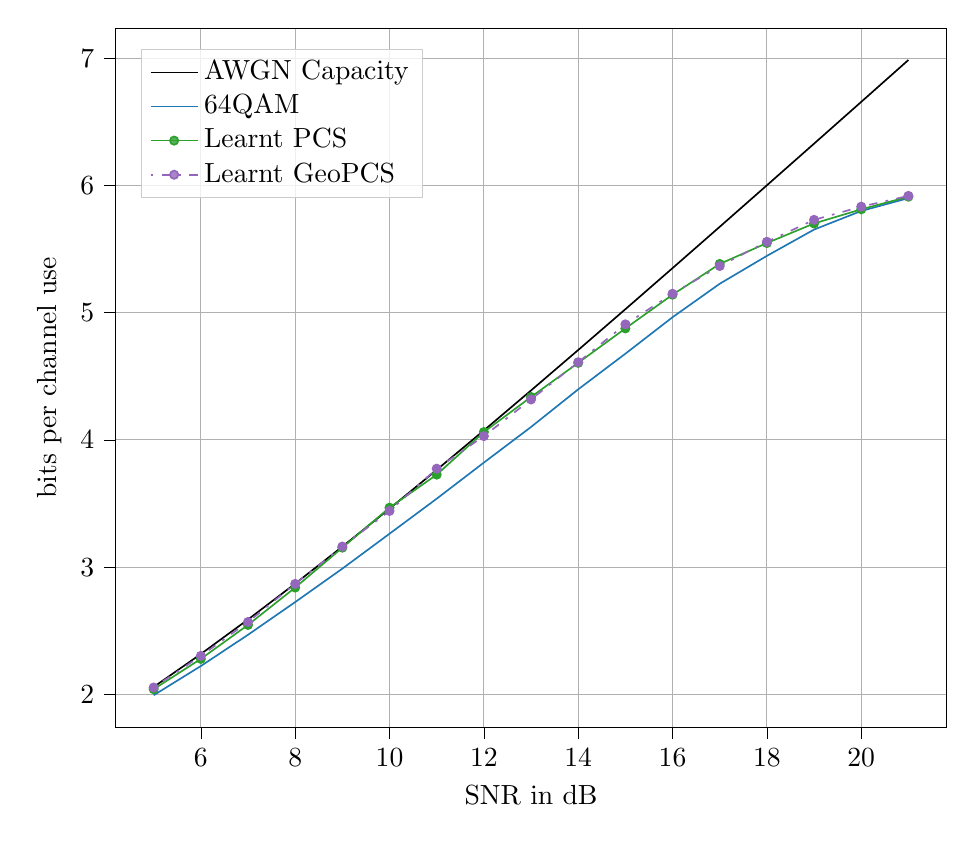
\begin{tikzpicture}

\definecolor{darkgray176}{RGB}{176,176,176}
\definecolor{forestgreen4416044}{RGB}{44,160,44}
\definecolor{lightgray204}{RGB}{204,204,204}
\definecolor{mediumpurple148103189}{RGB}{148,103,189}
\definecolor{steelblue31119180}{RGB}{31,119,180}

\begin{axis}[
width=1\columnwidth,
legend cell align={left},
legend style={
  fill opacity=0.8,
  draw opacity=1,
  text opacity=1,
  at={(0.03,0.97)},
  anchor=north west,
  draw=lightgray204
},
tick align=outside,
tick pos=left,
x grid style={darkgray176},
xlabel={SNR in dB},
xmajorgrids,
xmin=4.2, xmax=21.8,
xtick style={color=black},
y grid style={darkgray176},
ylabel={bits per channel use},
ymajorgrids,
ymin=1.74126489500718, ymax=7.23728243819158,
ytick style={color=black}
]
\addplot [semithick, black]
table {%
5 2.0573732086068
6 2.31645617962626
7 2.58781437356203
8 2.86978721917029
9 3.16080442391302
10 3.4594316186373
11 3.76439436704286
12 4.07458523490543
13 4.38905896736305
14 4.70702026272884
15 5.02780767335052
16 5.3508761542486
17 5.67577990180488
18 6.00215644400198
19 6.32971245944191
20 6.65821148275179
21 6.98746345895592
};
\addlegendentry{AWGN Capacity}
\addplot [semithick, steelblue31119180]
table {%
5 1.99252056510562
6 2.22188472335438
7 2.46783010150158
8 2.72497762849336
9 2.98797481594902
10 3.26241611912443
11 3.53780680098415
12 3.82177960231084
13 4.10180988838577
14 4.3977281031029
15 4.67794065159212
16 4.96490024705524
17 5.22792292071708
18 5.44727967105006
19 5.65395561651234
20 5.80023460021518
21 5.90134552221041
};
\addlegendentry{64QAM}
\addplot [semithick, forestgreen4416044, mark=*, mark size=1.5, mark options={solid}]
table {%
5 2.0399120192814
6 2.27815477000743
7 2.545269624195
8 2.83913156421006
9 3.15282104007778
10 3.46721977239767
11 3.72686335626646
12 4.06197533509096
13 4.33772578214366
14 4.60597916147994
15 4.87677306853477
16 5.14192078516177
17 5.38382229480225
18 5.54814724615274
19 5.70199948596159
20 5.81331697655905
21 5.9123535300237
};
\addlegendentry{Learnt PCS}
\addplot [semithick, mediumpurple148103189, dash pattern=on 1pt off 3pt on 3pt off 3pt, mark=*, mark size=1.5, mark options={solid}]
table {%
5 2.05332838587521
6 2.3021085136196
7 2.56858359234596
8 2.86818304557645
9 3.16180025427933
10 3.44141411960101
11 3.77398729053347
12 4.02976470441087
13 4.31813076683495
14 4.61100415057285
15 4.90888670099978
16 5.1493614425687
17 5.36734670081489
18 5.55776038840537
19 5.73043337762874
20 5.83422181173673
21 5.91892533107847
};
\addlegendentry{Learnt GeoPCS}
\end{axis}

\end{tikzpicture}

		\label{subfig:starkPerf}
	}
	\subfigure{
		\scalebox{0.8}{%% Creator: Matplotlib, PGF backend
%%
%% To include the figure in your LaTeX document, write
%%   \input{<filename>.pgf}
%%
%% Make sure the required packages are loaded in your preamble
%%   \usepackage{pgf}
%%
%% Also ensure that all the required font packages are loaded; for instance,
%% the lmodern package is sometimes necessary when using math font.
%%   \usepackage{lmodern}
%%
%% Figures using additional raster images can only be included by \input if
%% they are in the same directory as the main LaTeX file. For loading figures
%% from other directories you can use the `import` package
%%   \usepackage{import}
%%
%% and then include the figures with
%%   \import{<path to file>}{<filename>.pgf}
%%
%% Matplotlib used the following preamble
%%   \usepackage{fontspec}
%%   \setmainfont{DejaVuSerif.ttf}[Path=\detokenize{/home/ddeandres/Projects/internship_pcs/venv/lib/python3.10/site-packages/matplotlib/mpl-data/fonts/ttf/}]
%%   \setsansfont{DejaVuSans.ttf}[Path=\detokenize{/home/ddeandres/Projects/internship_pcs/venv/lib/python3.10/site-packages/matplotlib/mpl-data/fonts/ttf/}]
%%   \setmonofont{DejaVuSansMono.ttf}[Path=\detokenize{/home/ddeandres/Projects/internship_pcs/venv/lib/python3.10/site-packages/matplotlib/mpl-data/fonts/ttf/}]
%%
\begingroup%
\makeatletter%
\begin{pgfpicture}%
\pgfpathrectangle{\pgfpointorigin}{\pgfqpoint{4.000000in}{4.000000in}}%
\pgfusepath{use as bounding box, clip}%
\begin{pgfscope}%
\pgfsetbuttcap%
\pgfsetmiterjoin%
\pgfsetlinewidth{0.000000pt}%
\definecolor{currentstroke}{rgb}{1.000000,1.000000,1.000000}%
\pgfsetstrokecolor{currentstroke}%
\pgfsetstrokeopacity{0.000000}%
\pgfsetdash{}{0pt}%
\pgfpathmoveto{\pgfqpoint{0.000000in}{0.000000in}}%
\pgfpathlineto{\pgfqpoint{4.000000in}{0.000000in}}%
\pgfpathlineto{\pgfqpoint{4.000000in}{4.000000in}}%
\pgfpathlineto{\pgfqpoint{0.000000in}{4.000000in}}%
\pgfpathlineto{\pgfqpoint{0.000000in}{0.000000in}}%
\pgfpathclose%
\pgfusepath{}%
\end{pgfscope}%
\begin{pgfscope}%
\pgfsetbuttcap%
\pgfsetmiterjoin%
\definecolor{currentfill}{rgb}{1.000000,1.000000,1.000000}%
\pgfsetfillcolor{currentfill}%
\pgfsetlinewidth{0.000000pt}%
\definecolor{currentstroke}{rgb}{0.000000,0.000000,0.000000}%
\pgfsetstrokecolor{currentstroke}%
\pgfsetstrokeopacity{0.000000}%
\pgfsetdash{}{0pt}%
\pgfpathmoveto{\pgfqpoint{0.500000in}{0.500000in}}%
\pgfpathlineto{\pgfqpoint{3.600000in}{0.500000in}}%
\pgfpathlineto{\pgfqpoint{3.600000in}{3.520000in}}%
\pgfpathlineto{\pgfqpoint{0.500000in}{3.520000in}}%
\pgfpathlineto{\pgfqpoint{0.500000in}{0.500000in}}%
\pgfpathclose%
\pgfusepath{fill}%
\end{pgfscope}%
}
%		% This file was created with tikzplotlib v0.10.1.
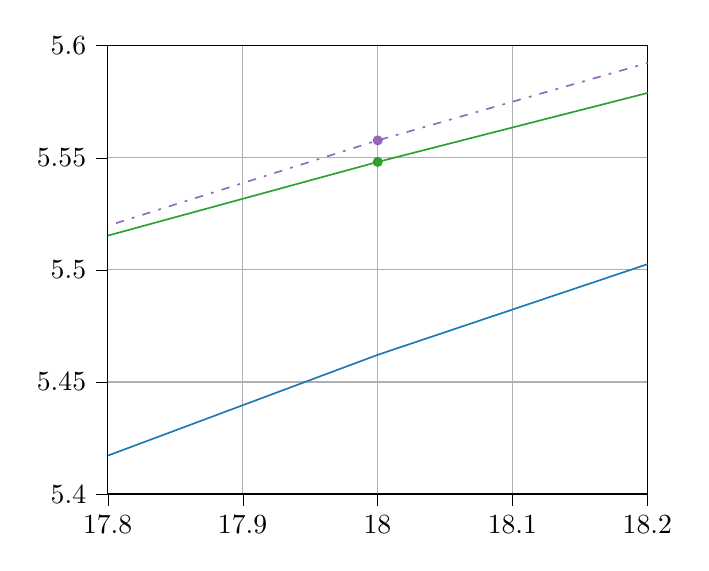
\begin{tikzpicture}

\definecolor{darkgray176}{RGB}{176,176,176}
\definecolor{forestgreen4416044}{RGB}{44,160,44}
\definecolor{mediumpurple148103189}{RGB}{148,103,189}
\definecolor{steelblue31119180}{RGB}{31,119,180}

\begin{axis}[
%width=0.3\columnwidth,
%height=5cm,
tick align=outside,
tick pos=left,
x grid style={darkgray176},
xmajorgrids,
xmin=17.8, xmax=18.2,
xtick style={color=black},
y grid style={darkgray176},
ymajorgrids,
ymin=5.4, ymax=5.6,
ytick style={color=black}
]
\addplot [semithick, black]
table {%
5 2.0573732086068
6 2.31645617962626
7 2.58781437356203
8 2.86978721917029
9 3.16080442391302
10 3.4594316186373
11 3.76439436704286
12 4.07458523490543
13 4.38905896736305
14 4.70702026272884
15 5.02780767335052
16 5.3508761542486
17 5.67577990180488
18 6.00215644400198
19 6.32971245944191
20 6.65821148275179
21 6.98746345895592
};
\addplot [semithick, steelblue31119180]
table {%
5 1.99108387424284
6 2.24402647460228
7 2.50971018391181
8 2.7168062393637
9 3.01798305343714
10 3.29181687976594
11 3.53995062094712
12 3.82640037464754
13 4.14023692975961
14 4.39354709644104
15 4.70346129879599
16 4.98856046498287
17 5.23734812190524
18 5.46209867864363
19 5.6643156062385
20 5.81125953714345
21 5.90157509420288
};
\addplot [semithick, forestgreen4416044, mark=*, mark size=1.5, mark options={solid}]
table {%
5 2.0399120192814
6 2.27815477000743
7 2.545269624195
8 2.83913156421006
9 3.15282104007778
10 3.46721977239767
11 3.72686335626646
12 4.06197533509096
13 4.33772578214366
14 4.60597916147994
15 4.87677306853477
16 5.14192078516177
17 5.38382229480225
18 5.54814724615274
19 5.70199948596159
20 5.81331697655905
21 5.9123535300237
};
\addplot [semithick, mediumpurple148103189, dash pattern=on 1pt off 3pt on 3pt off 3pt, mark=*, mark size=1.5, mark options={solid}]
table {%
5 2.05332838587521
6 2.3021085136196
7 2.56858359234596
8 2.86818304557645
9 3.16180025427933
10 3.44141411960101
11 3.77398729053347
12 4.02976470441087
13 4.31813076683495
14 4.61100415057285
15 4.90888670099978
16 5.1493614425687
17 5.36734670081489
18 5.55776038840537
19 5.73043337762874
20 5.83422181173673
21 5.91892533107847
};
\end{axis}

\end{tikzpicture}

		\label{subfig:starkPerfZoom}
	}
    \caption{\subref{subfig:starkPerf} Mutual information learned by the PCS and GeoPCS for constellation size M=64 on the AWGN channel}.
    \label{fig:starkPerf}
\end{figure}


\section{Second implementation}
In this section we break-down the autoencoder system presented by \citet{Aref}. This novel approach calls to remove the risk of numerical instabilities present in \cite{Stark}. Such instabilities are introduced by the Gumbel-Softmax trick, required to make the sampler differentiable, and the sensitive extra hyper-parameters. The outstanding feature of this autoencoder is the hability to sample from the constellation probabilities without any approximation.

\subsection{Optimization of trainable parameters}
\label{sec:parameters}
As we have seen in Chapter \ref{chap:preliminaries}, the goal of probabilistic constellation shaping is to maximize the mutual information
\begin{align}
	 \max_{D, P_M, C_M} \mathbb{I} \left(X , Y ; D, P_M, C_M \right) = \mathbb{H}(X) - \mathbb{X}(P_{X|Y} \Vert Q_{X|Y} ; D, P_M, C_M)
\end{align}

where the entropy is maximized when the symbols probabilities follow a \cgls{mb} distribution; and the cross-equivocation is minimum when $Q_{X|Y} = P_{X|Y}$.

Typically, the gradient descent (or ascent, as we intent to maximize) allows us to solve the optimization problem by adjusting the trainable parameters as:
\begin{align}
	\theta_{new} = \theta_{old} + \epsilon \pdv{\theta_{old}} \mathbb{I} \left(X , Y ; \theta_{old} \right)
\end{align}
for all trainable parameters $\theta \in P_M, C_M, D$. And the \cgls{mi} can be numerically approximated by
\begin{align}
	\mathbb{I} \left(X , Y\right) \approx \mathbb{I} \left(X , Y\right)_{\text{num}} &= \dfrac{1}{B} \sum \limits_{i = 1}^{B} - \log_2(P(x_i)) + \log_2(Q_{X|Y}(x_i|y_i))\\
	&= \dfrac{1}{B} \sum \limits_{i = 1}^{B} L(x_i, y_i).
\end{align}

Next, the following approximation usually allows to adjust the trainable parameters:
\begin{align}
	\pdv{\theta} \mathbb{I} \left(X , Y ; \theta \right) \approx \pdv{\theta} \mathbb{I} \left(X , Y\right)_{\text{num}} = \dfrac{1}{B} \sum \limits_{i = 1}^{B} L(x_i, y_i).
\end{align}

However, Aref claims that although this is true for the constellation locations $(\theta \in C_M)$ and the demapper parameters $(\theta \in D)$, it does not hold for the constellation probabilities $\{p_1, p_2, \dots, p_M\} = P_M$
\begin{align}
\label{eqn:mi_pdv_p}
	\pdv{p_j} \mathbb{I} \left(X , Y ; P_M \right) \not\approx \dfrac{1}{B} \sum \limits_{i = 1}^{B} \pdv{p_j} L(x_i, y_i)
\end{align}

as $\{p_1, p_2, \dots, p_M\}$ changes the statistics of the training set.

For this reason, (\ref{eqn:mi_pdv_p}) must be computed differently. On the one hand, to compute the derivative of the cross-equivocation, the following expansions are useful
\begin{align}
	\mathbb{X}\left(P_{X|Y} \Vert Q_{X|Y} \vert Y=b \right) = \sum \limits_{a \in Supp(P_{X|Y}(\cdot|b))} P_{X|Y}(a|b) \log_2(Q_{X|Y}(a|b))
\end{align}

\begin{align}
	\mathbb{X}\left(P_{X|Y} \Vert Q_{X|Y}\right) = \sum \limits_{b \in Supp(P_Y)} P_Y(b) \mathbb{X}\left( P_{X|Y} \Vert Q_{X|Y} \vert Y=b \right) 
\end{align}

as combined together and applying Bayes' theorem they yield

\begin{align}
\label{eqn:CE_expanded}
	\mathbb{X}\left(P_{X|Y} \Vert Q_{X|Y}\right) = \sum \limits_{(a,b) \in Supp(P_{XY})} P_X(a) P_{Y|X}(b|a) \log_2(Q_{X|Y}(a|b)). 
\end{align}

And so, the derivative results
\begin{align}
	\pdv{p_j} \mathbb{X}\left(P_{X|Y} \Vert Q_{X|Y}\right) &= \sum \limits_{b \text{ if } x=j} P_{Y|X}(b|j) \log_2 Q_{X|Y}(j|b) \\
	& + \sum \limits_{(a,b) \in Supp(P_{XY})} P_{XY}(a, b) \pdv{p_j} \log_2 Q_{X|Y}(a|b)
\end{align}
which can be rewritten using the expectation operator as
\begin{align}
	\pdv{p_j} \mathbb{X}\left(P_{X|Y} \Vert Q_{X|Y}\right) &= \mathbb{E}_{Y|X}[ \log_2 Q_{X|Y}(j|b)| X=j] \\
	& + \mathbb{E}_{XY}[ \pdv{p_j} \log_2 Q_{X|Y}(a|b)].
\end{align}
The terms can now be numerically computed as
\begin{align}
\label{eqn:CE_term_1}
	\mathbb{E}_{Y|X}[ \log_2 Q_{X|Y}(j|b)| X=j] \approx \dfrac{1}{Bp_j}\sum \limits_{b \text{ if } x=j} \log_2 Q_{X|Y}(j|b)
\end{align}
\begin{align}
\label{eqn:CE_term_2}
	\mathbb{E}_{XY}[ \pdv{p_j} \log_2 Q_{X|Y}(a|b)] \approx \dfrac{1}{B} \sum \limits_{(a,b) \in Supp(P_{XY})} \log_2 Q_{X|Y}(a|b).
\end{align}
On the other hand, the derivative of the entropy w.r.t. $p_j$ is
\begin{align}
\label{eqn:H_term_1}
	\pdv{p_j} \mathbb{H}(X) = \pdv{p_j} \sum \limits_{i = 1}^{B} - p_i \log_2(p_i) = - \log_2 (p_j) - log_2 (e).
\end{align}

Now, combining (\ref{eqn:CE_term_1}), (\ref{eqn:CE_term_2}), and (\ref{eqn:H_term_1}) the derivative of the mutual information w.r.t. $p_j$, (\ref{eqn:mi_pdv_p}), can be computed as
\begin{align}
	\pdv{p_j} \mathbb{I} \left(X , Y ; P_M \right) \approx - \log_2 (p_j) - \log_2 (e) + \dfrac{1}{Bp_j}\sum \limits_{b \text{ if } x=j} \log_2 Q_{X|Y}(j|b) + \dfrac{1}{B} \sum \limits_{(a,b)} \log_2 Q_{X|Y}(a|b)
\end{align}

Aref now indicates that the following terms can be computed via backpropagation
\begin{align}
	- \log_2 (p_j) + \dfrac{1}{Bp_j}\sum \limits_{b \text{ if } x=j} \log_2 Q_{X|Y}(j|b) = \dfrac{1}{B} \sum \limits_{i = 1}^{B} \pdv{p_j} L(x_i, y_i)
\end{align}
while the remaining ones must be explicitely computed and added to the gradient after backpropagating. We call this step \textit{gradient correction} and it is due to the change of statistics in the sampled batch.

\subsection{Autoencoder Architecture}
\begin{figure}[H]
	\centering
	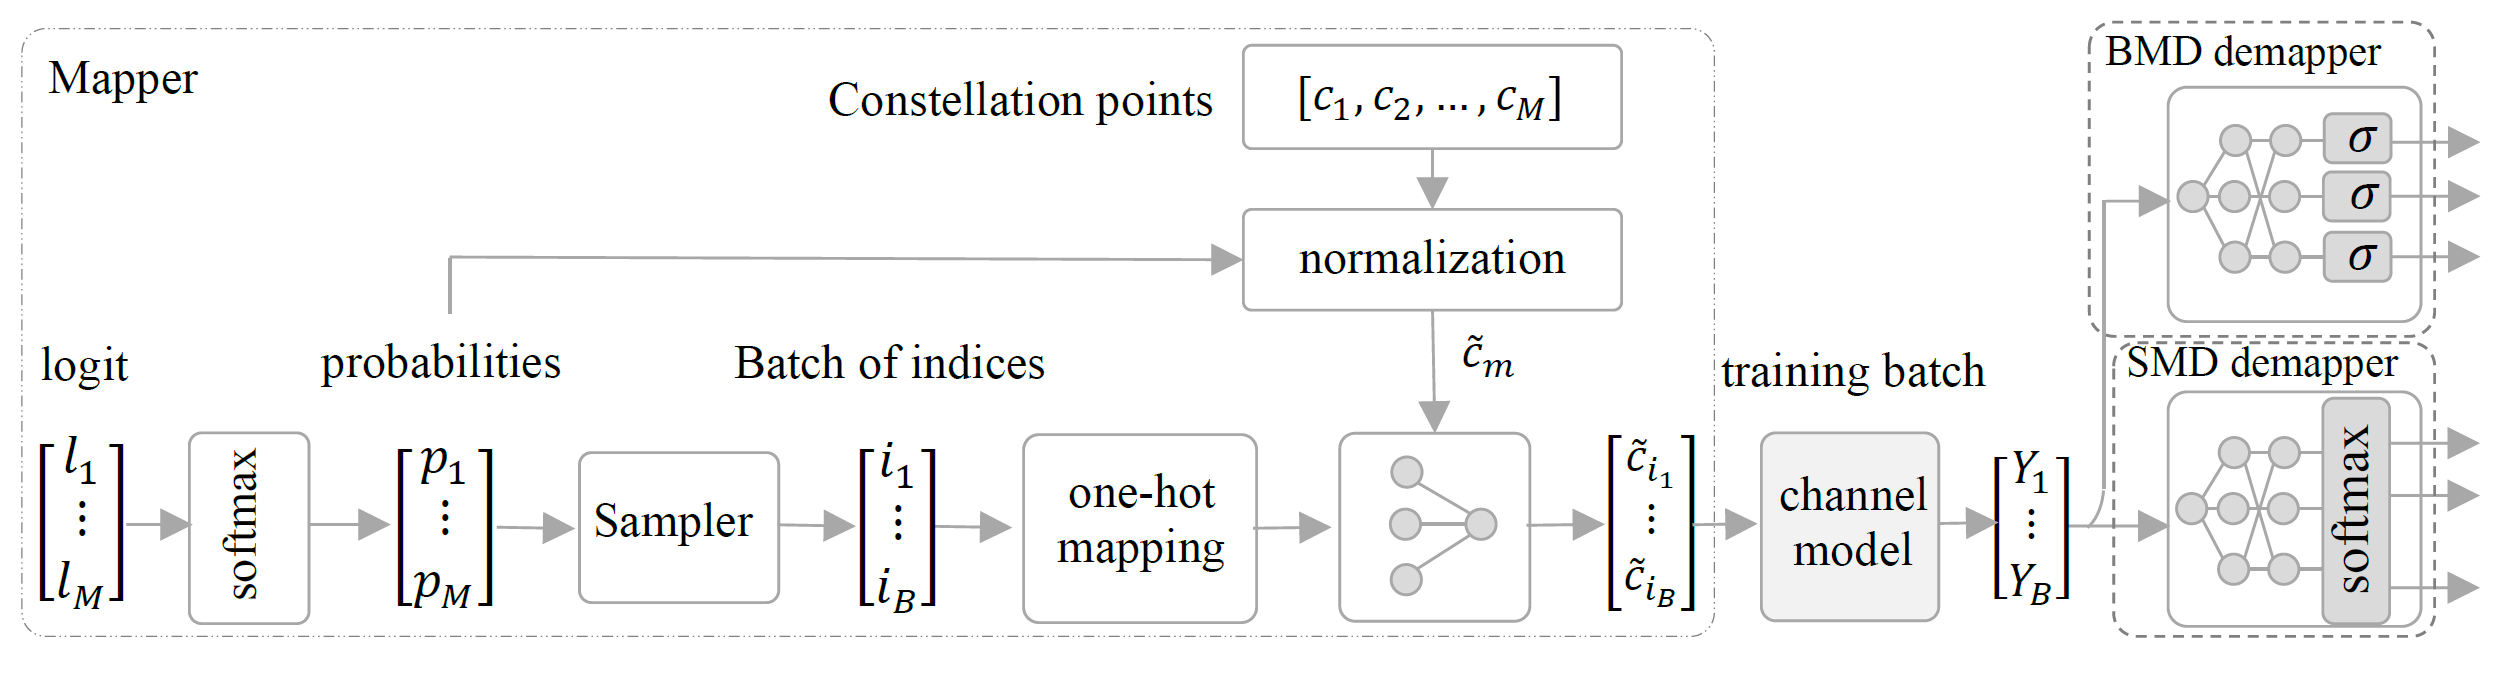
\includegraphics[width=\textwidth]{figs/aref_diagram.png}
	\caption{Proposed Autoencoder Architecture from \cite{Aref}}
	\label{fig:arefAe}
\end{figure}

\citeauthor{Aref}'s autoencoder is made up from two major blocks: mapper and demapper. Fig \ref{fig:arefAe} shows the complete architecture of the end-to-end system, where the trainable parameters are  $P_M, C_M, \text{ and } D$. Furthermore, the mapper breaks down into the sampling and the modulation mechanism. In order to sample, a single linear layer followed by a softmax layer trains the $p_i \in P_M$. Next, to produce a training symbols batch of size B, each index $i$ is drawn about $Bp_i$ times, for $i = 1, \dots, M$. After, the indeces are randomly permuted. Note that this sampling mechanism is not differentiable and consequently, the derivatives of the loss function w.r.t to the $p_i$ will not be accurate. However, using the \textit{gradient correction} factor described in Section \ref{sec:parameters}, the gradient is adjusted during the backpropagation step. Similar to the previously presented architecture, the modulation mechanism is made of a single linear layer of M units and trainable parameters $c_i \in C_M$. It also includes a normalization layer to ensure that the power contstraints are met. Finally, the Demapper is also made of a single linear layer followed by a softmax layer. The demapper's trainable parameter, $D$ correspond to the \textit{a posteriori} probability distribution $p(x|y)$ depending on the channel model.

\subsection{Autoencoder Performance}
Training was performed with the Adam optimizer and the hyper-parameters of the training are: learning-rate=0.1, batch-size=10000, and number of epochs=4000.
The resulting M-\cgls{ask} constellations for both only probabilistic and joint probabilistic and geometric shaping are presented in Figure \ref{fig:arefMASK}. Moreover the respective achieved \cgls{mi} for the corresponding M-\cgls{qam} scheme, i.e., 64-\cgls{qam}, are available in Figure \ref{fig:arefPerf} for SNR values ranging from 5dB to 22dB.

\begin{figure}
	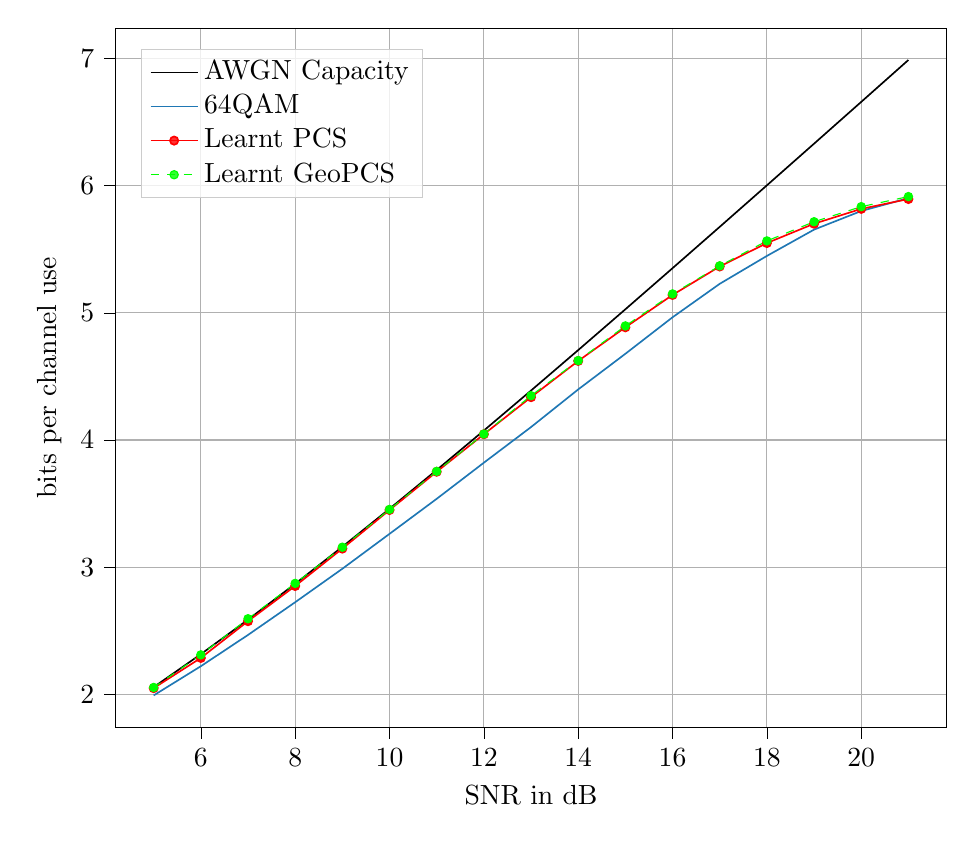
\begin{tikzpicture}

\definecolor{darkgray176}{RGB}{176,176,176}
\definecolor{lightgray204}{RGB}{204,204,204}
\definecolor{steelblue31119180}{RGB}{31,119,180}

\begin{axis}[
width=\columnwidth,
legend cell align={left},
legend style={
  fill opacity=0.8,
  draw opacity=1,
  text opacity=1,
  at={(0.03,0.97)},
  anchor=north west,
  draw=lightgray204
},
tick align=outside,
tick pos=left,
x grid style={darkgray176},
xlabel={SNR in dB},
xmajorgrids,
xmin=4.2, xmax=21.8,
xtick style={color=black},
y grid style={darkgray176},
ylabel={bits per channel use},
ymajorgrids,
ymin=1.7427734204131, ymax=7.23721060364844,
ytick style={color=black}
]
\addplot [semithick, black]
table {%
5 2.0573732086068
6 2.31645617962626
7 2.58781437356203
8 2.86978721917029
9 3.16080442391302
10 3.4594316186373
11 3.76439436704286
12 4.07458523490543
13 4.38905896736305
14 4.70702026272884
15 5.02780767335052
16 5.3508761542486
17 5.67577990180488
18 6.00215644400198
19 6.32971245944191
20 6.65821148275179
21 6.98746345895592
};
\addlegendentry{AWGN Capacity}
\addplot [semithick, steelblue31119180]
table {%
5 1.99252056510562
6 2.22188472335438
7 2.46783010150158
8 2.72497762849336
9 2.98797481594902
10 3.26241611912443
11 3.53780680098415
12 3.82177960231084
13 4.10180988838577
14 4.3977281031029
15 4.67794065159212
16 4.96490024705524
17 5.22792292071708
18 5.44727967105006
19 5.65395561651234
20 5.80023460021518
21 5.90134552221041
};
\addlegendentry{64QAM}
\addplot [semithick, red, mark=*, mark size=1.5, mark options={solid}]
table {%
5 2.04953616842369
6 2.28690524728333
7 2.57595580065785
8 2.8524662390447
9 3.14655158452323
10 3.44979861779587
11 3.7504920526685
12 4.04539311186007
13 4.33694188522102
14 4.62174584298044
15 4.8859686369111
16 5.14053322913461
17 5.36437105698967
18 5.54836875980705
19 5.70036840250081
20 5.81702285871985
21 5.89450310672535
};
\addlegendentry{Learnt PCS}
\addplot [dashed, green, mark=*, mark size=1.5, mark options={solid}]
table {%
5 2.054870726288148
6 2.3113123371631734
7 2.5950424352506007
8 2.872956939999102
9 3.157409537202804
10 3.4543671649333914
11 3.7535450886866175
12 4.0472924882562
13 4.348614691700384
14 4.624498253324846
15 4.896956264509424
16 5.148696901605764
17 5.369250548759946
18 5.565256424225875
19 5.715805221276954
20 5.8343876030121615
21 5.913611755097416
};
\addlegendentry{Learnt GeoPCS}
\end{axis}

\end{tikzpicture}
	\caption{Mutual information learned by the probabilistic constellation shpaing on the AWGN channel.}
	\label{fig:arefPerf}
\end{figure}

